\documentclass[phdthesis,12pt,final]{wuthesis}

\usepackage{lmodern}

\usepackage{setspace}
\setstretch{2}

% Remove or comment out the following lines as they're now in wuthesis.tex
% \documentclass[phdthesis,12pt,final]{wuthesis}



\usepackage{ifluatex}
\ifluatex
  \usepackage{fontspec} % international characters
  \usepackage{polyglossia}
  \setmainlanguage[variant=american]{english}
\else % use for pdflatex
  \usepackage[utf8]{inputenc}
  \usepackage[T1]{fontenc}
  \usepackage[american]{babel}
\fi

\usepackage{booktabs}
\usepackage{fancyhdr} % for pagination
\usepackage{microtype} % typographical perfection
\usepackage{csquotes}
\usepackage[vskip=0pt,begintext=\textooquote,endtext=\textcoquote]{quoting}
\SetBlockEnvironment{quoting}

\usepackage[
  backend=biber,
  isbn=false,
  url=false,
  sortcites,
  maxbibnames=8
]{biblatex}

% customzing fonts
\usepackage{titlesec}
\usepackage{tocloft}
\usepackage{anyfontsize}

% Define a consistent font size for title and chapters
\newcommand{\maintitlesize}{\fontsize{16}{20}\selectfont}

% Center and format chapter headings
\titleformat{\chapter}[display]
{\normalfont\maintitlesize\bfseries\centering}
{\chaptertitlename\ \thechapter}{20pt}{\maintitlesize}
\titlespacing*{\chapter}{0pt}{-50pt}{40pt}

% change section headings font size
\titleformat{\section}
{\normalfont\large\bfseries}{\thesection}{1em}{}

% Format List of Tables
\renewcommand{\cfttoctitlefont}{\hfill\maintitlesize\bfseries}
\renewcommand{\cftaftertoctitle}{\hfill}
\renewcommand{\cftlottitlefont}{\hfill\maintitlesize\bfseries}
\renewcommand{\cftafterlottitle}{\hfill}

% Format List of Figures
\renewcommand{\cftloftitlefont}{\hfill\maintitlesize\bfseries}
\renewcommand{\cftafterloftitle}{\hfill}

% Adjust spacing for List of Tables and List of Figures
\setlength{\cftbeforelottitleskip}{-50pt}
\setlength{\cftbeforeloftitleskip}{-50pt}
\setlength{\cftaftertoctitleskip}{40pt}
\setlength{\cftafterlottitleskip}{40pt}
\setlength{\cftafterloftitleskip}{40pt}

% Single-space within entries, double-space between entries
\renewcommand{\cftbeforetabskip}{2em}
\renewcommand{\cftbeforefigskip}{2em}

% general packages
\usepackage{amsmath}
\usepackage{amsfonts}
\usepackage[section]{placeins} % stop floats at sections
\usepackage[inline, shortlabels]{enumitem}
\usepackage{threeparttable}
\usepackage{array}
\usepackage{siunitx}
\usepackage{makecell}
\newcommand{\stretchtable}[1][1.4]{\renewcommand{\arraystretch}{#1}}
\usepackage{mdframed}

% ensure vitaauctoris always starts on a new page
\usepackage{etoolbox}
\pretocmd{\chapter}{\clearpage}{}{}

% use links in document. load last.
\usepackage[hidelinks,linktoc=all]{hyperref}
\usepackage[noabbrev]{cleveref}
\newcommand{\crefrangeconjunction}{--}
\usepackage{caption}

\providecommand{\tightlist}{%
  \setlength{\itemsep}{0pt}\setlength{\parskip}{0pt}}

% for bib
\addbibresource{book.bib}

% style something
\usepackage{fancyvrb}
\usepackage{xcolor}

% Define Shaded and Highlighting environments
\newenvironment{Shaded}{}{}
\newenvironment{Highlighting}{}{}

% Define syntax highlighting commands
\newcommand{\pandocbounded}[1]{#1}

\newcommand{\AttributeTok}[1]{\textcolor[rgb]{0.77,0.63,0.00}{\textbf{#1}}}
\newcommand{\FunctionTok}[1]{\textcolor[rgb]{0.00,0.00,0.75}{#1}}
\newcommand{\NormalTok}[1]{#1}
\newcommand{\ConstantTok}[1]{\textcolor[rgb]{0.53,0.00,0.00}{#1}}
\newcommand{\StringTok}[1]{\textcolor[rgb]{0.31,0.60,0.02}{#1}}
\newcommand{\KeywordTok}[1]{\textcolor[rgb]{0.13,0.29,0.53}{\textbf{#1}}}
\newcommand{\DataTypeTok}[1]{\textcolor[rgb]{0.13,0.29,0.53}{#1}}
\newcommand{\CommentTok}[1]{\textcolor[rgb]{0.56,0.35,0.01}{\textit{#1}}}
\newcommand{\OtherTok}[1]{\textcolor[rgb]{0.56,0.35,0.01}{#1}}
\newcommand{\OperatorTok}[1]{\textcolor[rgb]{0.00,0.00,0.00}{#1}}
\newcommand{\ErrorTok}[1]{\textcolor[rgb]{0.64,0.00,0.00}{\textbf{#1}}}
\newcommand{\WarningTok}[1]{\textcolor[rgb]{0.56,0.35,0.01}{\textbf{\textit{#1}}}}

% Additional syntax highlighting commands for R code
\newcommand{\DecValTok}[1]{\textcolor[rgb]{0.00,0.00,0.81}{#1}}
\newcommand{\BaseNTok}[1]{\textcolor[rgb]{0.00,0.00,0.81}{#1}}
\newcommand{\FloatTok}[1]{\textcolor[rgb]{0.00,0.00,0.81}{#1}}
\newcommand{\CharTok}[1]{\textcolor[rgb]{0.31,0.60,0.02}{#1}}
\newcommand{\SpecialCharTok}[1]{\textcolor[rgb]{0.00,0.00,0.00}{#1}}
\newcommand{\SpecialStringTok}[1]{\textcolor[rgb]{0.31,0.60,0.02}{#1}}
\newcommand{\VerbatimStringTok}[1]{\textcolor[rgb]{0.31,0.60,0.02}{#1}}
\newcommand{\ImportTok}[1]{#1}
\newcommand{\ControlFlowTok}[1]{\textcolor[rgb]{0.00,0.44,0.13}{\textbf{#1}}}
\newcommand{\BuiltInTok}[1]{#1}
\newcommand{\ExtensionTok}[1]{#1}
\newcommand{\PreprocessorTok}[1]{\textcolor[rgb]{0.56,0.35,0.01}{\textit{#1}}}
\newcommand{\DocumentationTok}[1]{\textcolor[rgb]{0.56,0.35,0.01}{\textbf{\textit{#1}}}}
\newcommand{\AnnotationTok}[1]{\textcolor[rgb]{0.56,0.35,0.01}{\textbf{\textit{#1}}}}
\newcommand{\CommentVarTok}[1]{\textcolor[rgb]{0.56,0.35,0.01}{\textbf{\textit{#1}}}}
\newcommand{\VariableTok}[1]{\textcolor[rgb]{0.00,0.00,0.00}{#1}}
\newcommand{\InformationTok}[1]{\textcolor[rgb]{0.56,0.35,0.01}{\textbf{\textit{#1}}}}

%%%%%%%%%%%%%%%%%%%%%%%%%%%%%%%%%%%%%%%%%%%%%%%%%%%%%%%%%%%%%%%%%%%%%%%%%%%%%
%%
%% These commands customize the `wuthesis' package for me
%%
%%%%%%%%%%%%%%%%%%%%%%%%%%%%%%%%%%%%%%%%%%%%%%%%%%%%%%%%%%%%%%%%%%%%%%%%%%%%%

%% Enter your official name
\renewcommand{\thesisauthor}{Montaque Reynolds}
\renewcommand{\thesisauthorlastname}{Reynolds}

%% Enter your previous degrees
%% If you have no previous degrees remember to remove the comma too.
\renewcommand{\thesisauthorpreviousdegrees}{, M.A.}

%% Enter department name
\renewcommand{\thesisdepartment}{Department of Philosophy}
\renewcommand{\thesisfield}{Philosophy}

%% Enter date of graduation
\renewcommand{\thesismonth}{August}
\renewcommand{\thesisyear}{2024}

%% Enter title of thesis
\renewcommand{\thesistitle}{EMOTIONAL DATA AND THE MORAL EXPRESSIONS OF SENTIMENT IN FICTION}

%% Enter the copyright holder ( DEFAULT is \thesisauthor )
%\renewcommand{\thesiscopyrightholder}{\thesisauthor}

%% Enter supervisor name
\renewcommand{\thesissupervisor}{Professor Dan Haybron, Chair\\
Scott Ragland, Co-Chair}
%%
% list in alphabetical order
%%
\renewcommand{\thesiscommittee}{Dan Haybron, Chair\\
Scott Ragland, Co-Chair \\
Scott Gelfand \\
Helen De Cruz}

\renewcommand{\thesisdedication}{Dedicated to my parents.}

\hypersetup{
  pdftitle={\thesistitle},
  pdfauthor={\thesisauthor},
  pdfpagemode=UseOutlines,
  bookmarksnumbered=true,
  bookmarksopen=true,
  bookmarksopenlevel=1
}


% definitions for citeproc citations
\NewDocumentCommand\citeproctext{}{}
\NewDocumentCommand\citeproc{mm}{%
\begingroup\def\citeproctext{#2}\cite{#1}\endgroup}
\makeatletter
% allow citations to break across lines
\let\@cite@ofmt\@firstofone
% avoid brackets around text for \cite:
\def\@biblabel#1{}
\def\@cite#1#2{{#1\if@tempswa , #2\fi}}
\makeatother
\newlength{\cslhangindent}
\setlength{\cslhangindent}{1.5em}
\newlength{\csllabelwidth}
\setlength{\csllabelwidth}{3em}
\newenvironment{CSLReferences}[2] % #1 hanging-indent, #2 entry-spacing
{\begin{list}{}{%
	\setlength{\itemindent}{0pt}
	\setlength{\leftmargin}{0pt}
	\setlength{\parsep}{0pt}
	% turn on hanging indent if param 1 is 1
	\ifodd #1
	\setlength{\leftmargin}{\cslhangindent}
	\setlength{\itemindent}{-1\cslhangindent}
	\fi
	% set entry spacing
	\setlength{\itemsep}{#2\baselineskip}}}
{\end{list}}
\usepackage{calc}
\newcommand{\CSLBlock}[1]{\hfill\break\parbox[t]{\linewidth}{\strut\ignorespaces#1\strut}}
\newcommand{\CSLLeftMargin}[1]{\parbox[t]{\csllabelwidth}{\strut#1\strut}}
\newcommand{\CSLRightInline}[1]{\parbox[t]{\linewidth - \csllabelwidth}{\strut#1\strut}}
\newcommand{\CSLIndent}[1]{\hspace{\cslhangindent}#1}

\usepackage{amsthm}
\newtheorem{theorem}{Theorem}[chapter]
\newtheorem{lemma}{Lemma}[chapter]
\newtheorem{corollary}{Corollary}[chapter]
\newtheorem{proposition}{Proposition}[chapter]
\newtheorem{conjecture}{Conjecture}[chapter]
\theoremstyle{definition}
\newtheorem{definition}{Definition}[chapter]
\theoremstyle{definition}
\newtheorem{example}{Example}[chapter]
\theoremstyle{definition}
\newtheorem{exercise}{Exercise}[chapter]
\theoremstyle{definition}
\newtheorem{hypothesis}{Hypothesis}[chapter]
\theoremstyle{remark}
\newtheorem*{remark}{Remark}
\newtheorem*{solution}{Solution}
\begin{document}
% Title Page
\begin{titlepage}
\begin{center}
\vspace*{0.5in} % Adjust this value to move the title up or down

{\large\MakeUppercase{Emotional Data and The Moral Expressions of Sentiment in Fiction}\par}

\vspace{1.7in} % Adjust this space between title and author name

{\large Montaque Reynolds, \thesisauthorpreviousdegrees\par}

\vspace{3in} % Adjust this space as needed

A Dissertation Presented to the Graduate Faculty of\\
Saint Louis University in Partial Fulfillment\\
of the Requirements for the Degree of\\
Doctor of Philosophy

\vfill % This will push the year to the bottom of the page

2024

\end{center}
\end{titlepage}

\pagenumbering{roman}
\setcounter{page}{2}

% Copyright Page
\cleardoublepage
\thispagestyle{empty}
\begin{thesiscopyrightpage}
    \vspace*{\fill}
    \begin{center}
    \textcopyright\ Copyright by\\
    \thesisauthor\\
    ALL RIGHTS RESERVED\\
    \thesisyear
    \end{center}
    \vspace*{-10cm} % Adjust this value to fine-tune the vertical position
\end{thesiscopyrightpage}

% Committee Page
\cleardoublepage
\thispagestyle{empty}

\vspace*{\fill}

\noindent\thesiscommittee

\vspace*{10cm} % Adjust this value to fine-tune the vertical position


% Dedication Page (if applicable)

% Acknowledgement Page (if applicable)

% Table of Contents
\cleardoublepage
\begin{singlespace}
\setcounter{page}{2}
\renewcommand*\contentsname{Table of Contents}
\tableofcontents
\end{singlespace}

% List of Tables (if applicable)

% List of Figures (if applicable)

% Abstract

\cleardoublepage
\pagenumbering{arabic}
\setcounter{page}{1}

\chapter{Introduction}\label{introduction}

My dissertation addresses two central questions for social epistemologists: the value of moral testimony and how to appropriately respond to morally laden situations in fiction. According to some, reliance on moral testimony is untenable. Epistemologists Alison\footnote{\textbf{hill09?}; \textbf{hill13?}; Alison Hills, {``Understanding {Why},''} \emph{Noûs} 50, no. 4 (2016): 661--88, \url{https://www.jstor.org/stable/26631424}.} and Sarah\footnote{Sarah McGrath, {``The {Puzzle} of {Pure Moral Deference},''} \emph{Philosophical Perspectives} 23 (2009): 321--44, \url{https://www.jstor.org/stable/40658407}; Sarah McGrath and Journal of Philosophy, Inc., {``Skepticism about {Moral Expertise} as a {Puzzle} for {Moral Realism}:''} \emph{Journal of Philosophy} 108, no. 3 (2011): 111--37, \url{https://doi.org/10.5840/jphil201110837}.} have expressed worries that moral testimony, while potentially valuable, should not be acted on. Moral actions that are based on moral testimony would have no moral worth. However, some of the more plausible explanations share an important feature with the second central question. We often expect active agency in the context of moral behavior. It is not enough that we act rightly, but our actions ought to reflect our understanding regarding the correct action. Moral reflection, unlike non-moral reflection, however, requires a richer form of understanding involving both cognitive and non-cognitive faculties. The right emotion ought to accompany our moral action. Like (1), (2) also concerns emotions. We have emotions toward fictions, however, these do not always mirror those we have in the real world. In some situations, an emotional response to fiction is apt though inapt outside of such contexts, e.g., slap-stick comedy. The right emotion need not accompany the audience of art. Jonathan\footnote{\textbf{gilm21?}} argues that our emotions towards a given fiction is often justified just in case the emotion was the one intended by the author. The second problem then concerns the aptness of an expressed emotion. In chapter 2, I examine the relationship between fiction and the more robust form of moral understanding important for attributions of moral worth. I contrast standard epistemological cases with moral epistemological ones. Chapter 3 explores philosophical accounts of narrative. Following notable optimists in the literature on moral testimony, such as Eleanor Stump and Martha Nussbaum, I argue that narrative is a potential avenue for achieving affective moral understanding. I define affective moral understanding as feeling the right way at the right time in response to the right object. The philosophy of psychology literature often makes reference to the importance of identity for personal agency. It also addresses these concerns in moral epistemology regarding the importance of moral narratives for the construction of this identity. In chapter 4, I look at psychological accounts of narrative. I focus on a class of such accounts that draw a connection between narrative understanding and human flourishing. Following the psychology literature, I argue that human beings are social creatures, and as such, a prime component in human flourishing are our relationships with others. Therefore, narratives which contribute to our understanding of the importance of these relationships in our lives can be tools we use to ensure the well-being of those we love. Finally, in chapter 5, I consider whether literary narratives central to human flourishing are necessarily classical works of literature. The question about apt emotional expression and art is often articulated as a form of moral enhancement. Art is said to have the ability to make us better persons. For instance, Elizabeth Glaskill's ``Mary Barton'' is often credited with motivating the expanded public health care and other social goods that the United Kingdom provides. However, rarely is popular music discussed. Yet, it is likely that a greater proportion of a given population consume popular music rather then classical literature. I argue this raises a problem: if only classical works are central to human flourishing, then only classical works can potentially undermine human flourishing. So I expand my investigation to consider a class of non-classical works, namely popular narratives. Analyzing these narratives, I develop a model of non-classical literary works that satisfy both philosophical and psychological accounts of the close connection between narrative and human flourishing.

\section{The Ethics of Care and Caring Audiences}\label{the-ethics-of-care-and-caring-audiences}

In her 1982 book \emph{In a Different Voice}, Carol\footnote{\textbf{gill82?}} coins the term \emph{Ethic of Care}. Gilligan argues women treat moral issues in terms of emotional responses. When a care-giver wants to teach the harms of bullying, they will often encourage a child to imagine being bullied. Moral philosophers since, recognize the importance of empathy in both public and private life. Highlighting the centrality of emotional expression in moral matters, we revitalize the works of seventeenth century sentimentalists, Hume, Hutcheson, Smith, etc. The resurgence focuses our attention to classical moral views grounded in empathy. In book VIII of the Nicomachean Ethics, Aristotle defines his ideal social constitution. He first ranks three types of friendships, the best of which he calls \emph{friends of virtue}. Importantly, an individual of virtue appreciates the friendship and wishes the best for the friend, a desire rooted in empathy. He treats the best kinds of governments similarly to the best kinds of friendships.

\begin{quote}
Friendship and justice seem, as we have said at the outset of our discussion, to be concerned with the same objects and exhibited between the same persons. For in every community there is thought to be some form of justice, and friendship too; at least men address as friends their fellow-voyagers and fellow-soldiers, and so too those associated with them in any other kind of community.
\end{quote}

Friendships, between individuals of virtue and civil polity correlate with empathy. The psychological phenomenon of empathy, at the foundation of the best types of friendships, is also at the heart of the best kinds of civil polities.Therefore, resting on an ethics of care account; I argue recognizing moral frameworks in fictional narratives enables us to acknowledge the importance of the expressions of care and empathy in human relationships.\footnote{\textbf{slot07?}; Michael A. Slote, \emph{Moral {Sentimentalism}}, First issued as an Oxford University Press paperback (Oxford New York: Oxford University Press, 2013); Scott Gelfand, {``Hutchesonian Inspired Agent-Based Virtue Ethics,''} \emph{The Southern Journal of Philosophy} 57, no. 4 (2019): 483--504, \url{https://doi.org/10.1111/sjp.12357}.} Moral narratives grounded in philosophical concepts of identity rely on constructions of empathy. The familiar story of Jesus weeping at the death of Lazarus becomes a story of Jesus weeping with Mary. Through empathy, our imagined relationships to depicted characters in fiction constrain our emotional expressions in a given context. We weep with others when their pain will shortly give way to rejoicing. An ethic of care provides us with an ability to understand the importance of narrative where other philosophical accounts fail. Now according moral sentimentalism, the moral worth of an action depends on the sentiment it is grounded in, actions done without the right kind of corresponding affect are devoid of moral worth. Some call expressions of empathy \emph{moral understanding}. Moral understanding is an affect which underlies our moral judgments motivating, accompanying, grounding our actions. It can also justify or explain our actions, etc. Accordingly, moral narrative is a form of moral testimony which relies on more than just our cognitive faculties, knowing right from wrong, but also our non-cognitive faculties as well, being motivated by the right affects.

\section{Tragedy, Narrative and Behavior}\label{tragedy-narrative-and-behavior}

However, the above view would seem to conflict with our standard responses to fiction, a phenomenon known as the emotional paradox of fiction. We have many varied responses to events in the real world that are constrained by certain facts about the real world. We are likely to have a great emotional response to the death of a loved one rather than the death of a stranger. We will appreciate a cheap trinket from a close sibling more than a cheap trinket from a stranger. We will worry more for a close son or daughter traveling in an unfamiliar foreign country than we will the son or daughter of a neighbor. Fictions often constrain our emotional responses in ways dis-analogous to the real world. It may take years in the real world to do what fiction can do in several chapters. We cry when Jess discovers Leslie's death in Katherine Patterson's Bridge to Terabithia. James Hurst's \emph{The Scarlet Ibis} teaches us that we can develop empathy for a character even more quickly than suggested in novels when Doodle is left to die in a moment of adolescent insensitivity. What this means is that while I might experience sentimental approval, joy, glee, optimism in one context in fictional worlds, I do not necessarily need to have similar experiences in similar contexts in the real world to feel similar emotions.

This leads Jonathan Jonathan Gilmore\footnote{\emph{Apt {Imaginings}: {Feelings} for {Fictions} and {Other Creatures} of the {Mind}}, 2020, \url{https://doi.org/10.1093/oso/9780190096342.001.0001}.} to criticize the view that the emotions we have towards fiction are of the same kind that we have towards events in the real world. It would seem then that there are problems for the view that fictions are necessarily sources of the richer form of moral knowledge. This makes the use of tragedy to confer such important concepts related to valuable human relationships interesting. Tragedies are most immediately notable for the conflict in desires they give rise to, as expressed by a given moral conflict. The audience also experiences a similar moral conflict in their desire to consume the tragedy rather than turn away from it. Otherwise known as the paradox of tragedy, tragedies contain a feature wherein while we desire that some event take place, at the same time, we would not normally desire that such an event take place, or we desire that the event doesn't take place. In tragedy then, we pursue experiences which conflict with our normal dispositions to avoid pain and distress.

Our interest in the tragedy suggests there may be a value that supersedes other values associated with the avoidance of pain and distress. Tragedy draws us in even though it is a source of emotions that we do not want to feel. Some values of tragedy include; opportunities to clarify our emotions, intrinsically valuable enlightenment about the nature of suffering; a safe experience of suffering; and an opportunity to clarify our own human vulnerability. Among these values, Gilmore\footnote{Ibid.} posits certain kinds of pleasure that may mitigate the pain that tragedy causes, e.g.\,some affective stimulation, positive or negative in valence, that we desire. It is not clear why the value inherent in tragedies needs to be rooted in pleasure however. Perhaps the value is rooted in something else, such as moral understanding. We can split the possible values into two categories.

\begin{remark}
Category One, Non-moral: Pleasure (affective stimulation), Opportunities to clarify our emotions

Category Two, Moral: Intrinsically valuable enlightenment about the nature of suffering, a safe experience of suffering, an opportunity to clarify our own human vulnerability in light of suffering
\end{remark}

There is much that can be said about suffering, for instance that the existence of suffering can be explained by benefits that mitigate the suffering. For instance, there is a kind of suffering that we experience when reading the story of Job, or the suffering that he experienced. Through a narrative account of his suffering, we learn something about him. That he was devout and faithful for instance. More importantly, it would be one thing to hear that Job was devout and faithful, but a narrative about him remaining devout and faithful throughout his suffering, gives us a greater appreciation for the depth of his faithfulness. One way to understand the relationship between tragedy and narrative then, is by understanding how narrative can produce the benefits of, for instance, suffering, and it can do this without the suffering itself.

Gilmore considers a non-cognitivist evaluative account of the emotions wherein there is some way in which our moral judgments are grounded in approbation or praise. Initially the concern is whether our cognitive moral judgments inform our perceptive responses regarding what emotion we experience, or whether the emotion we experience grounds the corresponding judgment. It is standard for cognitivists to enforce the former while non-cognitivists endorse the latter. According to Gilmore however, neither account matters for his view because the emotion that we experience in response to a given fiction is not of the same kind as those we experience in real life.\footnote{Ibid., 59.} Although I may feel fear when walking down a dark alley, I would not feel a similar emotion when following a character down a dark alley. This is because in the context of fiction, I adopt the phenomenal states of that character, experiencing the world in the same way that he does. As such, the connection between the more deliberate operations of our cognition, such as judgment, and the reactive ones, is not clear. Because of this, it may be hard to determine how our reactions are grounded, in what part of our cognition they originate. In the following, I argue that identity is perhaps a better factor for determining our emotional disposition in the context of fiction.

\section{Narrative and Narrative Identities}\label{narrative-and-narrative-identities}

Grounded in earlier research at the intersections of language, emotions in behavioral and cognitive psychology, psycholinguistics, and the behavioral sciences,\footnote{Saif M. Mohammad, {``Sentiment {Analysis}: {Automatically Detecting Valence}, {Emotions}, and {Other Affectual States} from {Text},''} January 13, 2021, 2, \url{http://arxiv.org/abs/2005.11882}.} work in moral psychology has often highlighted the importance of understanding emotion to understand our moral intuitions through the emotions instantiated. This project is important for understanding a wide range of issues ranging from online radicalization to vaccine hesitancy. By extracting and analyzing emotional content in messages; narratives; and other forms of public discourse, we can better understand how the psychological influences of moral judgments affect broader global populations through the emotions anticipated in a given text.\footnote{Mohammad, {``Sentiment {Analysis}.''}} Researchers are studying sentiment analysis, attempt to discover what emotional states are most likely being experienced by the audience of a given narrative. Looking at the word count of words associated with positive or negative sentiment / valence, and the semantic placement of words associated with a given sentiment\footnote{Tyler Rinker et al., {``Lexicon: {Lexicons} for {Text Analysis},''} March 21, 2019, \url{https://CRAN.R-project.org/package=lexicon}.} is one way to analyze the moral content in messaging found in social and traditional media, contemporary archives, or Victorian literature.\footnote{\textbf{See?} Mark Alfano, Marc Cheong, and Oliver Curry, {``Moral {Universals}: {A} Machine-Reading Analysis of 256 Societies,''} preprint (In Review, July 18, 2022), \url{https://doi.org/10.21203/rs.3.rs-1841350/v1}; Charles E. Osgood, George J. Suci, and Percy H. Tannenbaum, \emph{The Measurement of Meaning}, The Measurement of Meaning (Oxford, England: Univer. Illinois Press, 1957) for a look at some of the historical developments in textual analysis.}. Such research helps us to better understand human behavior and our decision-making processes by helping us to understand one's attitudes towards a given topic. Assuming a given attitude may inform us of particular behavioral dispositions. However, these claims are contentious. A better method involves understanding those emotions one is likely to have based on what communities they belong to.

Work on sentiment analysis suggests that moral content in messaging plays an instrumental role in cultivating various dynamics supervening on, or emerging from emotional states, such as our sense of identity.\footnote{W. J. Brady et al., {``Emotion Shapes the Diffusion of Moralized Content in Social Networks,''} \emph{Proceedings of the National Academy of Sciences} 114, no. 28 (2017): 7313--18; W. J. Brady and M. J. Crockett, {``How Effective Is Online Outrage?''} \emph{Trends in Cognitive Sciences} 23, no. 2 (2018): 79--80; W. J. Brady, A. P. Gantman, and J. J. Bavel, {``Attentional capture helps explain why moral and emotional content go viral,''} \emph{Journal of Experimental Psychology: General}, 2019; William J. Brady, M. J. Crockett, and Jay J. Van Bavel, {``The {MAD} Model of Moral Contagion: The Role of Motivation, Attention, and Design in the Spread of Moralized Content Online,''} \emph{Perspectives on Psychological Science} 15, no. 4 (July 1, 2020): 978--1010, \url{https://doi.org/10.1177/1745691620917336}, 984} By understanding what gives rise to emotion then, we can better understand these dynamics and their associations with human behavior, for example group identity, and how it may inform what choices of action we decide on.\footnote{Frederic R. Hopp et al., {``The Extended {Moral Foundations Dictionary} ({eMFD}): {Development} and Applications of a Crowd-Sourced Approach to Extracting Moral Intuitions from Text,''} \emph{Behavior Research Methods} 53, no. 1 (February 2021): 232--46, \url{https://doi.org/10.3758/s13428-020-01433-0}; \textbf{gram09?}} According to one view of group identity, social identity theory, when group identities become highly relevant, for instance on social media platforms, emotions are motivated in terms of group rather than individual goals.\footnote{Brady, Crockett, and Van Bavel, {``The {MAD} Model of Moral Contagion,''} 987; Henri Tajfel and John C. Turner, {``The {Social Identity Theory} of {Intergroup Behavior},''} in \emph{Political {Psychology}}, ed. John T. Jost and Jim Sidanius, 0th ed. (Psychology Press, 2004), 276--93, \url{https://doi.org/10.4324/9780203505984-16}.}

Similarly, there is also evidence that suggests that public moral content influences the individual cognitive processes of individuals when phrases loaded with moral implications are processed more quickly by our cognitive processes\footnote{Hopp et al., {``The Extended {Moral Foundations Dictionary} ({eMFD})''}; Brady, Crockett, and Van Bavel, {``The {MAD} Model of Moral Contagion''}; Ana P. Gantman and Jay J. Van Bavel, {``The Moral Pop-Out Effect: {Enhanced} Perceptual Awareness of Morally Relevant Stimuli,''} \emph{Cognition} 132, no. 1 (July 1, 2014): 22--29, \url{https://doi.org/10.1016/j.cognition.2014.02.007}; A. P. Gantman and J. J. Bavel, {``See for Yourself: Perception Is Attuned to Morality,''} \emph{Trends in Cognitive Sciences} 20, no. 2 (2016): 76--77.} Some individuals argue that this occurs in news reporting, motivating research into what emotional states are most likely to be experienced by which audiences.\footnote{Jonathan Haidt and Illustrations Nicolás Ortega, {``{WHY THE PAST} 10 {YEARS OF AMERICAN LIFE HAVE BEEN UNIQUELY STUPID},''} 2022.} Assuming that we align politically with a given party, we may experience more anger when viewing one news report as opposed to another. Another branch analyzes the importance of personal and public narratives and the roles that these play in identity development.\footnote{Kate C. McLean and Moin Syed, {``Personal, {Master}, and {Alternative Narratives}: {An Integrative Framework} for {Understanding Identity Development} in {Context},''} \emph{Human Development} 58, no. 6 (2015): 318--49, \url{https://doi.org/10.1159/000445817}; \textbf{mcle15b?}; Jerome S. Bruner, \emph{Acts of Meaning}, The {Jerusalem-Harvard} Lectures (Cambridge, Mass: Harvard University Press, 1990).}

One important aspect for factors that motivate our emotions is found in the psychology of personality literature. Here, personal narratives are a subjective understanding of how one came to be the person they currently are.\footnote{Dan P. McAdams, {``The {Psychology} of {Life Stories},''} \emph{Review of General Psychology} 5, no. 2 (June 2001): 100--122, \url{https://doi.org/10.1037/1089-2680.5.2.100}.} We can infer a person's expected emotion by referencing various contextual factors such as one's social group and class.\footnote{Tajfel and Turner, {``The {Social Identity Theory} of {Intergroup Behavior}.''}} Much of the research has defined two kinds of narratives, master and personal. A master narrative is a script that is held publicly by a group of individuals. These are defined as culturally shared stories that guide one's beliefs, behaviors, and values.\footnote{Michael Bamberg, {``Form and {Functions} of {`{Slut Bashing}'} in {Male Identity Constructions} In15-{Year-Olds},''} \emph{Human Development} 47, no. 6 (2004): 331--53, \url{https://doi.org/10.1159/000081036}.} Accordingly, an individual often shares the values of the community she belongs to. These values are defined through her scripts which are often indisputable by rational members of a given community, for instance the moon landing in 1969 and one's assertion of them defines membership in that community. Robyn Fivush and Valerie J. Edwards\footnote{{``Remembering and {Forgetting Childhood Sexual Abuse},''} \emph{Journal of Child Sexual Abuse} 13, no. 2 (September 29, 2004): 1--19, \url{https://doi.org/10.1300/J070v13n02_01}.} have called these immersive socialization processes\footnote{Also see Jordan A. Booker, Robyn Fivush, and Matthew E. Graci, {``Narrative {Identity Informs Psychological Adjustment}: {Considering} Three Themes Captured Across Five Time Points and Two Event Valences,''} \emph{Journal of Personality} 90, no. 3 (June 2022): 324--42, \url{https://doi.org/10.1111/jopy.12668}.} and argue that they are socialization processes, a system of human developments that includes language, memory, and identity. As a contrast, personal narratives are autobiographies which we use to explain how we became the person that we are. While there is significant research on both master and personal narratives, what is less well known are the cultural contexts of personal narratives. Because of the large interplay between social scripting, and what one believes about herself, our personal narratives often emerge in relation to master ones. However, it is not well known how master narratives factor into one's own autobiography. Some plausibilities possibilities can include a common example narrative about a shared recognition of the value of knowledge and understanding held by the members of a particular Russian Jewish community for instance. Academic success by one of the members of the community may be explained by reference to this shared communal value. Intelligence and cognitive ability then is not a surprise outcome but expected. Even more importantly here, while master and personal narratives often converge, they can also conflict. Not only can they do this in matters of traditional cognitive ability, but also moral cognitive ability.

One way to understand the relationship between moral understanding and master narrative is provided by Mark Alfano\footnote{\emph{Character as Moral Fiction} (New York: Cambridge University Press, 2013).} in his book Character as Moral Fiction. Alfano argues that moral technology is a form of character attribution wherein we assert various positive moral traits of a given individual regardless of the truth value for such a claim. Importantly however, the given trait attribution is not demonstrably false and therefore remains a possibility. Because of this possibility, the assertion is a placebo which motivates the object to begin believing certain facts about themselves. Referring to the fact that there is a positive correlation between the story about whether one possesses a moral virtue, and associated behaviors stemming from that possibility, we might think that positive moral trait attribution is a kind of moral testimony wherein one comes to believe certain moral facts about themselves and behaves accordingly. However, in relation to a worry by epistemologists regarding moral testimony as a source for moral knowledge,\footnote{\textbf{hill09?}; \textbf{hopk07?}; Philip Nickel, {``Moral {Testimony} and Its {Authority},''} \emph{Ethical Theory and Moral Practice}, September 1, 2001, 253--66, \url{https://doi.org/10.1023/A:1011843723057}; David Enoch, {``A {Defense} of {Moral Deference},''} \emph{The Journal of Philosophy} 111, no. 5 (May 1, 2014): 229--58, \url{https://doi.org/10.5840/jphil2014111520}.} that we do not have any reason to trust it,\footnote{E.g., see \textbf{hopk07?}; \textbf{hill09?}} there may be various reasons why one would think that narrative as a form of testimony is sufficient for moral knowledge whereas traditional testimony is not. To understand why this might be the case, we should contrast narratives with what we know about empathy and group identity. Our reliance on moral narrative as a guide for our behavior can bestow moral justification on our behavior in that we might experience an emotional event that motivates a given moral action.

Alternative narratives are important in contrast to personal and master narratives as they enable an individual to conceptualize their personal narrative in contrast to a culturally shared negative one. An individual falling under a socially attributed stereotype may believe that certain unproductive behavior for them is expected and therefore excused. However, another who rejects the broader social organization by accepting alternative narratives instead of the master one, may not excuse themselves for sub-par behavior. Additionally, alternative narratives can change public perceptions mitigating harmful stereotypes. For instance, Mary-Catherine Harrison\footnote{{``How {Narrative Relationships Overcome Empathic Bias}: {Elizabeth Gaskell}'s {Empathy} Across {Social Difference},''} \emph{Poetics Today} 32, no. 2 (June 1, 2011): 255--88, \url{https://doi.org/10.1215/03335372-1162686}.} argues that we have a similarity bias which is the root cause of emotions of empathy.\footnote{Also see James Harold, {``Flexing the {Imagination},''} \emph{The Journal of Aesthetics and Art Criticism} 61, no. 3 (2003): 247--57, \url{https://www.jstor.org/stable/1559176}.} Harris argues that Emily Gaskell's novel Mary Barton, evoked the similarity bias of Britain's upper-class by describing the socially poor in London as people with similar motives and concerns as the ruling and wealthy class, creating empathic relations between the upper and lower classes of London. This empathy was central to Britain's expanded social safety net.

\subsection*{Moral Testimony}\label{moral-testimony}
\addcontentsline{toc}{subsection}{Moral Testimony}

Corresponding with various group dynamics in regard to the motivations for the expression of our emotions, the other concern then, is a broader, and perhaps more controversial one. On the relationship between art and ethics,\footnote{Gilmore, \emph{Apt {Imaginings}}; \textbf{stol92?}; Berys Gaut, {``Reasons, Emotions, and Fictions,''} Book chapter, in \emph{Imagination, {Philosophy}, and the {Arts}} (Routledge Taylor \& Francis Group, 2003), 14--34, \url{https://doi.org/10.4324/9780203498644}.} a primary point has to do with our emotions in relation to fictional contexts, namely when is an emotional experience an apt response to a fictional representation. I argue that the intractability of these two concerns, which have been up until now considered separately, is due to the fact that we do not often consider their relation to one another. Drawing on claims regarding the connection between narratives and emotional states,\footnote{Especially by Martha Nussbaum, {``Aeschylus and Practical Conflict,''} \emph{Ethics} 95, no. 2 (1985): 233--67.} we might ask `what might a morally expressive emotion look like?' Martha Nussbaum, Eleonore Stump and Linda Zagzebski have argued that morally significant intimate relationships depicted in narratives between two or more individuals necessarily involve morally significant emotional states. The ways in which these emotional states have moral significance vary. For instance,\footnote{\textbf{zazb17?}} articulates emotions as having objects which in the state characterized by that emotion, the object of the emotion appears to us as having the property characterized by that emotion. Objects which appear admirable to us, motivate us to emulate those objects.\footnote{Also see Sara B. Algoe and Jonathan Haidt, {``Witnessing Excellence in Action: The {`Other-Praising'} Emotions of Elevation, Gratitude, and Admiration,''} \emph{The Journal of Positive Psychology} 4, no. 2 (March 2009): 105--27, \url{https://doi.org/10.1080/17439760802650519}.}

In aesthetics literature, there is debate about whether a work depicting a particular event can motivate an emotional state contrary to a similar event in the real world. We can call continuitists those who claim that narratives are important for facilitating empathic relationships among individuals by expressing the emotional states of the characters in morally appropriate ways. There are two relevant components of such an argument, however. One says that the relations depicted by narratives are normatively descriptive of moral,\footnote{Nussbaum, {``Aeschylus and Practical Conflict.''}} or admirable\footnote{Linda Trinkaus Zagzebski, \emph{Exemplarist {Moral Theory}} (New York (N.Y.): Oxford University Press, 2017).} relations among individuals. However, others may suggest,\footnote{Gilmore, \emph{Apt {Imaginings}}; Richard Moran, {``The {Expression} of {Feeling} in {Imagination},''} \emph{The Philosophical Review} 103, no. 1 (January 1994): 75, \url{https://doi.org/10.2307/2185873}.} that such depictions may rest heavily on sufficient artistic engagement, or attunement by the artist, and a particular sensitivity to the relevant moral issues, noted particularly by the motivations and intentions of the artist. They may argue, any less literary engagement with these contexts will not sufficiently express the complex moral frameworks Nussbaum, Stump and Zagzebski find in literature (The View).

This has implications if, as some have claimed, narratives are important for facilitating empathic relationships among individuals by expressing the emotional states of the characters in morally appropriate ways. We might think, for instance, that emotions can constitute a type of perception where we recognize the moral significance of a situation by our affective perception of it.\footnote{Nussbaum, {``Aeschylus and Practical Conflict,''} 521.} Henry James\footnote{\emph{The Golden Bowl}, Penguin {English} Library (New York, N.Y., U.S.A: Penguin Books, 1985).}'s The Golden Bowl represents such an ethical representation when Maggie Verver, for the first time, embraces her husband with an emotion commonly reserved for lovers. The artistic engagement is noted by the motivations and intentions of the artist. As such, we may think that the values associated with e.g., tragedy, are those defined by the author, but not intrinsic, or emerging from the work apart from the author's intentions. Can we find natural moral content in narratives wherein the author hadn't meant to include? Can a narrative cultivate a harmful stereotype apart from the author's intentions or does the lack of intention negate the harm?

A debate in aesthetic literature might undermine optimism about moral testimony through narrative. The discontinuity thesis is the view that our emotions in fictional worlds do not need to be continuous to those in the real world. Some have claimed that narratives are important for facilitating empathic relationships among individuals by expressing the emotional states of the characters in morally appropriate ways.\footnote{Martha Craven Nussbaum, {``Flawed {Crystals}: {James}'s {The Golden Bowl} and {Literature} as {Moral Philosophy},''} \emph{New Literary History} 15, no. 1 (1983): 25--50, \url{https://doi.org/10.2307/468992}; \emph{Unprincipled {Virtue}: {An Inquiry Into Moral Agency}}, 1st edition, 2004.} The way we respond to fiction can drastically depart from our responses to their real-life counterparts. Our affectations can also radically differ and a part of the explanation for this is that objects in fictions are presented to us in ways that differ from the presentations of their real-life counterparts. The aims of the artists determine these framing effects. There is a worry here however and one goal of this dissertation is to motivate a different way of thinking about narratives which highlights their extra-aesthetic properties regardless of the artistic intent behind the work. I will propose a sentimentalist account of moral testimony based on narrative. In doing so, I will highlight the necessary relationship between moral knowledge and narrative. In the end, I will have a better account of narrative, one which provides an explanation of what they are and what they do. On this viewIn my account, narratives are forms of moral communication. They can undermine or build up one's moral knowledge. They are moral in that they represent human emotions in the contexts of human and human or human and other sentience relationships. Not only do narratives cognitively show us what important relationships are like, but more importantly they show us what such relationships feel like. Such effects are important for moral worth in action. Because of their ability to elicit affect, narratives are important sources of moral knowledge. A central question to be resolved in the first section is the asymmetry problem between moral and non-moral testimony. Optimists argue that though it may not always be optimal, moral testimony is an acceptable source of moral knowledge. By contrast however, pessimists argue that though it can confer knowledge, moral testimony does not confer moral worth which can only be obtained through moral understanding. As such, moral testimony is useless.

Alongside narratives in literature, there are other disciplines which tell us about individuals in communities outside our own. We may read the reports of a past explorer and obtain an awareness of various propositions about the cultures encountered by them. However, we are likely to question the authenticity of a report if we have reason to suspect the author has a personal bias coloring the analysis. Importantly here is the question of whether it is possible to learn about others through narrative.

It is curious that while we may worry about a historian's bias corrupting a particular character analysis of a historical figure, concern is not similarly expressed regarding a created narrative.

\begin{quote}
It should be clear that, for my purposes in this book, it does not matter whether or not the narratives I examine are revealed. A defense is a story that accounts for the existence of God and the existence of the suffering in our world and that is not demonstrably false; a defense does not need to claim that the reasons it ascribes to God for allowing suffering are God's actual reasons, only that they might be God's reasons, for all we know.\footnote{Eleonore Stump, \emph{Wandering in {Darkness}: {Narrative} and the {Problem} of {Suffering}}, 2010.}
\end{quote}

We may have reason to be concerned with bias regarding Job's account. We hear about the Christian virtues of a particular e.g., politician, through narrative, and only find out later that this individual was hiding a particularly horrific sin. A question that arises then is `what are the benefits incurred by our suffering in tragedies?'

\subsection*{Moral Perception of Others}\label{moral-perception-of-others}
\addcontentsline{toc}{subsection}{Moral Perception of Others}

Perhaps it is because the created narrative requires us to use our own imaginations, rather than the imaginations of the narrative's author, in order to understand what a historical figure might have been like, how they might have perceived the world, what their phenomenological responses to events in the world may have felt like. Accordingly, we might think that although many facts in the narrative that we were led to believe were false, especially those corresponding with the virtue of the individual, these in themselves are not important. There are other facts, maybe, which are more enduring, such as a story of an individual, who if they did possess certain character traits, would have been a very admirable person. As such, the important truths conveyed through the narrative are hypothetical. If a given individual were to possess some particular virtue, then they would perhaps view the world a given way.

Although we may read in the new testament bible that Jesus is God, we may think that the new testament also wants to show us that Jesus is human. Therefore, upon seeing Mary weep at the death of her brother Lazarus, Jesus himself weeps, even though Jesus knows that in just a moment, Lazarus will be raised to life {[}John 11:35{]}. He is affected emotionally rather than cognitively. Rather than just relying on the testimony of the text's author then, we are contributing as much to the analysis of Jesus, through our imaginations, as the author.

Attempting to understand narratives as they are, we can come to understand the character, what he or she is like, that Job is faithful, God is human, a given saint is virtuous. But why should we trust these accounts?

Much of what is involved in the representation relies on our own imaginative faculties, we can imagine Job sitting on the floor of his tent in extreme agony, and then from the foggy recesses of his mind, hearing God's voice. We may imagine that it is gentle and nourishing, or that it is harsh in its rebuke of Job's accusations against God. As such, it does appear that there are some qualifications for understanding what an agent is like through narratives. The narrative accounts for some proposition related to that agent, that in some sense they exist and that certain propositions about them are true. However, the particular features of the narrative which act as reasons are reasons why a proposition is not demonstrably false rather than true, and once again, what is not demonstrably false are the positive character attributions directed at a given individual. Once again, we should reject this response assuming that we are attempting to attribute positive characteristics to demonstrably vicious individuals, such as the wayward politician. However there are other ways in which we can attribute the important traits of virtue regardless of the virtue or vice of the represented person. If the character is an obvious fictional character, then it does not seem that we can commit any harm in the ways we would if we were to attribute similar traits to those who have, unbeknownst to us, committed incredible evil. Another method, however, is by attributing these to individuals whose lives existed so deep into history that it is questionable whether they ever truly existed. If we imagine that Job hears God's voice, this is because it has not been communicated in the context of the narrative, that Job does not hear God's voice. Job's life, by now, verges on the mythical and if this is plausible, then I suppose it's perfectly fine, for mythical humans hear God's voice all the time.

\section{Caring Audiences}\label{caring-audiences}

Resting on an ethics of care account then;\footnote{\textbf{slot07?}; Slote, \emph{Moral {Sentimentalism}}; Gelfand, {``Hutchesonian Inspired Agent-Based Virtue Ethics.''}} I argue that recognizing moral frameworks in fictional narratives, begins with the audience empathizing, or desiring to empathize with a given character. It begins in the concept of identity. Such an ethic is grounded on sentiments of care wherein our imagined relationships to depicted characters in fiction constrain our emotional expressions in a given context. Michael\footnote{\textbf{slot07?}} provides a systematic account of why more traditional accounts are insufficient for motivating our intuitions about why some actions fail to possess moral worth. Moral understanding here, is thought of as moral motivation where we have various affects which underlie our moral judgments. Such affects motivate our actions, accompany our actions etc. According to this sentimentalist view, actions done without these corresponding affects are devoid of moral worth. As such, what we have then are pessimists about moral testimony, mt, optimists about mt, and the sentimentalists who can either be thought of as optimists or pessimists with respect to moral testimony. Most sentimentalists however are primarily sentimental pessimists. Narrative then, is a form of moral testimony which relies on more than just our cognitive faculties, but also our non-cognitive faculties as well.

What this means is that while I might experience sentimental approval, joy, glee, optimism in one context in fictional worlds, I do not necessarily need to have similar experiences in similar contexts in the real world. Here, what makes an emotional expression apt in regards to fiction, is whether or not the audience intends to engage with that fiction, and doing so aptly, means experiencing those emotional expressions intended by the creator of the work.

If an audience member is unhappy with the emotion prescribed by an artist, they can decline engaging with that work of art. Even more damning for my argument, is the fact that it is likely that sentimental optimists may accept this conclusion. According to them, only some literature can be thought of as a source for moral knowledge. This is unacceptable. What it leaves is a conclusion that while some literature is a source for moral knowledge, it is not necessarily the case that any literature undermines one's moral knowledge. For instance, works for the intents of pleasure, are not intended for moral knowledge and therefore will be unable to undermine moral knowledge. If the work is particularly morally problematic, it is not the work, but the audience that is culpable. To fix this, I suggest that sentimental optimists classify any work which represents human emotion in the context of human other relationships as narrative. As such, continuitists and discontinuitists have differing conceptions of narrative. As a way to make the two commensurable, I suggest we define narrative in such a way that each discussant can accept. On a care account, a systematic way to recognize moral frameworks in narratives can be modeled on a sentimentalist ethics, specifically a care ethic, enabling us to recognize moral testimony as a source of moral knowledge in a way other ethical theories do not. Such accounts of moral testimony then would necessarily include narratives and therefore on an ethics of care account of moral testimony, narrative is an important source of moral knowledge not recognized in the literature as a kind of moral testimony. In the first section, I argue that the asymmetry of moral testimony is really a question about whether or not testimony confers morally worthy affective states. In the second section, I further expand on this idea using literary examples showing the importance of affective states in moral reasoning and how without appropriate affect, there is something missing in moral action. Because I've shown the importance of affective states in moral reasoning, and how narratives are supremely important for showing this relation, I continue the following section by looking at some more relationships between narratives and morally worthy actions. I start by looking at a specific conversation between those who think that our emotions towards fictions are governed by the same criteria as our emotions towards situations in the real world, and those who disagree. Without declaring a side, I continue the next section by further highlighting some reasons in favor of each view. In the final section, I develop a model which will highlight important aspects of moral knowledge in narrative accounts.

\chapter{Deference and the Moral Properties of Imaginative Experience}\label{deference-and-the-moral-properties-of-imaginative-experience}

When our moral views are based on the expressed views of another, we are in a state of deference to that person which is concerning for many. Sarah Sarah McGrath\footnote{\emph{Moral {Knowledge}} (Oxford University Press, 2019), \url{https://doi.org/10.1093/oso/9780198805410.001.0001}.} defends moral deference arguing that it is no different than non-moral deference, it is natural for us to accept the moral views of others even if we have not critically examined them ourselves. Our actions are often justified by the views of expert testimony, say when a Supreme Court justice rules on whether a given interpretation of the constitution is accurate or not. However, this assumes cognitivism, which is a narrow understanding of how we can know moral facts. While such an understanding may or may not be true in the non-moral realm, there are important differences between the moral and non-moral claims. Most important among these differences is how we feel about them which means that our understanding of how we come to know moral facts may be too narrow.

\section{Knowledge First Justification}\label{knowledge-first-justification}

McGrath\footnote{Ibid.} defends moral testimony arguing that when we adopt the beliefs of others without critically analyzing them first, we are deferring our moral decisions to that person. Imagine a younger sibling calling an older sibling in front of his friends. Perhaps the younger sibling has told his friends that the exact position and momentum of sub-atomic particles cannot be known and has called his brother, a physicist at the University of Hawaii to confirm this fact for him. It is natural for us to accept the non-moral views of others, even if we have not critically examined them ourselves. Moral deference then is no different from observation. Therefore, there is reason to think criticisms against deference over intellectualize the transmission of knowledge.

In this chapter, I first articulate McGrath's cognitivism showing that it raises important questions for moral realists. Specifically, I highlight the importance of social networks for our apprehension of the validity of moral truth claims. Next, I develop a view that aligns with McGrath's cognitivism as a kind of social science, recognizing the importance of peer networks. Following this, I argue that these are central to our intuitive notions of right reason. In the chapter following, I argue that the kind of reasons which we look for in right action are a special kind of sensitivity to the plight of others.

\subsection*{A Theoretical Approach to Moral Realism}\label{a-theoretical-approach-to-moral-realism}
\addcontentsline{toc}{subsection}{A Theoretical Approach to Moral Realism}

Before progressing further, it will be helpful to establish some previous committments. Moral knowledge is the view that moral propositions like other non-moral propositions are knowable. But there are many questions surrounding what it means to know a moral proposition, that may not apply in the same way to non-moral propositions. One question has to do with how moral knowledge is transmitted. Although many of these kinds of questions are applicable in the non-moral context also, they are magnitudes more challenging in the moral context. Take the question of whether there is a theoretical science of ethics or ask whether there are moral experts.

\begin{quote}
In one given case, a man defers to his wife because he believes that she knows the correct \emph{theory} of morality, and that it is her application of this theoretical knowledge that allows her to judge correctly on particular occasions. In another, the wife simply judges, in the manner of a would-be Aristotelian \emph{phronimos}, that such-and-such an action is the thing to be done in the circumstance. Sam adopts these judgments as his own.
\end{quote}

According to particularism, some facts are true in a given context, but may be false in another. There are several ways to contrast moral and non-moral domains with respect to particularism. This is in part because it is not always the case that scientific disciplines are defined perfectly by boundaries. For instance, while physics and medicine are distinctive scientific disciplines, they are largely ordered according to the same laws and experts generally understand how to apply the laws relevant to their domain. The law of gravity affects both planetary objects and cochlear fluid. When there is an exception, say in the case of quantum particles, experts largely begin looking for a new unifying law. While one may be an expert in a given moral domain, it is possible that different moral domains are also governed by the same laws. Such an individual does not need to have a better grasp of those laws, just the applicability of them in a given particular.

If realism is true, then moral inquiry is an attempt to discover moral facts and the proper aim of moral judgment is to depict or represent the facts correctly, perhaps by looking for reliable methods for detecting their properties. The judgment, \emph{Murder is wrong}, is a representation of a given action. When one morally judges correctly, this just means to say that they have correctly identified the property of wrongness on a given action or behavior. In the non-moral realm, we may use engineering, models, and algorithms to detect the presence of properties. A progressive view of ethics would make the case that we may one day discover technological approaches to detecting moral properties, such as brain scans.

Perhaps there may be a worry that this commits us to moral realism too quickly. That the fact that there are moral facts as evidenced by our emotional experiences, does not necessarily mean that we are detecting moral properties. For instance, a standard utilitarian argues that the good is what maximizes happiness, an emotion and therefore we might think that our emotions could not exist without moral properties. But it could also be the case that our perception of moral properties depend on our emotions. `Compassion is Good' may be a fact determined by our emotions, or constructed by our emotions. In the one, the fact is true in virtue of our emotional response while on the other, our emotion either is or is not accurate with respect to our experience of `good'. ``The term `realism' is sometimes reserved for a kind of mind-independence: the fact that \emph{a} is \emph{F} is real, on this interpretation, if \emph{a}'s being \emph{F} does not depend on our regarding \emph{a} as \emph{F}'.''\footnote{Jesse Prinz, \emph{The {Emotional Construction} of {Morals}}, vol. 69, 4 (Oxford University Press, 2007), 14.} But this only specifies external realism. An internal realist may say that \emph{compassion is good} depends on our regarding \emph{compassion as good}. E.g., see Hilary Putnam\footnote{{``Why {There Isn}'t a {Ready-Made World},''} \emph{Synthese} 51, no. 2 (1982): 141--67, \url{https://www.jstor.org/stable/20115741}.}. Some sensibility theories fit the internalist view by equating moral properties with secondary qualities.\footnote{See Stephen Darwall, Allan Gibbard, and Peter Railton, {``Toward Fin de Siècle Ethics: Some Trends,''} \emph{The Philosophical Review} 101, no. 1 (1992): 115--89, \url{https://doi.org/10.2307/2185045}; John McDowell, \emph{Morality and {Objectivity} ({Routledge Revivals}): {A Tribute} to {J}. {L}. {Mackie}}, ed. Ted Honderich (Routledge, 2013), \url{https://books.google.com?id=IrkdjkBVNY4C}; and \textbf{wigg87c?}.} There are many more thorny issues with respect to non-cognitivist moral views. My aim in this section however, was not to defend one over another. Rather, as I will show further down, McGrath rules out non-cognitivism too quickly.

\subsection*{Against the Critical Reflection View}\label{against-the-critical-reflection-view}
\addcontentsline{toc}{subsection}{Against the Critical Reflection View}

After having specified some committments of moral realism more generally and non-cognitivism more particularly, it will be helpful to highlight some committments of cognitivism with respect to moral realism. McGrath defends a knowledge first view of justification. According to the standard account of non-moral justification, if our beliefs are justified, then they are based on adequate grounds and lack sufficient overriding reasons against them. Thomas Scanlon\footnote{\emph{Being Realistic about Reasons}, First edition (Oxford: Oxford University Press, 2014).} argued that moral reasons are fundamentally grounded in desire in that they give an agent non-reducible reasons for acting in some way. Here, it is true that some agent \emph{S} ought not to \(\phi\) because \emph{S} has a reason not to \(\phi\). This is true in one of two ways: First, either \emph{S} has a reason to do \emph{A} just in case doing \emph{A} would promote the fulfillment of some desire \emph{S} has, or \emph{S} has a reason to do \emph{A} if doing \emph{A} would promote the fulfillment of a desire that \emph{S} would have if \emph{S} were fully aware of the relevant non-normative facts and thinking clearly. Therefore reasons are reasons for a person if that person has the relevant desire or would have the relevant desire if fully informed and thinking clearly.

For McGrath however, the desire is not central. According to the critical reflection view, if one is critically reflective of a given belief and just in case one may have adequate grounds to hold the view, then that moral belief is justified. Mary, Sue and Clarice may be justified on the assumption that they fulfilled their obligations in gathering evidence to support their belief about the importance of inoculation. Once they have considered all the plausible reasons against holding that belief, then their belief lacks sufficient overriding reasons against it and they would be justified in assenting to it.

The activity of justifying one's belief, is the activity of an agent identifying a set of judgments she has, `genocide is morally impermissible', `murder is wrong', `one should not plagiarize'. Typically, one justifying a belief begins by defining concepts and terms that comprise that beliefs. Justice is an important concept related to obligations we have towards one another. When we meet our obligations towards one another, we are acting justly. Murder is unjust killing meaning that murder represents an instance of failing to meet one's obligations towards another. Genocide constitutes many individual instances of murder such that it amounts to an entire population being unjustly killed. We then justify the claim ``genocide is wrong'' by pointing out inconsistencies in the alternative view, `genocide is not wrong'. Genocide is wrong on this account because murder is wrong and genocide is multiple instances of murder.

\phantomsection\label{refl-equi}
Therefore, a set of conditions that a belief needs to satisfy to be justified includes the ability to critically reflect on that belief and equilibrium between it and the principles it is grounded in.

Critical reflection refers to the activity of an agent identifying a set of judgments she has, genocide is morally impermissible, murder is wrong, one should not plagiarize. She then attempts to formulate a set of general principles which account for her judgments. She might argue, for instance, that murder is wrong because it undermines the autonomy of moral agents. She then attempts to determine whether her principles are compatible with her judgments, recursively modifying either until they are.\footnote{McGrath, \emph{Moral {Knowledge}}, ch.~2; also see Scanlon, \emph{Being Realistic about Reasons}, 76--77.} On such views, one's knowledge is primarily grounded in her ability to engage in critical reflection. For us to acknowledge that another has knowledge, we must access whether the other is able to demonstrate her ability to critically reflect on her claims or show us that she has done so. If a friend tells us that we should not harm a fly, but is unable to ground this judgment in a principle that they also hold, for instance ``harming is wrong'', we would not recognize their belief ``harming the fly is wrong'' as knowledge. Accordingly, there are times wherein our ability to critically reflect on a given claim is undermined by environmental factors. Such factors can include for instance, the death of a loved one causing extreme emotional instability, a real and present danger such as a gunman in our home, or perhaps significant depression etc.

According to the standard account, we show that we understand when we are able to establish cohesion between our beliefs and the principles they are grounded in.\footnote{\textbf{hill09?}, 167} Following Rawls and Scanlon, McGrath argues that what we know about the world depends on evidence. However, she diverges arguing that this evidence is provided by observation rather than critical reflection. We defer all the time in non-moral cases. We often attribute knowledge regardless of whether the knower appreciates why a moral claim is true (against the critical reflection view) and therefore a moral knower does not need to appreciate why a moral claim is true.

Justification could also be achieved through observation. The fact that I am blinded by the sun's rays when I open my bedroom curtain is a sufficient overriding reason against my belief that it is still night out. Further, my perception that the sun is shinning is direct. Direct perception then is an adequate ground to hold a given belief. Mary, Sue, and Clarice can be overwhelmed by the force of an argument in favor of inoculation. But what this shows us, is that to suppose that our judgments need to correspond with held principles is too stringent of a demand as it does not explain all that we know. The problems McGrath finds in this account are as follows. For one, it does not account for a lot of our knowledge about the world. For instance, we do not need to critically reflect on our beliefs about feeling the sun's rays on our skin to know that the sun is shining. Similarly, we do not need to reflect on the fact that some actions seem morally right while others wrong.

Furthermore, it is unclear whether moral perceptions unlike non-moral ones can be highly context dependent. During stressful moments, a harmless joke may seem incredibly insensitive. Moral perceptions can be amenable to change, but this does not mean that non-moral perceptions are less so. Although it would be odd to think that the sun is more harsh on one's skin because of the loss of a loved one, it can be that the sun is less tolerable given the loss of a loved one. While it may feel perfectly just to young Mary to deny credence to Sam's testimony given his less than perfect command of the English language, older Mary can look back on her young self with regret and remorse for the beliefs she once held. But it is more likely that we would think that Mary has developed moral understanding, or is now better able to recognize finer distinctive properties, and therefore xenophobia no longer feels right to her.

Believing that \emph{p} in a way that is good from an epistemic point of view satisfies the chief desiderata for a concept of epistemic justification.

Having these beliefs signifies that we have \emph{done} something to show \emph{`that p'} or that we are justified in believing \emph{`that p'}. We might recognize that the believing subject has not violated any epistemic, cognitive, or intellectual obligations which may include refraining from believing \emph{`that p'} in the absence of sufficient evidence, accepting implications of the belief \emph{`that p'}, etc. But we have many more beliefs which are involuntary, and these we treat the same as we do the justified beliefs. Though it is plausible, I would be hard pressed to disbelieve that the traffic light is green.

As such, it would seem that whatever concept of justified beliefs we hold under the critical reflection view, it is too stringent to explain much of the knowledge we are supposed to have. Therefore, given that many of our beliefs are involuntary, that I have hands for instance, we often are thought to have fulfilled our obligations with respect to such beliefs. Following this, McGrath then points out that what this means, is that we often act as though being justified is a more important epistemic state than is the state of justifying. Being justified is being in a state of knowledge and while we do think of justification as important, a different path to justification rests on what we know.

Therefore, by the time a typical moral agent is capable of the kind of reflection or other justifying devices necessary for knowledge acquisition, she already has a substantial amount of justified moral beliefs.\footnote{McGrath, \emph{Moral {Knowledge}}, ch.~2; also see William William P. Alston, \emph{Epistemic Justification: Essays in the Theory of Knowledge}, 1. publ, Cornell Paperbacks (Ithaca, NY: Cornell Univ. Press, 1989); and C.F. \textbf{pryo00?}}

In the traditional arrangement, beliefs meet various criteria including justification and truth. Knowing first means that prior to belief, an agent already possesses knowledge that justifies the belief. We would think that having knowledge, knowing for instance \emph{that p} means that whatever grounds we were previously looking for, are present already prior to cognitive states such as belief or justification. Knowing is a basic form of cognitive access to the world. On the critical reflection view then,

A moral belief \emph{M} counts as knowledge \emph{mK} for moral agent \emph{S} just in case \emph{M} is the result of critical reasoning or deliberation performed by \emph{S}.

However, we often credit an agent with knowledge by the time she is capable of the kind of critical reasoning required under the critical reflection view. In this case then, many of our justified beliefs derive from a kind of perception. I know that the sun is shinning because I can perceive that it is shinning. I am having a given perception that happens before critical reflection. Therefore direct perception is one source of knowledge.

Justification regarding moral testimony, in part, depends on whether we can defend our belief on the basis of the testimony we received. We often take testimony as a source of evidence. This is because testimony is a natural source of belief. We think someone should receive a given vaccine if all the leading experts in a given medical field have testified to its efficacy. We often cite various medical reports in defending our medical decisions. Therefore it seems plausible that we can defend our moral beliefs in the same way, what McGrath calls \emph{moral inheritance}.

Being justified is a more important state than justifying and a justified belief for S is one based on adequate grounds and where S lacks sufficient overriding reasons to the contrary.\footnote{Alston, \emph{Epistemic Justification}.}

Therefore,

What justifies is restricted to a subject's perceptual ability to observe various facts about the world.

\subsection*{In defense of Moral Inheritance}\label{in-defense-of-moral-inheritance}
\addcontentsline{toc}{subsection}{In defense of Moral Inheritance}

McGrath\footnote{\emph{Moral {Knowledge}}.} defends a social epistemology, according to which, a person's earliest moral views are ``inherited from her social environment.'' We do often rely on another's testimony when it comes to things we do not know, such as knowing how to get around in an unfamiliar city. This is because knowledge is a communal enterprise, and it is difficult knowing what to do outside these social contexts.\footnote{C. A. J. Coady, \emph{Testimony: A Philosophical Study}, 1. ed. in paperb (Oxford: Clarendon Press, 1994); Nick Leonard, {``The {Transmission View} of {Testimony} and the {Problem} of {Conflicting Justification},''} \emph{American Philosophical Quarterly} 55, no. 1 (2018): 27--35, \url{https://www.jstor.org/stable/45128596}.} We are dependent on others for much of what we know morally about the world. We often receive testimony in the same way that we observe facts about our environment. Observation and testimony then are both sources of evidence. Therefore, moral testimony as a form of deference refers to our natural tendency to adopt beliefs held by those around us. The moral beliefs of a given agent are often shared by the members of her community. There are times when there is disagreement, but these cases are typically exceptional. For instance, Martin Luther King may have a different set of moral beliefs from those in his community, but the disagreement is a source of conflict until the conflict is resolved through something like moral equilibrium. Here the moral beliefs of Martin Luther King, and the other members of his community begin to converge. What is important here, is that the moral conflict is not in a community, but shows a split between communities. Martin Luther King's community is still the source of his moral beliefs, for instance the Ebenezer Baptist Church pastored by his father Martin Luther King Sr.

There are two questions in particular that may help us to understand what is strange about unquestioningly adopting the moral views of others. To understand these, it will be helpful to understand the contexts in which they are important. First, we should not confuse questions about whether we should accept another's testimony, with the observation that we often do. It can be unproblematic that we accept a friend's directions to the stadium because we often defer in non-moral testimonial cases. An example of this is apparent when we are in an unfamiliar city or other kind of setting. Similar to other instances of testimonial transmission cases, a child who learns the capitals of various cities and states as a part of her primary education, is treated as though she possesses a distinctive kind of knowledge, namely the capitals of various states and cities. She obtains this knowledge primarily because she accepted the testimony of her parents or older siblings. That Cheyenne is the capital of Wyoming for instance.

McGrath then argues that in non-moral contexts, we are ``prepared to sweepingly defer to others about what to do in particular cases. This is true even when we do not suspect that they have some general theoretical knowledge that we lack.''\footnote{McGrath, \emph{Moral {Knowledge}}, 77.} But there is a difference between moral and non-moral cases. We might think that there is no theoretical science of ethics while there is a theoretical science of other fields. We will go to a physicist for questions about gravitational waves but an epidemiologist for questions about vaccine efficacy. Who could we defer to in cases of moral belief? There are some reasons why we might think that moral cases are analogous. I.e., moral particularism, one may be an expert in particular cases only. We may talk to a relationship expert when unsure of what to do to improve our relationship with family members. In such cases however, theoretical, broad sweeping knowledge, is unnecessary.

\section{Social Reflection}\label{social-reflection}

The problem defending deference via cognitivism, fails to appreciate all the ways in which our faculties enables us to recognize the truth of a given moral proposition about the way that the world is. Especially that it neglects the important role that our perceptions play in our moral cognition. What it in effect says is that while we may be incapable of perceiving for ourselves the truth of a given proposition, our apprehension of the given truth by way of testimony or deference is a valid substitute. However, while this may or may not be true in the non-moral realm, I give some reasons to think that there is an asymmetry between the moral and non-moral realms with respect to such claims. We can come to know the truth about the way the world is in more ways than recognized by McGrath and it may be possible that we have an ulterior obligation to do so. For instance, we can come to perceive the truth about a given proposition in the same way that we can perceive the sun shinning on our face. In the next section, I suggest that narrative is a form of moral testimony which fine-tunes those faculties central to moral perception enabling us to better perceive the moral truth of a given moral proposition.

Social epistemologists often question whether some individuals can have a better grasp on the moral particulars of a given social order, or given the current social environment, than others. Someone might know what to do relative to others, when conflicts arise among members of a given culture for instance. The concern here is that someone may strictly rely on another's testimony for their own moral views in a given context only. But while one action may be right in one context but not another, it is still possible that there is a general theory of rightness that explains why an action is the right one in one context but the wrong one in another.

Consider a case by Karen Karen Jones\footnote{{``Second-{Hand Moral Knowledge},''} \emph{The Journal of Philosophy} 96, no. 2 (February 1999): 55, \url{https://doi.org/10.2307/2564672}.}. Peter lives in a cooperative house. Lately he has been feeling uneasy about the various decisions being made. In one case, the women in the home had withheld their support for several member applicants on the basis of sexism. Peter wanted to understand their allegations but was unable pick out the exact instances in question. Although with some cases when the allegations were explained more carefully to him, he was able to understand the accusations, he was never able to see the evidence for himself. He was never able to point out specific instances without a careful explanation of why a certain look or tone of voice was deemed sexist {[}59--60{]}.

Epistemic standpoint theorists such as Jones\footnote{Ibid.}; Patricia Hill Collins\footnote{\emph{Black Feminist Thought: Knowledge, Consciousness, and the Politics of Empowerment}, 2nd ed., Routledge Classics (New York: Routledge, 2009).}; Catharine Saint-Croix\footnote{{``Privilege and {Position},''} \emph{Res Philosophica} 97, no. 4 (2020): 489--524, \url{https://doi.org/10.11612/resphil.1953}.}; Helen Longino\footnote{{``Subjects, {Power}, and {Knowledge},''} in \emph{The {Gender} of {Science}}, ed. Janet A. Kourany (Prentice-Hall, 2002), 310--21.}; Susan Hekman\footnote{{``Truth and Method: {Feminist} Standpoint Theory Revisited,''} \emph{Signs: Journal of Women in Culture and Society}, January 1997, 341--65, \url{https://doi.org/10.1086/495159}.}; have given us some reasons in defense of such views. For instance, some individuals have a better appreciation of, or are better able to recognize some moral facts because of their epistemic standing in society or their own personal experiences. Such sensitivity confers moral worth onto an agent\textquotesingle s action and while they may or may not think that the sensitivity in question cannot come by way of moral testimony, the problem with some accounts is that they fail to recognize the importance of moral knowledge for moral understanding.\footnote{E.g., see \textbf{hill09?}.} However, there are some accounts that provide room to go into this direction: ``Reliably acting rightly is a part of having a good character, of course, but a good, virtuous person is someone whose whole self---her thoughts, decisions, feelings, and emotions as well as her actions---is structured by her sensitivity to morality.''\footnote{\textbf{hill09?}} Perhaps some of the confusion can be found in the possibility that these seemingly contradict this view: ``Understanding is often associated with certain sorts of feeling: a flash of enlightenment; a light drawing. But these are not necessary . . .''\footnote{McGrath, \emph{Moral {Knowledge}}, 103.} Perhaps the confusion consists in the fact that while one can recognize both moral and non-moral feeling: ``. . . respect for others can be a feeling which is not explicitly moral,''\footnote{Ibid., 109.} they may diverge some from the standard account. A point I worry about throughout this section, is whether feeling is distinctively important for moral consideration. This is perhaps what Scanlon hopes to show in his defense of irreducible normative reasons. This is because understanding requires more than knowledge or true belief in the way of cognitive appreciation of and facility with a given proposition--related reasons and reasoning,\footnote{Laura Frances Callahan, {``Moral {Testimony}: {A Re-Conceived Understanding Explanation},''} \emph{The Philosophical Quarterly} 68, no. 272 (July 1, 2018): 441, \url{https://doi.org/10.1093/pq/pqx057}.} which for Scanlon are grounded in desire.

\subsection*{Social Testimony}\label{social-testimony}
\addcontentsline{toc}{subsection}{Social Testimony}

Because reasons are irreducibly normative, moral testimony should motivate such reasons. Narratives have often been supposed to do just this. However, there are initially some points that should be stressed first. I suspect that some falsehoods are even more problematic than those often presented in narratives of virtue. Compare an individual with malevolent intentions falsely portraying members of a community that he dislikes with an individual with benevolent intentions falsely portraying members of a community he likes. The one accentuates more positive components of their character in order to disguise more negative ones while doing the opposite for members of communities he dislikes. Fans of a certain sports team may falsely portray fans of the opposing team at a sporting event. Perhaps regardless of the intentions of the one portraying falsehoods, some falsehoods cause harm while others elevate.

One available explanation as to why some inaccuracies are more harmful than others, is that when maligning others, we think that we have an obligation to be as truthful as possible. This is because the harms here outweigh the benefits. We are harming a particular person. In the virtuous narrative, the benefits provided by moral education outweigh the harms of inaccuracy with respect to the truth. As such, there are two kinds of inaccuracy in the narrative. One concerns the inaccurate narrative of the malicious individual attempting to harm others, while another seeks to represent reality. They lie (or embellish the truth) in order to communicate some aspect of moral reality that would be difficult or impossible to do without such embellishments. {[}Examples{]}

This suggests that narrative accounts have an obligation to faithfully represent the landscape in a way dis-analogous to narratives of non-normative facts about the real world,\footnote{E.g., Nussbaum, {``Flawed {Crystals}.''}} facts such as the chemical composition of pool cleaner for instance. But we are still concerned with facts. As such, truth, faithfulness and accuracy are still requirements for representing the moral landscape. But this says nothing about our emotional responses. Our emotional responses to fiction aid in our moral understanding of a moral proposition. If an audience member is unhappy with the emotion prescribed by an artist, she declines engaging with that work of art. Even more damning for my argument, is the fact that sentimental optimists accept this conclusion. Only some literature is a source for moral knowledge. Accordingly, while some literature is a source for moral knowledge with the potential to undermine knowledge about moral reality, this is not the case for all literature. The rest is merely a-moral.

Similarly, relying on testimony in a range of situations confers justification to one's belief of a proposition. In a robust sense for example, when a child obtains true beliefs from a reliable source, for instance in primary education, we credit her with knowledge.\footnote{E.g. McGrath, \emph{Moral {Knowledge}}, 65.} Similarly, the student who sits through forty hours of lecture on thermonuclear astrophysics has more justified beliefs about thermonuclear astrophysics than the student sits through five. However, the main reason for relying on moral testimony is not primarily to confer justification, to justify her beliefs, but rather to motivate behavior. To potentially be trusted with the kinds of finances required for testing one's theories regarding thermonuclear astrophysics, a behavior, requires additional lecture hours in addition to a proven research record. There are several reasons for this. The person who holds justified non-moral beliefs on a topic, confirms or disproves the beliefs of others. Our own beliefs are justified by those who have justified beliefs, or who possess a greater degree of justification. Therefore, relying on justification to confirm that our moral belief is the correct one, leaves a lot to be desired. As such, the epistemic state that we care about in cases of moral testimony is understanding and not knowledge. The point of contention here is a difference between the epistemic state of knowledge and the one of understanding. Knowledge is knowing that p, that a given proposition is true or false, while understanding is knowing that p and why p is the case. This is perhaps a reason why a number of authors recognize a deep connection between narratives and moral knowledge.\footnote{Martha Craven Nussbaum, \emph{"{Finely Aware} and {Richly Responsible}": {Literature} and the {Moral Imagination}} (Oxford University Press, 1990); Stump, \emph{Wandering in {Darkness}}.} We may think that what these authors mean by moral knowledge, is a richer state of understanding.

Additionally, authors have argued that the connection between narrative and moral knowledge has to do with a narrative's ability to express important moments in a character's emotional and moral development Martha C. Nussbaum\footnote{{``Symposium on {Amartya Sen}'s Philosophy: 5 Adaptive Preferences and Women's Options,''} \emph{Economics and Philosophy} 17, no. 1 (2001): 67--88.}. Mr.~Jones is an FBI operative tasked with observing and reporting on the activities of Mr.~Smith, who is suspected of robbing a bank. Accordingly, Mr.~Jones is being asked to give a first person account of the life and actions of Mr.~Smith. Such accounts would clearly state that the observations being performed, are being done by Mr.~Jones. ``I, Mr.~Jones, have observed the suspect, Mr.~Smith, on the morning of \ldots{}''. But assuming that Mr.~Smith has been brought in for questioning, the detective on the case, wants more information than that which can be provided by Mr.~Jones. If Mr.~Smith chooses to be cooperative, then the detective may want to know \emph{why} Mr.~Jones robbed a given bank on a given day. While Mr.~Jones may be able to give his assessment as to Mr.~Jones' motives, he would not be able to do so in the same way as Mr.~Smith. While Mr.~Jones can give a first person account of Mr.~Smith's motives, and a third person account, for instance ``Mr.~Smith told me . . .'', he cannot give a second personal account as a matter of reporting. Such accounts would provide Mr.~Smith with an awareness of Mr.~Jones as a rational or not sort of agent. Such an account from Mr.~Smith would enable reciprocal understanding of the other's moral autonomy.\footnote{See Stephen Darwall, \emph{Honor, {History}, and {Relationship} : {Essays} in {Second-Personal Ethics II}}, vol. First edition (Oxford: OUP Oxford, 2013), \url{https://ezp.slu.edu/login?url=https://search.ebscohost.com/login.aspx?direct=true&db=nlebk&AN=656592&site=eds-live}.}

Narratives can be a source of second personal knowledge where through narratives, we develop close relationships with characters in narratives.\footnote{Stump, \emph{Wandering in {Darkness}}, 78.} We might think this is plausible assuming that a narrative has an ability to represent these important moments contributing to our sense of familiarity with them. Perhaps we then grow along with the individual through the narrative. We experience moments of hardship and joy, and other defining moments which often contribute to our understanding of the world as potentially experienced by that character. It is not immediately clear what this has to do with moral understanding of a given moral proposition. The standard argument is that narratives are a form of moral education. However, this connection spans two separate concerns. First, there is the less controversial worry about moral testimony as a source for moral knowledge.\footnote{\textbf{hill09?}; \textbf{hopk07?}; Nickel, {``Moral {Testimony} and Its {Authority}''}; Enoch, {``A {Defense} of {Moral Deference}.''}} However, this can lead to questions about the perceived relationship between art and ethics, an issue that is more contentious.\footnote{Gilmore, \emph{Apt {Imaginings}}.}

While Stump suggests that we can understand narratives as a source of moral knowledge, the psychological implications, the processes involved, are not immediately clear. For such an account to develop beyond folk psychology, it will be helpful to distinguish between several psychological accounts of moral development. On another similar account regarding second-personal testimonies, Nussbaum\footnote{{``Symposium on {Amartya Sen}'s Philosophy.''}} has defended an interpretation of Greek tragedy wherein the project of Greek tragedy is that it enables us to get a sense for just how fragile a good human life is. Ultimately, Nussbaum concludes that the most important feature of a good human life are our relationships with other persons. According to Nussbaum, tragedy as a form of narrative is important for its ability to communicate this intrinsic feature of a good human life. For instance, in Pindar's version of Aeschylus's Agamemnon, when Agamemnon sacrifices his daughter to meet his obligations to Zeus, he does so without any sense of the emotions we would expect one to have in a similar situation. As such, Agamemnon fails to recognize the moral conflict Zeus' demands have placed on him, the moral conflict undergirding his competing obligations to Zeus and Artimus. While narratives are often thought to communicate the emotions experienced by a character second-personally, in this telling of Agamemnon, narratives express what it would feel like when important emotions are vacant.

What is attractive about narrative is that it gives us insight into what communities plausibly care about, thereby helping us to understand what we may care about. Oftentimes, when we think about psychological disorders, one trait that many of them have in common is that they undermine the sense of connection that we may experience with other members of a close community of people. For instance, individuals with various mental health differences, may often lack recognizable expressions of empathy, and as a result, experience social isolation, or fail to show markers of human connection, such as eye contact. The point here is that our ability to share the perceptions of others may make up an intrinsic part of who we are as a species, the relationships that we cultivate with one another.

For instance, works geared towards pleasure as Gilmore\footnote{\emph{Apt {Imaginings}}.} argues, are not intended for moral knowledge and therefore it is a matter of controversy whether they are unable to undermine moral knowledge. If the work is particularly morally problematic, then perhaps the author or audience is culpable, i.e., Birth of a Nation, but not the work. Importantly here however, there are many ways in which culpability of the audience can be absolved. Perhaps a certain segment of the audience is only interested in the historical facts surrounding Birth of a Nation, or the aesthetic qualities of the film, perhaps another segment of the audience is interested in the technology which led to the creation of the film. But the worry here is that on some level, there is a market value for such films which justifies their place in the market.

To fix this, I suggest that narratives be defined as any work which represents human emotion in the context of human other relationships. Additionally, I will go on to show that an ethics of care will provide the best framework for understanding the importance of narratives for moral knowledge. I argue that on an ethics of care account, a systematic way to recognize moral frameworks in narratives is modeled on a sentimentalist ethics. This enables us to recognize moral testimony as a source of moral knowledge in a way other ethical theories are incapable of. Such accounts of moral testimony necessarily include narratives and therefore on an ethics of care account of moral testimony, narrative is an important source of moral knowledge not recognized in the literature as a kind of moral testimony.

In the following section, I argue that the asymmetry of moral testimony is really a question about whether or not testimony confers morally worthy affective states. In the second section, I further expand on this idea using literary examples showing the importance of affective states in moral reasoning and how without appropriate affect, something is missing in moral action. Because of the importance of affective states in moral reasoning, and how narratives are supremely important for showing this relation, I continue the following section by looking at relationships between narratives and morally worthy actions. I start by looking at a specific conversation between those who think that our emotions towards fictions are governed by the same criteria as our emotions towards situations in the real world, and those who disagree. Without declaring a side, I continue the next section by further highlighting some reasons in favor of each view. In the final section, I develop a model which highlights important aspects of moral knowledge in narrative accounts.

\chapter{Relation and Intuition}\label{rel-int}

Given the fact about our ability to empathize with others, narrative would be an important part of human society in that it gives us insight into who the members are that comprise the communities we live in. It enables us to share their perceptions, phenomenal states and our ability to do so is an important feature of our cognitive faculties and how we learn various facts about the world. Because of the contributions of our imaginations for potentially fostering empathy then, the view that narrative literature may be useful for teaching ethics is important.\footnote{Suzanne S. Choo, \emph{Teaching Ethics Through Literature: The Significance of Ethical Criticism in a Global Age} (Abingdon, Oxon: Routledge, 2021).} For instance, literature is important for fostering the kinds of dispositions central to an intellectually autonomous civil populace, and empathy. Through such rational autonomous and free thought, a civilization can ward off institutional intolerance, discrimination, and violence. We can imagine what emotional states would be experienced by a given character and from this, infer what may be their own perceived possible course of action in some hypothetical situation.\footnote{Johan De Smedt and Helen De Cruz, {``The Epistemic Value of Speculative Fiction: Epistemic Value of Speculative Fiction,''} \emph{Midwest Studies In Philosophy}, September 2015, 58--77, \url{https://doi.org/10.1111/misp.12035}.} We can develop relationships with other members of a broader society. Assuming that a particular crime family recently lost a son to territorial violence, we may be justified in thinking that a given member of this family is experiencing pain and anger. As such, we might think that many following actions would be governed by a motivation rooted in a feeling of vengeance, or a similar emotion. Nevertheless, there are those who give reason to deny the necessary correlation between ethics and narrative.\footnote{See Gilmore, \emph{Apt {Imaginings}}; Moran, {``The {Expression} of {Feeling} in {Imagination}''}; Gregory Currie, \emph{Imagining and Knowing: The Shape of Fiction} (Oxford University Press, 2020).} Before looking at what is of central concern here, it will be important to look at some theories of emotions as prescribed in the reading of a given narrative and what this means for a narrative's audience. In this chapter, I argue that deference is not the best state of affairs. I first show a number of cases presented by McGrath wherein we may accept deference. These cases will motivate our intuition about the importance of what I go on to call sensitivity to reason, a kind of moral understanding.

\section{Intuition Cases}\label{intuition-cases}

Cases one through three seem plausible and likely are. However they assume anti egalitarianism. I argue that this means that we treat moral expertise the same way we do non-moral. I then highlight situations wherein individuals reject deferring their moral judgments. We often treat these individuals as moral exemplars. I argue that this shows that we care about one's sensitivity to moral particulars.

\subsection*{Case 1}\label{case-1}
\addcontentsline{toc}{subsection}{Case 1}

\begin{quote}
Initially, Al suspends judgment about whether \(\phi\) ing is wrong, because he knows that he is ignorant about various non-moral facts about \(\phi\) ing and its consequences that he takes to be bear on its morality. He then learns that his wife is morally opposed to \(\phi\) ing. Because he knows that he and his wife share the same basic moral outlook but that she is well informed about the relevant non-moral facts, he defers to her judgment.
\end{quote}

This does not seem to motivate the concern felt above. Al is not depending on his wife's moral views but rather her non-moral views. We should not think that this is a case of moral deference. The concern about the existence of moral properties is not raised.

The following case is a more interesting one than the previous. Here, Al perhaps rightly assumes that were he to have the same information as his wife, he too would arrive at the same conclusion as her. For instance, Allan Allan Gibbard\footnote{\emph{Wise Choices, Apt Feelings: A Theory of Normative Judgment}, 1. paperback ed (Cambridge, Mass: Harvard Univ. Press, 1992).} in a defense of contextual authority, argues that I might defer to another on the assumption that we share the same norms and standards when it comes to evidence gathering {[}e.g., p.~174{]}. As such, I am reasonably confident that were I to put in the same time and effort, that I too would come to the same conclusion.

\subsection*{Case 2}\label{case-2}
\addcontentsline{toc}{subsection}{Case 2}

\begin{quote}
The situation is the same as in Case 1, except that Al doesn't suspend judgment. He determines that \(\phi\)-ing is morally permissible on the basis of the information available to him. He reverses his judgment upon learning that his wife thinks otherwise, because he reasonably assumes that the fact that they arrived at different views is due to the fact that she has relevant non-moral information that he lacks.
\end{quote}

However, once again, Al is not deferring his moral views to his wife, but rather upon recognizing that he and his wife share the same views, accepts her view as his own since it is likely that were he to think on the matter, his conclusion would be the same as his wife's. Even if there are moral properties, both Al and his wife have equal access to them.

\subsection*{Case 3}\label{case-3}
\addcontentsline{toc}{subsection}{Case 3}

In the more interesting case, Al reverses his judgment upon learning what his wife thinks. There can be several reasons for this.

\subsubsection*{Case 3.1}\label{case-3.1}
\addcontentsline{toc}{subsubsection}{Case 3.1}

A more problematic case is one wherein Al's moral sensibilities are compromised in some way. If his moral sensibilities are compromised, then he will not be able to recognize the properties of wrongness on some actions and behaviors. Here, it is not necessarily a question about non-moral facts, but moral ones which Al does not and cannot have access to the relevant moral properties.

\begin{quote}
Al knows that he has all of the relevant non-moral information that his wife has, and that they share the same basic moral outlook. If he made up his own mind, Al would judge that \(\phi\)-ing is morally permissible. Nevertheless, he defers to his wife's view that \(\phi\)-ing is wrong, because with respect to this particular issue, his judgment is compromised in a way that hers is not.
\end{quote}

Enoch\footnote{{``A {Defense} of {Moral Deference}.''}} says of the third class of cases that Al would be morally commendable. In fact, in recognizing that one is morally compromised in some way, one has a duty, in the interest of fulfilling our obligation to prevent harm, to defer in all cases wherein we are not absolutely certain about what would be the morally right thing to do. As such, perhaps 3 does not necessarily reflect the problem that most find in cases of moral deference. However, we may think that even here Al has fulfilled his duty in exercising his moral conscience. But because of the communal nature of knowledge, there are moments wherein we do defer at least some of our judgments because of real limitations in our perceptual faculties. For instance, we will leave it up to the ultrasound technician to tell us whether the blip on the screen is a boy or girl. To think otherwise would be unnecessarily individualistic.

However, such concerns may fall on questions about Al's moral judgment in a particular area. For instance, maybe Al does not know the correct moral norms in India whereas his wife does and he therefore defers to her when in India. However, an even more controversial case would be one wherein Al defers all of his moral judgments to his wife because of a more general worry about his insensibility.

\subsubsection*{Case 3.2}\label{case-3.2}
\addcontentsline{toc}{subsubsection}{Case 3.2}

The first reason why one may defer to another is because two people have the same moral outlook and so their judgments are the same. However, the deferrer leaves it up to the deferred to identify the pertinent moral facts. The case above reflects the best example of problematic moral deference but it still does not reflect true moral deference since a social epistemologist may very well accept moral deference at least in some cases.

\begin{quote}
Your friend Al informs you that he is passionately opposed to eating meat because doing so is immoral. You ask him why he thinks this: is there, for example, some particular argument against the practice that he finds convincing? He replies that there is no such argument. In fact, the arguments that are typically offered against eating meat strike him as weak and unconvincing: as far as his own moral sensibility is concerned, doing so seems morally unproblematic. For this reason, if he were to make up his own mind, he would believe that eating meat is perfectly permissible. Nevertheless, he firmly believes that doing so is wrong, and indeed, takes himself to know that it is. His staunch opposition to eating meat is due to the fact that his wife has told him that doing so is wrong, and his belief that, in general, her moral judgment is more reliable than his, he has adopted a general practice of adopting her moral view in any case in which her expressed view conflicts with what he would judge to be the case if he made up his own mind. His opposition to eating meat, he reports, is simply a manifestation of intellectual humility within the moral domain.\footnote{McGrath, \emph{Moral {Knowledge}}.}
\end{quote}

What follows is a closer look at what true moral deference looks like. In the following, I will show that even though in some cases, we do defer and deference is better than any alternative, this is not a default moral position. So we must distinguish between a person who does not know the particular cultural norms of a given community, someone who cannot exercise their own moral capacities, and someone who chooses not to exercise their own moral capacities. This person is not concerned with objective morality, but rather is more concerned with something other than moral truth than they are with moral truth.

\section{Egalitarianism}\label{egalitarianism}

It is one thing to think that one should defer because of a problem with their moral senses. Even though deference may be commendable given the alternative, this is still not the best state of affairs. First, there is reason to believe that the best realist views are egalitarian. Mind independent moral facts are equally accessible to any normal adult human being leaving no room for moral expertise and rendering moral deference otiose. This view at first seems implausible because we often attribute knowledge to experts in non-moral cases, even cases like mathematics, wherein mind independent non-moral facts are equally accessible to any normal adult human being. However, assuming there are moral experts like mathematicians, when we defer to them, we fail to act on those reasons that make the action right.\footnote{\textbf{mark10?}} Second, we should raise concerns about comparing deference in cases of mathematics to moral cases.

\subsection*{Case 5}\label{case-5}
\addcontentsline{toc}{subsection}{Case 5}

There are several points about moral expertise that should be noted here. One rejection of moral expertise, is that unlike non-moral expertise, moral theory is not a theoretical science. If this is true, it would then explain moral particularism wherein the right action is right only in context to the situation. Of course one could also reject moral particularism, but importantly, moral particularism is not all that different from non-moral particularism.

\begin{quote}
Al has all of the non-moral information relevant to the morality of \(\phi\) -ing that his wife has, and he has no reason to think that his own judgment is impaired or compromised, either with respect to this issue or more generally. Indeed, he regards himself as a perfectly competent (although fallible) judge of moral matters. On the basis of this information and his own careful consideration of the issue, it seems to him that \(\phi\) -ing is perfectly permissible. Nevertheless, he judges that \(\phi\) -ing is wrong because he knows that this is what his wife thinks, and he has adopted a general practice of deferring to her moral views in cases in which he is disposed to judge differently. He has adopted this policy because he believes that his wife in general, is a \emph{moral expert}. (72-73)
\end{quote}

Physicists often have a command of a different set of facts than a biomedical engineer. Like directions and other non-moral facts, actions are also morally right in a given context. Two people walking towards a library from opposite directions would take two different ways there in the same way that lying may be morally right to prevent a murderer from harming a family member but not to your spouse. Experts are generally experts in a particular domain, in part, because of their ability to apply general rules to that particular domain. We might try the following distinction to explain moral expertise instead.

\begin{Shaded}
\begin{Highlighting}[]

\NormalTok{A full{-}blooded expert about X is not merely someone who knows more about X than the non{-}expert, but someone to whom it is rational for the non{-}expert to defer in arriving at her views about X.}
\end{Highlighting}
\end{Shaded}

The strongest point against moral expertise is egalitarianism. The above says nothing about universal laws and their applications. Experts in two different fields may indeed have access to the same set of facts, but because of their applications, one expert is deferred to for questions about physics while the other for biomedical engineering. While there may be experts in mathematics, it is likely that the non-expert, given enough time and effort, could come to the same conclusions as the expert. It is not important enough for most of our purposes however, for every non-expert to arrive at a truth in mathematics on their own. But this does not necessarily follow in moral cases. It is reasonable to think that regardless of the time and effort required, the moral non-expert ought to exercise the same capacities as the moral expert in arriving at the same conclusions as the moral expert.

McGrath draws a distinction between the right or wrong making features of an action, and one's evidence for believing that a certain act is right or wrong.

\begin{quote}
Even if the evidence that alerts me to the fact that what I'm doing is wrong is a certain characteristic feeling or pleasure or enjoyment, the fact that I'm experiencing that pleasure or enjoyment is not a plausible candidate for being the feature that \emph{makes} the action wrong. In general, evidence or reasons to believe that a certain action is right (or wrong) are not the same as reasons that make that action right (or wrong).\footnote{McGrath, \emph{Moral {Knowledge}}, 95.}
\end{quote}

A moral expert is someone whose testimony justifies the non-expert's beliefs because the moral non-expert is incapable of perceiving for themselves what the right thing to do is. But in moral cases, it is the sentiment and motivation behind an action that justifies an agent's moral beliefs. McGrath assumes that sentimentalists assume that the right or wrong making features of an action, are the feelings and perception that that action raise. But this is not the case, rather it is the exercise of one's moral sensibilities that is central to one's moral belief or moral behavior.

Whether or not moral testimony can be used to fine-tune one's moral perception is important, however, it is not as important as the fact that the dominant criticisms of moral testimony operate on an assumption that moral testimony cannot be used to fine-tune one's moral perception. Another way to think of moral experts then, is in reference to those individuals whose moral testimony can fine-tune our moral sensibilities. They help us to see the moral particulars relevant in a claim's truth or falsehood.

\subsection*{Understanding and Right Reason}\label{understanding-and-right-reason}
\addcontentsline{toc}{subsection}{Understanding and Right Reason}

While moral testimony confers moral knowledge, what we truly need in cases of moral deference is moral understanding. Unlike knowing a proposition \emph{p}, understanding a proposition involves more than just \emph{knowing that} \emph{p} is true, but also \emph{knowing why} \emph{p} is true.\footnote{\textbf{hopk07?}; \textbf{hill09?}; Nickel, {``Moral {Testimony} and Its {Authority}.''}}.\footnote{\textbf{howa18?}} and Callahan\footnote{{``Moral {Testimony}.''}} accept this view but explain the asymmetry differently than do Hills, Hopkins, and Nickel.\footnote{Also see Stump, \emph{Wandering in {Darkness}}, 40--63.} Knowing \emph{why p} in a moral case requires a characteristic feeling. For instance, compare the statement \emph{how do you feel about capital punishment} with the statement \emph{how do you feel about trees?} Moral testimony involves more than just a cognitive understanding. There is something more complex regarding our views about capital punishment than our views about trees.\footnote{This example was taken from Prinz, \emph{The {Emotional Construction} of {Morals}}, 13. Also see \textbf{howa18?}.} While I cannot sufficiently address the entirety of moral cognition, I can focus on a more specific kind of moral cognition that has not received as much attention, namely on non-cognitive moral understanding, via affect. Affect here exemplifies our deepest desires and cares marking such concerns more central to our lives. Some have called this emotionism. According to it, our feelings are constitutive of what it means to value something. Moral values are a specific kind of valuing denoted by what we feel strongly about in the moral realm.\footnote{See Prinz, \emph{The {Emotional Construction} of {Morals}}.} Because we care about actions by some humans towards other humans, morality is a strongly held value.

\subsection*{Epistemic Agency with Respect to Moral Testimony}\label{epistemic-agency-with-respect-to-moral-testimony}
\addcontentsline{toc}{subsection}{Epistemic Agency with Respect to Moral Testimony}

According to the traditional pessimists, we all possess a moral conscience, and its exercise is not merely a right, but a duty.\footnote{{``The {Conflict Between Authority} and {Autonomy},''} in \emph{In {Defense} of {Anarchism}}, by Robert Paul Wolff (University of California Press, 1998), 18--20, \url{https://doi.org/10.1525/9780520353916-005}.} But there can be complications with this view. For one, it is unnecessarily individualistic. The view does not correlate with current epistemological views, namely that knowledge is a more communal enterprise than previously recognized. Therefore, some optimists on the other hand do not see the asymmetry as at all problematic because of this recognition of the communal nature of knowledge.

Following this general criticism of the sociability of knowledge, some argue that there are those who see the moral contours of a situation more clearly than others. For instance, one way to understand the relation between our emotions and what we value, is to argue that our emotions are a sort of perception and moral facts, such as moral goodness and moral rightness, are a property of moral behavior and actions. Some have better perceptive abilities than others. Sometimes these perceptual capacities are exercised better in particular instances, such as a gender minority may be more sensitive to transphobic assertions. Sometimes they are exercised better moral generally, someone who is sensitive to perceived instances of injustice. Why shouldn't they pass along what they know?\footnote{\textbf{watt82?}; G. E. M. Anscombe, \emph{Ethics, Religion and Politics}, vol. 3, 3 vols., The Collected Philosophical Papers of {G}. {E}. {M}. {Anscombe} / {G}. {E}. {M}. {Anscombe} (Oxford: Blackwell, 1981); Coady, \emph{Testimony}; Jones, {``Second-{Hand Moral Knowledge}.''}}

Robert Hopkins in\footnote{\textbf{hopk07?}} argues that moral testimony is unusable. While testimony can make moral knowledge available, there is a further norm that makes relying on it illegitimate.

\begin{quote}
They remove grounds for thinking that suitable Humean arguments will not be available to recipients of moral testimony'' {[}627{]}. While one may have knowledge, what is needed is to act on reasons {[}Humean thesis (\emph{Inquiry}, ch.~IX){]}. ``. . . it attempts to find reasons, available to the recipient of testimony, for thinking that what she is told is true {[}627{]}.
\end{quote}

While reductionists treat testimony as a kind of inductive evidence, an anti-reductionist thinks that testimony's epistemic efficacy at yielding knowledge does not depend on the availability to the recipient of any argument. Rather than preserving the recipient's epistemic autonomy by offering her grounds of her own for believing the claims she is offered, such positions see the recipient's epistemic position as directly dependent on that of her informants. An agent is not given any credit for their beliefs.\footnote{For instance \textbf{reid94?}; John McDowell, {``Knowledge by {Hearsay},''} in \emph{Knowing from {Words}: {Western} and {Indian Philosophical Analysis} of {Understanding} and {Testimony}}, ed. Bimal Krishna Matilal and Arindam Chakrabarti, Synthese {Library} (Dordrecht: Springer Netherlands, 1994), 195--224, \url{https://doi.org/10.1007/978-94-017-2018-2_10}; Tyler Burge, {``Content {Preservation},''} in \emph{Cognition {Through Understanding}: {Self-Knowledge}, {Interlocution}, {Reasoning}, {Reflection}: {Philosophical Essays}, {Volume} 3}, ed. Tyler Burge (Oxford University Press, 2013), 0, \url{https://doi.org/10.1093/acprof:oso/9780199672028.003.0010}.} Testimony then either is, or is not counted as evidence in the same way that perception is. However, testimony can be used to fine-tune one's sensibility improving their ability to perceive a proposition as true.

Imagine Johnny. Johnny was raised in a good home that believed in equality and treating others with respect regardless of who they were. During a particularly troublesome freshman year in secondary school, Johnny fell in with the wrong crowd. However, whenever his new friends would make a sexist or racist remark, Johnny would feel apprehensive. Although he would try to brush away such feelings, laughing when everyone else did, he could never quite appreciate their jokes in the same way that everyone else seemed to.

\subsection*{The Asymmetry}\label{the-asymmetry}
\addcontentsline{toc}{subsection}{The Asymmetry}

A problem emerges in that though the word of others can be a source of moral knowledge, the process is deficient in a way dissimilar to non-moral cases. Testimony is a source of knowledge but the question is not how do we learn from moral testimony? What is wrong with the Humean argument about moral belief is that it fails to give one a grasp of the \emph{moral} reasons for that belief.\footnote{\textbf{hopk07?}} The Requirement here then, is having the right to a moral belief requires one to grasp the \emph{moral} grounds for it. But why? What ``deeper demand . . . imposes The Requirement on moral thinking?''\footnote{\textbf{hopk07?}}

Therefore, the problem with moral testimony as traditionally construed then---unlike non-moral testimony---is that it does not confer what we truly care about regarding moral behavior because we do care about the affects behind one's actions, our affect is conceived of as a motivation for acting. For instance, we might think that a well-lived life then, means experiencing appropriate affective states in the right contexts. Martha C. Nussbaum\footnote{\emph{The {Fragility} of {Goodness}: {Luck} and {Ethics} in {Greek Tragedy} and {Philosophy}}, 2nd ed. (Cambridge University Press, 2001), \url{https://doi.org/10.1017/CBO9780511817915}.} motivates an analogous view.\footnote{To be discussed in section 4.} The implication is that given the importance of moral understanding over and above that of moral knowledge, Mary should not defer her moral judgments. Her deference in the moral domain represents her lack of moral understanding and subsequent actions therefore, would be void of moral worth.\footnote{\textbf{hill09?}; Paulina Sliwa, {``In Defense of Moral Testimony,''} \emph{Philosophical Studies} 158, no. 2 (March 2012): 186, \url{https://doi.org/10.1007/s11098-012-9887-6}.} Another position however, is one offered by Enoch\footnote{{``A {Defense} of {Moral Deference}.''}}. Mary is actively committing a wrong action by engaging in risky behavior. An analogous sense of wrong doing may be exemplified by a medical doctor pursuing a novel medical procedure rather than deferring to an expert. For instance, in Flaubert's \emph{Madame Bovary}, Charles Bovary performs a medical procedure with disastrous consequences.\footnote{ Some other examples of non-morally worthy right action can be seen in \emph{Unprincipled {Virtue}}'s discussion of Flaubert's Madame Bovary, 67--68.} However this is not as completely analogous because for Enoch, this risk is just as bad as the potential consequences. Importantly, what Enoch identifies as \emph{opaque} evidence, on a knowledge first account, I remark as central to moral understanding and argue that it is less opaque than Enoch supposes. Enoch places weight on the outcome, but for attributions of moral worth, we do care more about one's engagement with moral reasons. We care more about the effort than we do the outcome.

Here, we should follow the example set by.\footnote{{``The {Conflict Between Authority} and {Autonomy}.''}} Evoking the communal nature of knowledge, Wolff asks us to imagine the concept of the state. A state is a group of persons who have and exercise supreme authority within a given territory. To claim this authority means to claim the right to be obeyed. This authority is shared by the members of the state. As such, each member of the state, has the right, in a shared capacity, to exercise authority in the territory occupied by that state. Therefore, this authority is normative in that it equates to an ultimate authority over all matters of the state.

Because of the shared nature of this authority, a state's members do not merely have an obligation to obey the state, but also good reasons to do so. Here, the consequences of defiance here, outweigh the indignity of submission. Consequences imply that a state's members are metaphysically free and on account of their freedom, have a responsibility to exercise their freedom which is done through reason. As such, men are responsible for their actions and this responsibility implies autonomy. So the authority of the state requires that its members exercise their autonomy. Taking and forfeiting moral responsibility needs strong justification. Though there are cases in which it is justified that one gives up their autonomy (independence); the defining mark of the state is authority and the consequent primary obligation of man is the exercise of autonomy given that they comprise this authority.

While one may have knowledge given their receipt of another's testimony, what is needed is to act on reasons. According to the Humean thesis (\emph{Inquiry}, ch.~IX){]}, a moral agent '' . . . attempts to find reasons, available to the recipient of testimony, for thinking that what she is told is true'' {[}627{]}. However, others\footnote{\textbf{reid94?}; McDowell, {``Knowledge by {Hearsay}''}; Burge, {``Content {Preservation}.''}} think that testimony's epistemic efficacy at yielding knowledge does not depend on the availability to the recipient of any argument. Rather than preserving the recipient's epistemic autonomy, by offering her grounds of her own for believing the claims she is offered, such positions see the recipient's epistemic position as directly dependent on that of her informants {[}anti-reductionism{]}. But this means that moral testimonial transactions work differently than the non-moral case.

As moral agents, having the gift of free and autonomous choice, we have an obligation to take responsibility for our action, to exercise our free choice. We may think of this as exercising the ability to justify our beliefs through the exercise of reason. A virtue of McGrath's account, is that she argues that this argument fails to distinguish between \emph{justifying and being justified}.\footnote{McGrath, \emph{Moral {Knowledge}}, 63.}

However, the moral worth of an action depends on whether a person understands the rightness or wrongness of her action. This is similar to the demands we place on researchers. McGrath is only concerned with the transfer of moral knowledge whereas the pessimists care about moral worth. ``One might know that some moral claim is true even if one is not in a position to understand why it is, and genuine moral understanding is often a more demanding intellectual achievement than moral knowledge.\footnote{Ibid., 96.}''

In some non-moral cases, understanding is more valuable than knowledge. For instance in cases of scientific expertise, it would not be enough for a chemist to merely know from testimony the nature of a given compound, she will be expected to know what experiments are needed to confirm the thesis and whether these will do so. In moral cases, like in cases of scientific expertise, understanding is more important than knowledge. Those who think that requiring critical reflection of a moral proposition are demanding more from persons in the moral realm than they would in the non-moral realm. Following Laura Callahan\footnote{{``Moral {Testimony}.''}}; and Robert,\footnote{\textbf{howa18?}} this means that moral worth is conferred when they have the right kind of emotional response in a given context.

The following is a defense of the view that moral worth is conferred when an agent non-cognitively understands why a moral claim is true.

\begin{Shaded}
\begin{Highlighting}[]

\NormalTok{Given sentimentalist accounts of morality, moral goodness/badness is grounded in our emotional responses. Emotional responses are grounded in bodily perceptions and correspond to action tendencies.}
\end{Highlighting}
\end{Shaded}

\begin{Shaded}
\begin{Highlighting}[]

\NormalTok{Our concepts of good / bad are derived from our experiences and our approval or disapproval of an action is grounded in our concepts of good / bad.}
\end{Highlighting}
\end{Shaded}

\begin{Shaded}
\begin{Highlighting}[]

\NormalTok{Therefore, given that the moral worth of an action is grounded in our approval or disapproval of an action, moral testimony is successful when it grounds our emotional responses in the correct way.}
\end{Highlighting}
\end{Shaded}

Let us now turn to sentimental pessimists and optimists within the debate on moral testimony. Sentimental pessimists argue that moral testimony appears useless because it does not confer what we truly care about regarding moral worth. Morally right actions, as actions, are a right response to moral reasons. However motivation, a point I argue has been embedded in the criticisms against moral testimony, is that one can be in a state of \emph{being} justified, for instance by having the right sentiment and affect and being moved by it.

\section{A Sensitivity to Reason}\label{a-sensitivity-to-reason}

The morally relevant connection between emotion and moral worth is often obscure as these relate to \emph{right reason}. For one, many philosophers already conceive of emotion as a form of perception.\footnote{Robert Audi, {``Moral {Perception} and {Moral Knowledge},''} \emph{Proceedings of the Aristotelian Society, Supplementary Volumes} 84 (2010): 79--97, \url{https://www.jstor.org/stable/40927012}; Prinz, \emph{The {Emotional Construction} of {Morals}}, esp.~87--137.} Therefore, to recognize the role of moral knowledge in moral understanding will require an acceptance of this relation between emotion and moral worth, where an individual's emotions are merely an important response on the part of the individual to something in their environment. For instance, if we understand knowledge rather than justification as more basic and perceptual, then our affects regarding moral propositions will be that much more pertinent to our moral beliefs. For instance McGrath\footnote{\emph{Moral {Knowledge}}.} uses a knowledge first account of knowledge, though hers does not seem to consider that affect as a perception is a source of knowledge. A part of the worry here, is that there is a high standard for belief to count as knowledge for some epistemic agent. However, according to knowledge first epistemology, knowledge is prior to belief. As such, we might think that there are some things that are known prior to beliefs, given that justification is not a central component in the relationship between belief and knowledge, such as perceptions.\footnote{See Timothy Williamson, \emph{Knowledge and {Its Limits}} (Oxford: Oxford University Press, 2000); also see \textbf{mira15?} and McGrath, \emph{Moral {Knowledge}}. E.g., McGrath, \emph{Moral {Knowledge}}, 63 argues that even if knowledge does not justify some beliefs, or beliefs more generally, the moral inheritance view still stands. Possibly because in light of a child's inability to critically reflect on knowledge she has, we might have reason to attribute justification to those beliefs that she holds.}

Callahan, Fletcher, Howard and Enoch argue that the moral worth of a behavior corresponds to the right affective states underlying the action. Following this, they argue that the problem with moral testimony is that testimony is not a good way of acquiring appropriate motivational and emotive states.

Therefore, one way to expand our conceptions of moral testimony, requires that we understand emotion as a type of moral perception and testimony a way of fine-tuning one's faculties of moral perception. Doing so shows us that rejecting moral testimony may be a hasty move. It also increases our motivation to revisit our conceptions of what is moral testimony. Additionally, this move aligns with a knowledge first epistemology. Accordingly, what we know justifies what we believe, lying in the realms often associated with our perceptions.\footnote{For knowledge first views, see Williamson, \emph{Knowledge and {Its Limits}}.}

I may come to know the right course of action at a given moment solely because of another's account of moral testimony. Testimony can make moral knowledge available. Therefore it is not the case that moral knowledge from testimony is unavailable. However there is a further norm that makes relying on this knowledge illegitimate.\footnote{See \textbf{hill09?}, 627}. ``The puzzle about moral testimony, then, is why you have reason neither to defer to moral experts nor to trust moral testimony, if indeed you do not, given that taking moral advice is obviously acceptable and may even sometimes be required.\footnote{\textbf{hill09?}}'' I have given reason to believe that not only is it a better state of affairs, that we come to the right moral beliefs on our own, but that we have an overriding obligation to work towards this state of affairs.

Merely appreciating some action as being the right thing to do will not suffice for moral worth as long as one lacks more direct motivation by the reasons that make the action right.\footnote{Callahan, {``Moral {Testimony},''} 443.}\footnote{E.g. see Nickel, {``Moral {Testimony} and Its {Authority}''}; and for recent discussions of moral worth see e.g. \textbf{mark10?}.} If one will be motivated by the right reasons, then one should have a grasp of the right reasons and the support they provide for the relevant moral judgment {[}443{]}. There are a number of benefits for the agent assuming that they have this kind of grasp.

What we want is a richer and more holistic kind of engagement with moral reasons, encompassing affective and motivational engagement as well as cognitive, but still basically structured by rational appreciation and ability {[}Callahan\footnote{{``Moral {Testimony}.''}}; 450{]}. The core of what understanding \emph{`p'} requires, in standard non-moral testimonial cases, is `knowing that \emph{p}', and `knowing why \emph{p}'. In the moral cases, it also is not enough to only \emph{know} that compassion is the correct response, but also why it is the case that compassion is the correct response. We need to believe `\emph{p}' for the reasons that make \emph{p} true'. Plus, `feeling X, Y, Z emotions appropriate to believing \emph{p}, for the reasons that make \emph{p} true', plus; `being motivated to behave in X, Y, Z ways appropriate to believing \emph{p}, for the reasons that make \emph{p} true' {[}Callahan\footnote{Ibid.}; 451{]}.

However, someone may worry that this may require not only that an agent have the correct moral responses (i.e.~emotional) in relationship to the correct reasons for the response, but it might also require them to be able to articulate their emotional response as a reaction to those reasons rightfully contributing to this response. They may worry that we do not bestow moral worth to an agent who is unable to justify her affective response to some state of affairs granted that we consider said response to be an apt one.\footnote{I think that this is an important point regarding \emph{Unprincipled {Virtue}} discussion of the importance of Huck Finn. Also see Jonathan Bennett, {``The {Conscience} of {Huckleberry Finn},''} \emph{Philosophy} 49, no. 188 (April 1974): 123--34, \url{https://doi.org/10.1017/S0031819100048014}.}

Let's imagine that Sue was told that she should get inoculated (wHs) against a deadly and contagious pathogen. Achieving a critical mass of inoculation will stem the transmission of the virus saving many lives. Sue however does not believe any of this, rather she believes that her testifier is in a better position regarding what she should do, accepts this and resolves to get an inoculation regardless of her testifier's reasoning. Because Sue fails to understand (wHs) (inferred from her reliance on testimony), though she successfully receives the inoculation, possibly the right action in the context, this in itself is not a morally right action. Sue fails to perform an action that has moral worth.

We often hope that moral knowledge can be exploited in future reasoning and deliberation.\footnote{McGrath, \emph{Moral {Knowledge}}, 60.} But why should we think that it will be useful in future reasoning and deliberation? Is this no different than asking friends whom we trust for moral advice and then remembering their answers later on? Therefore, because it will be difficult to apply correctly in future scenarios, we should not act on this advice without our own ability to critically reflect on our beliefs.

Let's imagine that later, while Sue is on her way to a job interview, she is the only witness to a traffic collision. While it would not have taken much to dial 911 as the accident was severe enough to produce critical injuries, she merely drives on, quickly forgetting about the incident. This infers that Sue was not successful in employing the reasoning behind the testimony about the vaccine, namely that human lives are important and one should do what one can to mitigate threats to them. The pessimists will likely summarize the problem this way:\footnote{E.g. \textbf{hill09?}, 103; \textbf{howa18?}, 1070} Utilizing this knowledge properly for Sue means including the testimony she received in her reasoning and deliberation. Had she done this, she might have remembered receiving the reasoning behind the importance for getting inoculated and making the correct inferences.

But let us say that she does use this testimony in the context of his reasoning and deliberations. As such, she concludes that: I was told that I should get inoculated to stem the transmission of the virus. This is not so that others will not get sick, but so that I will not get sick. This looks similar to the picture of moral knowledge defended by McGrath. It is one thing to rely on trustworthy individuals for our moral outlook, but we hope to be able to figure moral problems out for ourselves in cases of future moral deliberation.

If instead Sue had instead reasoned: I should get inoculated in order to stem the transmission of the virus. This is so that others will not loose loved ones to illness.\footnote{This case is slightly based on \emph{Unprincipled {Virtue}}'s Extremist Case (74), although hers provides more detail than mine, still mine is germane to the problem faced here.} Given the problem of testimony and moral worth then, it would be better to characterize the problem as one where Sue never acts against (wHs) after receiving testimony, a trait which becomes a part of her character.

As to those reasons which prompt such action, a question which emerges then is; when does such restraint (given its resemblance to moral understanding) constitute moral worthiness, and when does it cease to do so given all the possible reasons available to an agent for acting?

\chapter{Sharing Morally Good Intuition with Others}\label{sharing-morally-good-intuition-with-others}

In a previous section, I argued that what is wrong with moral testimony as traditionally conceived, is that it fails to account for the more robust form of moral understanding that we are looking for in cases of moral knowledge. I then defined a version of social testimony in which the focus is on cultivating strong pro-social emotions. I then define moral testimony in terms of this cultivation. According to this criticism, there is something important about the emotions that derive from our moral experiences. How we react emotionally to reports of genocide are important concerns in understanding whether or not someone possesses moral knowledge of the proposition \emph{genocide is morally wrong}. Moral testimony as traditionally conceived, fails to account for this.

There is a worry about this approacho though. Given that a large portion of moral testimony consists in narratives, it would be useful to understand some of the more prominent forms of narrative@ref(\#rel-int) in order to understand our moral emotions. However, as Jonathan Gilmore\footnote{\emph{Apt {Imaginings}}.} points out, our emotional responses to fiction often diverge significantly from those we have to objects and events in the real world. In this section, I draw a relationship between fiction, and the more robust form of moral understanding referenced in the previous chapter. Here, I argue that some questions which have been raised in the epistemology of fiction literature are related to a similar question about moral understanding and its relationship to fiction. But first, we need to confront one important objection to such a view.

Gilmore\footnote{Ibid.} references various criticisms of the view that the emotions we have towards fiction are of the same kind that we have towards events in the real world. He first adopts a functionalist view of imagining. Through the use of my imagination, I can envision the steps that I need to complete in order to finish a long project for instance. Here, imagination and other mental faculties are defined by the functions they perform rather than the behaviors they are associated with.\footnote{See Ned Block, {``Introduction: What Is Functionalism?''} in \emph{The {Language} and {Thought Series}}, ed. Ned Block (Cambridge, MA; London, England: Harvard University Press, 1980), \url{https://doi.org/10.4159/harvard.9780674594623.c17}.} Imaginings are context dependent, planning a trip motivates different imaginings than does watching a film for instance {[}p., 19{]}. Accordingly, in cases of fiction, we can differentiate the faculty of imagining from belief by referencing imagination's connection to volition instead of truth for instance. We can differentiate imagining from other mental states by the contexts in which they function, a belief aims at truth while imagining aims at desire satisfaction.\footnote{E.g., see Gilmore, \emph{Apt {Imaginings}}, 17--18} In a similar vein, pain for instance, as a mental state, can be defined by the relations between it, and all other mental states related to it. As such, imagining is better used to describe our relationship with fiction than is belief.

One such function of the imagination is its ability to enable us to understand the goals, motivations, and behaviors not only of people in real life, but also those in fiction.\footnote{\textbf{gold08?}} Imagination then too, can enable us to evaluate characters and contexts in a fiction. I can imagine what bribe would be large enough to get out of a speeding ticket for instance, or instances that would justify such a bribe for a given character. I would more readily forgive one who bribes an immigration official to help his family escape certain death at the hands of a merciless authoritarian government before a wealthy politician who bribes a school official to place their under-achieving child in a top academic program.

Often times, the contents of our imaginings are emotional or they motivate various emotions in me. For instance, my imagining of various consequences is often accompanied by emotions such as fear of arrest or regret of losing our employment. According to some then, emotions are evaluative.\footnote{See Magda B. Arnold, \emph{Emotion and {Personality}} (New York, NY: Columbia University Press, 1960); Magda B. Arnold, \emph{Memory and the Brain}, 1 vols. (Hillsdale, N.J: L. Erlbaum Associates, 1984); Magda B. Arnold, {``Motives as Causes,''} \emph{Journal of Phenomenological Psychology} 1, no. 2 (Spring 1971): 185--92, \url{https://www.proquest.com/docview/1308105771/citation/DAA6353A24F24F4BPQ/6}; Richard S Lazarus, {``On the {Primacy} of {Cognition},''} \emph{American Psychologist}, 1984; R. S. Lazarus, \emph{Emotion and Adaptation} (New York, NY: Oxford University Press, 1991); Craig A Smith and Richard S. Lazarus, {``On the {Primacy} of {Cognition},''} \emph{American Psychologist} 39 (February 1984): 124--29, \url{https://doi.org/10.1037/0003-066X.39.2.124}; \textbf{smit85?}; Craig A. Smith and Richard S. Lazarus, {``Appraisal {Components}, {Core Relational Themes}, and the {Emotions},''} \emph{Cognition \& Emotion} 7, no. 3-4 (May 1993): 233--69, \url{https://doi.org/10.1080/02699939308409189}; \textbf{sche01?}} Evaluative emotions can accompany our moral judgments which are grounded in or grounds our emotions, e.g., of approbation or praise. Importantly, we can have such emotions towards real or fictional objects and there is purported to be a strong correlation between the emotions that we have and our moral judgments. A known view in psychology of emotions and moral psychology then, argues that emotions are evaluative representative states of things in the real world.\footnote{E.g., see Jonathan Gilmore, \emph{Apt {Imaginings}}; Arnold, \emph{Emotion and {Personality}}; Smith and Lazarus, {``Appraisal {Components}, {Core Relational Themes}, and the {Emotions}''}; Lazarus, {``On the {Primacy} of {Cognition}''}; \textbf{sche01?}; Smith and Lazarus, {``On the {Primacy} of {Cognition},''} to name a few.}

Similar to fiction more generally, we often experience music and other art as a swirl of emotions.\footnote{E.g., see Gilmore, \emph{Apt {Imaginings}}.} While the emotions that we experience, are evaluative representations of that object, the connection between these emotions and our moral judgments are not as clear. To fear a dark shape late one night in a back alley would evoke fear in many of us. Evaluatively then, our feeling is the expression of our evaluation of that object, such as fright.\footnote{E.g., Arnold, \emph{Emotion and {Personality}}; Lazarus, \emph{Emotion and Adaptation}.} However, the emotions that we experience in relation to art, are in some cases the direct work of the artist, seeing a large dark shape in the alley when watching batman, we might instead feel a sense of justice. If all of this is true, then we may ask an analogous question, whether emotional responses are also evaluative representative states to fiction as well. If so, when the creator of a fiction makes a fictional utterance, that utterance is often intended to cause an emotional response in us.

One concern that has been expressed, is whether our cognitive moral judgments inform our perceptive responses regarding what emotion we experience, or whether the emotion we experience grounds the corresponding judgment. Here, Nussbaum in her reflection on Henry James' \emph{The Golden Bowl} suggests that we have particular judgments already, and the emotional responses we have can inform us of what those value positions are.\footnote{W. James, {``What Is an Emotion?''} \emph{Mind; a Quarterly Review of Psychology and Philosophy} 9 (1884): 188--205.} For instance, we may not realize our deep affection for a friend until their wedding day to someone else.

\begin{quote}
Moral particulars are complex. We often refuse to see the moral landscape for what it is. The literary artist is the individual who strives to recreate this landscape in all of its complexity. What is it to live well is a question explored by literary works, and a question which can only be explored by literary works. As such, the novel can be a paradigm of moral activity.\footnote{Nussbaum, {``Symposium on {Amartya Sen}'s Philosophy''} gives a detailed defense of emotions as judgments of value. Accordingly, the emotions we have are indicative of the value these objects hold for us. Her view raises other important questions which I will introduce later on.} Those who think that our moral judgments determine our evaluative emotion, are called cognitivists while those who think our emotions inform our cognitive judgments, are non-cognitivists.\footnote{Nussbaum, {``Aeschylus and Practical Conflict.''}}
\end{quote}

What is important here, is the concern over whether the emotion that we experience in response to a given fiction, is the same kind as those we experience in real life.\footnote{Gilmore, \emph{Apt {Imaginings}}, 59.} The emotion we have in relation to some object, some take to be an expression of the value that we ourselves place in that object, what Nussbaum would call the \emph{moral landscape}. So the question is that assuming some given moral aptness to the expression of a given emotion, say loss at the dissolution of an important relationship, whether the criteria governing such emotional expressions accompany our responses to fiction. When a song requires that I experience hatred in a context that I might otherwise feel forgiveness or mercy, this is because the author is telling us that this is the appropriate emotion in that context instead of the one I might normally have had.

This is because in the context of fiction, I might adopt the phenomenal states of that character, experiencing the world in the same way that the character does while in real life, the phenomenal character of the emotion is more dubious, perhaps here in real life, the emotion is more dependent on my moral character rather than that of the fictional character. The connections between the more deliberate operations of our cognition, such as judgment, and the reactive ones such as emotion, are not clear in the fictional context. It may be hard to determine how our emotional responses to fiction are grounded, in what part of our cognition they originate.

\section{Fictional Worlds}\label{fictional-worlds}

Similar to fiction more generally, we often experience music and other art as swirls of emotion.\footnote{E.g., see Gilmore, \emph{Apt {Imaginings}}.} Often, it is the case that the emotions that we experience, are evaluative representations of that object. Evaluatively then, our feeling is the expression of our evaluation of that object, such as fright.\footnote{E.g., Arnold, \emph{Emotion and {Personality}}; Lazarus, \emph{Emotion and Adaptation}.} However, the emotions that we experience in relation to art, are in some cases the direct work of the artist. Therefore in addition to determing the emotion, some might think the author is also responsible for determining the aptness of the emotion expressed towards the fictional object. As such, the author is directly responsible not only for the emotive affect of their work, but what are morally apt evaluations directed at the object. We might think however, that there are \emph{two} grounds for emotional aptness in relation to art, aesthetic and ethical.\footnote{E.g., see Gilmore, \emph{Apt {Imaginings}}, 204}

Many theorists would argue that any extra-aesthetic evaluations are inappropriate for works of art. If what we feel is the work of the artist, then in the context of appreciating art, we do not deserve moral praise or condemnation for our emotional experiences. If this follows, then it is hard to see what is moral about art. However, it is not clear to me that the emotion we feel is always the one intended by the artist. There are other reasons why we could feel a given emotion upon hearing a song. We might remember our mother singing it to us at night before bed, or it playing in restaurant where we first when on a date with our spouse. This means that what we feel emotionally, does involve us. Not everyone will be drawn into the feelings of revenge asked of us in the \emph{John Wick} sagas, with some audience members recognizing the movie is asking for and abstaining from viewing it. The puzzle that we need to solve then, is what internally motivates an audience to adopt those emotions that an artist calls for. Given this, we might think that whatever emotions are there, are possible emotions.

There are many kinds of objects that an artist may attempt to represent in their artwork. We can begin by asking `how do audiences \emph{identify the contents of author's fictive utterances}'.\footnote{See Kathleen Stock, \emph{Only Imagine: Fiction, Interpretation, and Imagination}, First edition (Oxford: Oxford University Press, 2017); Catharine Abell, {``Reply to {Currie}'s and {Gilmore}'s Comments on {Abell}'s {\emph{Fiction}}{\emph{:} }{\emph{A Philosophical Analysis}},''} \emph{The British Journal of Aesthetics} 62, no. 2 (June 4, 2022): 195--204, \url{https://doi.org/10.1093/aesthj/ayab038}.} In order to fully appreciate the connection between the fictive utterances in a given artwork, we must understand the centrality of the imagination and its relationship to fictive utterances. What is the object being represented and more specifically, how is it being represented? There are objects embedded in a piece of art. This object is causally related to the emotion that we feel. Here there are some important points to note however. In fiction, it is not always the case that the emotion we experience is synonymous with the emotion we would have had in similar contexts outside the fiction, say in the real world. As such, the fiction defines, or is only casually related to the emotion we will end up having.

\pandocbounded{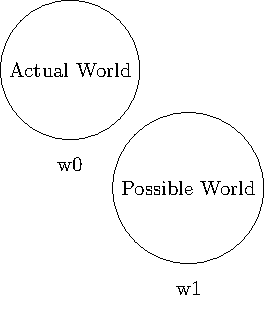
\includegraphics[keepaspectratio]{_main_files/figure-latex/unnamed-chunk-1-1.pdf}}

One way to understand this question, is to consider that for a given fictional utterance, what it infers is that for a given world \(w_0\), there has been an utterance that references an alternative world \(w_1\).

\pandocbounded{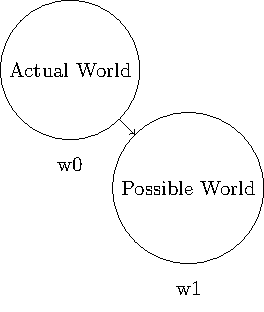
\includegraphics[keepaspectratio]{_main_files/figure-latex/unnamed-chunk-2-1.pdf}}

At alternative \(w_1\), given the speech act, there is some object which is referenced. With fiction, the imagination plays a determining factor in portraying that represented object. The question then becomes, is it the imagination of the creator of the fiction, or the audience? When it comes to moral content in fiction, identifying the object becomes important, what role does the audience perform in determining some content of fiction?

In ``Only Imagine'', Katheleen Stock\footnote{\emph{Only Imagine}.} argues the content of fiction is determined by what the artist reflexively intends the audience to imagine. Here, not only does the artist imagine what is becoming prescribed, but also the audience recognizes what the artist intends for them to imagine. Conversely, Catherine Abell\footnote{{``Reply to {Currie}'s and {Gilmore}'s Comments on {Abell}'s {\emph{Fiction}}.''}} defines intentionalism as a premise which states that an ``actual artist's intentions determine the content of their fictive utterances'' {[}3{]}. Abell argues that fictive utterances are grounded in fiction institutions where an institution is comprised of a set of social practices and rules.\footnote{Francesco Guala, \emph{Understanding Institutions: The Science and Philosophy of Living Together} (Princeton (New Jersey): Princeton university press, 2016); but also E.g., for fiction as an institution see \textbf{carr90?}; Kendall L. Walton, \emph{Mimesis as {Make-Believe}: {On} the {Foundations} of the {Representational Arts}} (Cambridge, (Mass.): Harvard university press, 1990); \textbf{lama94?}; \textbf{smit95?}; \textbf{kopt11?}; \textbf{zipf11?}; \textbf{matr14?}} The rules of fiction institutions enable members of a set of rules to coordinate their communicative practices, etc. Regarding fiction, such coordination is necessary in order to communicate imaginings.

We can imagine having two agents wherein one agent modifies the physical environment of the other. In communicating imaginings, discussants each desire that the other be capable of imagining specific contents prescribed by one of the discussants.\footnote{Abell, {``Reply to {Currie}'s and {Gilmore}'s Comments on {Abell}'s {\emph{Fiction}},''} 30.} Following a set of rules allow the discussants to imagine what the other desires them to do so.

\begin{quote}
Such rules guide agents' actions, and enable them to coordinate on equilibrium solutions to the coordination problem of identifying a medium of exchange, store of value, and unit of accounting.\footnote{Francesco Guala, \emph{Understanding {Institutions}: {The Science} and {Philosophy} of {Living Together}} (Princeton (New Jersey): Princeton university press, 2016), 35.}
\end{quote}

Having the prescribed emotion represents our correct understanding of that fictional utterance. There is an important implication of intentionalism in regards to the philosophy of fiction. The emotions that we experience in response to fiction, unlike those we experience in response to the real world, are not necessarily apt just in case they accord with some moral norm. Rather, an emotional response to fiction is apt if it is the one prescribed by the fiction according to the artist's intentions. The creator of the work makes a fictional utterance to the audience. The fictional utterance is grounded by an artist's intention. Recognizing her audience, the author conforms to the rules and standards of a given community in order to represent an object of emotion to that community.

Here, we may think that the moral activity in the novel is dependent on the author, it rests on the author's intentions. However, the author plays no role in determining who belongs to a given community. She does not determine what objects illicit which emotions in a given community. Although a community can form around a piece of art, the role the artist plays in determining that community is not clear.{[}Look up artistic communities{]}

A similar position is defended by Jonathan Gilmore\footnote{\emph{Apt {Imaginings}}.}. Under this view, the emotional responses that we have in response to fictional objects, are dependent on the creator of that fiction. The dominant view in the epistemology of fiction is \emph{intentionalist} in that ``the fact that we are merely \emph{caused} to feel a given way may be reason to feel that way.''\footnote{Ibid., 132.} For Gilmore, a primary point in favor of the intentionalist view is rooted in a related one. First, how we respond to events represented in art, does not infer how we should or may respond to similar events in the real world. Gilmore then draws a distinction between what is normative, and what is prescriptive regarding our emotional responses to art. One important point here is that what it would be epistemically rational for us to imagine in fictional contexts, is not necessarily applicable in non-fiction.

A known view in psychology of emotions and moral psychology then, argues that emotions are evaluative representative states of things in the real world.\footnote{E.g., see Jonathan Gilmore, \emph{Apt {Imaginings}}; Arnold, \emph{Emotion and {Personality}}; Smith and Lazarus, {``Appraisal {Components}, {Core Relational Themes}, and the {Emotions}''}; Lazarus, {``On the {Primacy} of {Cognition}''}; \textbf{sche01?}; Smith and Lazarus, {``On the {Primacy} of {Cognition},''} to name a few.} If this is true, then we may ask an analogous question, whether emotional responses are also evaluative representative states to fiction as well. Here, Gilmore notes that the evaluation can be apt in either a narrow scope or a broad one.\footnote{Gilmore, \emph{Apt {Imaginings}}, 221} When the creator of a fiction makes a fictional utterance, that utterance is often intended to cause an emotional response in us. That emotional response is a kind of evaluation. In a narrow sense, a given emotion is fitting, for instance when one engages with an immoral work, then one's emotions ought to conform with a successful representation of its contents. Under the broad scope however, one's emotions ought, if one engages with an immoral work, conform with how its contents are successfully represented.\footnote{Gilmore, ibid, 221}

What makes an emotion an apt response to fiction then, is the artist's prescription of that particular emotion via their artwork. Such an emotional state is the appropriate state to have in the fictional context because imagination here plays a functional role. The functional role that imagination here is performing, is to enable an audience to engage with a creative fiction, a fiction which that audience choose to engage with. The creator here seems to anticipate the ability of the audience to invoke the cognitive capacities, e.g.~imagination, important for interpreting fictional utterances. In order to perform the task to which it has been assigned, engage with a given fiction, a prescribed emotion is required. Following this then, we \emph{should} express sympathetic anger when \emph{Rage Against the Machine's} Zack Delarocha pleads for justice assuming that such an emotion is the one prescribed in the context of his plea:

Weapons, not food, not homes, not shoes

Not need, just feed the war, cannibal animal

I walk the corner to the rubble, that used to be a library

Line up to the mind cemetery now

What we don't know keeps the contracts alive and movin'

They don't gotta burn the books, they just remove 'em

While arms warehouses fill as quick as the cells

Rally 'round the family, pockets full of shells

\noindent Perhaps it is not a far cry to argue that Rage prescribes prescribes rage, perhaps anger, in their lyrics given the title they've chosen to give themselves.\footnote{See, Joshua D. Greene, {``The Rise of Moral Cognition,''} \emph{Cognition} 135, no. 0 (2015): 39--42, \url{https://doi.org/10.1016/j.cognition.2014.11.018}.} Further, throughout the years, the band has also heavily criticized various factions of the United States government.\footnote{E.g., see Frank Guan, {``Rage Against the Machine Were 24 Years Too Early''} (Vulture), accessed November 8, 2022, \url{https://www.vulture.com/2016/11/rage-against-the-machine-were-24-years-early.html}.} They have also criticized other governments they believe have fallen short of moral standards they believe to be normative of institutions that have broad influence, coercive and otherwise.

Assuming that a particular emotion is prescribed by the fiction according to the intentions of the artist, the experience of the emotion by the audience represents their correct and apt engagement with the work. Similarly then, we \emph{should} feel sadness when Jay Farrar poetically recounts the historic flooding of Ste. Genevieve MO in Son Volt's \emph{Tear Stained Eye} assuming that this emotion too, is the one prescribed to us:

Seeing traces of the scars that came before

Hitting the pavement still asking for more

When the hours don't move along

Worn out wood and familiar songs

To hear your voice is not enoug

It's more than a shame

But one might think that the emotions we have towards fiction are different in kind from those that we have towards objects in the real world. First, all conscious mental states, according to Gilmore, are intentional states.\footnote{Michael Tye, \emph{Ten {Problems} of {Consciousness} : {A Representational Theory} of the {Phenomenal Mind}}, Representation and {Mind} (Cambridge, Mass: A Bradford Book, 1995), 93--100, \url{https://ezp.slu.edu/login?url=https://search.ebscohost.com/login.aspx?direct=true&db=nlebk&AN=1764&site=eds-live}.} The state represents an object with which that state is directed at.\footnote{``Consider the case of tree rings. Intuitively, the number of rings on a cross section of a tree trunk represents something about the tree, namely, how old it is,'' Tye, \emph{Ten {Problems} of {Consciousness} }, 100.}

Emotions are mental states that represent objects out in the world to us. My fear of a snarling pit bull dog aptly appraises the dog as dangerous.\footnote{Gilmore, \emph{Apt {Imaginings}}, 45.} But \emph{irrational} would be a more accurate description of my fear of chihuahuas.\footnote{For instance see: Joerg Fingerhut and Jesse J Prinz, {``Aesthetic Emotions Reconsidered,''} \emph{The Monist} 103, no. 2 (April 1, 2020): 223--39, \url{https://doi.org/10.1093/monist/onz037}; Klaus R. Scherer, Angela Schorr, and Tom Johnstone, \emph{Appraisal {Processes} in {Emotion} : {Theory}, {Methods}, {Research}}, Series in {Affective Science} (Oxford: Oxford University Press, 2001), \url{https://ezp.slu.edu/login?url=https://search.ebscohost.com/login.aspx?direct=true&db=e000xna&AN=271747&site=ehost-live}. For the relationship between ethics and emotional states, see Darwall, Gibbard, and Railton, {``Toward Fin de Siècle Ethics''}; \textbf{ross19?}; and Justin D'Arms and Daniel Jacobson, {``Sentiment and {Value},''} \emph{Ethics} 110, no. 4 (2000): 722--48, \url{https://doi.org/10.1086/233371}. For the relationship between general evaluations and emotion, see Pascale Willemsen and Kevin Reuter, {``Separating the Evaluative from the Descriptive: {An} Empirical Study of Thick Concepts,''} \emph{Thought: A Journal of Philosophy}, June 1, 2021, 135--46, \url{https://doi.org/10.1002/tht3.488}. Moral evaluation and emotion see: \textbf{mull17?}; \textbf{sche01?}; Ira J. Roseman, Martin S. Spindel, and Paul E. Jose, {``Appraisals of Emotion-Eliciting Events: {Testing} a Theory of Discrete Emotions,''} \emph{Journal of Personality and Social Psychology} 59, no. 5 (November 1990): 899--915, \url{https://doi.org/10.1037/0022-3514.59.5.899},emotional and motivational causation: Arnold, {``Motives as Causes''}.} Therefore some moralist stances place strong value on our emotions.\footnote{See Stephen Darwall, Justin D'Arms, and Daniel Jacobson, \emph{Sentiment and {Value}}, \emph{Ethics}, vol. 110, 4 (The University of Chicago Press, 2000), \url{https://doi.org/10.1086/233371}.} Our emotions constitute appraisals of objects. If it turns out that our emotive appraisal is inaccurate, either we are judging the wrong object, or our judgment is in itself inaccurate. There may be disagreements raised then, when the fictions we consume prescribe amoral emotions, when they evoke emotions that would not be apt in a non-fictive utterance. We laugh at bank robberies when portrayed in some movies though such a response may be inappropriate in real life. On the basis that emotions are evaluative representations of objects out in the world, a question about accuracy begins to emerge. We might think that a mirthful response to a tragedy is not morally justified for instance.

\section{Fictions and Emotions}\label{fictions-and-emotions}

\subsection*{On Emotion}\label{on-emotion}
\addcontentsline{toc}{subsection}{On Emotion}

As we've seen, while it would be epistemically irrational for us to imagine harming others for making an inappropriate comment, this in itself does not entail that it would be epistemically irrational for us to imagine doing so in the context of appreciating the lyrics of a dance song. Following this then, the evaluative norms that govern our emotional responses in the real world, do not govern the emotional responses in fiction. It is important here however, to note that while many moral theories concern the rationality of a given moral action, there are others that do not concern the rationality, but rather, the non-cognitive areas of the mind. The emotion one experiences forms their moral beliefs and values and as such, moral cognition is not cognitive at all.

Unlike traditional moral testimony, art motivates/suggests/represents a given effect in a given context. We can call these evaluative emotions where our emotions are either expressions of our moral judgments, or they motivate our moral judgments.\footnote{Some affective accounts include Gilmore, \emph{Apt {Imaginings}}, 44--84; Jesse J. Prinz, \emph{Gut {Reactions}: {A Perceptual Theory} of the {Emotions}} (Oxford University Press, 2004), 52--78; Prinz, \emph{The {Emotional Construction} of {Morals}}. Also see De Smedt and De Cruz, {``The Epistemic Value of Speculative Fiction''}.} According to the evaluative theory then, our emotions embody evaluation of an object. The loss of a romantic relationship might produce sadness if in the loss of relationship, the subject feels something valuable has been lost\footnote{\textbf{sche01?}} or being chided by one's partner can produce anger.\footnote{Ira J. Roseman, {``Cognitive Determinants of Emotion: {A} Structural Theory,''} \emph{Review of Personality \& Social Psychology} 5 (1984): 14.}\footnote{Arnold, \emph{Memory and the Brain}; collecting 200 written accounts of emotional experiences, argues that emotions are relative to a motivation arising out of a desirable state (stimulus event) that a person wants, e.g.~being praised, or an undesirable state the person does not want, being criticized by one's partner.} A consequence of this view is that two individuals may have differing emotions to the same event. According to this \emph{cognitive} approach, differing perceptions of a similar event are responsible for the discrepant emotional experiences.\footnote{William James, {``What Is an Emotion?''}, 191 for instance argued that emotions are correspondants to processes ``occuring in the motor and sensory centers'', namely ``bodily changes characteristic of emotions {[}which{]} `follow directly the \emph{perception} of the exciting fact'.'' However, James equates the emotion with the bodily response. This approach has been criticized on the basis that bodily response is too slow and undifferentiated to explain discrete emotions (W. B. Cannon, {``The {James-Lange} Theory of Emotions: A Critical Examination and an Alternative Theory.''} \emph{The American Journal of Psychology} 39 (1927): 106--24, \url{https://doi.org/10.2307/1415404}). It should be noted, that following James, Prinz defends the view that emotions are feelings given 1) emotions co-occur with `bodily changes'\,', changes in the body are sufficient to induce emotions, and reduction in bodily ``response reduces emotional experience'' (Jesse J. Prinz, {``Are Emotions Feelings?''} \emph{Journal of Consciousness Studies} 12, no. 8-10 (2005): 9--25).}

Evaluative emotions can be type identified by the evaluative properties they attribute to their objects.\footnote{Gilmore, \emph{Apt {Imaginings}}, 45--46.} A worry arises when we consider our affective responses to fictions that would be considered inappropriate in similar real-world contexts. Is our affective response to these fictions indicative of our moral judgments in similar real-world engagements which these fictions are modeled after? For instance, Currie\footnote{\emph{Imagining and Knowing}.} argues that emotions contribute to our understanding of a fiction by being the right emotion and getting things right in the context of that fiction. Gilmore\footnote{\emph{Apt {Imaginings}}.} argues that this results from a general capacity for practical rationality that allows us to ``richly imagine and emotionally evaluate various courses of potential action'' {[}100{]}.\footnote{Similarly De Smedt and De Cruz, {``The Epistemic Value of Speculative Fiction''} argues that fictions are similar to philosophical thought experiences but that they enable a richer engagement with the contexts by allowing us to experience potential emotions in a way we're prevented from with philosophical thought experiences.} Emotions represent their objects as being a certain way, in the real world but can also be used imaginatively.

One way to understand and answer this question, involves recognizing and defining the criteria for appropriate emotional engagements across real-world and fictional world scenarios. Those who defend continuity argue that these criteria are identical: what is an appropriate emotional engagement to a fictional scenario is also appropriate in the real-world and vice versa. Gilmore\footnote{\emph{Apt {Imaginings}}.}, 131--132 defends discontinuity, namely that the kinds of reasons that we countenance as justifying or challenging our emotions depend on the functions for which our emotions are being elicited. As a result, what is appropriate in fiction and in real life might differ.

What does it say then of someone when they laugh at an inappropriate joke represented in a fiction, film, song lyrics, etc? There are two sides. Continuitists on the one hand think that given our emotional engagements with fictions are modeled after our emotional engagements with real-world states of affairs; we might think that this emotion is justified if and only if the emotion would be a justified response to an analogous object\footnote{For instance, Gilmore, ibid, 1, 102} (the inappropriate joke) in the real world. The question then is whether we \emph{can} represent morally expressive emotions in fictions given this particular discontinuity. Martha Nussbaum\footnote{{``Commentary on {Mourelatos},''} \emph{Proceedings of the Boston Area Colloquium of Ancient Philosophy} 2, no. 1 (1986): 195--207.}; Nussbaum\footnote{\emph{"{Finely Aware} and {Richly Responsible}"}.}; Martha Nussbaum\footnote{{``14 {Non-Relative Virtues},''} in \emph{Moral {Relativism}: {A Reader}}, ed. Paul K. Moser and Thomas L. Carson (Oxford University Press, 2001), 199.};;\footnote{\textbf{stum10a?}} and Zagzebski\footnote{\emph{Exemplarist {Moral Theory}}.} suggest that such representations are necessarily complex depictions of a relationship between two or more individuals, wherein a morally significant emotion is experienced by one or more parties. Therefore although it is plausible, it is not necessarily the case that emotional responses are continuious between fiction and the real world because the intention of individuals such as Henry James specifically is to create such moral complexities as a way of mirroring real life. As such, we might think it warranted that an emotional response to such works will mirror an emotional response in similar contexts in the real world but this says nothing about the intentions of every artist.

The above view would neglect other reasons which would justify an affective response to a work of art. According to the current approach, fiction and other imagination directed emotions are oriented towards other ends---pleasure, entertainment, and absorption---that are justified for different reasons.\footnote{Gilmore, \emph{Apt {Imaginings}}, 132.} Currie\footnote{\emph{Imagining and Knowing}.} argues emotions are not continuous because the objects in fictions are not real {[}62{]}. While it may be true that the Prosecutor Garrison in \emph{JFK} was a prosecutor in real life, the Prosecutor Garrison as \emph{represented} in \emph{JFK} as ``devoted to the truth'' is not a real person. Perhaps Oliver Stone's intentions here are to elicit our admiration towards of Garrison whereas in real life we may have been hard-pressed to do so.

\begin{quote}
For the rational norms governing beliefs do not speak directly to their contents in isolation, but rather to the reasons in favor of their formation or retirement, and to their relations---such as their consistency---while they are held.\footnote{Gilmore, \emph{Apt {Imaginings}}, 152.}
\end{quote}

One particular reason why this is important, has to do with moral education, motivation and the like.\footnote{Maybe we can imagine a community that as a rule does not treat art as containing significant, or any at all, moral motivation. As such, art in such a community just is treated and evaluated for its purely aesthetic, or entertainment, or absorptive qualities.} How do we learn compassionate or empathic behaviors? Some continuitists argue, for instance, that narratives can uncover the good qualities of an individual better than analytic philosophical distinctions. They think that those qualities which make good characters good, e.g.~underlying thoughts and motivations, and features about them that make us want to be better, can only be uncovered through fictional and non-fictional narrative.\footnote{Stump, \emph{Wandering in {Darkness}}, 36, 40--42; Zagzebski, \emph{Exemplarist {Moral Theory}}, 18; ibid., 170.}\footnote{``Putting things this way allows us to see how the emotions can be genuine and not simply playacting, and also how they can have the cognitive content of the real-life emotion'' Nussbaum, {``14 {Non-Relative Virtues}''}, 245.} Upon this, we ourselves then become motivated to act in ways which gave rise to these positive affective states in us.

It is not the response that is unjustified, but rather the decision to engage with that work of fiction if our ends do not cohere with those of the artist.

What we are looking for here I think, are not only constraints that are imposed on what we imagine and how we imagine it, such as would justify laughing at an inappropriate joke, but constraints which would justify creating or consuming such content. Discontinuity as articulated above threatens our ability to say anything other than: if you don't like it don't watch it.

I articulate an approach to this problem. I suggest that the objects which the continuitists and the discontinuitists are concerned with, differ in kind. As such, the point of reference each identifies as the objects of concern in fiction, are not the same. Lastly I argue that the difference is not the content \emph{per se}, but the character of the individual which is expressed through their intention to create.

However, there is a worry about whether entertainment can ever adequately justify all emotional responses in this way. We have emotional responses to things that don't exist. (Fielding 1750/1999, 611--613). First, we may think that our emotions are evaluative analogously to our beliefs. The question that remains is how should we characterize these emotions as opposed to other ones (For instance see Radford 1975). For instance, Nussbaum defends a cognitive view where our emotions are appraisals or value judgments, which ascribe to things and persons ``outside the person's own control'' great importance for that person's own flourishing.\footnote{Nussbaum, {``Symposium on {Amartya Sen}'s Philosophy,''} 4.}\footnote{For other cognitivist theories, see; \textbf{solo93?}; \textbf{lyon80?}; Anthony Kenny, \emph{Action, Emotion, and Will} (London ; New York: Routledge, 2003); Robert Morris Gordon, \emph{The Structure of Emotions: Investigations in Cognitive Philosophy}, Cambridge Studies in Philosophy (Cambridge New York Port Chester {[}etc.{]}: Cambridge university press, 1990); Lazarus, {``On the {Primacy} of {Cognition}''}; Lazarus, \emph{Emotion and Adaptation}.} Here, our emotions are ``intelligent responses to the perception of value,'' and ``they are suffused with intelligence and discernment.''\footnote{Nussbaum, {``Symposium on {Amartya Sen}'s Philosophy,''} 2.} Our emotions here are \emph{about} something, they constitute a special relationship between moral properties and emotion.\footnote{E.g. \textbf{prin010?}} Gilmore adopts the \emph{intentionalist} view in the epistemology of fiction. His intentionalist view is grounded in a dominant view in cognitive theory of imagination where the functional roles of imagination is a determining factor in understanding the contents of fictive utterances.\footnote{Also see Catherine Abell, {``Reply to {Currie}'s and {Gilmore}'s Comments on {Abell}'s {\emph{Fiction}}''} and Chalmers 2002}

\subsubsection*{Cognitive Judgments}\label{cognitive-judgments}
\addcontentsline{toc}{subsubsection}{Cognitive Judgments}

According to cognitivists, to have an emotion involves ``some kind of cognitive judgment.''\footnote{See Nussbaum, {``Symposium on {Amartya Sen}'s Philosophy''}; and Darwall, Gibbard, and Railton, {``Toward Fin de Siècle Ethics,''} 148.} Because emotions shape the landscape of our mental and social lives, a theoretical account of emotions will have large consequences for theories of practical reason, normative ethics, the relationship between ethics and aesthetics, and political thought. In other words, understanding the relationship between emotions and various conceptions of the human good will inform our deliberations as we ask how politics might support human flourishing.\footnote{Nussbaum, {``Symposium on {Amartya Sen}'s Philosophy''}, page num}

Our emotions in response to fiction might also shape our mental and social lives. However Gilmore denies the above arguing that our emotions as directed at fictions, and those we have directed towards the real world, are asymmetric principally because they have a different direction of fit than, say, belief. For instance, we might ask when our emotions constitute such evaluations. Many creatures that are capable of emotions, including babies experience emotion without possessing the concepts which the cognitivist associates with them.

Moral properties can be related to emotion in a number of ways. There might be an essential relation where there is something like a human faculty capable of contributing to our ability to perceive moral qualities. John McDowell and David Wiggins have defended such views that have ``drawn inspiration from the idea that normative or evaluative judgments might bear some analogy with judgments of secondary qualities, or other judgments essentially tied to the exercise of certain human sensibilities.''\footnote{Darwall, Gibbard, and Railton, {``Toward Fin de Siècle Ethics,''} 152.}\footnote{Also see John McDowell, {``Values and {Secondary Qualities},''} in \emph{Morality and {Objectivity}}, ed. Ted Honderich (Routledge, 1985), 110--29; JOHN McDOWELL, {``{PROJECTION AND TRUTH IN ETHICS},''} \emph{University of Kansas}, The {Lindley Lecture}, 1987, 20; David Wiggins, \emph{Truth, {Invention}, and the {Meaning} of {Life}} (British Academy, 1976).} Notice however that this is different from saying that emotions are related to moral \emph{concepts}.\footnote{See Prinz, \emph{The {Emotional Construction} of {Morals}}, 16} On this view, to suggest that there is a relation between our emotions and moral properties is to state a thesis about ``our capacity to grasp moral properties in a standard way.''\footnote{Ibid., 69:16.}

Here, moral judgments are saturated with sentiment. Our moral judgments concern concepts that we care deeply about. Otherwise known as values, these concepts evoke our passions in ways that for instance, are not evoked in relation to whether Honda or Toyota sold more SUVs in a given year. Nussbaum then, defends a theory of emotion wherein emotions are a kind of judgment and in this way, our negative emotion upon witnessing the flooding of Saint Genevieve, say you find us weeping, is a judgment that this particular flood---perhaps not unlike all floods---is bad which says something about what we value as individuals.\footnote{See Nussbaum, {``Symposium on {Amartya Sen}'s Philosophy''}, 17} But this does not necessarily mean that our emotional states are dependent on our cognitive states.

But it isn't necessary that our emotions do correspond with our cognitive judgments.\footnote{De Smedt and De Cruz, {``The Epistemic Value of Speculative Fiction,''} find page.} First, humans have a unique ability to anticipate future events, foreseeing possible outcomes, remember autobiographical events, simulate the future, conceive the viewpoints of others and imagine hypothetical scenarios {[}Gilbert and Wilson 2009; Buckner and Carroll 2007; also De Smedt and De Cruz\footnote{Ibid.}, 2{]}.

It is cognitive abilities such as counterfactual thinking, envisioning the near and distant future, imagining hitherto unfamiliar scenarios which afford us the ability to be ``transported'' into a fiction {[}Richard Gerrig 1993; De Smedt and De Cruz\footnote{Ibid.}, 4{]}. Here, an audience is drawn into and fully immersed within a fictional world. The audience is able to set aside their own cognitive judgments usually accompanying their emotional experiences.

So one aspect of the current concern is that lyrics by groups such as rage against the machine or KRS One are really just entertainment and nothing more. That there is nothing by way of moral knowledge, for instance, that could be derived from them. On this view, art is amoral and accordingly, our emotional responses to art also, are amoral, devoid of any moral worth.\footnote{A theory of evaluative emotions has roots in \emph{representative appraisal theories} which include Arnold, \emph{Emotion and {Personality}}; Smith and Lazarus, {``Appraisal {Components}, {Core Relational Themes}, and the {Emotions}''}; \textbf{smit85?}; \textbf{sche01?}; Smith and Lazarus, {``On the {Primacy} of {Cognition}''}. I have not yet said much about the relation between our evaluative emotions and fiction, though I will devote considerable space to this further down.} As such, our efforts at appreciating the moral arguments made in the art of Rage Against the Machine for instance, is undermined.

However there can be two functions related to this ability. On the one hand, such abilities enable us to better understand implications of a potential action, or what might have happened on the basis of some antecedent event.\footnote{Ruth M. J. Byrne, {``Mental Models and Counterfactual Thoughts about What Might Have Been,''} \emph{Trends in Cognitive Sciences} 6, no. 10 (October 1, 2002): 426--31, \url{https://doi.org/10.1016/S1364-6613(02)01974-5}.} Similarly, our emotions are another type of representation for antecedent events. How would I, or would have felt were \emph{Red} a song about my previous or future relationship instead of Taylor Swift's? Here, fictions are another, more robust form of philosophical thought experience.

This is important because some prominent sentimentalist accounts\footnote{There are two varying sentimentalist views under consideration here. There is what I will call the traditional sentimentalist view defended by Michael Slote \textbf{slot10?}; \textbf{slot07?}. Also see Gelfand, {``Hutchesonian Inspired Agent-Based Virtue Ethics''} and Scott D. Gelfand, {``The {Ethics} of {Care} and ({Capital}?) {Punishment},''} \emph{Law and Philosophy} 23, no. 6 (2004): 593--614, \url{http://www.jstor.org/stable/4150558} among others Some especially prominent defenses of the traditional view include Francis Hutcheson; David Hume; Earl of Shaftesbury. For more recent sentimentalist views, see Darwall, Gibbard, and Railton, {``Toward Fin de Siècle Ethics''}; McDowell, {``Values and {Secondary Qualities}''}; David Wiggins, \emph{A Sensible Subjectivism} (Oxford: Oxford University Press, 1987). Then there is the version I will build from the above quote by Martha Nussbaum above. I will explain this further on.} have argued that for a work of art to engage sufficiently with moral issues, what is needed is a similarly complex, or refined literary engagement. But they might suspect then, that \emph{Tear Stained Eye} is not meant to evoke the emotional state apt for such an event as the 1993 Ste. Genevieve flood. Perhaps it is not necessarily the case that our moral emotions are justified in the same way as they would be were we to witness Saint Genevieve's flooding in person because fiction has more complex aims than this only. Upon witnessing the 1994 flooding of Saint Genevieve, we might appreciate the gravity of the situation responding with emotion that expresses our recognition of the damage which occurs as a result. We may feel distress, compassion, fear, etc. But this does not necessarily suggest that popular songs can be complex in the way needed to evoke the right sorts of moral judgments.

\subsubsection*{Same Emotion}\label{same-emotion}
\addcontentsline{toc}{subsubsection}{Same Emotion}

When speaking about emotions, the emotions that are elicited by fictions are the same as those elicited by actual events. But on one hand we should think that if our emotions are expressions of what we find value in, then why do we not experience those emotions that express our value judgments in fictional{[}b{]} contexts which are analogous to those we experience in the real world?

{[}Explain emotion and cognitive judgment, for instance emotion as a cognitive judgment cannot explain emotions in babies or animals, then explain why, despite the empirical research, why Gilmore thinks they are asymmetric; emotion as sense perception; emotion and quasi emotion, according to dominant theories in neuroscience, our emotions reflecting objects in the real world, are brought about by the same cognitive functions as the emotions we have in response to fiction{]}

This does not specifically state what direction the relation runs in. On one hand, it may be that to say \emph{flooding is bad} is to state a value judgment wherein we give a negative evaluation of the state of affairs in which Saint Genevieve is flooded. It would be odd for someone to laugh while looking at images of a family sitting on the rooftop of their flooded home. However, there is a question that though \emph{Saint Genevieve flooding is bad} is true, that it is only true in virtue of our own judgment and values, a response not necessarily apt towards fiction.\footnote{See \textbf{putn80?}} While I might perceive a news report of Saint Genevieve flooding as negatively valenced, it is not necessary to perceive a fictional report of the same nature similarly. Another option is to say that in stating flooding is bad, we are merely expressing our emotion regarding our perception of actual floods but not necessarily fictional ones.

If our emotional responses contain value and importance in the same way that our other perceptual responses might, then they are necessary for accounts of ethical judgment. But this presents a problem because I might perceive the flooding of Saint Genevieve as bad, but I might perceive the account of the flooding as expressed through Son Volt's ``Tear Stained Eye'' as something other than bad. As such, while I may perceive actual accounts of flooding as bad, it is also possible that I perceive narrated accounts of flooding as something other than bad.

As noted here; emotions are often thought of as complex in regards to human cognition. When considering the relationship between our emotions and our beliefs, it is not often clear that first, there is not such a relationship, but at the same time, it is not clear what this relationship would be if there were such a thing. Perhaps we should view emotions as part and parcel of the system of ethical reasoning. The alternative is viewing morality as a system of principles to be grasped by the detached intellect. Accordingly, emotions would be motivations that either support or subvert our choice to act according to principle. While perceiving accounts of actual flooding, I may reach for and grab sandbags, warn others, call for help etc, when perceiving narrated accounts of flooding, I may instead reflect back on what it must have been like to live through such flooding.

A standard inference of the view, and perhaps this is an answer to the above question, requires only that we think of the complexity or subtlety afforded to fiction as represented in high art. Here, emotions are a ``prominent part of the subject matter of moral philosophy and developing an adequate ethical theory will be to develop an adequate theory of the emotions. Though a big cultural source of emotion is music, typically only high art, including music, is discussed as having a strong relationship between a song and the moral emotions that it expresses. If we think that a reason for this emerges from the insistence of the artist to express such moral emotion, imparting intention into moral kind fiction, then perhaps this is a view defended by Jonathan Gilmore\footnote{\emph{Apt {Imaginings}}.}. On it, we are justified in imagining that some moral judgment is fictionally true just in case our reasons for imagining such is in favor of their formation.\footnote{It is not the case that ``a defender of continuity might say: if it's true in the fiction that, e.g., FAgin is morally corrupt, the beautiful person is intelligent and honest, the mobster's ends are merited . . . then that justifies imagining such things as true'' but rather ``the rational norms governing beliefs do not speak directly to their contents in isolation, but rather to the reasons in favor of their formation or retirement, and to their relations---such as their consistency---while they are held'' (ibid., 151--52). I will look at the continuity/discontinuity distinction further below.} For instance, watching \emph{American History X} requires that we take on the emotional perspective of a impoverished but violent neo-Nazi and his impressionable younger sibling in order to understand the redemption he experienced by both at the end of the movie.

The worry that emerges is that though moral justification then becomes unavailable, only in response to low art does it do so. But this also undermines arguments which attempt to make a connection between low art and moral \emph{unknowledge}.\footnote{Later I will discuss the term \emph{unknowledge} following McGrath, \emph{Moral {Knowledge}}, 172---191, in greater detail in the next chapter.} Emotional aptness is only a question involving high fiction but not low fiction, including those found in popular country and rap songs, television shows, and children's books, for example. Accordingly then, it may be argued that such objects are devoid of moral worth. This would mean then that arguments regarding injustice as found in the popular song ``Wake Up''\footnote{For more on the social significance inherent in RATM's lyrics, see Greene, {``The Rise of Moral Cognition''}.}:

Fist in the air in the land of hypocrisy

Movements come and movements go

Leaders speak, movements cease when their heads are flown

'Cause all these punks got bullets in their heads

Departments of police, (What!) the judges (What!), the feds

Networks at work, keeping people calm

You know they went after King when he spoke out on Vietnam

He turned the power to the have-nots

And then came the shot

\noindent *are* mere entertainment and devoid of moral worth.\footnote{It should be noted that resistance to this conclusion. For instance see; Sue Campbell, {``Being {Dismissed}: {The Politics} of {Emotional Expression},''} \emph{Hypatia} 9, no. 3 (1994): 46--65, \url{https://www.jstor.org/stable/3810188}; Neta C. Crawford, {``The Passion of World Politics: Propositions on Emotion and Emotional Relationships,''} \emph{International Security} 24, no. 4 (2000): 116--56, \url{https://www.jstor.org/stable/2539317}; Greene, {``The Rise of Moral Cognition''}; \textbf{thie00?}.}

Therefore, in the remainder of this chapter and the next, a primary focus will consist of the relationship between popular fiction and moral knowledge. Rejecting the common rationalist charge in twentieth century philosophy, I will first defend a view about the relationship between our emotions and our cognitive states, in regards to moral judgment. I will not only be assuming such a connection, but I will also defend such. The next part will be a focus on the importance of fiction in such a relationship.

\subsection*{Fictions and Imaginations}\label{fictions-and-imaginations}
\addcontentsline{toc}{subsection}{Fictions and Imaginations}

While we might think that the intentions of the art provide a sort of restraint on our imaginings in fiction, fictions also employ various constraints. For instance, what we imagine and how we imagine it when we adopt a particular mental attitude, such as belief, towards what we hold to be true in a story and what we determine to be true in a story depends on the internal and external sources of truth that we recognize as relevant to that story. Gilmore argues that it is not only the intentions of the artist that provide constraints on what is imagined, but that the artist uses internal and external sources to constrain our imaginings.

In order to understand what makes an emotion apt in regards to fiction, depends in part on the answer to the question about imaginings constraints in fiction. What's important here is that we have emotional responses to things that don't exist\footnote{For instance see Henry Fielding, \emph{The {History} of {Tom Jones}: {A} Foundling}, Wordsworth {Classics} (Hertfordshire: Wordsworth Classics, 1999), 611--13.} How should we characterize these emotions {[}See Radford 1975{]}? One way to do so is by trying to understand the functional roles of the emotional states involved {[}Chalmers 2002{]}.\footnote{Imagining and conceiving 2 different things (Peacocke 1985). No univocal explanatory concept (Amy Kind 2013)}

An emotionally apt response to fiction requires that the audience's emotional response is the one called for by the artist {[}Gilmore\footnote{\emph{Apt {Imaginings}}.}; 102--133{]}. This is because imaginings can be ``type-identified'' by their functional roles. The appearance of an object can be a consequence of how I choose to represent that object to myself. The factors such as context become important in cases of imagining, but these factors are largely important by choice. But what follows then, is that the aptness of my emotions evoked by Rage Against the Machine would be appropriate assuming that the agent's anger is the response intended by the agent and assuming that we want to engage with the work as the artist intends. When we respond emotionally to the fate of characters in fictional narratives, we allow ourselves to be ``carried along'' emotionally by the story, and we seem to do this more than we would if the narrative were not a work of fiction.\footnote{Peter Goldie, {``Narrative and {Perspective}; {Values} and {Appropriate Emotions},''} in \emph{Philosophy and the {Emotions}}, ed. Anthony Hatzimoysis, 1st ed. (Cambridge University Press, 2003), 60, \url{https://doi.org/10.1017/CBO9780511550270.013}.}

There are various views as to how to identify imaginings. On one view, imaginings, like other mental states such as belief, can be \emph{type-identified} ``in virtue of their functional role.''\footnote{Gilmore, \emph{Apt {Imaginings}}, 170.}\footnote{Also see Walton, \emph{Mimesis as {Make-Believe}}; Alan Leslie, {``Pretense and {Representation}: {The Origins} of "{Theory} of {Mind}",''} \emph{Psychological Review} 94 (October 1, 1987): 412--26, \url{https://doi.org/10.1037//0033-295X.94.4.412}; Robert M. Gordon, {``Folk Psychology as Simulation,''} \emph{Mind \& Language} 1, no. 2 (1986): 158--71, \url{https://doi.org/10.1111/j.1468-0017.1986.tb00324.x}; Alvin I. Goldman, \emph{Liaisons: Philosophy Meets the Cognitive and Social Sciences} (Cambridge, Mass: MIT Press, 1992); Paul L. Harris, \emph{The {Work} of the {Imagination}}, Understanding {Children}'s {Worlds} (Oxford, UK ; Malden, Mass: Blackwell Publishers, 2000); Gregory Currie, {``Imagination as Motivation,''} \emph{Proceedings of the Aristotelian Society} 102, no. 3 (2002): 201--16, \url{https://doi.org/10.1111/j.0066-7372.2003.00050.x}; \textbf{nich00?}.} However, it is not clear specifically what is the functionalist relation between a cognitive theory of imagination and a functionalist theory of mental states. A functionalist is concerned with what mental states are, not how they account for behavior.\footnote{For instance see Block, {``Introduction.''}} On this account, a \emph{particular pain} is a physical state or event.\footnote{Ibid., 28.} However, Gilmore argues that one way to characterize mental states is by ``collecting ordinary folk-psychological observations'' about how a mental state is causally connected to various causes. For instance how might a particular mental state be connected to a particular belief, a desire or a perception.\footnote{Gilmore, \emph{Apt {Imaginings}}, 18.} If the functionalist is concerned with what a mental state is, and not how it accounts for behavior, then one way to understand what it is, is in terms of its causal relationship to ``sensory stimulations, behavioral outputs, and other mental states.''\footnote{E.g. Block, {``Introduction,''} 28; and Gilmore, \emph{Apt {Imaginings}}, 19.} As such, Gilmore argues that there is a set of three standard distinctions important for individuating imaginings from other mental states: i) imaginings are constrained by the will, ii) beliefs, perceptions, and other mental states are ``subject to a constitutive norm of aiming at what is true.''\footnote{Gilmore, \emph{Apt {Imaginings}}, 19.} iii) imaginings are context-dependent, meaning they depend on a particular circumstance that motivates the imagining. As such:

\begin{quote}
the content of a narrative is not just the set of propositions we are solicited to imagine as true when engaging with the work. Rather, that content is constituted by both the facts within a fictional world that are communicated \emph{and} the modes of presentation through which those facts are conveyed.\footnote{Ibid., 42.}
\end{quote}

Therefore it is not necessary that imagination necessarily aim at what is true. Unlike beliefs, imaginings are typically determined by the willing individual. For instance, it is possible that the appearance of an object is a consequence of how I choose to represent that object to myself. When reading a novel, I may choose to represent myself, or perceive, the protagonist as honest or trustworthy. One way this occurs is that the imagining depends on the particular circumstances that motivate the imagining, say I am reading a story where it is required to perceive the protagonist as such in order to understand what is happening in the story. It possible to think of the movie \emph{American History X} as an example of this. At the start of the movie, the audience is made to feel the motivations underlying Edward Norton's character. The death of his father, the feeling that others are immune to moral condemnation while those like himself are unable to escape it.

But if imaginings do not aim at what is true, then it seems that there is a potential worry questioning when an imagining aims at some object. According to the current view, the worry is that imaginings then aim at what is prescribed to be true in a given context. Imaginings then, unlike beliefs and other mental states not only are constitutive of the will, but they are also context-dependent and it is not clear whether these constraints are always co-extensive.

We cannot reduce all instances of imagining in this way. Sometimes imaginings can be indistinguishable from other mental states like belief. There may be no behavioral difference for instance, between my imagining that others owe me rent or the belief that according to the rules of the game monopoly, a certain player owes me a point value that is demonstrated by a fake monetary value.

We can appeal to external vs internal perspectives. I might mourn what happens to Anna Karenina but express indifference when reading a news report on an otherwise analogous real-life event. As Matthew Matthew Kieran and Dominic Lopes, eds.\footnote{\emph{Imagination, {Philosophy} and the {Arts}}, 0th ed. (Routledge, 2003), \url{https://doi.org/10.4324/9780203498644}.} points out, we can imagine a former Roman Catholic now atheist reading reading Emily Waugh's \emph{Brideshead Revisited}. Given her secular conversion, she will deny that morality categorically depends on the commands issued by God. However, she might still respond to the narrative with sympathy, admiration, and awe. In effect, adopting the perspective and external view of the author.\footnote{Also see Goldie, {``Narrative and {Perspective}; {Values} and {Appropriate Emotions},''} 60.}

\subsection*{First thoughts on fiction, imagination and learning and Why does it matter?}\label{first-thoughts-on-fiction-imagination-and-learning-and-why-does-it-matter}
\addcontentsline{toc}{subsection}{First thoughts on fiction, imagination and learning and Why does it matter?}

Nussbaum explains that narrative works include perceptual and expressional terms that seek to represent our own moral frameworks in the real world. Moral knowledge for Nussbaum, is an agent's ability to perceive a ``complex concrete reality in a highly lucid and richly responsive way; it is taking in what \emph{is there} with imagination and feeling''\footnote{Nussbaum, {``Aeschylus and Practical Conflict,''} 521. Emphasis is my own.}

The function of narrative then according to Nussbaum, is practical in that it emphasizes ``the human importance of a fine-tuned responsiveness to complex particular cases and of a willingness to see them as particular and irreducible to general rules.''\footnote{Nussbaum, \emph{"{Finely Aware} and {Richly Responsible}"}, 290.} This function is evident in narratives which have a complex narrative structure, one which evokes in the reader associated moral activities. These moral activities include human emotional responses associated with moral worth. For an artist to recreate a perception as Nussbaum understands it, then means that ``the artists are not free to create simply anything they like. Their obligation is to render reality, precisely and faithfully; in this task they are very much assisted by general principles and by the habits and attachments that are their internalization.''\footnote{Ibid., 524.} As such, here we only have that an artist must remain faithful to normative moral obligations.

However, Gilmore argues that those norms governing our emotional engagements with moral features in the real world are discontinuous with our emotional engagements in fiction. While we might expect a certain set of emotions in response to a given stimulus, in the domain of fiction, our emotional responses are under a different set of criteria. Our emotions are not under the same normative constraints that they are under in the real world.

Some might argue that this is because those objects which act as stimuli in fictions, are not real objects. But, Gilmore's defense denies this. Fiction-directed affective states are real (preserves realism), their fit with their objects is governed by a different set of norms {[}9{]}.\^{}{[}On Quasi-emotions, Walton\footnote{\emph{Mimesis as {Make-Believe}}.}; Gregory Currie and Ian Ravenscroft\footnote{\emph{Recreative Minds: Imagination in Philosophy and Psychology}, vol. 20, 5 (Oxford University Press, 2002).}. Defenses of Continuity: ``The second kind of opponent, more broadly represented among Anglo-American philosophers of art, assumes or defends the correctness of continuity or invariance: the criteria governing the correctness, fittingness, or aptness are the same whether those token mental states are elicited within the context of imagined experiences or genuine engagements with the actual world'' {[}9{]}.\footnote{E.g., Ronald DE SOUSA, {``The {Rationality} of {Emotion},''} \emph{Philosophy and Rhetoric} 22, no. 4 (1987): 302--3; Susan L. Feagin, \emph{Reading with {Feeling}: {The Aesthetics} of {Appreciation}} (Cornell University Press, 1996), \url{https://www.jstor.org/stable/10.7591/j.ctv75d3wd}; \textbf{wils86?}; P Goldie, {``Explaining Expressions of Emotion,''} \emph{Mind} 109, no. 433 (January 1, 2000): 25--38, \url{https://doi.org/10.1093/mind/109.433.25}; Jenefer Robinson, \emph{Deeper Than Reason: Emotion and Its Role in Literature, Music, and Art} (Oxford : New York: Clarendon Press ; Oxford University Press, 2005); \textbf{matr14?}; \textbf{livi97?}; and \textbf{mesk03?}.} As such, descriptive defenses merely distinguish between descriptive and normative continuity. Further, research only supports descriptive accounts, not normative and therefore: ``The functions of our engagements with fictions and other objects of the imagination license a departure in those engagements from real-world affective norms'' {[}10{]}. As such the following assumptions are not grounded by current views:

\begin{remark}
\leavevmode

\begin{enumerate}
\def\labelenumi{\arabic{enumi}.}
\tightlist
\item
  The idea that a person's emotional response to fiction is an unmediated reflection of his or her character and genuine desires
\item
  The thought that stories evoke a reader's responses by giving her reasons for them that would apply in the real world
\item
  The claim that we can learn from a fiction when it provides a simulation of states of affairs that we might encounter in actual experience
\item
  The methodological assumption employed in a wide range of psychological research that scientists can study the nature of emotions by exposing test subjects to acknowledged fictional representations (e.g., short films) in which those emotions are elicited.
\end{enumerate}

\end{remark}

\section{Discontinuous Fictional Objects}\label{discontinuous-fictional-objects}

Rather than considering the aptness or un-aptness of our emotional responses to fiction, it will be important to consider what the objects of such responses are.\footnote{We might think of such objects in the way sensibility theorists do, i.e. Prinz, \emph{The {Emotional Construction} of {Morals}}, esp.~88-89, evoking a John Locke, {``{OF IDENTITY AND DIVERSITY},''} in \emph{An {Essay Concerning Human Understanding}} (London: Eliz. Holt, for Thomas Basset, at the George in Fleet Street, near St. Dunstan's Church., 1690), \url{https://www.uvm.edu/~lderosse/courses/intro/locke_essay.pdf}'ian sensibility. Here, moral properties are like secondary qualities similar to color, etc. Other similar views include Thomas Reid.} One way to do this, is to evoke standard practices involved in gathering evidence which supports beliefs we hold. In addition to inferences we might make, testimony received by us, perception etc, we also rely on our affective responses to relay important information about our environments to us.\footnote{Micheal Tye, \emph{Ten {Problems} of {Consciousness} } defends a strong version of this view: ``It seems to me not implausible to deal with these cases by arguing that insofar as there is any phenomenal or immediately experienced felt quality to the above states, this is due to their being accompanied by sensations or images or feelings that are the real bearers of the phenomenal character. Take away the feelings and experiences that happen to be associated with the above states in particular cases, and there is no phenomenal consciousness left.''} Not only do such affective states merely give us information about the world, but it is plausible that this information comes shrouded in the mysteries of approbation or its negation. I might decline going down a dark alley owing to the apprehension I feel about doing so in the real-world.\footnote{Zagzebski, \emph{Exemplarist {Moral Theory}}; especially 129--154, is one such account whereby we rely on our feelings of admiration to identify which individuals we should want to be like, emulate etc. Such individuals are direct references for moral kind terms where we identify thick concepts such as good, kind etc, via reference to such individuals. Some concerns which may arise with Zagzebski's view, involves her theory that not every member is capable of identifying proper objects of these terms. In such such cases we rely on experts in the same way we rely on experts to identify gold. For literature regarding asymmetries between moral and non-moral testimony and expertise, see \textbf{hopk07?}; \textbf{hill09?}; Enoch, {``A {Defense} of {Moral Deference}''}. Seminal representative appraisal theories include Arnold, \emph{Emotion and {Personality}}; Lazarus, {``On the {Primacy} of {Cognition}''}.} However, responses to our affects towards fiction can differ from those towards their real-life counterparts. To be able to address this question, we need to consider the metaphysical question of truth in fiction. Discussions on truth in fiction were inspired by an influential paper by David David Lewis\footnote{{``{IV}. {TRUTH IN FICTION},''} 1978.}, and more specifically on his reality principle:

Additionally, it will not do well to talk about fiction without first talking about imagination. Typically, I will walk down a dark alley in a major city between the hours of two and four am and feel fear and apprehension. In some fictions, I may experience similar emotions in similar contexts. But my standard emotional responses in the real world are not always indicative of the ones I would experience in a similar fictional context. In some fictions, I am asked to imagine that I possess extraordinary strength and that I have a thirst for justice. In such cases, I would not experience fear but maybe excitement, an emotion that would not be apt in a similar context in the real world.

\begin{quote}
If \(p_{1}, . . . p_{n}\) are the propositions whose fictionality a representation generates directly, another proposition, \(q\), is fictional in it if, and only if, were it the case that \(p_{1}, . . . p_{n}\), it would be the case that \(q\).
\end{quote}

\[\frac{In f, \psi^{1}, . . ., In f, \psi^{n}}{\therefore In f, \phi}\]

According to it, we consider what is true in a fiction by considering a set of truths in the real-world which \emph{would} entail some conclusion \(\phi\) at the real-world.

\pandocbounded{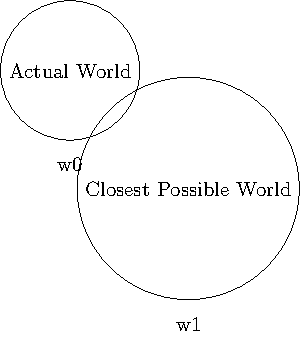
\includegraphics[keepaspectratio]{_main_files/figure-latex/unnamed-chunk-3-1.pdf}}

We then contrast these against the fiction, \emph{Pride and Prejudice} for instance. At \(w_{0}\), the actual world, on the assumption that the actual world is Victorian England, a "a young woman \emph{y}," runs away with "a vicious military officer \emph{o}" prior to marrying. As such, in the real-world as in the fiction, \emph{y's} character is threatened. Therefore there are a number of truths, such as "running away with \emph{o} threatens \emph{y's} character," \(\psi^{1-n}\), which hold at \(w_{0}\), Victorian England, and at least 1 conclusion, \(\phi\) which would hold at \(w_{1}\), \emph{Pride and Prejudice}, on the assumption that these truths also hold and entail the truth of \(\phi\) at \(w_{0}\).

\[\frac{In f, \psi^{1}, . . ., In f, \psi^{n}}{\therefore In f, \phi}\]

\noindent The real-world counterpart is synonymous to

\[\frac{\psi^{1}, . . ., \psi^{n}}{\therefore\phi}\]

\noindent i.e., the real-world where a similar set of facts entail \(\phi\) in the real-world as they do in the fiction.

\section{Imagining Possible Worlds}\label{imagining-possible-worlds}

What the discontinuitists are asking of us, is that we consider additional facts, say \(\omega^{1}, . . ., \omega^{n}\) that entail \(\phi\) in the fiction although they would not similarly do so in real-life.\footnote{"There the fiction presents a character or state affairs as having one property and our response to that property causes us to correctly imagine the presence of another property, even though the two properties bear no genuine real-world explanatory connection" (Gilmore, \emph{Apt {Imaginings}}, 151). Also see Lewis, {``{IV}. {TRUTH IN FICTION}''}.} For instance, a fact such as the artist prescribing mirth rather than the anxiety the audience feels towards the affairs of the military officer and his young lover.

\noindent i.e.,

\[\frac{In f, \psi^{1}, . . ., In f, \psi^{n}}{\therefore In f, \phi} \& \frac{\omega^{1-n} \& \psi^{1-n}}{\therefore\neg\phi}\]

As a mental state, imagination aims at what is true more broadly than other mental states such as belief.\footnote{E.g., see Gilmore, \emph{Apt {Imaginings}}, 18---20.}\footnote{For some useful literature on possible worlds and imagination see, Melvin Fitting and Richard L. Mendelsohn, \emph{First-{Order Modal Logic}}, vol. 480, Synthese {Library} (Cham: Springer International Publishing, 2023), \url{https://doi.org/10.1007/978-3-031-40714-7}; \textbf{scho20?}; \textbf{spau16?} and Amy Kind and Peter Kung, eds., {``Modals and {Modal Epistemology},''} in \emph{Knowledge {Through Imagination}}, 2016, 124--44, \url{https://oxford.universitypressscholarship.com/view/10.1093/acprof:oso/9780198716808.001.0001/acprof-9780198716808-chapter-6}.} First, consider that Imaginings are type identified in virtue of their functional role whereas beliefs by their relationship to their object. If I believe proposition \emph{p}, it will rain tomorrow, I will tend to assert that \emph{p} under appropriate conditions, grab an umbrella before leaving the house; behave in ways appropriate to it being true that \emph{p}; deny what saliently contradicts it; rely on it in inferences; and so on. On the other hand, imagining that \emph{p} is noticeable from believing or desiring that \emph{p}, by typical roles imagining plays in the causal networks connecting sensory inputs, our other kinds of mental representations, and our behavior.\footnote{Gilmore, \emph{Apt {Imaginings}}, 18.}

In other words, unlike beliefs, imaginings are not constrained by the object, say the affairs of the military officer and his young lover, but by our will or the function of the imagining. For instance, assuming that it a given imagining is propositional. Beliefs are counter-factually dependent on the object and tend to change involuntarily with changes in the object whereas imaginings can be a consequence of how I choose to represent it to myself. Not constrained by what is true and is context dependent.

Importantly, this is not to say that imagining is wholly dependent on my will, and accordingly, fictions provide constraints on our imaginations in at least 3 ways, and count in our evaluation of an affective response as appropriate in the context:

\begin{remark}
\leavevmode

\begin{enumerate}
\def\labelenumi{\arabic{enumi}.}
\tightlist
\item
  Through our identification of a story's genre.
\item
  Awareness of the author's communicative intentions.
\item
  My ends as a consumer of fiction.
\end{enumerate}

\end{remark}

\noindent Therefore while beliefs aim at what is true, imaginings aim at what is true in a fiction in pursuit of these three aims.\footnote{". . . a defender of continuity might say: if it's true in the fiction that, e.g., Fagin is morally corrupt, the beautiful person is intelligent and honest, the mobster's ends are merited, and so on, then that justifies imagining such things as true. \emph{Whatever} the means might happen to be that such fictional truths are conveyed to us, they are fictional truths and therefore we are justified in imagining them as such" (ibid., 153). Also see Walton, \emph{Mimesis as {Make-Believe}}, 41; and Lewis, {``{IV}. {TRUTH IN FICTION}''}.}

One concern with regard to apt affective responses with which the continuitists are concerned with, is whether having relevant emotions in a given context is constitutive of a good, or well-lived life.\footnote{Nussbaum, {``Commentary on {Mourelatos}''}, 343--344 argues concerns of human excellence as understood by Aristotle are questions about human value which are expressed in the mutual activities, feelings, and awareness that characterize loving relationships between individuals. A part of the concern here is whether someone can exemplify such excellences and still be moved to express feelings towards even fictional objects which are intended to represent relational objects.} Is the life of an individual who has apt emotional responses in the right contexts, a universally desirable one? If it is, then the imaginative constraints that the continuitists may focus on here is 3, my ends as a consumer of fiction. The moral answer involves feeling appropriate emotions at opportune moments and my questions are what facilitates these or hinders them. Rather than addressing this question however, it will be more helpful to model a way in which such relationships in literature may be expressed. Such relationships are between:

\begin{remark}
\leavevmode

\begin{enumerate}
\def\labelenumi{\arabic{enumi}.}
\tightlist
\item
  Subjects
\item
  Objects of a subject's affects
\end{enumerate}

\end{remark}

\noindent and whether such relations align with my own ends. In other words, rather than considering the object and the ends for which affects are being elicited, the continuitist first considers the aims and pursuits of the perceiver.

Regarding 1, we have a moral character, where I define a moral character as an entity capable of moral perceptions as a response condition to a given context. For instance, see Audi\footnote{{``Moral {Perception} and {Moral Knowledge}.''}}.\footnote{For some important criticism, see Jonathan Dancy, {``Moral {Perception},''} \emph{Proceedings of the Aristotelian Society, Supplementary Volumes} 84 (2010): 99--117, \url{https://www.jstor.org/stable/40927013}.}

\begin{quote}
We can see a theft, hear a lie, and feel a stabbing. But can we also perceive the moral wrongs these acts may entail?
\end{quote}

\section{World Semantic Antics}\label{world-semantic-antics}

According to Audi\footnote{{``Moral {Perception} and {Moral Knowledge}.''}}\footnote{p.~79} we can perceive morality where Audi defines perception in that some perceived properties of an object causally "produces or sustains, in the right way, an appropriate phenomenal representation of it".\footnote{Audi, {``Moral {Perception} and {Moral Knowledge},''} 84.} Such perceptions are of moral characteristics such as \emph{honesty}, \emph{trustworthiness}, etc.

I argue that in cases of narrative, we can perceive some moral characteristic, \(c\), for instance lack of ambition in the husband of Flaubert's \emph{Madame Bovary}. This may be some individual character trait, a personal principle etc. Such traits can be perceived by entities that are capable of moral perception \(Pm\), the narrative's characters or its audience.\footnote{"\textquotesingle This tone at last was right\textquotesingle: that is, if he had said the same words in a different tone of voice, less controlled, more stricken, less accepting, the whole \emph{rightness} of the act, of his entire pattern of action here, would have been undone" (Nussbaum, {``Commentary on {Mourelatos},''} 523, emphasis mine).} These I will call moral characters.

Regarding characters, we can typify such by their ability to perceive, via sentiment or emotion, in relation to some context "lack of ambition in one's partner" for instance. For the most part, these are human relationships. As such, not only are we concerned with the objects of perception, and the intent of the creator of those objects, but in line with our own purposes for engagement, we also care about the character of the one doing the perceiving, who we want to become.\footnote{Zagzebski, \emph{Exemplarist {Moral Theory}}, 129--155; defends an account of emulation whereby we naturally seek to imitate those we admire. As already mentioned, I am not defending this particular claim but rather I hope to model the relevant considerations of fiction which are central to the debate.} What are \emph{their} aims?

Looking at a narrative of a potential world, say \emph{\(w^1\)} then, should reveal a context wherein a character \(c\) perceives a particular characteristic \(Pm\) at \emph{\(w^1\)}. Understanding the context wherein \emph{cPm} is actuated in the narrative \(cPm_{w^{1}}\), means needing to understand the sentiment or emotion of a character expressed as a response condition to some context \(P\), say a theft, murder, or betrayal and any moral judgment \(m\) which arises in them in response.

Narratives identify such relations and as such, a narrative represents a possible world \(w^1\) where \(cPm\) at \(w^1\). Next, we should also consider our own affects, as moral agents \(cPm^{2}\), namely the way I might respond to my response. For instance, looking back at my uncharacteristic calmness while being robbed, I might find my seeming lack of fear surprising. Therefore, there exists some moral context i.e.~\(\exists w^2\), a world \(w^2\) where some entity \(c\)---you or me for instance---capable of moral perception \(Pm\), perceives moral object \(m\), \(cPm^{2}\) at \(w^0\) where the moral object just is \(cPm_{w^{1}}\). A consideration of the affects of the character to a moral significant scenario.

We then ask, what does this make me \emph{feel}. In other words, \(cPm^{2}\). What is our own reaction upon \(cPm_{w^1}\), where \(c\) experiences both sentiment via emotion where sentiment equates to either positive \(+\)~or negative \(-\), i.e.~good or bad, and emotion is either \(Hm\) or \(\neg Hm\), say Happiness or its negation. Here we generalize \(( Hm  \lor \neg  Hm)\) to \(Sm\); meaning \(( Hm \lor \neg Hm ) \rightarrow Sm\). Any expressed emotion, whether negatively or positively valenced, generalizes to \(Sm\). For all worlds under interpretation then, i.e.~\(w^{0+n}\), there exists a world where there exists a person capable of moral perception and moral self-reflection.

\[([cP^{( cPm )_{w^{1}}}] \& Sm)_{w^{2}}\]

In other words;\footnote{They say that a picture is worth a thousand words. These illustrations are merely helpful for conceptualizing possible emotional states in a given context. However, if one wanted to see other modal world illustrations, see Fitting and Mendelsohn, \emph{First-{Order Modal Logic}}; and Saint-Croix, {``Privilege and {Position}''}.}

\[( cPm^{2} \& Sm )_{w^{2}}\]

But what should we do with a fiction that is not blatantly false, but false not only because an author has been forgetful, but because they wish to communicate some additional truth? In other words, why is it not false to say "Holmes wears a silk top hat" in the same way that it would be false to say "Nixon wears a silk top hat" or that it is false that "those lyrics should anger me"?

For instance, Gilmore argues that what determines the appropriateness of an emotional response to a fictional work are the facts that are presented in the work, and the modes of the presentation through which those facts are presented.\footnote{Gilmore, \emph{Apt {Imaginings}}, 42.} Here, our emotions are evaluative appraisals of things both in the real-world and the contents of our imaginations caused by fictions, but in fictions, these evaluations are prescribed.\footnote{Gilmore, \emph{Apt {Imaginings}}, 57. For more on evaluative emotions, or emotions as evaluative appraisals, see Nussbaum, {``Symposium on {Amartya Sen}'s Philosophy''}.}

\noindent The answer to this question we might think is that we must first abstract away from the original to several of the possible revisions that remain closest to the original.\footnote{Lewis, {``{IV}. {TRUTH IN FICTION}''}; also see Gilmore, \emph{Apt {Imaginings}}, 32; and Walton, \emph{Mimesis as {Make-Believe}}, 145.} Gilmore's contribution, is in addition to our abstractions, we also include ours and the author's aims.

While at \(w^{1}\) and \(w^{2}\) it is the case that

\[\psi^{1-n}\therefore\phi\]

\noindent At \(w^{0}\), it might also be the case that

\[\psi^{1-n}\&\omega^{1-n}\therefore\phi\]

\newpage

\noindent Using possible worlds then, \(\exists w^{2}\) such that

\pandocbounded{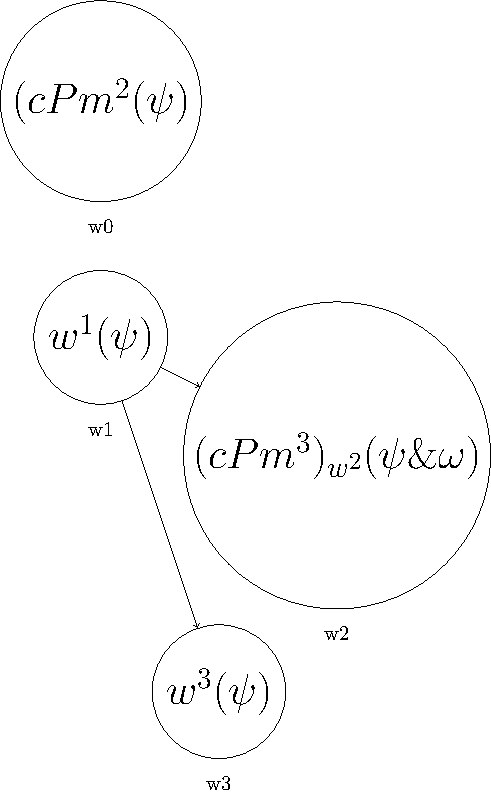
\includegraphics[keepaspectratio]{_main_files/figure-latex/unnamed-chunk-4-1.pdf}}

\noindent *only* potentially accessible to \(w^{0}\) such that

\[( cPm^{2} \& Sm^{2} )\]

\noindent In other words; \[( cPm^{2} \& Sm^{2} )_{w^{2}}\].

The problem I see with this approach, is that the moral worth is in the action of engaging or refraining from engaging with certain art works. However, it is not clear what justifies whether someone engages in a certain work of art or not. In consequence, this does nothing for moving the discussion along. What is missing I think, is that we've ignored the character of the perceiving individual. There are some continuitists who situate moral evaluation in the contexts of caring relationships. What they care about, are the representations of such relationships. Ultimately, we need something in the work that would repel the individual of moral character from the work. There are two types of evaluation, and what repels an audience must be aesthetic. Therefore to explain how the ethical features of a work repels an audience, Gilmore wants to make the moral values synonymous with the aesthetic ones. Therefore, when the function of the work is to realize a morally relevant aim and fails, the failure is aesthetic since it sought to a certain imaginative function but failed. Yet, this does not explain works of art that do not have morally relevant aims, but instead monetary, or entertainment. In the chapters that follow, I address this.

\chapter{Rational Sentiment and Testimony}\label{rational-sentiment-and-testimony}

Morally right action seems to have to do with their relations to other persons and therefore moral testimony is about behaviors directed at others. Striking a rock is typically thought of as an amoral act, unless the rock is an expensive piece of granite that your neighbor intended to install in their kitchen. But when we think about such behaviors, it is not enough that a person has cognitive access of a given proposition about their obligations to others. A firefighter explaining that their motivation for running into a burning building does not usually begin with a recitation of Kant's moral imperative. It is not enough that one has the correct belief about the right course of action towards others. Similarly in epistemology, it is not enough for knowledge, a success condition, that an individual holds the correct belief of a given proposition. Right, in the epistemological sense requires some condition grounded in knowledge. Morally, this sort of epistemological success also invokes a proper oriented sensitivity to other persons as well. This is a success condition that satisfies the demands of moral knowledge. It is often expressed by making reference to certain emotions such as empathy and so on, that rationalize a given behavior. However, there are many concerns that arise when we think of a given emotion as an obligation. We do not often think that we can necessarily convince others the importance of such non-cognitive states as these are not often thought of as under our direct control. We would be hard pressed to lecture our children into being more empathic. One way to first talk about such obligations then, is by thinking of their orientation as prior to reason. Many would think that such talk then is disqualified from philosophical analysis as wisdom is in part a product of reason.

In the last section, I argued that a knowledge first account of justification is an important step towards thinking of apt non-cognitive or affective states as a fundamental obligation. Famously, epistemologists for a long time attempting to understand knowledge as a justified true belief. What this meant is that in order for some person's belief to amount to knowledge, it had to be true, the agent had to believe it, and the person's belief needed to be justified. For instance, if someone lies to me, and in my naivete, I believe them, my belief probably would not be justified. Knowledge first views argue that knowledge is foundational, if we believe that some proposition is true, because we in fact know that it is true, then our belief in that proposition is justified. A small pre-linguistic child who witnesses a mouse run into a hole, knows that they say a mouse run into a hole. On traditional JTB theories of knowledge, the child would likely not be justied, but on the knowledge first model, it would. In this section, I raise questions for theoretical notions of testimony, arguing that moral testimony is different than non-moral because of its ability to connect right action and right reason by facilitating appropriate feeling.

\section{A testimony of normative behavior}\label{a-testimony-of-normative-behavior}

The object of non-moral testimony is to communicate ``that'' something is the case. Non-moral testimony testifies ``that'' the sky is blue, ``that'' 2 + 2 = 4, ``that'' pork is not kosher. Moral testimony is different from non-moral testimony however. The object of moral testimony is not only to communicate ``that'' something is the case. It is not enough to know ``that'' lying is wrong, or ``that'' giving to charity is good. Consider the following vignette:

\begin{quote}
You are on holiday and someone gives you tickets to a boxing match. En route you bump into a friend who asks your plans for the evening. You tell her that you are headed to the stadium though you are not sure where it is. She replies: ``It's on 21st street.'' Taking her to be reliable, you defer to her and head for 21st street. Before parting she asks what you're going to see at the stadium. You tell her that you are going to watch boxing. She replies: ``It's morally wrong to watch boxing.'' Taking her to be reliable, you defer to her and head back to your hotel.\footnote{\textbf{flet16?}}
\end{quote}

Both narratives and testimony are ubiquitous across societies. From telling a loved one how our day at work was, to telling a psychologist why we think no one at work likes us. We use stories to see the moral landscape for what it is. Stories help us to imagine scenarios not only cognitively, but they allow us to feel the effects of betrayal and the pain of loss as if it happened to us. Aeschylus' telling of the tragedy \emph{Agamemnon} tells a story of moral conflict. When \emph{Agamemnon} sacrifices Iphigenia, we feel betrayed.

We often think that moral testimony amounts to, ``you shouldn't \(\phi\)'', ``\(\phi\)-ing is morally wrong'', or that you should \(\psi\) instead. For instance, tell my friend that I will loan him money as soon as he gets his life together.\footnote{Nickel, {``Moral {Testimony} and Its {Authority}.''}} The testifier then gives a number of reasons why one should not \(\phi\). Perhaps he may say, `sexism is wrong,'\footnote{See \textbf{jones99?}} or that unjustified killing is,\footnote{See Julia Driver, {``Autonomy and the {Asymmetry Problem} for {Moral Expertise},''} \emph{Philosophical Studies: An International Journal for Philosophy in the Analytic Tradition} 128, no. 3 (2006): 619--44, \url{https://www.jstor.org/stable/4321738}.} that your friend will only use the money to support his addiction.

\subsection*{Praxis and Right Reason}\label{praxis-and-right-reason}
\addcontentsline{toc}{subsection}{Praxis and Right Reason}

But consider what a good defense of liberal immigration policy does. Assuming that we want to point out that someone has good reasons for immigrating to another country, it is often not enough to state various facts surrounding immigration and reasons for doing so, such as many refugees and other immigrants are seeking a better life, fleeing violence and political persecution. A more effective way to help another see the truth about a given moral claim, including those surrounding the rightness of a liberal immigration policy, is to tell a story that explains why one left their country of origin, family, friends, and even children. For instance, we might begin with something like, on August of last year, John's barn was intentionally set on fire. Shortly there after, he received a envelope from a uniformed police officer, inside were pictures of his sleeping family.

We also use stories to advocate for a change of some kind. A victim may recount what happened to them in the wee hours of the night as a way to introduce a policy suggestion regarding gun restrictions. The victim of police violence may tell a story about being profiled by biased police officers as a way to promote police reform. On the one hand, the victim of police violence could have made a formal argument about the need for police reform. They might argue that violence undermines one's moral autonomy and that one should never undermine another's moral autonomy. Stories are often more effective however. A person will tell their story hoping that their audience can imagine the way they felt at the moment of their victimization. They would hope that their descriptions of a given event, would place their readers into their shoes. I will argue, that these uses of narrative show us that what makes these moral concerns moral, are those important emotions that accompany them. As such, it will be helpful to understand the difference between moral and non-moral testimony as the difference between assertions that convey emotion and those that do not.

What the above suggests, is that we often use narrative as a form of moral testimony. However, we should dispel some concerns. Moral knowledge is nothing like non-moral knowledge. Moral knowledge is concerned with motivation and behavior while non-moral knowledge is merely concerned with behavior. First, lets consider some individual named Sue.

Sue decides to get inoculated against a known virus because she is afraid of becoming sick. However, Sue has never really thought about whether the virus is contagious or not and what this means. Sue does not care much about the virus beyond whether or not it can make her gravely ill.~In fact, if it were ever proven to Sue that because of her age or genetics, she was not susceptible to any illness as a result of this particular virus, she would decline getting the vaccine regardless of how contagious it is, or how serious it is for others. This is because Sue is not at all concerned with the virus' effect on others. There are two different questions here. The question about whether or not a virus is contagious can be a moral question if one worries about the virus' effect on others, say someone who is immunocompromised.

Mary however, is an individual who, while she does not want to become ill as all of us do not want to become ill, has the additional motivation of not wanting to pass an illness to friends and family who may experience significant health effects as a result of getting sick from this virus. While Mary is reasonably assured that were she to catch the virus, it would be no worse than a sniffle or two, she would still receive the vaccine because she does not want other members of her family to become ill.~Mary is concerned with facts about the virus in a way that Sue is not. For Mary, her beliefs about the virus do involve others. As such, her beliefs about the virus are action guiding and grounded in her concern for others. Given that her beliefs about the virus involve its effect on other people, her motivations about the virus are moral.

We can further contrast this against a case wherein though Clarice may reasonably believe that no one in their family would become seriously ill from the virus, she still pursues inoculation because she would feel terrible if \emph{anyone}, whether friend or foe, became seriously ill from catching the virus. Clarice is impartial and so are her moral beliefs. Both Mary and Clarice have an additional motivation that Sue clearly lacks. Both Mary and Clarice get the vaccine because they do not want to spread an illness and would feel really bad if they were the cause of another becoming ill.

If Sue is to ask an expert whether or not she should get inoculated, the expert would have to infer reasons that are important for Sue, but very often, the medical expert assumes that Sue's reasons are moral. Narrative is the best way to facilitate such reasons and as such, narrative can justify a given moral belief. In what follows, I will argue that justification for our moral beliefs are grounded in part, in our concern for others. While it is important to know whether or not someone should get a vaccine based on reasons of prudence, not wanting to experience financial difficulty as a result of missed wages for instance, it is also important to know whether or not someone should get a vaccine based on moral reasons. Namely the effect of their decisions on other people.

Understanding what narrative is and does will give us a better appreciation for why narrative is a form of moral testimony. First, we can begin with the observation that what a person knows about the world depends on evidence, including what they know about the moral world. But there are two kinds of evidence. On one account, critical reflection and reasoning is a kind of evidence whereby an agent's belief counts as knowledge just in case her belief satisfies a number of conditions such as critical reflectivity and equilibrium with held principles, or is justified.

The activity of justifying one's belief, is the activity of an agent identifying a set of judgments she has, `genocide is morally impermissible', `murder is wrong', `one should not plagiarize'. She then attempts to formulate a set of general principles which account for the judgments. She might argue for instance, that murder is wrong because it undermines the autonomy of moral agents. She then attempts to determine whether her principles are compatible with her judgments, recursively modifying each until they are.\footnote{McGrath, \emph{Moral {Knowledge}}, ch.~2; also see Scanlon, \emph{Being Realistic about Reasons}, 76--77.} Therefore, a set of conditions that a belief needs to satisfy to be justified includes critically reflecting on that belief and equilibrium between a held belief and principles it is grounded in.

But there are problems with this account, for one, it does not account for a lot of our knowledge about the world. For instance, we do not need to critically reflect on our beliefs about feeling the sun's rays on our skin to know that the sun is shining. Similarly, we do not need to reflect on the fact that some actions seem morally right while others wrong. However, moral perceptions differ in an important way from non-moral perceptions. They are amenable to change. While it may feel perfectly just to young Mary to deny credence to Sam's testimony given his less than perfect command of the English language, older Mary can look back on her young Mary with regret. Mary has developed moral understanding, and therefore xenophobia no longer feels right to her.

Moral understanding is how we feel about a behavior or action. What we hope to achieve with moral testimony then, is a change in the way someone feels about a given action or behavior. Narrative is an effective method of moral testimony because it is a source of moral understanding. We confer moral worth to a behavior when the agent morally understands why their action was the right one

As we have witnessed with the case of Sue, you can acquire moral knowledge through testimony. Moreover, moral testimony is about action. But there are two ways to understand action in these contexts. Moral testimony can, and often does, correspond to right action. It does not, however, correspond to morally right action; actions that have moral worth.

\section{Acquiring Sensitivity to Morally Right Action}\label{acquiring-sensitivity-to-morally-right-action}

Just what is morally right action? As the literature goes, there is an important connection between moral understanding and good character, namely that moral understanding is a primary component in one's ability to reliably do the right thing.\footnote{\textbf{hill09?}; Nickel, {``Moral {Testimony} and Its {Authority},''} 256; \textbf{mark10?}} But, it is possible for an agent to characteristically perform the right actions for the wrong reasons. An agent may reliably perform some right action because they care about self-image or because of some other non- moral concern\footnote{See Nomy Arpaly, {``Moral {Worth},''} \emph{The Journal of Philosophy} 99, no. 5 (2002): 223--45, \url{https://doi.org/10.2307/3655647} for a defense of this point.} or like Sue through some odd outcome of reason. Morally right action then, must be an action that has moral worth for that agent, not merely any agent who performs that right action. Another agent who acts rightly, perhaps performing those exact actions as the former in analogous situations, may not fare as well with respect to moral worth.

\subsection*{Through Thick and Thin, Two Accounts of Moral Understanding}\label{through-thick-and-thin-two-accounts-of-moral-understanding}
\addcontentsline{toc}{subsection}{Through Thick and Thin, Two Accounts of Moral Understanding}

On the thin view of moral understanding suggested by Alison,\footnote{\textbf{hill09?}} Sue understands that she should get the vaccine (wHs) if she is also able to do the following given the truth of (wHs) {[}102--103{]}.

\begin{Shaded}
\begin{Highlighting}[]

\NormalTok{Reason that \textquotesingle{}If I should should get inoculated, then I should help my neighbors.\textquotesingle{}}
\end{Highlighting}
\end{Shaded}

\begin{Shaded}
\begin{Highlighting}[]

\NormalTok{Follow an explanation of why (wHs) \textquotesingle{}I should should get the vaccine,\textquotesingle{} given by someone else; be able to explain (wHs) in her own words;}
\end{Highlighting}
\end{Shaded}

\begin{Shaded}
\begin{Highlighting}[]

\NormalTok{draw q{-}{-}{-}e.g., we should not hit others{-}{-}{-}from (wHs);}
\end{Highlighting}
\end{Shaded}

\begin{Shaded}
\begin{Highlighting}[]

\NormalTok{draw (wHs)\textquotesingle{}{-}{-}{-}say Bob{-}{-}{-}(or likely (wHs)\textquotesingle{}) from q\textquotesingle{} where (wHs)\textquotesingle{} and q\textquotesingle{} are similar but not identical to (wHs) and q;}
\end{Highlighting}
\end{Shaded}

\begin{Shaded}
\begin{Highlighting}[]

\NormalTok{given information that (wHs), give the right explanation}
\end{Highlighting}
\end{Shaded}

On'\footnote{\textbf{hill09?}}s view, testimony is not sufficient for acquiring moral understanding, but can serve as justification. Some initial reasons why moral understanding is valuable: Moral Understanding is essential to acting well.{[}119{]} On this view, a grasp of reasons might be the only way to perform the right actions reliably.

\begin{quote}
Suppose your reliable friend has told you not to cheat your customers because doing so is unfair. You believe her, but on your own behalf, you cannot really see anything wrong with enriching your share holders at your customer' expense. There is a perfectly good sense in which you know why cheating your customers is wrong: you know that it is unfair. And yet you yourself have not grasped the connection between the wrongness of the action and the reason why it is wrong. So you say to your customers what you were told---citing the unfairness of giving the wrong change as justification for your action---but you cannot give an explanation in your own words, and you cannot reassure customers that under slightly different circumstances, you would treat them well (since you yourself are not able to work out what you would have moral reason to do in those circumstances). Without moral understanding, your ability to participate in the exchange of reasons is necessarily limited.\footnote{\textbf{hill09?}}
\end{quote}

There are two points about the importance of morally worthy action here that we should note. First, it is important because virtue requires justification, namely the ability to justify one's actions. When one performs a morally worthy action, she is able to justify her action to others in a way that explains it to them. Further, in order for an action to be morally worthy, they have to come from a place of good character. So, crucial to moral worthy actions is having good character. ``{[}M{]}oral understanding is essential to good character and to morally worthy action, that is, to right actions performed for the right reasons.''\footnote{\textbf{hill09?}}

\begin{Shaded}
\begin{Highlighting}[]

\NormalTok{Right Action {-}\textgreater{} Actions performed for the right reasons}
\end{Highlighting}
\end{Shaded}

An action is morally right only if it is a right action performed for the right reasons. And moral understanding is crucial to certain kinds of morally worthy action. But this conflates being able to justify your actions, with the moral worth of those actions. Perhaps this is all the study of ethics, say medical ethics is. On such a view, a hospital might hire a team of ethicists to justify their actions rather than leading in critical reasoning about complex medical issues such as patient autonomy.

\subsection*{Knowledge and Understanding}\label{knowledge-and-understanding}
\addcontentsline{toc}{subsection}{Knowledge and Understanding}

Robert\footnote{\textbf{howa18?}} understands Noma'\footnote{\emph{Unprincipled {Virtue}}.}s position as a form of non-cognitive understanding.\footnote{Also see, Arpaly, {``Moral {Worth}.''}} However, he leaves open the possibility that this can be thought of as a form of knowledge. This is a point that deserves further development.

\begin{quote}
Huckleberry Finn befriends Jim, a slave, and helps him escape from slavery. While Huckleberry and Jim are together on a raft used to escape, Huckleberry is plagued by what he calls ``conscience.'' He believes, as everyone in his society ``knows,'' that helping a slave escape amounts to stealing, and stealing is wrong. . . . Like many children (and adults), Huckleberry is not very good at abstract deliberation, and it never occurs to him to doubt what his society considers common sense. Thus, he fails to find a loophole. . . . Having thus deliberated, Huckleberry resolves to turn Jim in, because it is ``the right thing.'' But along comes a perfect opportunity for him to do so, and he finds himself psychologically unable to do it.\footnote{\emph{Unprincipled {Virtue}}, 75; also see Bennett, {``The {Conscience} of {Huckleberry Finn}.''}}
\end{quote}

Jonathan Bennett\footnote{{``The {Conscience} of {Huckleberry Finn}.''}}; and\footnote{\emph{Unprincipled {Virtue}}.} highlight Huckleberry Finn's interaction with Jim as morally worthy despite his lack of moral understanding. There are two ways to understand this failure. First, Finn does lack moral understanding under the traditional view. He reasons from a place of understanding that he should turn Jim in. He knows stealing is wrong and that one has a moral duty to return another's stolen property. But he does not understand where such a rule is applicable. If Finn understood that stealing is wrong, he would know the correct application of this rule, but because he does not understand that stealing is wrong, he falsely believes that not turning Jim in amounts to stealing.

The other way to understand Huck Finn's failure, is that the first relies on an insufficient view of understanding. It is possible that Laura Callahan\footnote{{``Moral {Testimony}.''}}'s view is closer to the second. ``Understanding of this kind might be thought necessary for morally \emph{worthy} action, or for virtue.''\,''\footnote{Ibid., 443.}Many hold that only actions undertaken \emph{for} the reasons that make those actions morally right are morally worthy.'' Merely appreciating some action as being the thing to do will not suffice for moral worth as long as one lacks more direct motivation by the reasons that make the action right.\footnote{Ibid.}\footnote{Also see, e.g.~see Nickel, {``Moral {Testimony} and Its {Authority}''}; and \textbf{mark10?}.}

Finn's failure to turn Jim in is an action we do associate with moral worth and as such, comes from a place of moral understanding. Although it does seem that some form of moral reasoning takes place, in the end it is not connected with Finn's moral action however. Arpaly calls this \emph{inverse akrasia}, doing the right thing against one's better reason or judgment. Finn has reasoned correctly and therefore has moral understanding, but what he understands in the thin way is not the morally correct action. What he does have though is knowledge, and his knowledge is why his action possesses moral worth. As such, moral understanding is connected to the psychological turmoil that Huck Finn experiences resulting in his inability to turn Jim in. However, this leads to some troubling questions. First, what Howard calls non-cognitive understanding, looks more like moral perception. The reaction that Huck has to turning Jim in, resembles the inability that one may have at stepping onto a transparent platform suspended over a large crevice. This person may very well reason to themselves that the platform is safe and has been inspected on numerous occasions by the relevant experts. However, they may not be able to bring themselves to walk onto the platform because of their non-cognitive perception that it would be unsafe to do so.

As noted by Alison,\footnote{\textbf{hill09?}} what we care about regarding moral knowledge is one's behavior, and whether this behavior deserves moral praise. Arpaly argues that understanding as defined by Hills is not as central to moral worth as Hills thinks. But this just means that understanding is not as central not to moral worth, but to behavior. Understanding does not need to be central to behavior because we often theorize on various issues without any intention on acting as the outcome would suggest. Therefore on this view, our affective states are more important for the moral worth of our actions.

\noindent Consider the following claims:

\begin{quote}
What is it to have good character, to have the virtues? \ldots{} In general, someone with a good character is disposed to \emph{feel}, choose and act rightly. {[}\footnote{\textbf{hill09?}}, 108; emphasis mine{]}
\end{quote}

Both\footnote{\textbf{hill09?}} and Robert\footnote{\textbf{hopk07?}} argue that having the right to a moral belief requires grasping the moral grounds for it.\footnote{\textbf{hopk07?}} In Sue's case, it would be right for her to receive the vaccine. However, to say that something is right, is not the same thing as saying that it is \emph{morally right}. Grasping in this sense implies a mental property with motivational content. Paulina Paulina Sliwa\footnote{{``Moral {Understanding} as {Knowing Right} from {Wrong},''} \emph{Ethics} 127, no. 3 (April 2017): 521--52, \url{https://doi.org/10.1086/690011}.} and other optimists (E.g. Enoch\footnote{{``A {Defense} of {Moral Deference}.''}}) point out that the missing piece is not understanding as understood by Hills, but rather a special kind of sensitivity to the moral reasons present in a particular case. This sensitivity confers moral worth onto an agent's action and the sensitivity in question can come by way of moral testimony.

\begin{remark}
Following Hopkins, we can call this the recognition requirement:

The Recognition Requirement** (morally right action is acting for the morally relevant reasons) has to do with action, but it has to do with the part of action that lies within an agent: her psychological and \emph{motivational} makeup. {[}Nickel\footnote{{``Moral {Testimony} and Its {Authority}.''}}, 258; emphasis mine{]}
\end{remark}

The problem with Hills' account then, is that it fails to recognize the important role that moral knowledge, better known as moral perception, plays in moral understanding.

Notice how the primary question is not about whether moral testimony can or can not make moral knowledge available for either view. In cases of moral testimony, we rely on another's moral judgment; maybe we might think someone is in a better epistemic position than ourselves, and we accept a moral claim because that person asserted it. But this does not mean that we do not have knowledge given the way we've come to hold some view. In the following, I begin to tease apart two different senses of ``grasping reasons.''

\section{Understanding Moral Sensitivity}\label{understanding-moral-sensitivity}

Moral judgments require interpersonal justification. Here, an agent's action is a direct response to the moral requirements guiding rational action. Testimony fails to provide adequate reasons for moral action because one's reliance on testimony highlights their inability to respond to the moral requirements present.\footnote{See Nickel, ibid, 256; \textbf{hopk07?}; \textbf{hill09?}, 102.} Pessimists with regard to moral testimony defend the asymmetry thesis of moral testimony in one of two ways. First, though moral testimony can impart moral knowledge, the asymmetry is explained by the fact that we have a duty to exercise our moral conscience, a duty we do not have in non-moral concerns.\footnote{Enoch, {``A {Defense} of {Moral Deference}''}; McGrath, \emph{Moral {Knowledge}}; Jones, {``Second-{Hand Moral Knowledge}''}; Driver, {``Autonomy and the {Asymmetry Problem} for {Moral Expertise}''}; \textbf{hopk07?}; {``The {Conflict Between Authority} and {Autonomy},''} 20--31; Elizabeth Fricker, {``Testimony and {Epistemic Autonomy},''} in \emph{The {Epistemology} of {Testimony}}, ed. Jennifer Lackey and Ernest Sosa, 1st ed. (Oxford University PressOxford, 2006), 225--50, \url{https://doi.org/10.1093/acprof:oso/9780199276011.003.0011}.} But this does not absolve the worry regarding moral sensitivity.

Other defenses reduce moral understanding to something like a capacity for knowledge, where understanding amounts to varying degrees of moral knowledge\footnote{Sliwa, {``Moral {Understanding} as {Knowing Right} from {Wrong}.''}} whether the agent knows \emph{`p'} or not. However, like pessimists, such defenses define understanding as something which is solely cognitive. For instance,;\footnote{\textbf{howa18?}} Callahan\footnote{{``Moral {Testimony}.''}};;\footnote{\textbf{flet16?}} Enoch\footnote{{``A {Defense} of {Moral Deference}.''}} and Sliwa\footnote{{``Moral {Understanding} as {Knowing Right} from {Wrong}.''}} point out that the missing piece is not understanding as understood by Hills, but rather a special kind of cognitive sensitivity to the moral reasons present in a particular case.\footnote{Sliwa, {``In Defense of Moral Testimony''}; Sliwa, {``Moral {Understanding} as {Knowing Right} from {Wrong}.''}} McGrath\footnote{{``The {Puzzle} of {Pure Moral Deference}.''}} defends a view on which there are moral experts, individuals who have a better appreciation or are specially sensitive to at least some moral facts than are others.

A point that isn't addressed in depth in the moral testimony literature, is that in the moral realm, having emotional/motivational states appropriate to one's beliefs is distinctively important. If one, say agent \emph{A} understands a moral proposition, say \(mP\) \emph{is true}, then \(A\) should appreciate the reasons why \(mP\). If \(A\) appreciates why \(mP\), then \(A\) appreciates \(mP \rightarrow \psi\), namely, that if \(mP\), then \(q\).\footnote{Callahan, {``Moral {Testimony},''} 441.}\footnote{Also see Alison \textbf{hill09?}; \textbf{hill13?}; \textbf{hopk07?}; Nickel, {``Moral {Testimony} and Its {Authority}''}. For how this relates to non-moral understanding literature see Stephen R. Grimm, {``The Goal of Explanation,''} \emph{Studies in History and Philosophy of Science Part A}, December 2010, 337--44, \url{https://doi.org/10.1016/j.shpsa.2010.10.006}; Nickel, {``Moral {Testimony} and Its {Authority}''}; and \textbf{hill09?}; Hills, {``Understanding {Why}''}.}. Therefore, ``Having understanding comes with abilities.''\footnote{E.g. see, Alison Hills 2009, 102--103, 2016 and Grimm 2011} Some abilities include being able to ``form additional correct moral beliefs, say \(mP'\) and act rightly in particular, novel situations.''\footnote{Callahan, {``Moral {Testimony},''} 443.} However cognitive reasons are not the only reasons \emph{why} \(mP\) will be true and not the only motivations for an agent's acting from \(mP\).

However, this does not occur in the Huck Finn case. Finn reasons that not returning a runaway slave is akin to stealing. Stealing is wrong. Therefore one should return a runaway slave. When Finn does reason (\(mP \land q\)) \(\rightarrow \psi\) then, the result is not where the praiseworthy relevant features of the action are found. Finn is incapable of \(\psi\)ing and as such, performs a morally worthy action.

Understanding the relevant moral propositions (having the appropriate feelings and motivations) in a situation is sufficient to enable one to act with moral worth in a situation (as long as one also has an accurate, sufficient grasp of relevant non-moral information).\footnote{Ibid., 445.} An agent who has the appropriate feelings and motivations, motivation to act for the right reasons,\footnote{Ibid., 450.} also acts with moral worth. As defended by,\footnote{\textbf{howa18?}} we might think that moral understanding is important for moral motivation. If one will be motivated by the right reasons, then one should have a grasp of the right reasons and the support they provide for the relevant moral judgment.\footnote{Callahan, {``Moral {Testimony},''} 443.} A moral agent, one who deserves credit for their action, is one who is sensitive to,\footnote{\textbf{hill09?}; \textbf{hopk07?}} or recognizes,\footnote{Nickel, {``Moral {Testimony} and Its {Authority}.''}} the relevant moral requirements which include both cognitive and non-cognitive reasons.

Optimists about moral testimony argue that the asymmetry between moral and non-moral testimony can be explained by general features of testimony. Optimists argue that the problems with moral testimony are also problems with non-moral testimony, but moral concerns are weightier and therefore make it merely appear as though there is an asymmetry. What we need is an appreciation of the relevant reasons; ability to make the correct moral judgments because of this appreciation; and the ability to give the right explanation of the correctness for one's reasons.\footnote{\textbf{hill09?}; \textbf{hopk07?}}

However, this only explains why moral concerns are sometimes thought of as subjective. Jesse Prinz\footnote{\emph{The {Emotional Construction} of {Morals}}.} defends a view on which value concepts are grounded in non-cognitive reasons. This is because evaluative concepts are abstract in that they are incapable of being touched or manipulated. Because of their lack of discrete properties, some have argued that value concepts, for instance aesthetic and moral concepts, cannot be grounded in evaluations deriving from sensory representations. Value concepts, in order to be grounded, require contributions from us and as such, are at best subjective.

Why is it that because something is abstract, that it resists grounding? First, grounding in reference to concepts, is a kind of evaluation that derives from sensory representations. However, because value concepts such as justice are discreet, incapable of being touched or manipulated, they lack perceptible features. This lack of perceptible features means that they are abstract. Value concepts have abstract properties and as such, require a contribution from us that will influence our own sensory representations of that object. Because they require contributions from us that determine the properties such objects have, they are subjective and as such, resist grounding.

In short then:

\begin{Shaded}
\begin{Highlighting}[]

\NormalTok{Grounding is a kind of evaluation derived from sensory representations, motor responses and emotions.}
\end{Highlighting}
\end{Shaded}

\begin{Shaded}
\begin{Highlighting}[]

\NormalTok{But, because value properties are abstract, they require something from us that influences sensory representations, motor responses, and emotions.}
\end{Highlighting}
\end{Shaded}

\begin{Shaded}
\begin{Highlighting}[]

\NormalTok{As such, value concepts are not direct representations of the object under evaluation.}
\end{Highlighting}
\end{Shaded}

An example may include our judgments becoming compromised due to bias. In such instances, we find ourselves being unable to set aside our own interests mitigating our perceptual capacities and blocking our judgment. Other times we fail at making moral distinctions (maybe because we are more sensitive to a social norm). Here sensitivity to social norms are typically a version of practical knowledge which comes in degrees\footnote{Jones, {``Second-{Hand Moral Knowledge}''}; Collins, \emph{Black Feminist Thought}; Saint-Croix, {``Privilege and {Position}.''}} and it is this which facilitates morally worthy behavior given our ability to attribute the correct properties to the object in question.

But this is no different from deference. The need for moral testimony can represent other moral failings. An inability on our part to contribute the necessary features to the object at question then represents a moral failing.

\section{Limitations in Reason}\label{limitations-in-reason}

Claiming that there is an asymmetry between moral and non-moral testimony, involves two separate claims.

\begin{Shaded}
\begin{Highlighting}[]

\NormalTok{While one\textquotesingle{}s possession of non{-}moral understanding is a more desirable state of affairs than possessing mere knowledge, there is no general obligation to possess non{-}moral understanding like there is with moral understanding.}
\end{Highlighting}
\end{Shaded}

Further, moral action rests on a broader array of faculties than non-moral action.

Enoch\footnote{{``A {Defense} of {Moral Deference}.''}} defends the position that there are moral experts. Consequently, in some situations we are morally required to defer our moral opinions to experts. Therefore in some cases there is a normative requirement that we defer our opinions to moral experts. We have a moral requirement to not subject others to a higher-than-needed risk of being wrong.

He calls moral and non-moral claims which are not understood ``opaque evidence.'' Accordingly, all moral beliefs, like non-moral beliefs, resting on opaque evidence are, not considerable achievements {[}255{]}.

Consider the vignettes below:

\begin{Shaded}
\begin{Highlighting}[]

\NormalTok{You read in a school textbook that Napoleon was well{-}organized, tactically astute and ruthless.}
\end{Highlighting}
\end{Shaded}

You believe what you read and your belief is true. Do you know that he is well-organized, etc?

\begin{Shaded}
\begin{Highlighting}[]

\NormalTok{You read in a school textbook that Napoleon was well{-}organized, tactically astute and ruthless.}
\end{Highlighting}
\end{Shaded}

You believe what you read and your belief is true. But your textbook is generally very inaccurate and it is lucky that the few sentences in it you have chosen to read are true. You have not checked the accuracy of the textbook or of the sentences you read in it. Do you have knowledge that Napoleon is well-organized, etc?

According to Enoch, the risk of doing wrong is a considerably greater risk that we have a general duty to minimize.\footnote{Ibid., 242.} Because we have a \emph{pro tanto} responsibility to minimize the risk of our acting wrongly; cases wherein we have a moral imperative duty to defer our judgments to others, are cases wherein we lack moral understanding and so by attempting to act autonomously, we are deliberately accepting a higher risk of acting wrongly. When we rely on moral testimony, we are acting on opaque evidence. However, tolerating a risk of wrong doing is self-defeating. Therefore there is no value that can outweigh the general requirement to minimize the risk of wrong doing including the value of autonomy.

The stakes for falling short in moral action is higher than for non-moral action. According to Enoch, this is because moral reasoning separate from this affective state \emph{feels} cold. Assuming that given Eleanor's assertion of (sh) `do not eat meat,' or others like it; e.g., (sh)' `it is not acceptable to eat meat,' `we do not eat meat in this house' etc, Mary never eats meat again; problems emerge with respect to Mary's trust of such testimony. It seems that we still would want to know whether Mary knows why it is wrong to eat meat, and as the literature states, whether Mary is motivated by the right reasons.\footnote{e.g. Enoch, {``A {Defense} of {Moral Deference}''}, 254; \textbf{flet16?}, 60.}

Following this line of reasoning, we might think that we miss an emotional achievement---when our judgments are not motivated by our perception of some moral harm for instance---when we defer moral judgment. But this would be wrong because I have \emph{already missed} my opportunity for this achievement. ``Moral deference indicates failure to achieve something we are expected to achieve.''\footnote{Enoch, {``A {Defense} of {Moral Deference},''} 255.} While deferring to the moral expert \emph{is} indicative of some moral imperfection. ``. . . once the imperfection is already there, it is better to acknowledge it and act in such a way that takes their existence into account'' {[}258{]}.

Therefore, although we might allow children to accept the moral testimony of others provided that who they ask are also trustworthy and reliable in the belief that ultimately they will eventually be motivated in the right way, it is not similarly acceptable for adults to do so as their affective states are more or less fixed, or that they should by now have the correct motivations etc.\footnote{Paulina Sliwa, {``In Defense of Moral Testimony''}, 184--186 argues that moral testimony is as much of a concern for non-moral testimony. However, in moral cases, the ignorance of basic moral truths is particularly problematic.} However, these explanations are not adequate. In the next section, I explore in more detail the relationship between affect and moral worth.

The problem with using the risk argument above, is that even if we avoid wrong doing in moral cases, our actions in and of themselves deserve no moral praise. It is difficult to then see how such actions fair any better than those actions which are the result of mistaken judgment, where at least the agent \emph{tried} to do the morally right thing. The difficulty facing us, answering the question: why is this the case? What follows is one possible answer.

In a case modeled on Kant's shopkeeper, we can imagine that Andy and Sandy, two shopkeepers who are cognitively identical (both can explain what would make their action wrong, they can apply this understanding to other cases etc and hold the same moral beliefs about what is right and wrong) and non-cognitively identical except for one fact.\footnote{\textbf{hill09?}, 113, and in footnote. Also see \textbf{howa18?}, 1069--1070.} Andy cares (is motivated to do, desires that etc) about doing what's honest and Sandy only cares about her reputation as being honest. They each return the correct change to a customer per a coworker's instruction (the customer would not have known if they were shorted). It would seem that in this scenario, Andy deserves moral praise while Sandy does not.\footnote{``Despite the fact that each does the right thing, only Andy acts with moral worth when she returns the correct change. Sandy does not given that she's purely self interested'' \textbf{howa18?}, 1069. One gives the right change to his customers only for the sake of his reputation. He is not really acting well . . .'' \textbf{hill09?}, 113.} Non-cognitively, they both are motivated to act honestly but Andy cares (motivated out of concern for) about doing the honest actions while Sandy cares about being perceived as honest (for instance motivated out of concern for being perceived as).\footnote{It is important to recognize that Kant thought Andy deserves more praise than Sandy because he acted out of duty. Hills questions whether it is duty that Kant is concerned with, or acting for the relevant reasons.}

This focus on non-cognitive, such as affective, states can also explain the problem with moral testimony. Moral reasons make us see that moral understanding is a richer state ``than is commonly thought to be, requiring affective and motivational engagement with reasons as well as cognitive facility.''\footnote{Callahan, {``Moral {Testimony},''} 437.} Understanding requires more than knowledge or true belief in the way of cognitive appreciation of and facility with \emph{`p'} ---related reasons and reasoning.\footnote{Ibid., 441.} In the moral realm, having emotional/motivational states appropriate to one's beliefs is distinctively important as a form of understanding the relevant moral propositions (having the appropriate feelings and motivations).\footnote{Ibid., 445.} Understanding then enables the agent to be motivated for the right reasons.\footnote{Ibid., 450.}

\section{Knowledge First Justification}\label{knowledge-first-justification-1}

All the previous objections fail to consider narrative as a form of moral testimony. In what follows, I suggest that narrative is a form of moral testimony which fine-tunes those faculties central to moral perception.

Fist, moral testimony really just is a kind of observation, we observe others and adopt their moral behaviors and beliefs. McGrath calls this form of testimony \emph{deference}. When we accept the beliefs of others without critically analyzing them, we are deferring our moral decisions to them. However, are such beliefs justified?

\subsection*{In defense of Moral Inheritance}\label{in-defense-of-moral-inheritance-1}
\addcontentsline{toc}{subsection}{In defense of Moral Inheritance}

McGrath\footnote{\emph{Moral {Knowledge}}.} defends a social epistemology, according to which, a person's earliest moral views are ``inherited from her social environment.'' We do often rely on another's testimony when it comes to things we do not know, such as knowing how to get around in an unfamiliar city. This is because knowledge is a communal enterprise, and it is difficult knowing what to do outside these social contexts.\footnote{Coady, \emph{Testimony}; Leonard, {``The {Transmission View} of {Testimony} and the {Problem} of {Conflicting Justification}''}; Robert Audi, {``The {Place} of {Testimony} in the {Fabric} of {Knowledge} and {Justification},''} \emph{American Philosophical Quarterly}, 1997, 405--22.} We are dependent on others for much of what we know morally about the world. We often receive testimony in the same way that we observe facts about our environment. Observation and testimony then are both sources of evidence. Therefore, moral testimony as a form of deference refers to our natural tendency to adopt beliefs held by those around us.

However, what aspects of our social environment do we get our moral views from? The moral beliefs of a given agent are often shared by the members of her community. There are times however when there is disagreement, but these cases are typically exceptional. For instance, Martin Luther King may have a different set of moral beliefs from those in his community, but the disagreement is a source of conflict until the conflict is resolved through something like moral equilibrium. Here the moral beliefs of Martin Luther King, and the other members of his community begin to converge. What is important here, is that the moral conflict is not in a community, but shows a split between communities. Martin Luther King's community is still the source of his moral beliefs, for instance the Ebenezer Baptist Church pastored by his father Martin Luther King Sr.

There are two questions in particular that may help us to understand what is strange about unquestioningly adopting the moral views of others. To understand these, it will be helpful to understand the contexts where they are important. First, we should not confuse questions about whether we should accept another's testimony, with the observation that we often do. Second, in the first case above, it is unproblematic that we accept our friend's directions to the stadium. We often defer in non-moral testimonial cases, for instance when we are in an unfamiliar city or other kind of setting. This is similar to other instances of testimonial transmission cases. A child who learns to read before she starts primary education is treated as though she possesses a distinctive kind of knowledge. She obtains this knowledge primarily because she accepted the testimony of her parents or older siblings that A is pronounced with an /'eI/, B with /``bi:/ etc.

In non-moral contexts, we are ``prepared to sweepingly defer to others about what to do in particular cases, even when we do not suspect that they have some general theoretical knowledge that we lack.''\footnote{McGrath, \emph{Moral {Knowledge}}, 77.} But there is a difference between moral and non-moral cases. We might think that there is no theoretical science of ethics while there is a theoretical science of other fields. We will go to a physicist for questions about gravitational waves but an epidemiologist for questions about vaccine efficacy. Who could we defer to in cases of moral belief? There are some reasons why we might think that moral cases are analogous. I.e., moral particularism, one may be an expert in particular cases only, in which case theoretical knowledge is unnecessary.

\subsection*{Against the Critical Reflection View}\label{against-the-critical-reflection-view-1}
\addcontentsline{toc}{subsection}{Against the Critical Reflection View}

According to the standard account of non-moral justification, if our beliefs are justified, then they are based on adequate grounds and lack sufficient overriding reasons against them. For instance, according to the critical reflection view, a moral belief is justified just in case one may have adequate grounds to hold the view, and if she is critically reflective of that belief. Mary, Sue and Clarice may be justified on the assumption that they fulfilled their obligations in gathering evidence to support their belief about the importance of inoculation. Once they have considered all the plausible reasons against holding that belief, then their belief lacks sufficient overriding reasons against it.

However, this could also be achieved through observation. The fact that I am blinded by the sun's rays when I open my bedroom curtain is a sufficient overriding reason against my belief that it is still night out. Further, my perception that the sun is shinning is direct. Direct perception then is an adequate ground to hold a given belief. Mary, Sue, and Clarice can be overwhelmed by the force of an argument in favor of inoculation. But what this shows us, is that to suppose that our judgments need to correspond with held principles is too stringent of a demand as it does not explain all that we know. For instance, our beliefs that there is an external world or that the sun is bright. We have some beliefs which are voluntary and others which are involuntary. Both are justified, once we have satisfied all of our epistemic obligations regarding them.

\begin{Shaded}
\begin{Highlighting}[]

\NormalTok{Believing that *p* in a way that is good from an epistemic point of view satisfies the chief desiderata for a concept of epistemic justification.}
\end{Highlighting}
\end{Shaded}

Having these beliefs, signifies that we have \emph{done} something to show \emph{`that p'} or that we are justified in believing \emph{`that p'}. We might recognize that the believing subject has not violated any epistemic, cognitive, or intellectual obligations which may include refraining from believing \emph{`that p'} in the absence of sufficient evidence, accepting implications of the belief \emph{`that p'}, etc. But we have many more beliefs which are involuntary, and these we treat the same as we do the justified beliefs. Though it is plausible, I would be hard pressed to disbelieve that the traffic light is green.

As such, it would seem that whatever concept of justified beliefs we hold under the critical reflection view, it is too stringent to explain much of the knowledge we are supposed to have. Therefore, given that many of our beliefs are involuntary, that I have hands for instance, we often are thought to have fulfilled our obligations with respect to such beliefs. Following this, McGrath then points out that what this means, is that we often act as though being justified is a more important epistemic state than is the state of justifying. Being justified is being in a state of knowledge and while we do think of justification as important, a different path to justification rests on what we already know. Accordingly:

\begin{Shaded}
\begin{Highlighting}[]

\NormalTok{Knowing entails justified believing in that knowing a proposition, e.g. 2+2=4, satisfies the necessary conditions for justification, adequacy and safety.}
\end{Highlighting}
\end{Shaded}

\begin{Shaded}
\begin{Highlighting}[]

\NormalTok{If S knows *p* then S\textquotesingle{}s belief that *p* is based on adequate grounds and lacks sufficient overriding reasons to the contrary.}
\end{Highlighting}
\end{Shaded}

\begin{Shaded}
\begin{Highlighting}[]

\NormalTok{But justified belief then, often occurs well before one is able to reflect on what they know or other methods of justification.}
\end{Highlighting}
\end{Shaded}

\begin{Shaded}
\begin{Highlighting}[]

\NormalTok{Therefore, by the time a typical moral agent is capable of the kind of reflection or other justifying devices necessary for knowledge acquisition, she already has a substantial amount of justified moral beliefs [@mcgr19, ch. 2; also see William @alst89b; and C.F. @pryo00].}
\end{Highlighting}
\end{Shaded}

On the critical reflection view then,

\begin{Shaded}
\begin{Highlighting}[]

\NormalTok{A moral belief *M* counts as knowledge *mK* for moral agent *S* just in case *M* is the result of critical reasoning or deliberation performed by *S*. However, we often credit an agent with knowledge by the time she is capable of the kind of critical reasoning required under the critical reflection view. What this shows then, is that:}
\end{Highlighting}
\end{Shaded}

\begin{Shaded}
\begin{Highlighting}[]

\NormalTok{Being justified is a more important state than justifying and a justified belief for S is one based on adequate grounds and where S lacks sufficient overriding reasons to the contrary [@alst89b].}
\end{Highlighting}
\end{Shaded}

\begin{Shaded}
\begin{Highlighting}[]

\NormalTok{Therefore what justifies is restricted to a subject\textquotesingle{}s perspective}
\end{Highlighting}
\end{Shaded}

It was initially thought that justification regarding moral testimony, in part, depends on whether we can defend our belief on the basis of the testimony we received. This was in part because we thought that testimony was a source of evidence given its relationship to justified beliefs. We think someone should receive a given vaccine if all the leading experts in a given medical field have testified to its efficacy. We often cite various medical reports in defending our medical decisions. Therefore it seems plausible that we can defend our moral beliefs in the same way, what McGrath calls \emph{moral inheritance}.

However, McGrath also thinks that many of our justified beliefs derive from a special kind of perception, for instance grounding her views regarding moral inheritance. I know that the sun is shinning because I can perceive that it is shinning. I know that care is good because I have often perceived it as such. I am having a given perception that happens before critical reflection. Therefore direct perception is one source of knowledge. Beliefs are justified given their proximity to knowledge.

\chapter{Robust and Generic Moral Agency}\label{robust-and-generic-moral-agency}

Philosophers do not often take a serious interest in popular music, let alone country music. The list of those who have includes.\footnote{Theodore Gracyk, {``Heavy Metal: Genre? {Style}? {Subculture}?''} \emph{Philosophy Compass} 11, no. 12 (2016): 775--85, \url{https://doi.org/10.1111/phc3.12386}; Jesse Prinz, {``The {Aesthetics} of {Punk Rock}: {Punk Music Aesthetics Identity Taste},''} \emph{Philosophy Compass} 9, no. 9 (September 2014): 583--93, \url{https://doi.org/10.1111/phc3.12145}; Nicholas Alden Riggle, {``Street {Art}: {The Transfiguration} of the {Commonplaces},''} \emph{The Journal of Aesthetics and Art Criticism} 68, no. 3 (2010): 243--57, \url{https://www.jstor.org/stable/40793266}; Nick Wiltsher, {``The {Aesthetics} of {Electronic Dance Music}, {Part I}: {History}, {Genre}, {Scenes}, {Identity}, {Blackness},''} \emph{Philosophy Compass} 11, no. 8 (2016): 415--25, \url{https://doi.org/10.1111/phc3.12333}; John Dyck, {``The Aesthetics of Country Music,''} \emph{Philosophy Compass} 16, no. 5 (May 2021): e12729, \url{https://doi.org/10.1111/phc3.12729}; Evan Malone, {``Country {Music} and the {Problem} of {Authenticity},''} \emph{The British Journal of Aesthetics} 63, no. 1 (March 2, 2023): 75--90, \url{https://doi.org/10.1093/aesthj/ayac020}.} However, even in this list, country music has typically evaded the serious attention of other philosophers,\footnote{Malone, {``Country {Music} and the {Problem} of {Authenticity}''}; Dyck, {``The Aesthetics of Country Music.''}} and remains underrepresented in these discussions. One explanation for this could be that the standard objects of focus for philosophers are concepts like ethics and value. For instance, given a particular value, what behaviors are admirable. Philosophers also ask questions in metaphysics, including ones about the necessary qualities of physical matter and substance, or rather, what qualities must physical matter possess; or free will, are our behaviors really up to us, or some previous causes and foreknowledge, if God is all knowing, then how can our actions be free? Some questions that philosophers ask in relation to music more generally are questions about the ontology of music. For instance, we might ask how can a song sound sad\footnote{Saam Trivedi, {``Funery {Sadness} in {Mahler}'s {Music},''} in \emph{Imagination, {Philosophy} and the {Arts}}, ed. Matthew Kieran and Dominic Lopes, 1st ed (Florence: {Taylor and Francis}, 2014).} when it is merely the collation of vibrations across a given medium? However, these discussions tend to focus on music that is less popular among the general public. For instance, the general public may debate whether a certain song should be played over the loudspeaker of a primary school, or whether one should let their teenage children attend a rap concert. However, a philosopher of music will be more likely to ask for an account of the features of Marler's music that make it sad, or debate the frequency at which the material producing the sound vibrates. They might propose that a song is sad rather than diminished, when it is in a minor or diminished key for instance. We can easily imagine that a philosopher says that in order for a song to qualify as being sad, the material producing the sound must be vibrating at a frequency less than 40.20Hz, which at least according to the metaphysician, is more interesting than whether emo promotes teenage depression. They are less likely to question the morality of a song's lyrical content.

When looking at the more dominant questions in philosophy, they are typically situated in domains such as ethics, metaphysics, epistemology, and sometimes value theory. But in these disciplines, we typically ask questions like ``is lying wrong?'', ``is a right act right because God commanded it or did God command it because it is right?'', ``when is a true belief knowledge?'' etc. But in relation to music, it is difficult to ask these kinds of questions in a philosophically interesting way. For instance, during the 1980's, there was a large public outcry against rap music as immoral and that it undermines social values. For a philosopher to analogously wade into these waters, they would have to say something like ``lying is wrong and therefore one shouldn't sing about it''. But this is odd and cringy. How can hyperbole be wrong in the same sense that lying is wrong and many artists think that what they are doing is something analogous to hyperbole. When thinking about popular songs therefore, it is difficult to provide a sustained critique of one's values in relation to these and one of the things philosophers care about is value. We do not often think that expressions of value in a popular song are all that appealing, perhaps because it is not clear that the author is authentically expressing a given value. Maybe they are merely providing content devoid of any kind of truth values in pursuit of some additional aim, for instance entertaining the public.\footnote{E.g., see \textbf{gilm21?}} So we just typically accept that it is unlikely that lyricists are doing anything like making an authentic value claim in their music.

There are two kinds of claims made regarding the ascription of moral value in popular music. Descriptive claims are about whether popular music does ascribe moral value and normative claims are about whether popular music should ascribe moral value. Oftentimes, the general public perceives a value ascription in popular music and the question then becomes whether the appearance is true of the fact. Further more, country music is thought to be evidence in support of this claim while other popular music is evidence against it. Relatedly, it has largely been accepted that country music expresses a given value whether it is one the author espouses or not.\footnote{E.g., \textbf{malo21?}; John Dyck, {``In Defense of Country Music''} (Aesthetics for Birds, March 6, 2018), \url{https://aestheticsforbirds.com/2018/03/06/in-defense-of-country-music-by-john-dyck/}; Richard Shusterman, {``Moving {Truth}: {Affect} and {Authenticity} in {Country Musicals},''} \emph{The Journal of Aesthetics and Art Criticism} 57, no. 2 (1999): 221--33, \url{https://doi.org/10.2307/432314}.} One complication inherent in the literature is that value ascription is more commonly \emph{perceived} in country music and less commonly perceived in other genres. In what follows, I offer an account of value ascription arguing that the expression of regret for what happens in a relationship would enable the perception of value ascription more generally than the alternative.

\section{Introduction}\label{introduction-1}

The need for diversity in the public square is a popular conversation currently. A different kind of conversation that is less popular asks questions about authenticity.\footnote{Malone, {``Country {Music} and the {Problem} of {Authenticity}''}; Dyck, {``The Aesthetics of Country Music.''}} Regarding country music, such questions consider whether 19th century Appalachian music counts as country music or whether it counts as folk instead; whether country music should have drums? horns? Strings, etc? Another point of discussion is also the race or ethnicity of country music artists, their origin, and its fans. We might ask what an authentic country music artist looks or sounds like for instance.\footnote{Dyck, {``The Aesthetics of Country Music.''}} However, while interesting, these aesthetic discussions may fail to capture what is at the heart of country music's aesthetic appeal, which is neither race nor ethnicity, nor the formal features of county music's sound. But just as importantly, questions about authenticity also draw our attention to another implication, namely cultural autonomy regarding the representation of a community's values and notions of well-being. Such questions about authenticity that concern a community's values are often overlooked with regards to country music, but also hip-hop music.

When asking questions about whether an expressed value statement is authentic or not, we first need a way to understand what a value statement in music will likely look like. There can be a few ways of defining what a value statement in popular music is. What this paper does, is to draw the readers attention onto what I consider an explicit value statement.

Consider the lyric below from Post Malone's \emph{Rich and Sad}:

\phantomsection\label{stuntin}
``All this stuntin' couldn't satisfy my soul (--oul), Got a hundred big places, but I'm still alone (--one)''.

Next, contrast this against another lyrics where it is suggested that ``{[}money can{]} satisfy my soul''. E.g., especially as in Ty Dolla's \emph{By Yourself}:

\phantomsection\label{boss}
``Stacked your bread and bought your own Mercedes (Vroom, vroom). You your own boss, do it your way (Way)

It is initially obvious that we can question the difference in the value of money in either example. Also, it is relevant to mention that the value ascription in either song is not money, but a difference between the value of independence versus that of co-dependence. In either case, what is important is that here, expressed emotional dispositions can effectively portray the endorsement or rejection of a given emotion state regarding how things went. This whether in a relationship, a change in one's financial circumstance or something else entirely. Importantly, there is a question about the representation of a proposed inter-relational value. I am not suggesting that one example is definitively an example of ascribing more value to money in one versus the other. Rather I am suggesting what might it look like to recognize the ascription of value as expressed in a popular song. What emotional value ( whether a negative valence, e.g., -0.531?) is the author ascribing to money in \emph{Rich and Sad} versus the emotional value (say a positive valence, e.g., 0.215?) is the author prescribing to money in \emph{By Yourself}?

Traditionally, we may think that aesthetics requires us to divorce art from practical concerns, where a practical concern can include questions about what a good life is, and how one achieves it. Accordingly then, country music is about practical concerns.\footnote{E.g., Jerrold Levinson, {``Beauty Is {Not One}: {The Irreducible Variety} of {Visual Beauty},''} in \emph{Aesthetic {Pursuits}: {Essays} in {Philosophy} of {Art}}, ed. Jerrold Levinson (Oxford University Press, 2016), 0, \url{https://doi.org/10.1093/acprof:oso/9780198767213.003.0009}; Gracyk, {``Heavy Metal.''}} However, we have reason to believe that another kind of \emph{aesthetic} concern has to do with what constitutes a beautiful life. Any practical concerns in this regard are also concerns about what is beautiful. A beautiful life is one that is well lived and worth being lived. More importantly, there are values which we desire, and often hope to realize in a beautiful life. For instance, it has been remarked that life without art would be boring, bland, feature and expressionless.

It is not just that art in life is beautiful however, but that a life well-lived is itself beautiful in much the same way that art is. As such, we care, or have reasons to care about what contributes to having lived a beautiful life. Values are often said to be central to such cares. To have ``lived a beautiful life'' can mean living in pursuit of what one found to be meaningful. In this way, values are abstract since they are not tangible. ``Abstract'' has varying meanings. For instance, the blurb on the back of a book, or at the top of an academic paper that summarizes the contents of the book or paper, is often called an ``abstract''. Values are a different kind of abstract. They are disassociated properties of items, events, and people. When you ask yourself what your values are, what comes to mind are those things that you deeply care about and can define you. Values are often represented by the expression of terms like family, friendship, justice, truth, education, etc, all of which are abstract. These concepts, though abstract, cause us to feel deeply. Concrete objects, like rocks and bullets can also cause us to feel, but abstract properties cause us to feel differently than rocks do. They are often the source of strong emotions within us. However, sometimes \emph{value} in and of itself can be used more loosely. Let's imagine that I value my father deeply. At first, one thinks that what I mean is that there is some object out in the universe, and that this object motivates strong emotions in me. While it may be true that the mere presence of my father does motivate strong emotion in me, it is not clear how we might think of my father \emph{as a value construct}. Because of this, someone may say that not all values are abstract since my father is not an abstract property, but a concrete one. I can smell, touch, hear, taste this property that I value and therefore not all values are abstract. But it is not my father's smell that I value, but rather its his smell that reminds me of values that I hold, perhaps his loving devotion to my mother, his care and concern for the welfare of his children, myself included, his central role in caring for the community, always present, etc.

An important point of discussion about about value, includes discussions of their source and the way they are conferred. How do we share our values? Can we entice others to adopt our values as their own? Recently, philosophers working on country music have asked whether country music expresses value,\footnote{Malone, {``Country {Music} and the {Problem} of {Authenticity}.''}} negotiates them,\footnote{Dyck, {``The Aesthetics of Country Music.''}} or is a source of them.\footnote{Shelbi Nahwilet Meissner and Bryce Huebner, {``Outlaw Epistemologies: {Resisting} the Viciousness of Country Music's Settler Ignorance,''} \emph{Philosophical Issues} 32, no. 1 (2022): 214--32, \url{https://doi.org/10.1111/phis.12229}; Geoff Mann, {``Why Does Country Music Sound White? {Race} and the Voice of Nostalgia,''} \emph{Ethnic and Racial Studies} 31, no. 1 (January 2008): 73--100, \url{https://doi.org/10.1080/01419870701538893}.}

\section{What is Country Music?}\label{what-is-country-music}

Country music from its very inception stems from a diverse array of American cultural traditions. There have been moments wherein the cultural traditions together made strange bed-fellows. Individuals like Etta Baker, Deford Bailey playing at the Grand Ole Opry, Freddy Fender and Los Lobos\footnote{Some have questioned Fender and Los Lobos's acceptance into the country genre. What is important here however, is that country music has many diverse origins which for whatever reason, often fail to receive the credit for their influence. E.g., Bill C. Malone, \emph{Country Music, {U}.{S}.{A}}, 2nd rev. ed (Austin: University of Texas Press, 2002).} whose contributions are so significant that it would be difficult to imagine country music without their influence. Linda Martell for instance, is a less well-known story of the American dream regardless of how unlikely that dream may have been. These individuals have contributed the sounds that we often associate with country music.

Nevertheless, regardless of the diverse nature of country music's roots, many academic discussions on country music assume that the content of country music fortifies a set of values only central to a specific social class and cultural identity.\footnote{Meissner and Huebner, {``Outlaw Epistemologies''}; Shusterman, {``Moving {Truth}''}; Mann, {``Why Does Country Music Sound White?''}; Adam Hollowell and Alexandria Miller, {``Country {Music} for {People Who Don}'t {Like Country Music},''} \emph{Journal of Popular Music Studies} 31, no. 4 (December 1, 2019): 121--41, \url{https://doi.org/10.1525/jpms.2019.31.4.121}; John Hayes, {``Religion and {Country Music},''} \emph{Religion Compass} 4, no. 4 (2010): 245--52, \url{https://doi.org/10.1111/j.1749-8171.2009.00209.x}; Richard A. Peterson, {``In {Search} of {Authenticity}*,''} \emph{Journal of Management Studies} 42, no. 5 (2005): 1083--98, \url{https://doi.org/10.1111/j.1467-6486.2005.00533.x}.} Malone\footnote{{``Country {Music} and the {Problem} of {Authenticity}.''}}; Dyck\footnote{{``The Aesthetics of Country Music.''}} have recently offered what may be construed of as rebuttals of this view where country music is a kind of discourse wherein artists and audiences work to construct their own practical identities. But this in and of itself does not negate the claim that country music is a discourse wherein audiences and artists work to construct a practical identity. It may very well be the case that the values expressed in country music are culturally relative, but I suggest this needs to be explored further.

Consider the following:

\begin{quote}
For, despite Bush's claim that `country music crosses the barriers of culture and language' (and the strange attempt to somehow frame rhythm and blues as a subgenre of country), country music is widely perceived to be `white' music produced by white people, consumed by white people, apparently appealing almost exclusively to white people, at least in North America.\footnote{Mann, {``Why Does Country Music Sound White?''} 74.}
\end{quote}

There is a perception as noted by Geoff Mann, that country music is music published by, written by, sung by, and consumed by white Americans. It may seem to be the case that if a group of individuals sharing a common culture contribute to a cultural product, that this product would reflect, in sound and appearance, that group. But Mann then argues that it is perhaps more likely that country music creates this perception and not the other way around.

\begin{quote}
For if country sounds white, it is perhaps worth considering the possibility that something claiming the status of `white culture', something like a purportedly American whiteness however historically baseless is not reflected in country music, but is, rather, partially produced by it.
\end{quote}

But there is a move that he makes from arguing that country is consumed by and produced by an individual social class, to the claim that the sounds associated with country music are also exclusive to this group.

\begin{quote}
Country music sounds white so much so that Bill Malone, country's pre-eminent historian, can remark matter-of-factly that the singing voice of Charley Pride, the only non-white `star' in the history of the industry, `was so country that no one suspected he was black.'\footnote{Malone, {``Country {Music} and the {Problem} of {Authenticity},''} 313.}\footnote{Mann, {``Why Does Country Music Sound White?''} 74.}
\end{quote}

From this claim about perception, to one about sound, he makes his way to an additional claim, that the values posited in country music, are those exclusively of this same subgroup.

\begin{quote}
To mention only some of the more prominent, country's lyrical fixtures include rural life, work and everyday working-class life (especially contrasted with that of the affluent), heterosexual `salvific love,'\footnote{Maxine L. Grossman, {``Jesus, {Mama}, and the {Constraints} on {Salvific Love} in {Contemporary Country Music},''} \emph{Journal of the American Academy of Religion} 70, no. 1 (March 1, 2002): 83--115, \url{https://ezp.slu.edu/login?url=https://search.ebscohost.com/login.aspx?direct=true&db=edsjsr&AN=edsjsr.1466370&site=eds-live}.} family life and `values,' the southern US, youthful rebellion, Christianity, alcohol, death, humor, and nostalgia.\footnote{Mann, {``Why Does Country Music Sound White?''} 81.}
\end{quote}

It is this further common claim that is the subject of this paper, which I treat as a claim about value.

A more central approach in academic discussion concerns the values that are often attributed to country music. Are the themes inherent in country songs white, or global? There are values under discussion that are said to contribute to the authenticity of country music. But these are often expressed along lines of upholding specific privileges along racial or gendered lines.\footnote{E.g., Meissner and Huebner, {``Outlaw Epistemologies.''}} Values in this sense are thought to be rooted in foundations of certain specific cultural privileges, political associations, societies, or genders which individuals may or may not broadly identify with. But as I will go on to show, this is different from the argument that particular values like love, friendship, faithfulness, etc, are exclusively white values.

\section{Authenticity, A Primer}\label{authenticity-a-primer}

In his Moving Truth and Authenticity in Country Musicals, Richard Shusterman\footnote{{``Moving {Truth}.''}} questions an account of authenticity in conversations about country music. One aspect of authenticity in country music are its depictions of what he calls ``traditional'' lifestyles. Included in such depictions are social roles ascribed by gender, or family dynamics thought to represent specific racial identities.\footnote{Also see Patrick Huber, {``Black {Hillbillies}: {African American Musicians On Old-Time Records}, 1924--1932,''} in \emph{Hidden in the {Mix}: {The African American Presence} in {Country Music}}, ed. Diane Pecknold (Duke University Press, 2013), 0, \url{https://doi.org/10.1215/9780822394976-002}; Mann, {``Why Does Country Music Sound White?''}; Hollowell and Miller, {``Country {Music} for {People Who Don}'t {Like Country Music}.''}} Such views hold that the cultural dynamics expressed in country music are expressions of white culture. I am hesitant to add the qualifier `only'. This is because what should be one source of contention, is the question of whether values like love, friendship, faithfulness, etc are specifically `white' values, while another source of contention should be whether or not they are `only white' values. One particular cultural dynamic here that goes under-recognized, are the values ascribed broadly to country music, and just how specifically accurate these ascriptions are. But more important is the question of whether they are accurate only with respect to that specific cultural ascription.

First, it is noticeable that themes such as hard work, loyalty, perseverance, are often said to be synonymous with country music as stated values. But similarly, it is difficult to imagine a world wherein hard work was not expressive of a virtuous character or one wherein hard work does not factor into what makes a life fulfilling. For instance, we would be hard-pressed to imagine that an individual who works hard to secure the well-being of their family, friends, and neighbors, whether they be a given political association, or professional occupation, as being somehow morally deficient on account that they work to secure the well-being of those in their sphere of influence. Similarly, character traits like loyalty to family members, also express virtuous character as loyalty to family can easily translate into loyalty to values. It is difficult to imagine loving one's family members as a vice, namely it being somehow vicious for an agent's motivation for behaviors affecting those in their sphere of influence coming from something analogous to love as it is broadly defined. Or that we could imagine that the lack of such motivations is part of what makes a good life complete.

As such, if country music is an expression of whiteness, then this means to say that manifesting certain positive character traits is synonymous with being white. This is similar to Alfano\footnote{\emph{Character as Moral Fiction}, 2013.}`s use of the term 'moral technology'. in his book Character as Moral Fiction, Alfano\footnote{Ibid.} suggests when we are told we possess a certain character trait, then this attribution becomes a self-fulfilling prophecy in that we are more likely to begin displaying that trait than not. It is this view taht most closely resembles Mann's assertion that country music partially produces white culture.

Arguments such as the one above are often grounded in ideological projects to associate country music with `whiteness' and only with `whiteness.' As such, character representations such as loyalty to others, stem not from autonomous moral agency, but an agency that aligns more closely with one's race and ethnicity where one's race and ethnicity is formed in part by moral tecnologies like country music. My behavior then is a result of my race or the culture I've become acculturated into (for instance the many times Charley Pride is accused of being white). Kane Brown's admiration for his ``hometown'' heroes in his song `Hometown' even given his success as an entertainer, is not because of individual character or virtue, but because of moral technologies ascribing his values to him. In other words, when a country artist like Kane Brown does become a country artist in the traditional sense, expressing traditional pro-social values, the fact that Kane Brown is mixed African American and American Indigenous, is no longer a mark of his identity.

We often attempt to defend the view that country music consists of songs which guide or entrench cultural privileges. Given that such portrayals are articulated by us who typically hold a culturally important position in the communications of meaning, another way to view the discourse, is to see such accounts as exemplifying a kind of master narrative. Following McLean and Syed, this means culturally shared stories that ``guides thoughts, beliefs, values, and behaviors.''\footnote{Kate C. McLean and Moin U. Syed, eds., \emph{The {Oxford} Handbook of Identity Development}, Oxford Library of Psychology (New York: Oxford University Press, 2015), 323.} In this case, the academic discourse on country music, serves as a master narrative possessing the potential to shape our thoughts, beliefs, values and behaviors as to what values are promoted by which individuals.

Before we look at psychological accounts of narrative, it will be important to first clarify what's at stake, namely popular narratives which characterize special relationships as central to human flourishing. In the following section, I describe an account of vulnerability as an ethical obligation grounded in our human nature. One might note a similar concern in Alasdair Macintyre\footnote{{``Dependent Rational Animals : Why Human Beings Need the Virtues,''} 1999.}'s \emph{Dependent Rational Animals}. However, I think that Martha Nussbaum's treatment of vulnerability as an important human condition is closer to what we care about in human relationships. Therefore I will consider vulnerability as central to an account of ethics rooted in narratives about what sort of person we should be. To do so, I will consider the popular hip-hop song \emph{Rich and Sad} by the artist Post Malone and contrast this against Nussbaum's account of Agamemnon. I argue that in a genre noted for its lack concern with special human relationships, Post Malone, in what might be described as a parody, does just that, namely declare the importance of a particular relationship for his personal flourishing, expressing his human vulnerability for companionship.

\section{Authenticity, and moral narrative frameworks}\label{authenticity-and-moral-narrative-frameworks}

Katherine Nelson and Robyn Fivush Katherine Nelson and Robyn Fivush\footnote{{``The {Emergence} of {Autobiographical Memory}: {A Social Cultural Developmental Theory}.''} \emph{Psychological Review} 111, no. 2 (2004): 486--511, \url{https://doi.org/10.1037/0033-295X.111.2.486}.} have called stories, socialization processes. Accordingly, autobiographical memory is an explicit memory of a formative event, or series of formative events in childhood. This memory system is composed of the acquisitions of language, narrative comprehension and production, and contribute to how we understand and represent ourselves. It is sufficient that this developmental process is largely social, embedded in a \emph{social milieu in which particular forms and contents of experience are valued and shared}.\footnote{Ibid., 13.} Here, the social and cognitive sources of the developmental process are intimately intertwined. While the social environment is posited as a factor contributing to the autobiographical development of an individual, it is not necessarily clear in this context what that factor constitutes.

For my purposes here, there are three kinds of narratives that complicate a narrative account of agency and personhood. They include autobiographical narratives.\footnote{Dan P. McAdams and Kate C. McLean, {``Narrative {Identity},''} \emph{Current Directions in Psychological Science} 22, no. 3 (June 2013): 233--38, \url{https://doi.org/10.1177/0963721413475622}; Dan P. McAdams, {``The {Life Narrative} at {Midlife}: {The Life Narrative} at {Midlife},''} \emph{New Directions for Child and Adolescent Development} 2014, no. 145 (September 2014): 57--69, \url{https://doi.org/10.1002/cad.20067}; Monisha Pasupathi, {``Autobiographical {Reasoning} and {My} {Discontent}: {Alternative Paths} from {Narrative} to {Identity},''} in \emph{The {Oxford} Handbook of Identity Development}, ed. Moin Syed and Kate C McLean, Oxford Library of Psychology (Oxford: Oxford university press, 2016), 166--81.} These narratives are internalized reconstructions of events. They include an emotional evaluation of such events and taken as a whole; and are central to a personal understanding of who one is. Biographical narratives are externalized reconstructions of events. They are culturally specific stories that are often accepted by the members of that society to either internalize or to resist.\footnote{McLean and Syed, \emph{The {Oxford} Handbook of Identity Development}.}

What makes an individual loving, caring, compassionate, etc, and what does culture have to do with this transformation? Continuing in the narrative literature, McLean and Syed\footnote{Ibid.} proposes a model grounded in narrative. They argue that there are three types of narratives that are important for the formation of one's identity. The first distinction is between personal narratives which are narratives that are used to make sense of the self over time and across contexts,\footnote{Ibid., 320--21.} and master narratives which are stories about a given culture. These tell us what it means to be a member of a particular culture. They also tell us what it means to be a good member of a particular culture. To be conservative, belong to a community of conservatives, one should be fiscally responsible, believe in small government, etc. It may be the case that what it means to be a good member of one culture, according to a given master narrative, is different from being a good member of another {[}320{]}. Assuming the later, alternative narratives, then, are important as they provide a means to resist master narratives when necessary. Master narratives can sometimes be harmful to some individuals in a community, for instance by identifying those individuals with violent or misogynist behaviors. Alternative narratives then, allow individuals to negotiate their own personal narratives as either different from, or resistant to, harmful master narratives. Crispin offers one kind of alternative narrative account, but here it is not clear if the alternative is to enable the members of the outcast community to see themselves as vulnerable and reliant on one another for the intrinsic goods that doing so provides, or something else.

It is not always clear what forms biographical/master, autobiographical/personal, or alternative narratives take. I suggest that an answer to this question could begin by looking at artistic expressions of emotion and authenticity. Artistic license in representation here refers to the control that artists may exercise over their music, and fans may do so through purchasing power. We might talk about artistic licence, a form of autonomy attributed to truly independent artists, as the ability of the artist to construct narratives without being under the threat of coercion. But here the threat is not only from the entertainment industry, but can also come from the audience. An artist may become concerned that unless they produce content with popularly held cultural views for instance, then they will not get enough streams, likes, downloads, etc. However, we also want to confer creative licensing to the audience as well. Artists often have the responsibility of representing particular communities. More importantly, these representations work in two different directions. While a master narrative is not a story, or narrative about an individual's own life, they are stories that are available to individuals via a community, to internalize or to resist. In this sense, it would be important for artists and fans to have control over the objects represented through their songs as these act as all too important alternative narratives. Instead of traditional `white masculine' power as a cultural identity, or as an individual who is capable of replacing human connections with material possessions, as portrayed by either the entertainment industry, or academia, the artists and fans (through purchasing power), themselves control the artistic presentations afforded by country music resulting in portrayals of faith, family, compassion and other values important to their communities, and necessary for the flourishing of these communities.

The authenticity discourse in country music is rooted in discussions about shared values. ``{[}W{]}hen country artists and audiences say that a song is authentic or real, they are telling us that they think that the song should be considered as part of the canon of songs which make up the community's statement of values.''\footnote{Dyck, {``The Aesthetics of Country Music,''} 12.} Art provides such perceptions to us through the use of framing effects to control the emotional experiences we have in response to these artistic representations.\footnote{E.g., Gilmore, \emph{Apt {Imaginings}}.} Roy Robert's ``Keep old Joe,'' in this context is about the fear many feel should an important relationship become strained, and when Joe Simon in his ``Nine Pound Steel,'' laments his inability to say ``good morning'' to his significant others due to his prolonged incarceration, he expresses a particular value regarding his loved ones.

Objects presented in a given song arrangement represent a community's values, their reliance on, and need for other members in that community. An authentic expression of country music faithfully represents these values. However, questions about authenticity are also connected to questions about gate-keeping in the genre, whether or not the industry restricts participation within the genre; and whether it is racist on account of said gate-keeping and participation restriction. Because depictions of tradition are often grounded in communal values, country music has traditionally been criticized on account of the above concerns. According to the criticism, country music is a reactive response to an increasingly diverse society as specified by a reinforcement of such values.\footnote{Where, then, can one find a specifically white American ethnicity expressed in a distinctive, ethnic popular music? Country music is the obvious answer. Like rap and reggae, it provides a complete cultural style replete with distinctive dance, fashion, food, and behavioral ethos (Shusterman, {``Moving {Truth},''} 222).}

It is often the case that country music mentions relationships. When George Jones sings ``I'll still love you til I die,'' or Old Dominion sings ``I don't want to be a one man band,'' both are mentioning qualities about a relationship, or a desire for one. Such artists are expressing the depth of value that they place in their relationships. Though the concerns that develop surrounding country music are rooted in questions about authenticity and value, we should also think of value here in terms of ``guiding principles by which one organizes the commitments of one's own life.'' As Dyck\footnote{{``The Aesthetics of Country Music.''}} states ``authenticity becomes a flag for more general issues about where one's ideals lie'' {[}11{]}. Authenticity in country music, then, is perhaps a real commitment to those principles underlying the value that we place in other individuals. In regards to music artists, the question becomes about an artist's representation of their commitment to others in a given community, or that their popularity stems from the expressions of narrative adoption by a free and autonomous community. Expressing a given value does not necessarily ascribe that value in terms of race or gender or preclude other races or genders from possessing similar values or expressing their autonomy through streams and downloads.

The cultural identity attributed to country music concerns the values we place in particular close members of a community. An important way to recognize these values is through the emotional context that the song suggests. When George Straight sings about being able to ``still make Cheyenne'', the muted tones of his slight yodel do not imply that this is a welcome turn of events. Rather, the song's narrator has failed to qualify for a Rodeo content. Initially he takes it as a sign to return home to his significant other, however she informs him that she is leaving him upon having met another who ``ain't no rodeo man''. A curious feature of \emph{Cheyenne}, is that the narrator can be understood as expressing relief that he no longer has to be conflicted about failing to meet his relational obligations. Importantly here, it is therefore not clear whether the negative emotional valence is in response to the fact that the narrator is now single again.

A similarity in both stories, is that the resulting conflict is unavoidable. In each case,there are no available options for the narrator to repair their relationship. Apparently, neither recognizes this conflict although it is painfully obvious to the audience. Maybe we are supposed to understand the importance of pursuing our dreams even when it costs us other equally important goods. In this way, ``I can still make Cheyenne'' is similar, or close to the style of the Greek tragedy Agamemnon. Here, King Agamemnon has been tasked with pursuing justice owing to his sister in law's abduction by Paris. A series of events unfold undermining Agamemnon's pursuit of Paris. Ultimately it is prophesied that Agamemnon would have to sacrifice his daughter in order to exact revenge. A difference between the Greek tragedy and George Straight's, is that it may be argued that Straight clearly express sorrow as evidenced by the stereotypical country stylings invoked in \emph{Cheyenne}, while Agamemnon does not. Martha Nussbaum\footnote{\emph{The {Fragility} of {Goodness}}, 2001.} argues that this is the point of King Agamemnon, representing a decrepit character in the inability of Agamemnon to express the all too important sorrow we should expect when a relationship has been destroyed.

When the characters central to country music loose their wives, or families, often this is seen as a tragedy and the audience is led to experiencing the all too important emotions in that given context, even when the characters are unable to do so as in Townes van Sandt's Poncho and Lefty. The worry as I've expressed it, is that the argument that such values as expressed through these emotions are representative of a specifically white cultural population, infers that other non-white populations do not hold such values. However most, if not all individuals, value other members of their communities, or at the very least, would be an evolutionary adaptive benefit for them to do so. Considering the cultural identity of valuing shared interpersonal relationships attributed to country music, then country music is about universal ethical commitments to one another, rather than racially or ethnically particular ones.

As such, authenticity may be viewed negatively as entrenching specific traits that align with specific cultural, racial, or ethnic identities, as expressed above. However, many of these attributions are generated by a profit centered entertainment complex and not the communities the stories in country are central to.\footnote{E.g., Gilmore, \emph{Apt {Imaginings}}, 132.} Once we consider the cultural importance of narratives, tying authenticity in this way with industry generated representations of cultural, racial, and ethnic identities implies that such representations predict a certain behavioral ethos. As such, industry representations here control cultural representations that are thought to be grounded in a given behavior. Whites produce and listen to country music in which are grounded values such as community, relational loyalty, and hard work, whereas blacks listen to hip hop in which are grounded values such as non-relational individualism, and materialism.

\section{Relational Goods}\label{relational-goods}

According to Martha Nussbaum\footnote{\emph{The {Fragility} of {Goodness}}, 2001.}, Aristotle's \emph{Politics} and \emph{Nicomachean Ethics (EN)} contain a unique feature. This argument is a defense of the intrinsic value of the political reality of human nature against the argument that this reality is merely an external good. The question concerns whether human beings need to necessarily participate in public life in order to experience \emph{Eudaimonia}, namely, a well-lived life. If the argument is successful, it would go on to show that a human life is incomplete without the ability to participate in public life, including the opportunity to hold public office, or the ability to participate in making decisions which affect the populous to which one belongs. One premise in this argument, is the importance of interpersonal associations. That a reason wherein a solitary human life is an incomplete one, is because of the special value that we as a species place in belonging to a close population of others, both politically and interpersonally.

\begin{quote}
And surely it is peculiar to make the \emph{makarios} a solitary: for nobody would choose to have all the good things in the world all by himself. For the human being is a political creature and naturally disposed to living-with (EN, 1169b16--19).
\end{quote}

One way to investigate the above claim, is by looking at typical human artifacts. How much weight do we place on the value of sharing our lives with others. In the moral psychology literature, several individuals have sought to test the degree in which human societies have traditionally placed emphasis on the importance of interpersonal virtues in regards to sharing one's life with another. For instance, in his \emph{Moral Universals: A machine-reading analysis of 256 societies}, Mark Alfano, Cheong, and Curry\footnote{{``Moral {Universals}.''}} captures ethnographic accounts of ethics from 256 cultures. Working against the ethical backdrop of morality as a system of cooperation among members of a culture\footnote{e.g., see Oliver Scott Curry, {``Morality as {Cooperation}: {A Problem-Centred Approach},''} in \emph{The {Evolution} of {Morality}}, ed. Todd K. Shackelford and Ranald D. Hansen (Cham: Springer International Publishing, 2016), 27--51, \url{https://doi.org/10.1007/978-3-319-19671-8_2}; Tage Shakti Rai and Alan Page Fiske, {``Moral Psychology Is Relationship Regulation: Moral Motives for Unity, Hierarchy, Equality, and Proportionality,''} \emph{Psychological Review} 118, no. 1 (January 1, 2011), \url{https://doi.org/10.1037/a0021867}; Jonathan Haidt and Selin Kesebir, {``Morality,''} in \emph{Handbook of Social Psychology}, ed. Susan Fiske, Daniel Gilbert, and Gisela Lindzey, 5th ed. (Hoboken, NJ: Wiley, 2010), 797--832.}, Alfano tallies records of evidence of seven moral foundations according to which morality is a system of cooperative behaviors with a given relational virtue amounting to each of the foundations. Among these is the foundation of family values wherein we feel a special obligation to care for extended family members. A common question about our special obligations towards one another may be how much weight do we place on personal connection.\footnote{E.g., see John Tomaney, {``Parochialism -- a Defence,''} \emph{Progress in Human Geography} 37, no. 5 (October 2013): 233--34, \url{https://doi.org/10.1177/0309132512471235}.} Treating various love songs that have one particular special feature, that the narrator in the song claims that all their material possessions lack any value without having others to share these material goods with, I argue that treating some popular songs as a type of ethnographic data can reveal interesting conclusions about our values as a human society.

My argument here is that an artist really isn't always trying to be edgy. That deep down, they are attempting to express a widespread and common experience and make sense of that experience. As such, I treat the \emph{Makarios a Solitary} as a place where we are destroyed, or imagine ourselves being destroyed owing to the weight we necessarily place on the value of having special relationships in our lives. The position many songs attempt to address, is that a good life is impossible without these relationships.

\begin{quote}
I am an agent, but also a plant; much that I did not make goes towards making me whatever I shall be praised or blamed for being that it is equally problematic to entrust one's good to friends, lovers, or country and to try to have a good life without them all these I take to be not just the material of tragedy, but everyday facts of lived practical reason.\footnote{Nussbaum, \emph{The {Fragility} of {Goodness}}, 2001, 5.}
\end{quote}

According to Nussbaum, a common theme in Greek tragedy is to show good people being ruined `because of things that just happen to them.'\footnote{Ibid., 25.} How does this ruin come about? The ruin is often a choice an individual is forced to make. The choice is typically horrific. An example of such a choice is found in Aeschylus's \emph{Agamemnon}.\footnote{E.g., also see Albin Lesky, {``Decision and {Responsibility} in the {Tragedy} of {Aeschylus},''} \emph{The Journal of Hellenic Studies} 86 (November 1966): 78--85, \url{https://doi.org/10.2307/628995}.} Here, Agamemnon is faced with a dilemma resulting from two contradictory divine demands. Agamemnon must sacrifice his daughter, a proposition, which for reasons that I will flesh out in more detail shortly, will call `\(\lnot\) you', in order to appease the goddess Artemis so that he can exact vengeance on behalf of Zeus. The proposition, appease Artemis in order to exact vengeance on Zeus's behalf, I will call `gold chains'. Initially, Agamemnon must choose between his relational obligations towards his daughter Iphigenia, what Nussbaum calls \emph{relational goods}, or procuring favor with the god Zeus. If he makes the decision to pursue the campaign to exact vengeance on behalf of Zeus, then he is effectively choosing other goods over and above relational ones.

These two propositions can be expressed in relation to one another in one of two ways that are equivalent. The first is materially conditional, where the material conditional is `you \(\rightarrow\) \(\lnot\) gold-chains'. Meaning that, should Agamemnon elect to observe his relational obligations to Iphigenia, he would be unable to enact vengeance on behalf of Zeus. Additionally, these two propositions can be expressed using a disjunction, `you \(\lor\) gold-chains'. Either Agamemnon satisfies his demands to protect his daughter Iphigenia from harm, or he carries out vengeance on behalf of Zeus. The first proposition, you \(\rightarrow\) \(\lnot\) gold-chains, means that should Agamemnon choose to reject sacrificing his daughter Iphigenia, then he would lose honor, or whatever it is that accompanies satisfying the demands of a god. Instead, Agamemnon chooses `gold chains' (`\(\lnot\) \(\lnot\) gold chains'), sacrificing his daughter resulting in \(\lnot\) you.

However, it is not the choice that is reprehensible here, rather it is the ease with which Agamemnon makes the choice. In other words, Agamemnon is not ruined by his choice.

\begin{quote}
he adopted an inappropriate attitude towards his conflict, killing a human child with no more agony, no more revulsion of feeling, than if she had indeed been an animal of a different species\footnote{Nussbaum, \emph{The {Fragility} of {Goodness}}, 2001, 33.}
\end{quote}

Ethically speaking then, Agamemnon's downfall was the fact that he wasn't ruined by the choice. We should expect that the killing of other human beings come with a cost all their own. Even in victory, we expect the victor to be plagued by guilt, or sorrow at having to take the life of another human person so much like himself. At the very least, we expect the murderer to be fundamentally and forever changed. Many times, such a ruin can be noted when the agent is no longer capable of being ruined which is perhaps a more tragic outcome. Many rap songs are tragic in this sense, where the rapper is not ruined by the choice he or she is forced to make. But this implies that the rapper is already ruined long before the relevant event. In other words, `\(\lnot\) you' is often chosen with ease. For instance, a constrasting case would be the choice Sophie had to make in William Styron's \emph{Sophie's Choice}. Sophie was ruined, electing to kill herself rather than continue living with the decision that was forced upon her. Perhaps a worse outcome would be one in which she never thought about this choice again and went on to have a happy life instead. However, we are not often dismayed at the choices rappers are forced to make in this regard. Perhaps rappers like to parody Greek tragedies in this sense, if true, then \emph{Rich and Sad} is a parody of other parodies. Another possible understanding however, is that the rapper is a representation of someone who is ruined already, incapable of the typical human emotions of guilt, shame, sorrow and regret. In the following sections, I will argue that Post Malone's \emph{Rich and Sad} revert this standard narrative in rap songs in a unique way. Perhaps somewhat pedantically, \emph{Rich and Sad} shows the narrator as having been ruined by a tragic choice, displaying his need for interdependence and relationship, oddly, Post Malone is known more recently for recording country songs expressing similar vulnerabilities.

\section{\texorpdfstring{Post Malone's \emph{Rich and Sad}}{Post Malone's Rich and Sad}}\label{post-malones-rich-and-sad}

Though not representative of all forms of hip-hop music, many hip-hop songs, if interpreted literaly, can be said to promote common negative themes of material wealth and substance use, anti-social behavior such as misogyny, and relationship commodification. An example is Ty Dolla \$ign's \emph{By Yourself}. Here, \$ign is praising an individual for what are seen as character traits of self-reliance and independence rather than interdependence and non-material need of others.

Stacked your bread and bought your own Mercedes (Vroom, vroom)

You your own boss, do it your way (Way)

Quick to tell a broke n-, Go away (Go away)

You ain't never 'bout no drama (Nah, nah)

Here, the lack of material possessions by one member of a party, is justification for severing the relationship with the other member. There are two outcomes here, on the one hand, neither member expresses a vulnerability virtue theorists claim is common to the human experience. The suggestion here is that there are no other plausible positive character features that the subject may possess that warrants companionship grounded in such vulnerabilities. Material possessions here are the only important good, and as such, there is no reason to continue the relationship. This negates the importance of plutonic relationships in addition to romantic ones, as these are generally not pursued for material possessions.

The common difference here concerns prioritizing material wealth over personal relationships. In his song \emph{Money Trees}, Kendrick Lamar raps about the influence of money over the decisions one makes in regards to others. Although Lamar does not seem to express any sort of remorse over the fact that we might prioritize material wealth over interpersonal relationship, he still notes that money is a corrupting influence over interpersonal relationships. On the one hand, it is likely that \emph{Money Trees} is a cautionary tale about such corrupting influences, though the general refrain of people being mere objects of practical importance is not far behind.

My homeboy just dome'd a ni--a, I just hope the Lord forgive him

Pots with cocaine residue, every day I'm hustlin'

What else is a thug to do when you eatin' cheese from the government?

Gotta provide for my daughter n'em---get the fuck up out my way, bish!

These are just some of the examples in support of the common characterization, that if taken literaly, hip-hop is violent, misogynistic, anti-establishment and anti-social. In contrast, country music, though having gone through periods of varying relational standards, is argued to be unsophisticated and or prejudiced, but that it also represents themes of nostalgia for family and home life. Importantly, it is thought that country music defines the white American experience in rural environments while hip-hop defines the African American experience in urban environments.

However this particular disjunct is highly contentious with many music theorists defending the assertions in rap and hip hop music as benign. For instance, Crispin \textasciitilde{}Crispin Sartwell\footnote{{``Rap {Music} and the {Uses} of {Stereotype},''} in \emph{Act Like You Know: {African-American} Autobiography \& White Identity} (Chicago, Ill.: Univ. of Chicago Press, 1998).} defends stereotypical characterizations of rap as violent, etc., that we may often argue are anti-social character traits. Prevalent in these are expressions are a kind of resistance. Rather than conceptualizing rap and hip hop as promoting materialism and individualism, Crispin argues that the images attributed to African Americans in hip hop as violent, or misogynist, are transformations, ``oppression into resistance''. As \textasciitilde{}Shusterman\footnote{{``Moving {Truth}.''}} points out however, it is important to note distinctions between rap and hip hop more generally. For instance, according to Shusterman, one such distinction is between rap and \emph{gangsta} rap, the former being a commercial product rather than a culturally ethnographic account of a community's values. While Crispin articulates hip-hop as a form of resistance, Shusterman distinguishes between forms of hip-hop, an important point that we should acknowledge, is that the forms that are ethnographic would be those that could be reliably used as forms of resistance to oppressive biases.

Considering market forces central to music production, perhaps there is a general commercial demand for figurative portrayals of African Americans as violent, etc., motivating such portrayals given the market demand.\footnote{See Wendy M. Laybourn, {``The Cost of Being {`Real'}: Black Authenticity, Colourism, and {Billboard Rap Chart} Rankings,''} \emph{Ethnic and Racial Studies} 41, no. 11 (September 2, 2018): 2085--2103, \url{https://doi.org/10.1080/01419870.2017.1343484}.} But whether the more violent and misogynist elements are rooted in a demand for representative ethnographic account, protest, or something else more sinister, is an important question. One way to approach an answer to such questions would be to consider what is unique about humanity in general and use this whatever trait that we would identify as a central focus on a given layer of a representative ethnographic accounting of a particular community.\footnote{Rujing Stacy Huang et al., {``Beyond {Diverse Datasets}: {Responsible MIR}, {Interdisciplinarity}, and the {Fractured Worlds} of {Music},''} \emph{Transactions of the International Society for Music Information Retrieval} 6, no. 1 (June 28, 2023): 43--59, \url{https://doi.org/10.5334/tismir.141}; Born, Georgina, \emph{The Social After {Gabriel Tarde}: Debates and Assessments}, ed. Matei Candea, Culture, Economy and the Social (London ; New York: Routledge, 2010); Georgina Born, {``Diversifying {MIR}: {Knowledge} and {Real-World Challenges}, and {New Interdisciplinary Futures}''} 3, no. 1, 1 (October 22, 2020): 193--204, \url{https://doi.org/10.5334/tismir.58}; Geoffrey C. Bowker, {``Sustainable {Knowledge Infrastructures},''} in \emph{The {Promise} of {Infrastructure}}, ed. Nikhil Anand, Akhil Gupta, and Hannah Appel (Duke University Press, 2018), 0, \url{https://doi.org/10.1215/9781478002031-009}.} Some songs, through their reprsentation of relationship between people, are more representative of the common human experience. Others however, because of market forces, fail to accurately represent the human experience.\footnote{E.g., see Laybourn, {``The Cost of Being {`Real'}''}; Shusterman, {``Moving {Truth}.''}} Malone's \emph{Rich and Sad}, as I will show, offers an artistic example of this distinction. In regards to a song's capacity to represent an individual as possessing other important societal virtues, such as the subject's ability to care for vulnerable others, make material sacrifices in order to strengthen one's bonds with another etc., such attributions would better represent a kind of social protest. Namely that, a better form of protest would discredit negative stereotypes regarding one's potential dispositional character regarding interpersonal values, by using one's artistic talent for expression, rather than reinforcing them.

While there are innumerable points of topic for either genre, what is of dominant concern for this paper, is that of authenticity regarding the experiences of various Americans. Most importantly here, are those experiences regarding interpersonal relationships as represented through either genre. Given that hip-hop is commonly thought of as anti-social because of its misogyny and violence, a common caricature then is that it may represent certain individuals as anti-social. In contrast, other individuals, as represented through country music, are focused on building strong family relationships, civic relationships, and nurturing capacities of compassion and sympathy in future generations.

As such, some may be justified in thinking that country promotes a representation of white Americans as pro-social. Although there is plenty of room for disagreement of either claim, this project will focus not on the defense of these claims, but rather on the implication that one's artistic expressions can describe a culture as accepting or rejecting certain cultural values. This can include the emotional valence that accompanies the mention of purported value statements embedded in song lyrics that are central to interpersonal relationship and material possessions.

We can summarize these common themes with a standard disjunct that expresses the hierarchical ordering of relationship and material possession. Accordingly, the typical disjunct then in the songs under consideration is `you \(\lor\) gold chains'. Under the first disjunct, we can imagine that we have some given agent `you'. Because the `you' is spoken in the first person, the agent `you' always references someone other than the speaker of the phrase. Under the second disjunct, `gold chains', we have any potential material possession, or object of instrumental value only. We can define `material' as any object that is devoid of personal agency, and as an object devoid of personal agency, representing some perceived extrinsic value. In various contexts, one may forgo their relational obligation in the context of self-preservation, or the preservation of a material, non-agentiated, good valued over and above a relationship with the speaker of the term `you' or a potential relationship. Conversely, we would imagine what sacrifices one might make to preserve a relationship that is valued over and above material possessions, for instance, a spouse may give up further promotions in a given career under the pretense that these will reduce the amount of quality time they might otherwise have with their family. Or another spouse with a sick partner may choose a career in the trades for the provided health and medical benefits instead of finishing grad school.

In songs that prioritize material possession over relationship, the second premise would be `\(\lnot\) you'. However, in songs that prioritize relationship over material possession, we would want the second premise to be `\(\lnot \lnot\) you' rather than the double negated `you'. It seems to me that the double negation would imply that under no consideration would the speaker betray a relationship without experiencing significant harm themselves. Of all the sacrifices someone might make, the relationship is not one that would be made lightly. As such, the double negation is more relevant here than its equivalent. For instance, let's imagine that the first disjunct is the positive `you' while the second disjunct is merely a placeholder for many possible goods. Because one option would necessarily exclude the other, we can present the implication formally using a conditional statement. What this allows us to do is consider some possible consequences of our choices. If I really wanted money, perhaps gold bars because of their aesthetic qualities, then I would need to negate the left disjunct which gives us `\(\lnot\) you'. Further, I think that the implication is a question of what I can live without, rather than a question about what I must sacrifice for a given good. Either I can live without gold bars, or I can live without a given relationship. Understood this way, it is either I can live without `you', or I can live without `gold'. Negating one of the disjuncts now becomes a statement about goods central to a good life.

In the later, the positive affirmation, the suggestion is that material possession under consideration, is valued less than the relationship in that while an agent could live without gold, they could not live without `you'. But this says nothing about other material possessions which the agent may value over and above a given relationship. However, the double negation implies that sacrificing the relationship is unlikely if not impossible. In the first meaning, when forced to choose between the pursuit of a interpersonal relationship or material possessions, the agent is obligated to pursue the material possessions whereas the second, sacrifing the relationship is not an option for the agent.

The song \emph{Rich and Sad} explores this expression of need. By entrusting his good to another and being ruined by it, Post makes a value claim about what is needed for a good life. In the context of this, he imagines needing another, and being ruined due to their absence. In other words, he imagines the impossibility of a good life without a particular special relationship. Of course, there are many examples in country music of this kind of vulnerability. However, there are not many in contemporary popular hip-hop music, and for this reason, \emph{Rich and Sad} is a good example of the expression of human vulnerability in a popular song.

An important distinction to make here is between two popular claims about the value of other people in one's life. The form of the first argument, those often found in rap music, is as follows:

\begin{remark}
Either one pursues a relationship, or one pursues material possessions but not both. Further, loosing out on material possessions is not an option, \(\lnot\) \(\lnot\) gold-chains. Therefore one ought sever the interpersonal connection \(\lnot\) you
\end{remark}

We'll call this argument \emph{The Agamemnon Solution}. Here, the individual is forced to choose between a relationship that he or she might value, or money and its equivalents. They forgo pursuing the relationship, severing the relationship, undermining the relationship to keep it from blossoming into something more, etc.

As the example is meant to show, there is a common admiration of traits of independence and self-reliance in such tropes. The point here is to highlight this trope by contrasting it against another. Importantly, on the assumption that \emph{The Agamemnon Solution} is a common enough trope, we can make the argument that its refrain typically results in selecting the part of the disjunct that aligns most closely with material wealth and possessions, it negates the right, rather than the left, disjunct:

\begin{remark}
Loosing out on material possessions is not an option \(\lnot\) \(\lnot\) gold-chains
\end{remark}

With the implication being that the song's narrator has to choose between the pursuit of a particular relationship or material wealth; \emph{Stacked your bread} vs \emph{Quick to tell a broke . . .} As such, the clear choice is:

\begin{remark}
The individual severs the interpersonal relationship \(\lnot\) you
\end{remark}

As mentioned already, this is the \emph{Agamemnon} solution. The first premise is the choice between two disjuncts; relationship or material wealth. The second premise is that loosing out on the material wealth is not an option. The obvious conclusion then is giving up the relationship. You might have noticed that \emph{gold chains} is slightly different than a standard disjunctive syllogism. This difference is negligible however. The only thing we've done is add negations to the formal version.

Of course something about this whole affair may be off-putting. The point is, it cannot be that the argument is invalid, so it must be some other aspect of the argument. Here we may think one of the argument's premises are false. My money would be on the second premise, giving up the gold chains is an option, the \emph{makarios a solitary}. However, this would merely require us to negate the right disjunct which is not informative. It does not tell us that the individual gave up material possessions to pursue the relationship and so does not represent the moral of the story, the depth of vulnerability the individual possesses, the depth of humanity which the individual can display.

Often times, valid argument forms are equivalent with other valid argument forms. Considering this then, a better way of understanding Post Malone's contribution to Hip Hop, is by looking at one of these equivalency relationships. As we saw, the choice is compatible with a conditional one. Rather than \emph{either or}, what a material conditional says, is that on the assumption that something is the case, then something else follows. Given that the narrator typically faces a choice, this state of affairs may be equivalent with the conditional that if an individual pursues a relationship, the left disjunct, then they will be left destitute with the antecedent being the choice that the individual faces and the consequent being the consequence of their choice, destitution. This can be seen below:

\begin{remark}
If one pursues a relationship, then they cannot possess material possessions. `you \(\rightarrow\) \(\lnot\) gold-chains'
\end{remark}

But, rejecting material possessions is not possible. \(\lnot\) \(\lnot\) gold-chains.

As we saw before, the first premise infers that there is a condition on which the pursuit of a given relationship will necessarily result in financial hardship, however the contribution that Post makes, is the expression of vulnerability in having chosen the wrong disjunct. Though it appears that Malone does choose material wealth, he experiences regret because of his choice.

It doesn't have to be however. Perhaps it \emph{is} plausible that `\(\lnot\) gold chains', is not an option for Post and therefore we're left with `\(\lnot\) you'. Perhaps his significant other has already left before he made his millions. He tries drowning his sorrows with his significant wealth, but is unsuccessful in doing so. Still either way, Post chooses the path less taken in rap songs where `\(\lnot\) you' leaves him with feelings of regret.

If this argument is correct, then an important implication would be to ask how do we teach the important virtue of social vulnerability, that of regret when experiencing the loss of a relationship. The role of identity development in personality trait formation, is a prominent theme in developmental psychology, ala Erik E. H. Erikson\footnote{\emph{Identity: Youth and Crisis}, Identity: Youth and Crisis (Oxford, England: Norton \& Co., 1968).} among others. While I do not pretend to be able to offer such an account of how to teach vulnerability, following Nussbaum, it may be enough to show that the purpose of tragedy is to help us to recognize our vulnerability. These relationships are uncertain however, often evoking questions about the role of human culture in forming personality traits. Jerome Bruner\footnote{\emph{Acts of Meaning}.} has argued that formative narratives are shared within cultural contexts and that narratives are tools that make its users reflections of that community, (11). A question here then, is whether narratives are important for instilling human vulnerability.

\section{Conclusion}\label{conclusion}

Questions about country music's practical value is important in that it highlights the practical value of music more generally. In this way, we can understand popular songs as a kind of master narrative. Further, it can then be important to understand less popular ones, those free from the coercive effects of the entertainment industry as a whole, we might think of as alternative narratives. Other concerns may also be raised such as the role between culture and behavior regulation. Importantly, what needs to be asked is whether projects such as cultivating a certain identity can be important or even necessary and what role popular music plays in this. One way to understand such questions is through a neo-Aristotelian focus on identities of human vulnerability, relationship, and the good life.

\chapter{Directions of Fit and Fiction}\label{directions-of-fit-and-fiction}

According to cognitivists and non-cognitivists, emotions are evaluative. Such evaluative emotions can accompany our moral judgments which are grounded in or grounds for, emotions of approbation or praise. The concern then is whether our cognitive moral judgments influence the way we perceive the moral landscape directly contributing to those emotions that we feel in a given context. Or, whether the emotion we experience grounds the corresponding judgment. It is standard for cognitivists to endorse the former while non-cognitivists endorse the latter. What is important here, is that the emotion that we experience in response to a given fiction, is not the same kind as those we experience in real life.\footnote{Gilmore, \emph{Apt {Imaginings}}, 59.} So the question is that assuming some given moral aptness to the expression of a given emotion, say loss at the dissolution of an important relationship, whether the criteria governing such emotional expressions accompany our responses to fiction. Although I may feel fear when walking down a dark alley, I would not feel a similar emotion when following a character down a dark alley. This is because in the context of fiction, I adopt the phenomenal states of that character, experiencing the world in the same way that the character does while in real life, the phenomenal character of the emotion is more dubious. The connections between the more deliberate operations of our cognition, such as judgment, and the reactive ones such as emotion, are not clear. It may be hard to determine how our emotional responses to fiction are grounded, in what part of our cognition they originate.

However, this view is at odds with our standard responses to fiction, what some call the emotional paradox of fiction. We have many varied responses to events in the real world that are constrained by certain facts about the real world. We are likely to have a greater emotional response to the death of a loved one rather than the death of a stranger. We will appreciate a cheap trinket from a close sibling more than a cheap trinket from a stranger. We will worry more for a close son or daughter traveling in an unfamiliar foreign country than we will the son or daughter of a neighbor. This is because fictions often constrain our emotional responses in ways dis-analogous to the real world. It may take years in the real world to do what fiction can do in several chapters. We cry when Jess discovers Leslie's death in Katherine Patterson's Bridge to Terabithia. James Hurst's \emph{The Scarlet Ibis} teaches us that we can develop empathy for a character even more quickly than suggested in novels when Doodle is left to die in a moment of adolescent insensitivity. What this means is that while I might experience sentimental approval, joy, glee, optimism in one context in fictional worlds, I do not necessarily need to have similar experiences in similar contexts in the real world to feel similar emotions.

If this is true, it can raise problems for the view that fictions are necessarily sources of a richer form of moral knowledge as some have argued. For instance, we might consider the interesting ability of tragedy to convey the important value inherent in human relationships. We can experience pain upon the dissolution of a relationship in a tragic play. But, tragedies are also most immediately notable for the conflict in desires they give rise to, as expressed by a given moral conflict centered in a given tragedy, for instance our recognition of the conflict of desires in Aeschylus' Agamemnon. Further, the audience also experiences a similar moral conflict in their desire to consume the tragedy rather than turn away from it. Paradoxically, tragedies contain a feature wherein while we desire that some event take place, at the same time, we would not normally desire that such an event take place, or we desire that the event does not take place. In tragedy then, we pursue experiences which conflict with our normal dispositions to avoid pain and distress.

One approach is to say that our interest in the tragedy suggests there may be a value that supersedes other values associated with the avoidance of pain and distress. Some possible values of tragedy include opportunities to clarify our emotions, intrinsically valuable enlightenment about the nature of suffering; a safe experience of suffering;\footnote{Ibid., 158.} and an opportunity to clarify our own human vulnerabilities.\footnote{Martha C. Nussbaum, \emph{The {Fragility} of {Goodness}: {Luck} and {Ethics} in {Greek Tragedy} and {Philosophy}}, 2nd ed. (Cambridge University Press, 2001), \url{https://doi.org/10.1017/CBO9780511817915}.} Among these values are certain kinds of pleasure that may mitigate the pain that tragedy causes, e.g.\,some affective stimulation, positive or negative in valence, that we desire. But this is not to say that the value inherent in tragedies needs to be rooted in pleasure. Therefore we can split the possible values in two ways.

\begin{remark}
Type One Responses, Non-moral: Pleasure or another kind of affective stimulation.

Type Two, Responses, Moral: Intrinsically valuable enlightenment about the nature of suffering, a safe experience of suffering, an opportunity to clarify our own human vulnerability in light of suffering etc.
\end{remark}

A part of the problem with emotional responses and fiction, is that it is not clear what the delineation is between these two categories. What factors go into whether we have an experience situated in category one, or category two. In what follows, I argue that identity is a constraint on the kinds of emotional experiences we have in regards to fiction. As such, identity, whether we identify, or whether the author intends that we identify or not with a given character, will determine whether our affective response is of type one, or type two.

\section{Moral Sentiments and the Ethics of Caring}\label{moral-sentiments-and-the-ethics-of-caring}

In her 1982 book \emph{In a Different Voice}, Carol Gilligan coins the term \emph{Ethic of Care}. Gilligan argues women treat moral issues in terms of relational and emotional responses. When a care-giver wants to teach the harms of bullying for instance, they will often encourage a child to imagine being bullied or if someone they cared about were bullied. Such concerns are a part of a larger tradition where such philosophers recognize the importance of empathy in both public and private life. Highlighting the centrality of emotional expression in moral matters, we may revitalize the works of seventeenth century sentimentalists, Hume, Hutcheson, Smith, etc. This resurgence refocuses our attention on classical moral views grounded in social lives that are centered on empathy. For instance, in book VIII of the Nicomachean Ethics, Aristotle defines his ideal social constitution, ranking three types of friendships, the best of which he calls \emph{friends of virtue}. Importantly, an individual of virtue appreciates the friendship and wishes the best for the friend, a desire rooted in empathy.

\begin{quote}
Friendship and justice seem, as we have said at the outset of our discussion, to be concerned with the same objects and exhibited between the same persons. For in every community there is thought to be some form of justice, and friendship too; at least men address as friends their fellow-voyagers and fellow-soldiers, and so too those associated with them in any other kind of community.
\end{quote}

Friendships between individuals of virtue and civil polity correlate with empathy. According to such a view, the psychological phenomenon of empathy that may be at the foundation of the best types of friendships, is also at the heart of the best kinds of civil polities.

\subsection*{The Ethics of Care}\label{the-ethics-of-care}
\addcontentsline{toc}{subsection}{The Ethics of Care}

According to some moral sentimentalists, the moral worth of an action depends on the sentiment it is grounded in, actions done without the right kind of corresponding affect are devoid of moral worth. Some call such expressions of empathy \emph{moral understanding}.\footnote{I.e., \textbf{howa18?}; Callahan, {``Moral {Testimony}.''}} Moral understanding is an affect which underlies our moral judgments; motivating, accompanying, and grounding our actions. It can also explain and justify the same. Accordingly, moral narrative is a form of moral testimony which relies on more than just our cognitive faculties, knowing right from wrong, but also our non-cognitive faculties as well, being motivated by the right affects.

Moral sentimentalists resting on an ethics of care account\footnote{\textbf{slot07?}; Slote, \emph{Moral {Sentimentalism}}; Gelfand, {``Hutchesonian Inspired Agent-Based Virtue Ethics.''}} will draw our attentions to the moral emotions that frame a moral motivation. This work focuses our attention to sentimentalists who will draw our attention to fictional narratives that enable us to acknowledge the importance of the expressions of care and empathy in human relationships. This is because moral narratives are grounded in philosophical concepts of identity and rely on constructions of empathy closely related to one's sense of identity. The familiar story of Jesus weeping at the death of Lazarus becomes a story of Jesus, knowing what Mary does not, empathetically weeps with Mary. Accordingly then, through empathy, our imagined relationships to depicted characters in fiction constrain our emotional expressions in a given context. We may weep with others even when we know that their pain will shortly give way to rejoicing. A fact which may not be available to the literary character in that moment. An ethic of care provides us with an ability to understand the importance of narrative where other philosophical accounts fail.

\section{Narrative Suffering}\label{narrative-suffering}

There is much that can be said about suffering, for instance that the existence of suffering can be explained by benefits that mitigate the suffering. These can include pleasure, affective stimulation, opportunities to clarify our own emotions, valuable enlightenment about the nature of suffering, a distanced experience of suffering, and opportunities to clarify our own vulnerabilities to loss and hardship.\footnote{Gilmore, \emph{Apt {Imaginings}}, 158.} The story of Job may lead credence to some of these values. For instance, it would be one thing to hear that Job was devout and faithful, but a narrative about him remaining devout and faithful throughout his suffering, gives us a greater appreciation for the depth of his faithfulness, in a way in which we might develop a greater appreciation for our own resilience in the midst of tragedy. There is a kind of suffering that we experience when reading the story of Job. Through a narrative account of his suffering however, we learn something about him. That he was devout and faithful. One way to understand the relationship between tragedy and narrative then, is by understanding how narrative can produce the benefits of, for instance, suffering, and it can do this without the suffering itself.

\subsection*{A Re-Conceived Moral Testimony}\label{a-re-conceived-moral-testimony}
\addcontentsline{toc}{subsection}{A Re-Conceived Moral Testimony}

Corresponding with various group dynamics in regard to the motivations for the expression of our emotions, the other concern then, is a broader, and perhaps more controversial one. On the relationship between art and ethics,\footnote{Gilmore, \emph{Apt {Imaginings}}; \textbf{stol92?}; Gaut, {``Reasons, Emotions, and Fictions.''}} a primary point has to do with our emotions in relation to fictional contexts, namely when is an emotional experience an apt response to a fictional representation. I argue that the intractability of these two concerns, which have been up until now considered separately, is due to the fact that we do not often consider their relation to one another. Drawing on claims regarding the connection between narratives and emotional states,\footnote{Especially by Nussbaum, {``Aeschylus and Practical Conflict.''}} we might ask `what might a morally expressive emotion look like?' Martha Nussbaum, Eleonore Stump and Linda Zagzebski have argued that morally significant intimate relationships depicted in narratives between two or more individuals necessarily involve morally significant emotional states. The ways in which these emotional states have moral significance vary. For instance, Zagzebski\footnote{\emph{Exemplarist {Moral Theory}}.} articulates emotions as having objects which in the state characterized by that emotion, the object of the emotion appears to us as having the property characterized by that emotion. Objects which appear admirable to us, motivate us to emulate those objects.\footnote{Algoe and Haidt, {``Witnessing Excellence in Action.''}}

In the moral literature on narrative, there is debate about whether a work depicting a particular event can motivate an emotional state contrary to a similar event in the real world.\footnote{See e.g., Stump, \emph{Wandering in {Darkness}}, Nussbaum, {``Aeschylus and Practical Conflict''}; Nussbaum, {``Flawed {Crystals}''}; Nussbaum, {``Symposium on {Amartya Sen}'s Philosophy''}; Harrison, {``How {Narrative Relationships Overcome Empathic Bias}.''}} We can call continuitists those who claim that narratives are important for facilitating empathic relationships among individuals by expressing the emotional states of the characters in morally appropriate ways. There are two relevant components of such an argument, however. One says that the relations depicted by narratives are normatively descriptive of moral,\footnote{Nussbaum, {``Aeschylus and Practical Conflict.''}} or admirable\footnote{Zagzebski, \emph{Exemplarist {Moral Theory}}.} relations among individuals. However, others may suggest,\footnote{Gilmore, \emph{Apt {Imaginings}}; Moran, {``The {Expression} of {Feeling} in {Imagination}.''}} that such depictions may rest heavily on sufficient artistic engagement, or attunement by the artist, and a particular sensitivity to the relevant moral issues, noted particularly by the motivations and intentions of the artist. They may argue, any less literary engagement with these contexts will not sufficiently express the complex moral frameworks Nussbaum, Stump and Zagzebski find in literature (The View).

This has implications if, as some have claimed, narratives are important for facilitating empathic relationships among individuals by expressing the emotional states of the characters in morally appropriate ways. We might think, for instance, that emotions can constitute a type of perception where we recognize the moral significance of a situation by our affective perception of it.\footnote{Nussbaum, {``Aeschylus and Practical Conflict,''} 521.} According to Nussbaum, \emph{The Golden Bowl} represents such an ethical representation when Maggie Verver, for the first time in their marriage, embraces her husband with an emotion commonly reserved for lovers.\footnote{James, \emph{The Golden Bowl}.} The artistic engagement is noted by the motivations and intentions of the artist. As such, we may think that the values associated with e.g., tragedy, are those defined by the author, but not intrinsic, or emerging from the work apart from the author's intentions. Can we find natural moral content in narratives wherein the author hadn't meant to include? Can a narrative cultivate a harmful stereotype apart from the author's intentions or does the lack of intention negate the harm?

A debate in aesthetic literature might undermine optimism about moral testimony through narrative. The discontinuity thesis is the view that our emotions in fictional worlds do not need to be continuous to those in the real world. Some have claimed that narratives are important for facilitating empathic relationships among individuals by expressing the emotional states of the characters in morally appropriate ways.\footnote{Nussbaum, {``Flawed {Crystals}''}; \emph{Unprincipled {Virtue}}.} The way we respond to fiction can drastically depart from our responses to their real-life counterparts. Our affectations can also radically differ and a part of the explanation for this is that objects in fictions are presented to us in ways that differ from the presentations of their real-life counterparts. One common answer is that the aims of the artists determine these framing effects.\footnote{E.g., see Stock, \emph{Only Imagine}.} There is a worry here however and one important reason for asking such questions is the hope that they motivate a different way of thinking about narratives which highlights their extra-aesthetic properties regardless of the artistic intent behind the work. Sentimentalists approaches are uncommon enough in moral testimony, that considering one based on narrative may clarify some of the major points of discussion. Doing so may highlight the necessary relationship between moral knowledge and narrative providing a better account of narrative, one which provides an explanation of what they are and what they do. In my account, narratives are forms of moral communication. They can undermine or build up one's moral knowledge. They are moral in that they represent human emotions in the contexts of human and human or human and other sentience relationships. Not only do narratives cognitively show us what important relationships are like, but more importantly they show us what such relationships feel like. Such effects are important for moral worth in action. Because of their ability to elicit affect, narratives are important sources of moral knowledge. A central question to be resolved in the first section is the asymmetry problem between moral and non-moral testimony. Optimists argue that though it may not always be optimal, moral testimony is an acceptable source of moral knowledge. By contrast however, pessimists argue that though it can confer knowledge, moral testimony does not confer moral worth which can only be obtained through moral understanding. As such, moral testimony is useless.

Alongside narratives in literature, there are other disciplines which tell us about individuals in communities outside our own. We may read the reports of a past explorer and obtain an awareness of various propositions about the cultures encountered by them. However, we are likely to question the authenticity of a report if we have reason to suspect the author has a personal bias coloring the analysis. Importantly here is the question of whether it is possible to learn about others through narrative.

It is curious that while we may worry about a historian's bias corrupting a particular character analysis of a historical figure, concern is not similarly expressed regarding a created narrative.

\begin{quote}
It should be clear that, for my purposes in this book, it does not matter whether or not the narratives I examine are revealed. A defense is a story that accounts for the existence of God and the existence of the suffering in our world and that is not demonstrably false; a defense does not need to claim that the reasons it ascribes to God for allowing suffering are God's actual reasons, only that they might be God's reasons, for all we know.\footnote{Stump, \emph{Wandering in {Darkness}}.}
\end{quote}

We may have reason to be concerned with bias regarding Job's account. We hear about the Christian virtues of a particular e.g., politician, through narrative, and only find out later that this individual was hiding a particularly horrific sin. A question that arises then is `what are the relational benefits incurred by our suffering in tragedies?'

\subsection*{Moral Perception of Others}\label{moral-perception-of-others-1}
\addcontentsline{toc}{subsection}{Moral Perception of Others}

Perhaps it is because the created narrative requires us to use our own imaginations, rather than the imaginations of the narrative's author, in order to understand what a historical figure might have been like, how they might have perceived the world, what their phenomenological responses to events in the world may have felt like. Accordingly, we might think that although many facts in the narrative that we were led to believe were false, especially those corresponding with the virtue of the individual, these in themselves are not important. There are other facts, maybe, which are more enduring, such as a story of an individual, who if they did possess certain character traits, would have been a very admirable person. As such, the important truths conveyed through the narrative are hypothetical. If a given individual were to possess some particular virtue, then they would perhaps view the world a given way.

Although we may read in the new testament bible that Jesus is God, we may think that the new testament also wants to show us that Jesus is human. Therefore, upon seeing Mary weep at the death of her brother Lazarus, Jesus himself weeps, even though Jesus knows that in just a moment, Lazarus will be raised to life {[}John 11:35{]}. He is affected emotionally rather than cognitively. Rather than just relying on the testimony of the text's author then, we are contributing as much to the analysis of Jesus, through our ability to imagine Jesus much like us, as the author.

Attempting to understand narratives as they are, we can come to understand the character, what he or she is like, that Job is faithful, God is human, a given saint is virtuous. But why should we trust these accounts?

Much of what is involved in the representation relies on our own imaginative faculties, we can imagine Job sitting on the floor of his tent in extreme agony, and then from the foggy recesses of his mind, hearing God's voice. We may imagine that it is gentle and nourishing, or that it is harsh in its rebuke of Job's accusations against God. As such, it does appear that there are some qualifications for understanding what an agent is like through narratives. The narrative accounts for some proposition related to that agent, that in some sense they exist and that certain propositions about them are true. However, the particular features of the narrative which act as reasons are reasons why a proposition is not demonstrably false rather than true, and once again, what is not demonstrably false are the positive character attributions directed at a given individual. Once again, we should reject this response assuming that we are attempting to attribute positive characteristics to demonstrably vicious individuals, such as the wayward politician. But of course, if the wayward politician is malevolent enough, then the wayward politician is nothing like us.

However there are other ways in which we can attribute the important traits of virtue regardless of the virtue or vice of the represented person. If the character is an obvious fictional character, then it does not seem that we can commit any harm in the ways we would if we were to attribute similar traits to those who have, unbeknownst to us, committed incredible evil. Another method, however, is by attributing these to individuals whose lives existed so deep into history that it is questionable whether they ever truly existed. If we imagine that Job hears God's voice, this is because it has not been communicated in the context of the narrative, that Job does not hear God's voice. Job's life, by now, verges on the mythical and if this is plausible, then I suppose it's perfectly fine, for mythical humans hear God's voice all the time.

I suspect that some falsehoods are even more problematic than the narratives of virtue. We can imagine an individual with malevolent intentions falsely portraying members of a community that he dislikes. We might imagine a fan of a certain sports team falsely portraying a fan of the opposing team at a sporting event. One available explanation as to why some inaccuracies are more harmful than others, is that when maligning others, we might think that we have an obligation to be as truthful as possible. This is because the harms here outweigh the benefits. We are harming a particular person. In the virtuous narrative, the benefits provided by moral education outweigh the harms of inaccuracy with respect to the truth. As such, there are two kinds of inaccuracy in the narrative. One concerns the inaccurate narrative of the malicious individual attempting to harm others, while another seeks to present someone in a better light than they perhaps deserve in order to communicate some aspect of moral reality.

Therefore, the propositions under consideration are only under consideration, and therefore narrative accounts are possibilities rather than true. But this still says nothing about our emotional responses. Can our emotional response to fiction aid in our moral understanding of a given moral proposition?

If an audience member is unhappy with the emotion prescribed by an artist, they can decline engaging with that work of art. Even more damning for my argument, is the fact that it is likely that sentimental optimists may accept this conclusion. According to them, only some literature can be thought of as a source for moral knowledge. This is unacceptable. What it leaves is a conclusion that while some literature is a source for moral knowledge, it is not necessarily the case that any literature undermines one's moral knowledge. For instance, works for the intents of pleasure, are not intended for moral knowledge and therefore will be unable to undermine moral knowledge. If the work is particularly morally problematic, it is not the work, but the audience that is culpable. To fix this, I suggest that sentimental optimists classify any work which represents human emotion in the context of human other relationships as narrative. As such, continuitists and discontinuitists have differing conceptions of narrative. As a way to make the two commensurable, I suggest we define narrative in such a way that each discussant can accept. On a care account, a systematic way to recognize moral frameworks in narratives can be modeled on a sentimentalist ethics, specifically a care ethic, enabling us to recognize moral testimony as a source of moral knowledge in a way other ethical theories do not. Such accounts of moral testimony would then necessarily include narratives and therefore on an ethics of care account of moral testimony, narrative is an important source of moral knowledge not recognized in the literature as a kind of moral testimony. In the first section, I argue that the asymmetry of moral testimony is really a question about whether or not testimony confers morally worthy affective states. In the second section, I further expand on this idea using literary examples showing the importance of affective states in moral reasoning and how without appropriate affect, there is something missing in moral action. Because I've shown the importance of affective states in moral reasoning, and how narratives are supremely important for showing this relation, I continue the following section by looking at some more relationships between narratives and morally worthy actions. I start by looking at a specific conversation between those who think that our emotions towards fictions are governed by the same criteria as our emotions towards situations in the real world, and those who disagree. Without declaring a side, I continue the next section by further highlighting some reasons in favor of each view. In the final section, I develop a model which will highlight important aspects of moral knowledge in narrative accounts.

When we rely on testimony in a range of situations, doing so confers justification to one's belief of a given proposition. For example, when a child obtains true beliefs from a reliable source, such as ``the Earth revolves around the Sun,'' there is reason to credit her with knowledge.\footnote{E.g. McGrath, \emph{Moral {Knowledge}}.} However, the main reason for relying on moral testimony is not primarily to confer justification, but rather to motivate behavior. There are several reasons for this. In non-moral epistemology, while we may know, or think we know the answer to a given proposition, we may feel comfort in another's testimony confirming that we know. As such, our belief is justified by the more knowledgeable . In the moral case, however, it is not enough to have the correct belief. Therefore, relying on justification to confirm that our moral belief is the correct one, leaves a lot to be desired. As such, the epistemic state that we care about in cases of moral testimony is understanding and not knowledge. The point of contention here is a difference between the epistemic state of knowledge and the one of understanding. Knowledge is knowing that p, that a given proposition is true, while understanding is knowing that p and why p is the case. This is perhaps a reason why a number of authors recognize a deep connection between narratives and moral knowledge (Martha Craven Nussbaum\footnote{\emph{"{Finely Aware} and {Richly Responsible}"}.}; Stump\footnote{\emph{Wandering in {Darkness}}.}). We may think that what these authors mean by moral knowledge, is a richer state of understanding.

Additionally, authors have argued that the connection between narrative and moral knowledge has to do with a narrative's ability to express important moments in a character's emotional and moral development Nussbaum\footnote{{``Flawed {Crystals}.''}}. For instance, narratives can be a source of second personal knowledge where through narratives, we develop close relationships with characters in narratives. We might think this is plausible assuming that a narrative has an ability to represent these important moments contributing to our sense of familiarity with them. Perhaps we then grow along with the individual through the narrative. We experience moments of hardship and joy, and other defining moments which often contribute to our understanding of the world. It is not immediately clear what this has to do with moral understanding of a given moral proposition. The standard argument is that narratives are a form of moral education. However, this connection spans two separate concerns. First, there is the less controversial worry about moral testimony as a source for moral knowledge.\footnote{Also \textbf{hill09?}; \textbf{hopk07?}; Nickel, {``Moral {Testimony} and Its {Authority}''}; Enoch, {``A {Defense} of {Moral Deference}.''}}. However, this can lead to questions about the perceived relationship between art and ethics, an issue that is more contentious.

While Stump suggests that we can understand narratives as a source of moral knowledge, the psychological implications, the processes involved, are not immediately clear. For such an account to develop beyond folk psychology, it will be helpful to distinguish between several psychological accounts of moral development. On the other hand, Nussbaum has defended an interpretation of Greek tragedy wherein the project of Greek tragedy is that it enables us to get a sense for just how fragile a good human life is. Ultimately, Nussbaum concludes that the most important feature of a good human life are our relationships with other persons. According to Nussbaum, tragedy as a form of narrative is important for its ability to communicate this intrinsic feature of a good human life. For instance, in Pindar's version of Aeschylus's Agamemnon, when Agamemnon sacrifices his daughter to meet his obligations to Zeus, he does so without any sense of the emotions we would expect one to have in a similar situation. As such, Agamemnon fails to recognize the moral conflict Zeus' demands have placed on him, the moral conflict undergirding his competing obligations to Zeus and Artimus.

What is attractive about narrative is that it gives us insight into what communities plausibly care about, thereby helping us to understand what we may possibly care about. In other words, it acts as a kind of perception enabling us to know about other communities. Oftentimes, when we think about psychological disorders, one trait that many of them have in common is that they undermine the sense of connection that we may experience with other members of a close community of people. For instance, individuals with autism may often lack empathy, experience social isolation, and avoid eye contact. Further, researchers noted that neurons in the anterior cingulate cortex which usually fire when a subject is in pain, also fired when the subject saw someone else in pain {[}rama07{]}, except in individuals with autism. While others have called these findings into question.\footnote{Edwin H. Cook Jr, {``Autism Spectrum Disorder: Unbroken Mirror Neurons; Rare Copy Number Variants,''} \emph{Autism Research} 3, no. 4 (2010): 196--97, \url{https://doi.org/10.1002/aur.149}.} The point here is that our ability to share the perceptions of others may be an intrinsic part of who we are as a species.

Given this fact about our abilities to empathize with others, narrative would be an important part of human society in that it gives us insight into who the members are that comprise that community, it enables us to share their perceptions, phenomenal states and our ability to do so is an important feature of our cognitive faculties and how we learn various facts about the world. Because of the contributions of our imaginations for potentially fostering empathy then, the view that narrative literature may be useful for teaching ethics is a strong view.\footnote{Choo, \emph{Teaching Ethics Through Literature}.} We can imagine what emotional states would be experienced by a given character and from this, infer what may be their own perceived possible course of action in some hypothetical situation.\footnote{De Smedt and De Cruz, {``The Epistemic Value of Speculative Fiction.''}} Assuming that a particular crime family recently lost a son to territorial violence, we may be justified in thinking that a given member of this family is experiencing pain and anger. As such, we might think that many following actions would be governed by a motivation rooted in a feeling of vengeance, or a similar emotion. Nevertheless, there are those who give reason to deny the necessary correlation between ethics and narrative.\footnote{See Gilmore, \emph{Apt {Imaginings}}; Moran, {``The {Expression} of {Feeling} in {Imagination}''}; Currie, \emph{Imagining and Knowing}.} Before looking at what is of central concern here, it will be important to look at some theories of emotions as prescribed in the reading of a given narrative and what this means for a narrative's audience.

\subsection*{The Ethics of Audiences}\label{the-ethics-of-audiences}
\addcontentsline{toc}{subsection}{The Ethics of Audiences}

Resting on an ethics of care account then;\footnote{\textbf{slot07?}; Slote, \emph{Moral {Sentimentalism}}; Gelfand, {``Hutchesonian Inspired Agent-Based Virtue Ethics.''}} I argue that recognizing moral frameworks in fictional narratives, begins with the audience empathizing, or desiring to empathize with a given character. It begins in the concept of identity. Such an ethic is grounded on sentiments of care wherein our imagined relationships to depicted characters in fiction constrain our emotional expressions in a given context.\footnote{\textbf{slot07?}} provides a systematic account of why more traditional accounts are insufficient for motivating our intuitions about why some actions fail to possess moral worth. Moral understanding here, is thought of as moral motivation where we have various affects which underlie our moral judgments. Such affects motivate our actions, accompany our actions etc. According to this sentimentalist view, actions done without these corresponding affects are devoid of moral worth. As such, what we have then are pessimists about moral testimony, mt, optimists about mt, and the sentimentalists who can either be thought of as optimists or pessimists with respect to moral testimony. Most sentimentalists however are primarily sentimental pessimists. Narrative then, is a form of moral testimony which relies on more than just our cognitive faculties, but also our non-cognitive faculties as well.

What this means is that while I might experience sentimental approval, joy, glee, optimism in one context in fictional worlds, I do not necessarily need to have similar experiences in similar contexts in the real world. Here, what makes an emotional expression apt in regards to fiction, is whether or not the audience intends to engage with that fiction, and doing so aptly, means experiencing those emotional expressions intended by the creator of the work.

If an audience member is unhappy with the emotion prescribed by an artist, they can decline engaging with that work of art. Even more damning for my argument, is the fact that it is likely that sentimental optimists may accept this conclusion. According to them, only some literature can be thought of as a source for moral knowledge. This is unacceptable. What it leaves is a conclusion that while some literature is a source for moral knowledge, it is not necessarily the case that any literature undermines one's moral knowledge. For instance, works for the intents of pleasure, are not intended for moral knowledge and therefore will be unable to undermine moral knowledge. If the work is particularly morally problematic, it is not the work, but the audience that is culpable. To fix this, I suggest that sentimental optimists classify any work which represents human emotion in the context of human other relationships as narrative. As such, continuitists and discontinuitists have differing conceptions of narrative. As a way to make the two commensurable, I suggest we define narrative in such a way that each discussant can accept. On a care account, a systematic way to recognize moral frameworks in narratives can be modeled on a sentimentalist ethics, specifically a care ethic, enabling us to recognize moral testimony as a source of moral knowledge in a way other ethical theories do not. Such accounts of moral testimony then would necessarily include narratives and therefore on an ethics of care account of moral testimony, narrative is an important source of moral knowledge not recognized in the literature as a kind of moral testimony. In the first section, I argue that the asymmetry of moral testimony is really a question about whether or not testimony confers morally worthy affective states. In the second section, I further expand on this idea using literary examples showing the importance of affective states in moral reasoning and how without appropriate affect, there is something missing in moral action. Because I've shown the importance of affective states in moral reasoning, and how narratives are supremely important for showing this relation, I continue the following section by looking at some more relationships between narratives and morally worthy actions. I start by looking at a specific conversation between those who think that our emotions towards fictions are governed by the same criteria as our emotions towards situations in the real world, and those who disagree. Without declaring a side, I continue the next section by further highlighting some reasons in favor of each view. In the final section, I develop a model which will highlight important aspects of moral knowledge in narrative accounts.

\section{Narrative and Narrative Identities}\label{narrative-and-narrative-identities-1}

Early research at the intersections of language and the behavioral sciences, have sought to understand emotion via our moral intuitions.\footnote{Mohammad, {``Sentiment {Analysis}''}. Also see Osgood, Suci, and Tannenbaum, \emph{The Measurement of Meaning}.} This project is important for understanding a wide range of issues ranging from online radicalization, to vaccine hesitancy. By extracting and analyzing emotional content in messages; narratives; and other forms of public discourse, we can better understand how the psychological influences of moral judgments affect broader global populations through the emotions anticipated in a given text.\footnote{Mohammad, {``Sentiment {Analysis}''}; Alfano, Cheong, and Curry, {``Moral {Universals}.''}} Researchers studying sentiment in written text, attempt to discover what emotional states are most likely being experienced by the audience of a given narrative. Looking at the word count of words associated with positive or negative sentiment / valence, and the semantic placement of words associated with a given sentiment\footnote{Rinker et al., {``Lexicon.''}} is one way to analyze the moral content in messaging found in social and traditional media, contemporary archives, or Victorian literature.\footnote{See Alfano, Cheong, and Curry, {``Moral {Universals}''}?; Osgood, Suci, and Tannenbaum, \emph{The Measurement of Meaning} for a look at some of the historical developments in textual analysis.} Such research helps us to better understand human behavior and our decision-making processes by helping us to understand one's attitudes towards a given topic. This assumes a given attitude may inform us of particular behavioral or motivational dispositions. However, these claims are contentious. A better method involves understanding those emotions one is likely to have based on what communities they belong to.

Work on sentiment analysis suggests that moral content in messaging plays an instrumental role in cultivating various dynamics supervening on, or emerging from emotional states, such as our sense of identity.\footnote{Brady et al., {``Emotion Shapes the Diffusion of Moralized Content in Social Networks''}; Brady and Crockett, {``How Effective Is Online Outrage?''}; Brady, Gantman, and Bavel, {``Attentional capture helps explain why moral and emotional content go viral''}; Brady, Crockett, and Van Bavel, {``The {MAD} Model of Moral Contagion''}, 984} By understanding what gives rise to emotion then, we can better understand these dynamics and their associations with human behavior, for example group identity, and how it may inform what choices of action we decide on.\footnote{Hopp et al., {``The Extended {Moral Foundations Dictionary} ({eMFD})''}; \textbf{gram09?}} According to one view of group identity, social identity theory, when group identities become highly relevant, for instance on social media platforms, emotions are motivated in terms of group rather than individual goals.\footnote{Brady, Crockett, and Van Bavel, {``The {MAD} Model of Moral Contagion''}, 987; Tajfel and Turner, {``The {Social Identity Theory} of {Intergroup Behavior}.''}}

Similarly, there is also evidence that suggests that public moral content influences the individual cognitive processes of individuals when phrases loaded with moral implications are processed more quickly by our cognitive processes.\footnote{Hopp et al., {``The Extended {Moral Foundations Dictionary} ({eMFD})''}; Brady, Crockett, and Van Bavel, {``The {MAD} Model of Moral Contagion''}; Gantman and Van Bavel, {``The Moral Pop-Out Effect''}; Gantman and Bavel, {``See for Yourself.''}} Some individuals argue that this occurs in news reporting, motivating research into what emotional states are most likely to be experienced by which audiences.\footnote{Haidt and Ortega, {``{WHY THE PAST} 10 {YEARS OF AMERICAN LIFE HAVE BEEN UNIQUELY STUPID}.''}} Assuming that we align politically with a given party, we may experience anger when viewing a news report on vaccine hesitancy as opposed to another. Another branch analyzes the importance of personal and public narratives and the roles that these play in identity development.\footnote{\textbf{mcle15b?}; Bruner, \emph{Acts of Meaning}.}

One important aspect for factors that motivate our emotions is found in the psychology of personality literature. Here, personal narratives are a subjective understanding of how one came to be the person they currently are.\footnote{McAdams, {``The {Psychology} of {Life Stories}.''}} We can infer a person's expected emotion by referencing various contextual factors such as one's social group and class.\footnote{Tajfel and Turner, {``The {Social Identity Theory} of {Intergroup Behavior}.''}} Much of the research has defined two kinds of narratives, master and personal. A master narrative is a script that is held publicly by a group of individuals. These are defined as culturally shared stories that guide one's beliefs, behaviors, and values.\footnote{Bamberg, {``Form and {Functions} of {`{Slut Bashing}'} in {Male Identity Constructions} In15-{Year-Olds}.''}} Accordingly, an individual often shares the values of the community she belongs to. These values are defined through her scripts which are often indisputable by rational members of a given community, for instance the denying the 1969 moon landing defines membership in a community of conspiracy theorists. Katherine Nelson and Robyn Fivush\footnote{{``The {Emergence} of {Autobiographical Memory}: {A Social Cultural Developmental Theory}.''} \emph{Psychological Review} 111, no. 2 (2004): 486--511, \url{https://doi.org/10.1037/0033-295X.111.2.486}.} have called these immersive socialization processes {[}Also see Booker, Fivush, and Graci\footnote{{``Narrative Identity Informs Psychological Adjustment.''}}) and argue that they are socialization processes, a system of human developments that includes language, memory, and identity. As a contrast, personal narratives are autobiographies which we use to explain how we became the person that we are. While there is significant research on both master and personal narratives, what is less well known are the cultural contexts of personal narratives. Because of the large interplay between social scripting, and what one believes about herself, our personal narratives often emerge in relation to master ones. However, it is not well known how master narratives factor into one's own autobiography. Some possibilities can include a common example narrative about a shared recognition of the value of knowledge and understanding held by the members of a particular Russian Jewish community for instance. Academic success by one of the members of the community may be explained by reference to this shared communal value. Intelligence and cognitive ability then is not a surprise outcome but expected given one's membership in that community. Even more importantly here, while master and personal narratives often converge, they can also conflict. Not only can they do this in matters of traditional cognitive ability, but also moral cognitive ability given the moral beliefs held by members of a particular community.

One way to understand the relationship between moral understanding and master narrative is provided by Marc Mark Alfano\footnote{\emph{Character as Moral Fiction}, First paperback edition (Cambridge, United Kingdom: Cambridge University Press, 2015).} in his book Character as Moral Fiction. Alfano argues that moral technology is a form of character attribution wherein we assert various positive moral traits of a given individual regardless of the truth value for such a claim. Importantly however, the given trait attribution is not demonstrably false and therefore remains a possibility. Because of this possibility, the assertion is a placebo which motivates the object to begin believing certain facts about themselves. Referring to the fact that there is a positive correlation between the story about whether one possesses a moral virtue, and associated behaviors stemming from that possibility, we might think that positive moral trait attribution is a kind of moral testimony wherein one comes to believe certain moral facts about themselves and behaves accordingly. However, in relation to a worry by epistemologists regarding moral testimony as a source for moral knowledge,\footnote{\textbf{hill09?}; \textbf{hopk07?}; Nickel, {``Moral {Testimony} and Its {Authority}''}; Enoch, {``A {Defense} of {Moral Deference}.''}} that we do not have any reason to trust it,\footnote{E.g., see \textbf{hopk07?}; \textbf{hill09?}} there may be various reasons why one would think that narrative as a form of testimony is sufficient for moral knowledge whereas traditional testimony is not. To understand why this might be the case, we should contrast narratives with what we know about empathy and group identity. Our reliance on moral narrative as a guide for our behavior can bestow moral justification on our behavior in that we might experience an emotional event that motivates a given moral action.

Alternative narratives are important in contrast to personal and master narratives as they enable an individual to conceptualize their personal narrative in contrast to a culturally shared negative one. An individual falling under a socially attributed stereotype may believe that certain unproductive behavior for them is expected and therefore excused. However, another who rejects the broader social organization by accepting alternative narratives instead of the master one, may not excuse themselves for sub-par behavior. Additionally, alternative narratives can change public perceptions mitigating harmful stereotypes. For instance, Catherine Harrison (2011) argues that we have a similarity bias which is the root cause of emotions of empathy {[}Also see haro03?{]}. Harris argues that Emily Gaskell's novel Mary Barton, evoked the similarity bias of Britain's upper-class by describing the socially poor in London as people with similar motives and concerns as the ruling and wealthy class, creating empathic relations between the upper and lower classes of London. This empathy was central to Britain's expanded social safety net.

\chapter{A New Identity}\label{a-new-identity}

As noted in emerging work on country music, there is a reason to think that personal identity is socially constructed. Authors have argued that the narrative implicit in country music's aesthetic is used to construct the identity of the modern American Anglo Saxon man.\footnote{Mann, {``Why Does Country Music Sound White?''}; Shusterman, {``Moving {Truth}''}; Meissner and Huebner, {``Outlaw Epistemologies''}; Grossman, {``Jesus, {Mama}, and the {Constraints} on {Salvific Love} in {Contemporary Country Music}''}; Hayes, {``Religion and {Country Music}''}; Hollowell and Miller, {``Country {Music} for {People Who Don}'t {Like Country Music}''}; Charles L. Hughes, \emph{Country Soul: Making Music and Making Race in the {American South}} (Chapel Hill, N.C: University of North Carolina press, 2015); Jada Watson, {``Billboard's '{Hot Country Songs}' Chart and the Curation of Country Music Culture,''} \emph{Popular Music History}, no. 1/2 (January 2020): 168--90, \url{https://doi.org/10.1558/pomh.39428}.} Critical race theorists also ask similar questions regarding the social construction of the identities of social minorities. In the philosophical literature on narrative however, agency seems to be a central concern. Narrative agency seems to be rooted in one's emotional experiences upon a retelling of their life story.\footnote{Roman Altshuler, {``Agency, Narrative, and Mortality,''} in \emph{The {Routledge Handbook} of {Philosophy} of {Agency}}, by Luca Ferrero, 1st ed. (London: Routledge, 2021), 385--93, \url{https://doi.org/10.4324/9780429202131-43}; Marya Schechtman, {``Personhood and {Personal Identity},''} \emph{The Journal of Philosophy} 87, no. 2 (February 1990): 71, \url{https://doi.org/10.2307/2026882}; David Velleman, {``The {Self} as {Narrator},''} in \emph{Autonomy and the {Challenges} to {Liberalism}: {New Essays}}, ed. John Christman and Joel Anderson, 1st ed. (Cambridge University Press, 2005), \url{https://doi.org/10.1017/CBO9780511610325}; C. M. Korsgaard, \emph{The Sources of Normativity} (Cambridge: Cambridge University Press, 1996).} More specifically, a narrative can motivate various feelings, for instance of regret,\footnote{PETER GOLDIE, {``Narrative {Thinking}, {Emotion}, and {Planning},''} \emph{The Journal of Aesthetics and Art Criticism} 67, no. 1 (February 10, 2009): 97--106, \url{https://doi.org/10.1111/j.1540-6245.2008.01338.x}.} or pride, towards actions that one did or did not do. I consider questions of agency in regards to various interrelational virtues as represented in popular music.

\section{Overview of the argument}\label{overview-of-the-argument}

\begin{Shaded}
\begin{Highlighting}[]

\NormalTok{1. Modern conceptions of personhood are situated inside of social identities.}
\NormalTok{2. It is not clear that these equitably entail human agency.}
\NormalTok{3. Therefore sources of social identity is an underexplored topic in critical theory.}
\end{Highlighting}
\end{Shaded}

\subsection*{Introduction}\label{introduction-2}
\addcontentsline{toc}{subsection}{Introduction}

In critical theory, personhood within social identities is one underappreciated concern. Though conceptions of social identity no longer preclude attributions of personhood, whether they equitably entail human agency is not clear. In some of the critical literature, it is argued that modern conceptions of personhood are situated within social identities. It is not clear whether conceptions of personhood rooted in social identities necessarily entail human agency equitably, is another matter. Given recent discussions centered on the question of equity, we might think that ascribing personhood equitably is an important subject of concern. In other words, by analyzing the construction of another's agency through literary text, we should ask whether we find equal attributions of human agency in a given social identity. To do this, we would need to look at sources of social identities. On the one hand, we can ask whether a given portrayal of personhood satisfies the aims above. To determine whether it is apt or not, we just have to ask ourselves whether we can explain a given event or action, as it occurs in a literary narrative, a possible source of social identities, by reference to a represented autonomous human agent. We would then ask whether sources of social identity do this equitably with regard to race or not.

A part of the difficulty as I see it, is that such distinctions are not as important for non-personal conceptions of identity, for instance if we only view identity as a kind of psychological continuity over time.\footnote{See Derek Parfit, \emph{Reasons and Persons}, 1. issued in paperback (with corr.), reprinted with further corr (Oxford: Clarendon Press, 1987); and Altshuler, {``Agency, Narrative, and Mortality.''}} Parfit's understanding of agency as a relation between what a person does and their psychological does not explain first personal perspectives such as regret. More importantly however, it does not help us explain our past.\footnote{Altshuler, {``Agency, Narrative, and Mortality.''}} And it is important to consider that many views in critical theory infer this kind of psychological continuity. Such views, while having their place, are not central concerns when considering agency and personhood in light of one's reflective emotional expressions. While we might think that every event has its cause in some given antecedent, for instance socio-economic conditions, such views have been criticized because of their tendency to \emph{disappear} the agent.\footnote{E.g., \textbf{lowe08?}} Views of personhood inferred by one's socio-economic conditions should be evaluated more carefully in the light of this particular criticism. In what follows, I suggest one such response. I ground this response in inter-terational goods.\footnote{See Nussbaum, \emph{The {Fragility} of {Goodness}}, 2001.}

If an individual's behaviors are solely explained by reference to economic environment or other non-personal aspects of one's social environment, then concerns about identity go undetermined. What is of concern here is whether or not identity does indeed act as a kind of constraint on human action and behavior including those central to moral responsibility and agency. Also of concern is whether such constraints can undermine the effects of one's physical environment. The ways in which one conceives of themselves plays a determining factor in the actions that they perform. What the literature intends to say, is that autobiographical narrative explains why a given course of action is needed. However, the relationship between autobiographical and biographical narratives is unclear. In other words I ask here whether narrative agency is important for one's own sense of identity, known as autobiographical narratives and what this says about behavior. Some have previously attempted to explain human agency as a central aspect of personal identity by narratives, both autobiographical and biographical.\footnote{\textbf{mcle15b?}; Booker, Fivush, and Graci, {``Narrative Identity Informs Psychological Adjustment''}; Bruner, \emph{Acts of Meaning}; Altshuler, {``Agency, Narrative, and Mortality''}; David Velleman, {``The {Self} as {Narrator},''} in \emph{Autonomy and the {Challenges} to {Liberalism}: {New Essays}}, ed. John Christman and Joel Anderson, 1st ed. (Cambridge University Press, 2005), \url{https://doi.org/10.1017/CBO9780511610325}.} This project continues that work.

\section{Epistemic Ecology}\label{epistemic-ecology}

Shelbi Nawhlit Messiner and Bryce Huebner in their paper \emph{Outlaw Epistemologies} have presented a concept of outlaw country music as a possible counter socio-political narrative. This counter narrative, what they call an epistemic ecology, provides an epistemic framework that characterizes the cultural contributions of minority communities. These are communities made up of not only racial and ethnic minorities, but can also include socio-cultural minorities. For instance self-described \emph{country outlaws} like the popular country and western music artists Merle Haggard and Willie Nelson. Importantly, Messiner and Huebner helpfully point out that such ecologies espoused in the music of such indivduals entrench socio-political representations that obscure the epistemic contributions of the members of racial and ethnic minority communities. In other words, the socio-political conversation in popular culture create false ecological imagery of many minority communities and revised epistemic ecologies can highlight the ways in which they do so. Though their use of epistemic is not novel, it will be important to point out that it is more robust. It is not clear just how intentional this is as it could be confused with understanding for the reasons I outline below.

First some points,

\begin{remark}
\leavevmode

\begin{itemize}
\tightlist
\item
  Dian Million, as pointed out by Meissner and Huebner (Outlaw Epistmeologies), uses the term sociopolitical imaginaries to represent a shared epistemic concept that inform commonly held `affectively understood' sociopolitical imaginaries
\item
  These, for instance, impose racialized, gendered, and sexualized presumptions onto Indigenous people.
\item
  And undermine land rights and genocidal crimes.
\end{itemize}

\end{remark}

Additionally it will be helpful to point out that,

\begin{remark}
\textbf{\emph{Epistemic Ecologies are}}

A rich set of resources for characterizing epistemic communities and the embodiment of social knowledge, they are socio-political imaginaries that embody affectively rich knowledge systems in epistemic communities.\footnote{Dian Million, \emph{Therapeutic {Nations}: {Healing} in an {Age} of {Indigenous Human Rights}}, First paperback edition, Critical {Issues} in {Indigenous Studies} (Tucson: University of Arizona Press, 2014).} This social knowledge informs the unspoken, commonly held `affectively understood' sociopolitical imaginary, which in themselves are racial, gendered, and sexualized presumptions about who the members of these communities are.
\end{remark}

A primary point in Meissner \emph{et al}, is that many of the facts that make up the current shared socio-political imagination are uncontested, under explored and built from assumptions. We might be well justified in thinking that it is odd to encounter uncontested claims in a modern liberal society. However, one way to explain this entrenchment is by recognizing that these claims are emotional rather than cognitive.

\subsection*{Narratives and Alternative Narratives}\label{narratives-and-alternative-narratives}
\addcontentsline{toc}{subsection}{Narratives and Alternative Narratives}

There are a few points that will prove important before we continue. Although Meissner and Huebner do not give more specific examples of what new epistemic ecologies are needed, they do present a considerable amount of resources that could aid in constructing new ecologies that mitigate the former ones. They draw our attention to a specific source of socio-political imageries grounded in outlaw country music. They then describe how Outlaw country music can be amended in order to create new epistemic ecologies. Additionally, the context in which Meissner and Huebner's paper is situated, is more modest than it needs to be. More importantly, some of the concerns can be amended, creating a more inclusive set of epistemic ecologies.

\section{Telling Stories in Country Music}\label{telling-stories-in-country-music}

As noted in emerging work on country music, there is a reason to think that identity is socially constructed. For instance, that the narrative implicit in country music's aesthetic is used to construct the identity of the modern American Anglo Saxon man.\footnote{Geoff Mann, {``Why Does Country Music Sound White?''}; Richard Shusterman, {``Moving {Truth}''}; Shelbi Nahwilet Meissner and Huebner, {``Outlaw Epistemologies''} and Bryce Huebner; Grossman, {``Jesus, {Mama}, and the {Constraints} on {Salvific Love} in {Contemporary Country Music}''}; Hayes, {``Religion and {Country Music}''}; Hollowell and Miller, {``Country {Music} for {People Who Don}'t {Like Country Music}''}; Hughes, \emph{Country Soul}; Watson, {``Billboard's '{Hot Country Songs}' Chart and the Curation of Country Music Culture.''}} While critical theorists also ask similar questions regarding the social construction of the identities of racial minorities, such questions are not always asked in relation to the importance of social identity for inter-relational community. In other words, central to the implicit identities proposed in socio-political imaginaries, are the values that a person holds given their relationship to a given community.

Huang et al.\footnote{{``Beyond {Diverse Datasets}.''}} proposes including value theory in discussions of ai ethics in music research. Understanding a community's values can be contrasted against the backdrop of calls for diversification and so music research should be oriented to include such discussions. Most importantly, social identity is important in the context of interpersonal community because social identity highlight and reflect back to us, claims about our own values as well.

There are several reasons why we should ask questions about social identity and interpersonal community.\footnote{``Olivia {[}O'Brien{]} is the queen of lyricism and songwriting. My heart is breaking and I'm crying about something I've never experienced'', random YouTube comment.} For instance, we might represent the identity of the members of a given community by representing what the members of that community value. Understanding value in this way may be understanding what objects are emotionally provocative for the members of a given culture.

Martha Nussbaum\footnote{\emph{The {Fragility} of {Goodness}}, 2001.} offers a reflection of Greek tragedy as an exploration of the beauty of human vulnerability and the Greek's recognition of the immeasurable need human beings have for relational community. Human beings, she argues, are political creatures. Addressing the question then of whether relational needs are intrinsic or extrinsic goods, she argues that human beings have a need to participate in public life. In other words, given the nature of a human person, well-being for such, is dependent on their ability to participate in public life and being unable to do so undermines a well-lived life.

In support of this argument, Nussbaum suggests a epistemic ecology that embody a social knowledge of these needs. Accordingly, the project of Greek tragedy she argues, is the expression of the incompleteness of a life without close community and the intention of the tragedy is to invoke these sentiments in the audience. In this way, we recognize what it feels like to be necessarily vulnerable in our dependence on relational goods. Only literary narratives can express this particular vulnerability. Because of this, I argue that Meissner \emph{et al} have offered a plausible example of this type of epistemic ecology expressed in Outlaw country music.

\section{Literary Narratives and Critical Self-Reflection}\label{literary-narratives-and-critical-self-reflection}

Literary narratives are a kind of cultural artifact. There is an aspect in the literature on narrative that focuses on what we can know through narrative. Especially important here is the way we can know ourselves and others through narratives in a way not possible through other kinds of literature.\footnote{Stump, \emph{Wandering in {Darkness}}, 25.} By drawing our focus to Outlaw country music, Meissner \emph{et al} point out the ways in which socio-political imaginaries are embodied in popular entertainment, especially music, and can be identified by a number of features most closely associated with literary narratives. Before exploring the concept they give further, I highlight some alternative propositions first:

\begin{remark}
Any adequate theory of fiction must accommodate pictorial, as well as literary ones.\footnote{Walton, \emph{Mimesis as {Make-Believe}}, 75.}

Literary narratives, those ``devised by single authors who were the creators of that literature'' can ``come{[}s{]} in many forms, from the highly self-conscious artistry of Aeschylean tragedy to the communally produced narratives of folklore''\footnote{Stump, \emph{Wandering in {Darkness}}, 29.}
\end{remark}

Perhaps the most important relationship between narrative and socially constructed identities, is by reference to what contributes to one's own agency. What the above contributions fail to express, are those concepts central to human development, namely relational goods. This includes claims about the sort of person one is in regards to their social values. A consideration about the aesthetic representations of the following questions:

\begin{remark}
Am I affectionate? Why?

Am I Caring? Why?

Am I Passionate? Why?
\end{remark}

What actions are available to me to be the sort of person that I desire?

\section{Some Approaches}\label{some-approaches}

Here, I begin the approach I promised at the beginning of this paper. I argue that the interplay between biographical and autobiographical narratives is a special kind of agency, that following Paul Goldie, I call narrative agency.

According to this concept of narrative agency then, narrative can be a reflection of who we are, including questions about what values we hold and why. They are questions about our deepest desires and longing in regards to interpersonal community. On this account then, narrative plays a role in us coming to know ourselves and the relation of these facts in a broader context, the all too important relationship between us and our social environments. As mentioned above, there are three kinds of narratives that contribute to a narrative account of personhood. These include autobiographical,\footnote{McAdams and McLean, {``Narrative {Identity}''}; McAdams, {``The {Life Narrative} at {Midlife}''}; Pasupathi, {``Autobiographical {Reasoning} and {My} {Discontent}.''}} biographical, and literary, which I treat here as being the mode of expression for both autobiographical and biographical narrative.

\subsection*{Dynamic Identity and Constrained Agency}\label{dynamic-identity-and-constrained-agency}
\addcontentsline{toc}{subsection}{Dynamic Identity and Constrained Agency}

According to Kate McLean and Mohammed Syed, there are three kinds of narratives that contribute to a narrative account of personhood.

Those that are autobiographical (what Maria Schectman calls cultural), those that are biographical (self), and those that are under-explored, the dynamic movement between biographical and autobiographical narratives. I consider the possible contributions of literary narratives to the autobiographical and biographical.\footnote{Marya Schechtman, {``Self-{Narrative}, {Literary Narrative}, and {Self-Understanding},''} \emph{Philosophia} 52, no. 1 (March 2024): 11--20, \url{https://doi.org/10.1007/s11406-023-00687-0}.}

Biographical narratives are social. An early concern with conceptualizing identity development in persons, was understanding the contribution one's social environment made towards the development of one's personality. Narrative has offered a way for us to understand this relationship.\footnote{\textbf{mcle15b?}} argue that biographical and autobiographical narratives are important for social identities and that social identity is important for moral responsibility. However, the nature of biographical narratives is important for two reasons. Their relationship to autobiographical narratives, and the nature of social identities, namely, how can biographical narratives undermine or contribute to human agency. A suggestion they consider is called \emph{alternative} narratives. Importantly, McLean \emph{et al} argue that a full account of biographical narratives in human development is undermined when we do not understand the dynamic nature of the relationship between biographical and autobiographical narratives. In lived experience, what are biographical narratives and how do they contribute to one's autobiographical narratives?\footnote{\textbf{mcle15b?}} McLean et al argue that alternative narratives can often push back against biographical ones. This is often not noticed except in the lives of those whose narratives deviate from the biographical ones. So one potential approach to exploring biographical narratives, is through a conception of alternative narratives. I suggest that we will begin to better see the connection between literary, biographical and autobiographical narratives. Following this attempt, I ask what contributions do these make in the construction of social identities. McLean et al and Schectman have argued that narratives are a kind of explanatory script. That an individual central to one's formative experiences was a member of the military can explain why that individual joins the military is an example of this script.

One important problem with the narrative account is that only rarely are we able to see the influence of biographical narratives in the development process. In fact, through biographical narratives, we can understand two types of developments. On one side, there are those individuals in a community whose lives resemble the biographical narratives. They potentially have marriages at the times in the narrative when they are supposed to, their educations more closely resemble the narrative arc etc. There are others however whose lives resemble derivations to the narrative arc. McLean here draws our attention to those who are commonly thought of as marginalized including African Americans, women, and non-heterosexual individuals. We could think that her approach is too narrow however, but whether or not it is is irrelevant here.

One approach they take, is in suggesting that individuals who are especially gifted at crafting narrative could have a greater than average ability to influence biological narratives. In this regard we might think of artists, musicians and other entertainment actors who contribute to societal understandings of what it means to belong to a given community. One example they consider includes episodic narratives, such as the influence 911 had in shaping international air travel. At a time when the national conversation centered around what it means to hold a given set of shared values, the country musician Tim McGraw wrote and performed a song about the United States rallying around a cry for revenge. This example could go to show a particularly talented individual influencing a larger narrative. However, this example would ignore the fact that McGraw's ability to distribute this narrative is directly contingent on a complex industry {[}For instance, see Wendy Laybourn's ``The cost of being ``real'': black authenticity, colourism, and Billboard Rap Chart rankings''.{]} and its interplay with a modern American public. More telling is considering the when the Chick's labels to cut ties with them.

What are narratives? Eleanore Stump has pointed out the difficulty, if not the impossibility, of giving a second-personal account in expository prose. First, we can \emph{share} an experience. For instance, the experience of sharing a given identity and what it means regarding how one responds to tragedy. We may think that the members of a given culture are especially stoic and as such, their response to tragedy is more subdued than individuals belonging to especially passionate or expressive cultures. The question is what is the source of our understanding that the members of a given culture act in a particular way. Here we are looking for scripts that explain a given event involving an agent. But many scripts are expository at best, possibly disappearing the agent instead.

\subsection*{Narrative Agency}\label{narrative-agency}
\addcontentsline{toc}{subsection}{Narrative Agency}

An important approach for such questions is initially developed by Paul Goldie. Accordingly, the way to understand and answer the above question, is to say that human agency concerns questions about one's plans for the future and how things might turn out.\footnote{GOLDIE, {``Narrative {Thinking}, {Emotion}, and {Planning}.''}} But Goldie argues that such questions are grounded in whether we are able to have the kinds of desires informed by what we are, which for him, is a question about apt emotional expression. Given that these considerations are often constrained by the sort of things we are, feeling things, as agents, agency is rooted in one's emotional experiences upon a retelling of their life story.\footnote{Altshuler, {``Agency, Narrative, and Mortality''}; Velleman, {``The {Self} as {Narrator},''} 2005; Korsgaard, \emph{The Sources of Normativity}.} If in the retelling of a given event, an individual experiences regret at something she said, she will be more careful to speak in the future. More specifically, since a narrative can motivate various feelings, for instance of regret,\footnote{GOLDIE, {``Narrative {Thinking}, {Emotion}, and {Planning}.''}} or pride, towards actions that one did or did not do, narrative can cultivate agency.

As such, these characteristics can effectively portray the endorsement or rejection of one's past behavior or behaviors. As such, the answer to the above question is dependent on whether we have the capacity for the right desires. Narratives then, are internalized reconstructions of events surrounding moments where an individual behaved in a way they would or would not under normal circumstances endorse. Narrative agency is expressed by subjective emotional evaluation of such events, which taken as a whole, are central to one's understanding of who she is.

As one justifies her dreams for the future, she may first relive some aspects of her past. She may then relay these to herself in narrative form, or she may relive these aspects of her past in narrative form. Understanding one's dreams of the future is often done narratively and such thought processes then are autobiographical narratives.

One difficult aspect of understanding the relationship between narrative and socially constructed identities, is by reference to what contributes to one's own agency. Accordingly, human agency concerns questions about one's plans for the future and how things might turn out.\footnote{Ibid.} As one justifies her dreams for the future, she may first relive some aspects of her past. She may then often relay these to herself in narrative form. However, such forms can become clouded with multiple voices. Therefore, while understanding for one's dreams of the future may be done in narrative form, it is important to discern among which voices belong to the narrator in autobiographical narratives, and those that do not, biographical ones. What is the line then, that divides thought processes which are autobiographical from those which are biographical.

\subsection*{The role of popular culture in constructing social identities}\label{the-role-of-popular-culture-in-constructing-social-identities}
\addcontentsline{toc}{subsection}{The role of popular culture in constructing social identities}

Unless we view rocks having a robust sense of agency in that they possess volitions, we do not typically think that rocks possess the kind of agency that derives from said volition. One view about free human agency then, is to say that one's agented welfare is contingent on whether they are getting what they want\footnote{I.e. John C. Harsanyi, {``Morality and the {Theory} of {Rational Behavior},''} \emph{Social Research} 44, no. 4 (1977): 623--56, \url{https://www.jstor.org/stable/40971169}.} or can endorse what they do. This is because denying another the aims of her desires may have implications for her welfare in the same way a potential agent may fail to endorse actions attributed to her, for instance in cases of slander. Prisoners and slaves may be thought to have diminished welfare because of, among other reasons, the restrictions placed on their human agency. Someone who is the victim of slander, or falsely accused, may fail to endorse actions attributed to her. Further, the victim may experience diminished welfare as a result. This leads to the following claim:

\begin{Shaded}
\begin{Highlighting}[]
\NormalTok{* A rich set of resources for characterizing epistemic communities and the embodiment of social knowledge include attributions agency.}
\end{Highlighting}
\end{Shaded}

Naturally, one may think that actions which are plausibly attributable to an agent depend on our conceptions of agency and whether those conceptions can be attributed to a given object. Rocks typically do not get what they want or endorse what they do and therefore rocks do not have a robust sense of agency. In the ante-bellum south, an individual thought to be a slave would have less courses of plausible action available to her than one considered to be free. It would have been difficult to spurn the unchaste advances of the plantation owner in the same way it may have been more difficult for an employee to spurn the immoral advances of their vicious employer, or an SS guard to have a change of conscience and decline military service in Nazi Germany. Therefore the question about social identity is one better construed as a question about agency. For instance, a concept of human agency includes questions about whether one's behaviors are representative of their first or second order wills. The behaviors of prisoners and slaves are not representative of their first or second order wills. Therefore, prisoners and slaves have reduced agency with respect to non-prisoners or non-slaves and therefore experience reduced welfare.

Because human behavior is largely goal directed, human rationality is a central component in human behavior.\footnote{H. E. Baber, {``Adaptive {Preference},''} \emph{Social Theory and Practice} 33, no. 1 (2007): 107, \url{http://www.jstor.org/stable/23558512}.} This raises questions about whether and to what extent one's preferences are free and un-coerced.\footnote{Baber, {``Adaptive {Preference}''}; Serene J. Khader, {``Must {Theorising} about {Adaptive Preferences Deny Women}'s {Agency}?''} \emph{Journal of Applied Philosophy} 29, no. 4 (November 2012): 302--17, \url{https://doi.org/10.1111/j.1468-5930.2012.00575.x}; Polly Mitchell, {``Adaptive {Preferences}, {Adapted Preferences},''} \emph{Mind} 127, no. 508 (October 1, 2018): 1003--25, \url{https://doi.org/10.1093/mind/fzy020}; Charlotte Knowles, {``Beyond Adaptive Preferences: {Rethinking} Women's Complicity in Their Own Subordination,''} \emph{European Journal of Philosophy} 30, no. 4 (December 2022): 1317--34, \url{https://doi.org/10.1111/ejop.12742}; Martha C. Nussbaum, {``{ADAPTIVE PREFERENCES AND WOMEN}'{S OPTIONS},''} in \emph{Women and Human Development: {The} Capabilities Approach}, The Seeley Lectures (Cambridge: Cambridge University Press, 2000), 111--66.} But these conceptions of agency invoke questions about power dynamics as referenced by the accounts of slaves or prisoners. Importantly, individuals in such accounts avoid moral condemnation given their diminished agency. For instance, some have questioned whether in light of these facts, human agency, namely our preferences, can be ``\,`deformed' by poverty, adverse social conditions and political oppression.''\footnote{Baber, {``Adaptive {Preference},''} 105; Khader, {``Must {Theorising} about {Adaptive Preferences Deny Women}'s {Agency}?''}; Nussbaum, {``{ADAPTIVE PREFERENCES AND WOMEN}'{S OPTIONS}''}; Hugo Viciana, Antonio Gaitán, and Fernando Aguiar González, eds., {``Adaptive {Preferences}: {Experiments} in {Moral} and {Political Philosophy},''} in \emph{Experiments in Moral and Political Philosophy}, Routledge Studies in Ethics and Moral Theory (New York, NY: Routledge, 2024).} One way that we can understand and answer the question between humanity and agency is through the recognition that human agency concerns questions about one's plans for the future and how things might turn out.\footnote{GOLDIE, {``Narrative {Thinking}, {Emotion}, and {Planning}.''}}

\subsection*{Social v Autobiographical Narratives}\label{social-v-autobiographical-narratives}
\addcontentsline{toc}{subsection}{Social v Autobiographical Narratives}

On the one hand, behavioral scientists have long conceived of mental states as a system of programmatic neuronal impulses and characteristic responses to internal and external stimuli.\footnote{Bruner, \emph{Acts of Meaning}.} Cognitive scientists on the other, have sought meaning, attention, and desire as explanatory causes of behavior. Among these explanations, a theory of narrative has emerged. Narrative is an ``organizational metaphor that represents the psychological phenomena at the center of interrelated personal, societal, historical, and temporal factors.''\footnote{McLean and Syed, {``Personal, {Master}, and {Alternative Narratives}.''}}

McLean and Syed\footnote{Ibid.} suggests that public, or master narratives are an important component for understanding social identities and what such constructions look like. Importantly here, social identities can be constructed in popular music even if they are not native expressions of one's social standing and belonging.\footnote{E.g. Mann, {``Why Does Country Music Sound White?''}} This is because music is an artifact of popular culture. Often times, the lyrics in songs infer questions of agency wherein a narrator in a song either endorses an action attributed to them, or explains that action in terms of another agent.

They articulate possible ways of defining one's own goals and motivations, for instance a way of belonging to a community and the benefits, desires, and behavioral standards that that entails.\footnote{Also see, Dyck, {``The Aesthetics of Country Music.''}} Human agency in this sense refers to what we think that we ought to desire and how we go about achieving the objects of our desire. A primary point of contention here, is where the two intersect.

\subsection*{Master Narratives}\label{master-narratives}
\addcontentsline{toc}{subsection}{Master Narratives}

Psychological narratives of identity include personal or autobiographical, and master narratives, biographical narratives, among others. Personal, or autobiographical narratives are those narratives that can give our lives meaning and add purpose to our daily actions.\footnote{Booker, Fivush, and Graci, {``Narrative Identity Informs Psychological Adjustment''}; Tilmann Habermas and Elaine Reese, {``Getting a Life Takes Time: The Development of the Life Story in Adolescence, Its Precursors and Consequences,''} \emph{Human Development} 58, no. 3 (2015): 172--201, \url{https://doi.org/10.1159/000437245}; McAdams, {``The {Psychology} of {Life Stories}.''}} They are stories that we tell ourselves that consist of how we define our social standing, our motivations and our purposes, what kind of persons we take ourselves to be, and why. More importantly, they chronicle what actions are normative for us by offering explanations or excuses why a given action either is or is not attributable to us.

However, cultural, or biographical (social) sources of identity are not always the same as personal or autobiographical ones. While a cultural source of identity and a personal one may sometimes be compatible, sometimes they are in conflict.\footnote{Bamberg, {``Form and {Functions} of {`{Slut Bashing}'} in {Male Identity Constructions} In15-{Year-Olds}.''}} Furthermore, cultural sources of identity can sometimes be harmful to those that are said to in-habit a given identity.\footnote{McLean and Syed, {``Personal, {Master}, and {Alternative Narratives}.''}} It would seem best practice to think about cultural sources of identity in popular cultural narratives where these are often literary.

One factor that can contribute to personal narratives then, are literary ones which are those that are cultural, social, etc. Social narratives contribute to and help inform psychological states that are ``bound together over time by psychological continuity.''\footnote{Parfit, \emph{Reasons and Persons}.} Marc Alfano\footnote{\emph{Character as Moral Fiction}, 2013.} has defined them as tools that enable the development of admirable traits. In this way, they can be ``{[}prosthetic devises{]} that permit us to transcend''raw'' biological limits''.\footnote{Bruner, \emph{Acts of Meaning}, 34.} Most importantly however, may be understanding them from a cultural perspective. In this case then, narrative ``explication is one of a culture's symbolic systems''\footnote{Ibid.} in that they confirm the meaning we bestow on events, terms, constructs etc.

Understanding the cultural sources of narrative can be important if we hope to locate and improve them in contemporary society. Following GOLDIE\footnote{{``Narrative {Thinking}, {Emotion}, and {Planning}.''}}, I argue that a good place to start is in what I call literary narratives and the ways these contribute to the formation of our own goals and desires.

In the literature on country music, a common enough view is that American Anglo-Saxon culture is partially produced by country music.\footnote{Mann, {``Why Does Country Music Sound White?''}; Shusterman, {``Moving {Truth}''}; Grossman, {``Jesus, {Mama}, and the {Constraints} on {Salvific Love} in {Contemporary Country Music}''}; Hollowell and Miller, {``Country {Music} for {People Who Don}'t {Like Country Music}.''}} By American Anglo-Saxon culture, what one means are various preferences regarding behavior and common relationship practices including nuclear familial structures and work ethic. Such attributions then, ought to be done with an understanding about human agency.

The possibility that country music produces American Anglo identity infers an additional question, whether music more generally constructs social identity. For instance, consider Plato's fears that poetry can motivate fears of the afterlife undermining courage in an Athenian soldier. This is important in that moral agents have to define their social position and that such positions are defined as cultural and social affiliations. The plausibility that defining one's affiliation with what is said to be Anglo-American culture or African American culture has important implications for moral agency, for instance inferring that country music contributes to a public understanding of whiteness, or the practice of traditional family values as a white (only) virtue, and the practice of non-traditional family values by non-whites (besides Asians) can have implications for public and more importantly, private perception. For instance, normativity of how one conducts family planning being dependent on their race. Together these comprise one's cultural or social identity and so we might think that an African American who is pro-choice is somehow normative while one who is pro-life is not.

Country music then, often plays an important role in forming such identities\footnote{Shusterman, {``Moving {Truth}.''}} in that it can depict a practical identity which is important for community pride,\footnote{Meissner and Huebner, {``Outlaw Epistemologies.''}} holding various moral beliefs as a consequence of one's social identity, or defining what is a set of normative behaviors given one's inclusion in a particular identity construction. However, the question about one's humanity is an important one as it holds implications for plausible courses of moral action available to a given person. Namely, we should think that actions which are plausibly attributable to an agent depends on our concepts of human agency and whether they can be attributed to a given individual.

\section{The role of narrative}\label{the-role-of-narrative}

Our lives are lived narratives of which we are the authors, they are narrative in structure bearing close similarities to literary narratives. Consider the following statement:

\begin{remark}
Why do we observe passover? We observe passover because we are Jewish
\end{remark}

The identity claim explains the behavioral one. The question here is the relationship between one's identity and one's behavior. Initially, we may very well argue that there is no relationship as such.

\begin{remark}

\textbf{Skeptic:}

\begin{quote}
Narrative does not, nor should not, play any significant part in our understanding of our lives, or in living a life.
\end{quote}

\end{remark}

Conceptions of narrative: one is agential, call this personal, the other literary

\begin{remark}

But there is a middle position, narrowing the gulf: narrative thinking

\begin{itemize}
\item
  how do we respond to past and future episodes in our lives?
\item
  through counter factual thought and narrative thinking entails counterfactual thought
\end{itemize}

\end{remark}

These are thoughts about how our lives might have gone differently, and about our plans for the future and how things might turn out. If I ask myself what I will be doing Friday night, the answer will in part depend on how I identify. If I identity as an observant Jew, then I will be attending Shabbat with my family on Friday.

\begin{remark}
But what do literary narratives have to do with this?
\end{remark}

\subsubsection*{Option 1}\label{option-1}
\addcontentsline{toc}{subsubsection}{Option 1}

Jonathan Gilmore\footnote{\emph{Apt {Imaginings}}.} asks how ``emotions present their objects across the real-fictional divide? Can imaginings of what is true according to a fiction be justified in the same ways as beliefs about the actual world''? The question is not what literary narratives have to do with behavior, but rather what does identity have to do with how emotions present their objects to us. The answer to this question hinges in part on how we identify ourselves. One way to understand our personal identity concerns justification. How do we justify imaginings of what is true about fictional characters who in other respects, remind us of ourselves?

\begin{remark}
\textbf{Here the question is:}

Do desires exhibit normative continuity?
\end{remark}

Are our desires continuous with what we might think about ourselves? I may think it plausible to desire becoming an Army ranger, however if I do not think of myself as particularly athletic, then such a desire appears irrational and unjustifiable.\footnote{If I do think of myself as particularly atheletic, then certain behaviors, presumably, will follow. It is possible that I participate in various sporting competitions more often than I would if I did not think of myself as atheletic. I might prioritize my time more around expending energy related to physical endeavors. I may pursue an occupation that is more physically demanding, say construction, or professional sports. My identity could very well change in addition. I may once have thought of myself as atheletic, and then perhaps a professor may encourage me otherwise, for instance, to pursue a given academic discipline instead, or I saw the level of competition and realize that I do not think of myself as ``that atheletic''.} Therefore, it is unlikely that I will fully identity with a fictional character who seems to possess desires that are implausible for me. In other words, how do we justify the right desire according to a fiction? Do we empathize with the poor black kid who sells drugs rather than working hard at Walmart while in community college? If I see myself as a part of a community of people who will admire the child more who works at Walmart to support his family than the one who sells drugs to buy expensive cars, I will likely identify more with characters who work hard.

What connection is there between possible states of affairs and counterfactual desires in narratives then? For instance, subjunctive desires, ones that I may have, or may have had. One way that literary narratives constrain counterfactual desires, is through my coming to know about past events that have a bearing on the constraints for my future desires. Namely what possible courses of action are available to a given person at a given time and determined by a given narrative, and how these facts, plus desires about the kind of person I want to be, can constrain my future behavior. Goldie understands this as a fact about an agent's sense of regret. When a desire is unfulfilled, I may experience regret because of the state of affairs wherein my desires have gone unrealized. However, regret in this way may say nothing about my human agency, because if I think that the fruition of the desire has no bearing on past actions as I perceived them to be available to me, then I experience regret as directed at the situation, but not at my own failure. As such, my regret does not affirm my agency in such cases. However, on the other hand, if I perceive that my unfulfilled desire does have some bearing on some action I did or did not do, then my regret will affirm my human agency. My regret in the moment will motivate future behaviors that I perceive as conducive to my own sense of agency.

If we compare desires to emotions and beliefs, do desires exhibit normative continuity similar to emotions and beliefs? On this view then, what determines the normativity of a desire in a fiction, depends on our identification with the represented desiring agent. Do we desire a lifelong relationship with our high school sweetheart? We will if we identify with others, real or fictional who exhibit such desires.

The satisfaction conditions of both emotions as evaluative representations, when we accept or reject fictional representations as real or authentic, and other representational states {[}such as beliefs{]}, are given by how the world is. However, the satisfaction conditions of a desire are given not by how things are, but by some state of affairs the desire aims to bring about. Here, there is an important question about counterfactuals and past events. Namely, given what has occurred in the past, what desires are rational for me.

However, the relationship between identification with fiction and behavior is largely unconfirmed. Though there is empirical evidence in favor of the claim that representation is important for behavior, there is also evidence against this claim. As such, this is one possible way in which a research project looking to confirm evidence between literary narratives and behavior can investigate the issue.

\chapter{Knowing Your Moral Worth}\label{knowing-your-moral-worth}

Thus far, the conversation has been dominated by pessimistic and optimistic views on moral testimony. Further, I have shown that there is another class of optimist not noted in the literature. These argue that narratives are a form of moral testimony which satisfies the criteria for moral worth as specified in the literature on moral testimony. I call these sentimental optimists. They situate the moral worth of an action not only in the cognitive assent of the correctness of a given behavior, but also in the corresponding emotions.

Whether moral understanding is cognitive or non-cognitive, has been thought to be unclear however. I have addressed the question of what constitutes, i.e.~is representative of, an apt emotional experience in fiction and in doing so, show how the continuitists may be thought of as a form of virtuous carer. Here, the established role of affect in moral understanding as through narrative, is a way to achieve affective moral understanding and the virtuous carer wants desperately to understand others. It teaches us to recognize morally significant emotion states. To tease out this point, I look at an important point regarding continuity and discontinuity as raised by Jonathan Gilmore\footnote{\emph{Apt {Imaginings}}.}. Relying on Nussbaum\footnote{{``Symposium on {Amartya Sen}'s Philosophy.''}}'s analysis of fiction in the \emph{Fragility of Goodness}, I argue that one way to deal with a question raised by Gilmore, is to consider the importance of our narratives in the context of our human relationships.

As I've argued thus far, many of the arguments disputing narrative as a source of moral knowledge, fail to recognize the relatively recent resurgence of virtue theory. In his Nicomachean Ethics, Aristotle questions whether an individual could experience \emph{eudaimon} without close friendships and other parochial relationships {[}1169b2{]}. One particularly important branch of this form of moral theory, is the importance of who we are as communal creatures. One important concept in this view, is that of a moral sentimentalist ethic, according to which empathy plays an all important role in our obligations to one another.\footnote{\textbf{slot07?}} Empathy, fellow feeling, special sympathies, particularly for those whom we closely associate with, is a natural mental and emotional state. Others have marked this aspect of our natures as a natural vulnerability that is necessary for creatures like us. Without our ability to empathize with others who are close to us, our humanity would not look like how it does now. Moral sentimentalists argue that this ability to empathize is the source of many of our judgments regarding right and wrong behavior. Actions that do not reflect empathy, are those actions devoid of moral value. Some examples of such failures, often involve however, individuals who fail to empathize, or express empathy outside of certain contexts however. For instance, a grandmother who is seen as the pinnacle of virtue towards her family, but recoils in horror at the suggestion that she has similar obligations towards immigrants or the impoverished. The response to this however has been those sentimentalists who think that this form of empathy can be taught.

Both Eleanor Stump and Martha Nussbaum have argued in favor of narrative as a potential source of this kind of knowledge. According to,\footnote{\textbf{stum10a?}} narrative gives us insights apart from those available to us through analytic philosophy. Nussbaum has argued previously, that emotions are a cognitive response to these special perceptions of value.\footnote{E.g. see Nussbaum, {``Aeschylus and Practical Conflict.''}} In return, I will argue that what narrative offers us, are arguments about these special units of value. I argue that these insights, the ability to recognize what is valuable about lives like ours, are apt expressions of emotion in the right context. Various narratives can offer competing arguments about what the proper expressions of value as emotional states in the right context, look like. As such, narrative offers us the ability to discuss and compare contrasting conceptions of relational value. What it looks like, how to recognize it, where it may be found. However, a view we should turn to first, is Zagzebski's theory of the emotion of admiration and its grounded role in good behavior.

Exemplars are people which we perceive as excellent in some manner. The faculty of perception involved in admiration detects an object which we experience and then feel the emotion of admiration. Zagzebski\footnote{\emph{Exemplarist {Moral Theory}}.} argues that it is possible to define deontic kind terms through direct reference to exemplars. Her philosophical project rests on various examples of our moral practices including narratives and other fields outside of philosophy. Such a theory is structured around what she considers the motivating emotion of admiration. It also tracts moral development by explaining and justifying ``a genealogy of morals'' where the moral development of a person and that of a community are intricately linked. By identifying psychological conditions of moral development, Zagzebski argues that her project follows this moral development which can be observed in the telling and re-telling of narratives and in the imitation of models. Another important point, is that her theory will also rest on empirical studies in psychology and neuroscience. Lastly, it provides a cross cultural discourse where it applies pluralistically to radically different societies. Her moral genealogy here then, is cross cultural.

What motivates behavior? Zagzebski argues that the emotion of admiration, where the emotion of admiration provides a point of semantic direct reference to the moral objects (individuals possessing admirable traits, or possessing qualities that move us to admire them) of the theory; goodness, kindness etc is seminal in motivating positive behaviors.

For instance, see \emph{The Principle of Linguistic Labor}

\begin{quote}
Ordinary users of the word ``gold'' can form beliefs and make statements about gold because they are semantically connected to gold through a linguistic network that privileges certain users----the experts. {[}12; also see,\footnote{\textbf{putn75?}} 144---146{]}
\end{quote}

Many moral exemplar theories posit similar views. This suggests however that narrative has the ability to instill within us moral fictions. Namely that we are led to believe that we have certain moral traits. If successful, we come to possess these traits through a process he calls self-fulfilling prophecy.\footnote{E.g., see Alfano, \emph{Character as Moral Fiction}, 2015.} Stump\footnote{\emph{Wandering in {Darkness}}.}'s own view is that we enter into relationship with narrative characters who possess the traits we come to admire. We might think that if we are led to believe that such individuals are a part of the community we belong to, it becomes apparent that it is not too far fetched to think that we would not adopt behaviors similar to theirs. Namely that individuals are motivated to perform a given action based on their experience of similar actions. According to Zagzebski, this is because those actions elate positive feelings which contribute to characteristic behavior in the perceiver.\footnote{For other foundationalist theories; see \textbf{putn75?}; S. Kripke, \emph{Naming and Necessity} (Cambridge, MA: Harvard University Press, 1980).}

Moral terms are anchored in exemplars of moral goodness. These act as direct references which grounds our moral terminology {[}15{]}. We learn which individuals are admirable through narratives of fictional and non-fictional persons. We come to identify these individuals through our emotions, specifically admiration. A question which would arise then, is what about instances wherein these emotions are falsely being motivated in us? Zagzebski argues that this emotion is subject to education through reflection on further experience and the emotional reactions of other persons {[}15{]}. However, not every member of that community is capable of identifying proper objects of a moral kind term in the same way that not every member of a community can properly identify gold. Typically we often differ such judgments then to experts. It is difficult to see how this might fair analogously to questions about moral testimony where those who rely on the testimony of moral experts are not attributed moral worth to their actions.

\section{The Moral Emotions}\label{the-moral-emotions}

Zagzebski's view is grounded in her definition of admiration. Here, admiration is an emotion with an object which it may or may not fit. It also has an affective component, i.e., a characteristic feeling. It can also be a state where we find a particular object admirable {[}33{]}. Further, admiration like all emotions have a characteristic feeling that cannot be detached from the appearance, for instance of an object. In the state of an emotion, an object appears to fall under thick conceptual terms, for instance \emph{pitiful, fearful, admirable}. Such concepts combine the descriptive (i.e.~the appearance) of an object with its affective component, the state which the object motivates in us.\footnote{There are various kinds of admiration. Intellectual or artistic genius, moral leadership, stalwart courage, compassion, open-mindedness and intellectual honesty represent the primary differences in the kinds of objects of our admiration: natural vs., acquired excellences. Admiration (what Haidt calls elevation) as an \emph{other-praising} emotion arising from the witness of exhibitions of non-moral excellence in others. See \textbf{hait03a?}; and \textbf{haid03b?}; Algoe and Haidt, {``Witnessing Excellence in Action''}; \textbf{haid09?}; and \textbf{vian10?}. Also see Onu, Kessler, and Smith 2016, for a helpful review of the literature on admiration.}

\begin{quote}
In constructing a theory in which the admirable is more basic than the desirable, I am reversing the priority Aristotle gives in the \emph{Nicomachean Ethics}. There he defines the good as the desirable----what everyone desires for its own sake (NE 1094a 18---20) which he identifies with \emph{Eudaimonia} i.e.~flourishing or well being.\footnote{Zagzebski, \emph{Exemplarist {Moral Theory}}, 31---32.}
\end{quote}

However, it is very often the case that our admiration, and emotions similar to it, are grounded in problematic judgments of anything that is unfamiliar. Before moving on further, it will be important to first articulate a theory of the way in which emotion is tied to moral or ethical concerns. One important reason for this is that it is very plausible to think that there is no relationship between emotion and various concepts such as the good, noble, obligatory, etc.

A helpful way of speaking about moral concerns, is to also talk about what it means to value something. Constitutive of what it means to place value in something, is to point out that we have strong feelings about it. We might place strong value in the care of certain objects, say maintaining the look of a certain car. We experience more positive emotions when situations correspond with our values in the ways we desire. Emotionists argue that our moral concerns are saturated with sentiment which can be a claim about the valence of an emotion whether positive or negative, the emotion itself, whether joy, hope, fear, anger, pride etc, or other motiving factors.\footnote{Mohammad, {``Sentiment {Analysis}.''}}\footnote{For a helpful over view of the emotionist literature, see Prinz, {``The {Aesthetics} of {Punk Rock}''}. Emotions as evaluative representations, see Gilmore, \emph{Apt {Imaginings}}, 44--57; Arnold, \emph{Emotion and {Personality}}; Lazarus, {``On the {Primacy} of {Cognition}''}; \textbf{smit85?}; \textbf{sche01?}; and Roseman, Spindel, and Jose, {``Appraisals of Emotion-Eliciting Events''}.} There are some issues which divide emotionists. It will be helpful to briefly go over some of these issues.

According to epistemic emotionists, grasping a moral concept means that we recognize the moral fact which corresponds with it.\footnote{See Prinz, {``The {Aesthetics} of {Punk Rock}''}, 13} But epistemic emotionists can be either realists or anti-realists. If one is an anti-realist about moral properties for instance, then it is likely that he or she would not accept any reasons for thinking that such concepts point to objects that exist out in the world. For instance, on the one hand, sounds and colors are real. However if it were not for our particular cognitive faculties, then our color and sound concepts would be entirely different from what they are now.\footnote{See Prinz, ibid, 16. Also see M. Crimmins, {``Having Ideas and Having the Concept,''} \emph{Mind and Language} 4 (1989): 280--94.} However, even if we do accept that our color and sound concepts would be entirely different given a different set of faculties, we might think that we have the faculties that we do because they enable the appropriate concepts, given the existence of such properties. Yet, it is important to point out that though our faculties point to properties in the real world, it is not necessarily the case that these properties have the exact features that we experience them as having.\footnote{See Stephen Palmer} We can accept that some object does not have the same properties that we experience them as having, and yet to not have that experience in relation to the object, would count as a defective faculty.\footnote{See Ruth Garrett Millikan, {``Biosemantics,''} \emph{The Journal of Philosophy} 86, no. 6 (1989): 281--97, \url{https://doi.org/10.2307/2027123}.} As such, we would have reason to think that moral concepts point to objects that exist out in the world. Therefore, analogously, one can also be a realist about moral properties.

When considering the relationship between narratives and moral properties, the question is if moral properties are detected by perceptual faculties, those that use emotion to represent properties, what might an artist create assuming that he or she determined to create a moral framework?

The movie Cider House Rules is a good example. It stars Toby McGuire as Homer Wells, a precocious orphan who is taught how to practice medicine (without a license) by the head of the orphanage---Dr.~Wilbur Larch. Dr.~Larch defends his actions, including terminating pregnancies (illegally since the movie takes place in 1940's America) and teaching his unlicensed prodigy to do the same. In defense of the obvious illegality of his actions, he reasons that his patients would seek sub-par care elsewhere if he declined. A seminal moment in the movie depicts a young woman impregnated by her father. Although Homer had until then, been reluctant to terminate pregnancies, he acquiesces. For the emotionist, there is a real moral property regarding the permissibility or moral obligation of permitting medical care related to terminating pregnancies. Therefore, a moral argument expressing as much would involve evoking the desired emotion related to that moral property.

An artist perhaps would not represent moral frameworks in the same way as say a biographer. We might answer such questions by first considering what are the contents of works within fiction.\footnote{E.g., see Catherine Catharine Abell, \emph{Fiction: {A Philosophical Analysis}} (Oxford University Press, 2020), \url{https://doi.org/10.1093/oso/9780198831525.001.0001}.} For instance, we might think that an author's intentions are what determine the contents of a given fiction. In the case of fiction, the thought often is that the author or artist uses communicative utterances to elicit an imagining.\footnote{E.g. see Gregory Currie, \emph{The Nature of Fiction}, 171 (Cambridge {[}England{]} ; New York: Cambridge University Press, 1990); David Davies, \emph{Aesthetics and Literature}, Continuum Aesthetics (London: Continuum, 2007); Stock, \emph{Only Imagine}.} Further, imaginings can have a direct causal link to the emotions that we experience. Given the link between emotion and moral obligation then, an artist can make a moral argument using the effect of emotion on our moral reason. As such, an author can use various artistic effects to either evoke an imagining that argues in support of one moral proposition regarding our moral obligations, or another.

But this question in and of itself is not sufficient because even if we were to articulate a set of conditions that in themselves would determine the contents of that fiction, there would still be no guarantee that the audience would reliably be able to identify said contents. Consider the song \emph{The Grand Tour} as written by Billy Sherill and performed and recorded by George Jones. It is a point of debate about whether the song is about divorce or death. Lines such as `chill you to the bone', `but now she's gone forever' can be ambiguous referencing either. Tyler Mahan Coe has pointed out that references to a baby but the lack of a baby's photograph or any indications such as a baby's cry, `See her picture on the table, don't it look like she'd be able' while mentions of `And her clothes are in the closet like she left them' and `Taking nothing but our baby and my heart' all suggest an unborn child implying the death of a pregnant mother.\footnote{Tyler Coe, {``{CR031}/{PH17} - {Choices}: {George Jones}' {Last Run}''} (Cocaine \& Rhinestones, February 1, 2022), \url{https://cocaineandrhinestones.com/george-jones-choices}.} It is arguable that audiences can and do recognize contents in fiction, but similar to a given linguistic implicature, it is thought that there should be various norms governing the correct understandings and interpretations of a work of fiction. In a similar fashion, there also should be various norms governing the correct understanding and interpretation of what emotion a work of fiction intends to elicit. But this is not always the case.

Considering various ethical theories that are not consequentialist or deontologist, such as sentimentalism, what makes such a task even more difficult than suggested, is that moral particulars are complex in and of themselves.\footnote{Nussbaum, {``Commentary on {Mourelatos}.''}} We often refuse to see the moral landscape for what it is because we can be blinded by self deception, desire, practical concerns, to name but a few impediments of understanding moral particulars in real-life. Even more, we might even think that such partialism is a component feature of our ability to morally reason, rather than a bug.\footnote{E.g., see Samuel Bowles and Herbert Gintis, {``Persistent {Parochialism}: {Trust} and Exclusion in Ethnic Networks,''} \emph{Journal of Economic Behavior \& Organization} 55, no. 1 (September 2004): 1--23, \url{https://doi.org/10.1016/j.jebo.2003.06.005}; Hannes Rusch, {``The Evolutionary Interplay of Intergroup Conflict and Altruism in Humans: A Review of Parochial Altruism Theory and Prospects for Its Extension,''} \emph{Proceedings of the Royal Society B: Biological Sciences} 281, no. 1794 (November 7, 2014): 20141539, \url{https://doi.org/10.1098/rspb.2014.1539}; \textbf{toma13?}; Toshio Yamagishi and Nobuhiro Mifune, {``Parochial {Altruism}: {Does It Explain Modern Human Group Psychology}?''} \emph{Current Opinion in Psychology} 7 (February 2016): 39--43, \url{https://doi.org/10.1016/j.copsyc.2015.07.015}. Admittedly, there is much to be explored in this literature. However due to space constraints, this present work cannot fully explore these.} Consider whether if your spouse and parent both fell over opposite sides of a life raft in shark infested waters. You can only save one, who would it be? If there is an artist who desires to represent a moral framework in their art, then this artist will likely strive to recreate the moral landscape in all of its complexity including those aspects of human psychology which undermine moral perception or complicate moral reason.\footnote{\textbf{slot07?}; \textbf{slot10?}} An appropriate question would then be: what is the analogy between moral attention and our attention to works of art between moral achievement and the creation of a work of art. Exploration of the moral contribution of works which explore the experiences of beings committed to value.

What is found in narrative art, are terms, words and sentences that are expressive of unique perceptions. Additionally, to understand this question and the various ways of answering it, is that the moral question alone can be answered according to how we resolve to answer evaluative predicates, `good', `bad', `right way', `wrong way', etc.\footnote{See Nussbaum, {``Aeschylus and Practical Conflict''}. Also see Alfano, \emph{Character as Moral Fiction}, 2015, 7} What does it take to say that the object of some perception is good, bad, correct, admirable or noble? While there are many who argue that moral questions should not be a part of aesthetic evaluations, it is not necessarily clear that this is always possible. Because art is a discipline that is such an integral part of everyday human experience, it seems that a best method of answering the moral question in art is by first considering human psychology. What determines the experiences that we aesthetically evaluate, and what determines our evaluations of them? Do we necessarily divorce these considerations from pure aesthetic evaluation?

\begin{quote}
The final moment of the scene describes the act that is the fruit of this communicating. We have said that these picturings, describings, feelings, and communications---actions in their own right---have a moral value that is not reducible to that of the overt acts they engender {[}522{]}.
\end{quote}

One reason why we might argue that it is not possible to divorce moral considerations from purely aesthetic ones, is because we might think that what it means to say \emph{moral consideration} is just what we might say in \emph{living well}. Further, \emph{living well} is a question about one's psychological states and what is it to live well is a question explored by literary works.

\subsection*{Moral Negotiation in Art}\label{moral-negotiation-in-art}
\addcontentsline{toc}{subsection}{Moral Negotiation in Art}

But these are often open ended questions. A form that such debates can take is through the narrative process. Adam Adam Morton\footnote{\emph{Emotion and {Imagination}} (Polity, 2013).} argues that fiction gives us a platform in which to present contrasting theories of appropriate emotional responses.

How do we come to have apt emotional expressions? On the one hand, it might be fruitless to criticize another for the lack of an emotion they are not able to produce.

\begin{quote}
You can't just decide to be happy, or to have some chosen belief. And if you are experiencing self-punishing remorse when regret would make more sense, it is not enough to simply tell yourself so. )
\end{quote}

\begin{remark}

But what is the possibility that we can influence our own emotions to others? What power do we have over our emotions? Some possibilities include the following:

\begin{itemize}
\tightlist
\item
  change our states of mind
\item
  attend selectively to evidence
\item
  choose who to associate with
\end{itemize}

\end{remark}

In other words, we should not conclude that we have no power over what we feel. It can be an open question of which moral attitudes, as expressed by our emotional lives in a given context, are harmful, perverse or counterproductive. Therefore, it makes sense to think of the emotional experiences we have and when it seems appropriate to have them {[}157{]}.

In his \emph{Emotion and Imagination}, Adam Morton\footnote{Ibid.} asks what is the link between emotion and imagination? He argues that imagination enables us to understand others, by helping us to understand them second-personally. Through the use of imagination, we have the capacity to imagine another's moral emotions by imagining their imaginings and imagining the other person's emotion here means imagining their emotions and when it is appropriate to experience a given one. In order to avoid what Morton calls moral smugness, a vice that undermines second-personal knowledge, we must practice what he calls emotional unbundling. This is a virtue that requires that we take motives from which our own emotions are constructed and attribute them as much as it is possible to someone else's.

\begin{quote}
A person acts, moved by shame, approval, condemnation, or some other moral emotion. Another person tries to understand, and perhaps to anticipate the next action. But she knows that if she were acting from shame, condemnation, or approval, she would do something very different. Perhaps what he calls shame is leading him to public confession rather than wanting to hide; perhaps what he calls condemnation is leading him to teasing rather than attack. One possibility the second person must face is that his shame, or condemnation, is not hers. Perhaps they are different emotions with some family resemblance. Part of the evidence that a similar but different emotion was at work could be that the second person managed to imagine such an emotion and it fitted. But to get this evidence, she would have to be able to do the imagining.
\end{quote}

At any given point, there are multiple emotions available to us. Morton contributes this to our ability to imagine feeling a particular way depending on a given situation, the participants involved in an event that happens to us, etc. Therefore, there is a question about which emotions are right and which are not. Narratives make \emph{emotion concepts} available to us. Before these concepts are available, we may not know the full range of emotion that is possible to us. Psychological research regarding philosophical treatments of emotion often discusses emotions as basic bodily states, cased by mental activity; the James-Lange view\footnote{See Cannon, {``The {James-Lange} Theory of Emotions.''}} where body-states cause emotions; and the emotion as appraisals view.\footnote{E.g., Arnold, \emph{Emotion and {Personality}}; Arnold, \emph{Memory and the Brain}; Arnold, {``Motives as Causes.''}} Largely, many current theories of emotion rest on the appraisals view where emotional experience is in someway correlated with moral judgment.\footnote{For a helpful overview of the emotions, see Maria Gendron and Lisa Barrett, {``Reconstructing the {Past}: {A Century} of {Ideas About Emotion} in {Psychology},''} \emph{Emotion Review} 1 (October 1, 2009): 316--39, \url{https://doi.org/10.1177/1754073909338877} and Prinz, {``The {Aesthetics} of {Punk Rock}''}.}

All emotion involves imagination {[}1{]} and imagination involves representing something to ourselves {[}8{]}. Because of imagination, we can ``see'' anything. Our emotions inspire us to search for actions that will address particular problems which we face. One difference between emotion and mood, is that our emotions have objects whereas moods do not. Our emotions put pressures on our thoughts, desires, conjectures, fantasies, and perceptions. This pressure in turn is interpreted as a feeling. Morton cites different categories of emotion, what he understands as a four way distinction between emotion and mood. Our emotions are a two-way cross-cutting distinction between passions and sentiments and another between moods and emotions {[}48{]}. Passion is a pressure which grounds characteristic impulses towards action and this impulse is often a direct response to a given event. For instance, passion as applied to mood, can be understood as an angry mood that generates an anger emotion as soon as it finds a target. While sentiment applied to mood can be understood something like depression. For instance, thinking of your own life or social life in certain terms. However, when we apply passion and sentiment to emotion, we understand emotion as being directed at a particular event. Or when we apply sentiment to emotion, we might see someone who often supports particular policies derived from a given emotion, e.g., support for the Iraq war or compassion for the less fortunate.

It is a common practice that we imagine other people's emotions. This is how we understand their motives, actions, and feelings {[}54{]}. Our practice of imagining the emotions and perspectives of other people is a central feature of human social life {[}56{]}. Perspective is our ability to imagine the point of view of another. By perspective we plan our actions and predict the actions of others. Nevertheless, it is possible that we incorrectly imagine others. As an example, we might imagine a loved one to be in distress even though they are not. Imagined fictional personalities, such as an incorrectly imagined loved one, are not an illusion however. As a character, they have real motives and actions. As such, imagined fictional personalities can be an invitation to disillusion by allowing us to connect to possible characters, personalities with possible motives and actions. ``We are rarely aware of the limits of our imaginative grasp of one another in everyday life, and of how often we do not manage to imagine at all'' {[}88{]}.

But sometimes we are unable to predict the motivations and emotions of others. This is because of an asymmetry between actions with good outcomes and others
with not so good outcomes where our disapproval of some outcome, prompts our desire to understand the reasons why it happened. Imagine someone who fails performing simple tasks. Our frustration with their inability to perform simple tasks prompts our desire to understand why they have acted in the way they did. ``\,`How on earth,' you scream, `could he make a disaster even of this? Whatever could have been going through his mind?'\footnote{Morton, \emph{Emotion and {Imagination}}, 91.}'' While we might understand \emph{why} someone commits an awful act, we cannot understand \emph{how they are able} to commit the awful action. We often think that we would have done the admirable act ourselves. The reason why this asymmetry exists then, is that because for acts that are pleasant, we adopt the reasons behind them as our own. We reproduce possible reasons behind a given action in our head, and assume that these are the same reasons behind the admirable action.
{[}94{]}. These sorts of actions require a more thorough explanation. Yet, these do not have a special motive, but it seems that Morton attributes these to a weakness of will. I am not convinced.

Distinctions between empathy and sympathy may either be: emotional resonance - feeling what another feels\footnote{E.g., \textbf{gold04?}; \textbf{gold11?}}, emotional appropriateness --- having a suitable reaction to another person's situation, emotional identification --- having an emotion that makes you take their purposes to your heart
and their troubles as your concern. When we attempt to understand, by imagining, someone else's experiences and motivations, we have to
``manage a tradeoff between completeness and accuracy.''\footnote{Morton, \emph{Emotion and {Imagination}}, 109.}

Our moral terms are motivated by our emotions.\footnote{E.g., see Prinz, {``The {Aesthetics} of {Punk Rock}''}; \textbf{haid09?}} Although the way our emotions make us feel about a situation may be inappropriate, or misguided, we cannot retract the fact that our emotional response was thus. However, we can have other emotions regarding our initial emotional response which are a kind of retraction. There are some emotions which allow us multiple perspectives. For instance, we might imagine a subjective perspective, say you feel the pain your friend might have experienced when his girlfriend broke up with him, but you might also have access to a more objective emotion wherein you feel the hurt caused by your friend when he cheated on his girlfriend.\footnote{`Objective' here means, I think, not that it is some sort of physical fact, but that a person who saw the situation objectively --- that is, not through one's own eyes --- would react that way'' (Morton, \emph{Emotion and {Imagination}}, 128).} Moral emotions, given these multiple perspectives then, are imagined ``complex emotions built out of two others. . .''\footnote{Ibid., 131.} The first, we can imagine an attitude that we attribute to real or fictional persons. The second is this attitude as directed towards an action or pattern of behavior.\footnote{Ibid.}

There is a great diversity and variety of moral emotions. These can correspond with imagined points of view. Further, they are generated by having simple emotions towards people and situations that branch off according to different points of view,\footnote{Ibid., 139.} a point of view which can vary. This might account for the problematic effects that empathy can sometimes manifest in our behaviors to strangers. Yet, having two perspectives which are oppossing {[}subjective and objective (in part){]} to one another, will allow us to act as ``impartial observers distant from the immediate situation.\footnote{Ibid.} Morton suggests that this process is similar to that expressed by Lawrence Kohlberg in his ``stages of moral development.'' However, it is not clear whether this is something that occurs when a child matures through the stages of development from child to adult, or is something relegated only to a kind of moral development which I think can come about later in life also. This varied perspective does not immediately justify discounting our emotional responses to situations. For instance, we might have an emotional experience because someone mentioned a crude remark. We might initially think that we are over reacting, but as we continue to think about it and attempt to imagine scenarios wherein the remark was benign, it appears to us that there was in fact no justifcation for the remark and therefore our initial emotional response is appropriate.

Moral Emotions do not necessarily enable moral learning, or prevent it: smugness, hypocracy, etc. For instance, ``{[}w{]}hen you are smug, you feel approval from some respected source, directed at your general character and actions.''\footnote{Ibid., 150.} Emotional smugness leads to two related outcomes. (1) You might have an attitude to others wherein you hold some advantage over them. Therefore (2) you become satisfied in your current state and therefore do not need change of any kind. 1 and 2 lead to complacency wherein you become comfortable in maintaining ideas of superiority over others; even if these ideas are not warranted.

Finally, because of the imagination, we can have an enormours range of emtions that enable our apprehension of varying points of view. Importantly then, are questions about apt emotional expressions. Morton takes this to be a question about apt immoral attitudes; attitudes that are harmful, frustrate our aims, etc. One way of making
the question manageable is to consider families of moral emotions---one example consists of the much discussed cousins regret, remorse, guilt, shame, and embarrassment --- and the ways in which we can slide into one of them when another would make more sense.\footnote{Ibid., 157.} If we have a concept of a particular emotion, we are then better able to experience that emotion. From families of emotions, we can choose which ones we ought to encourage one another to feel and determine which ones are obstacles to our moral lives.\footnote{Ibid., 158.}

\subsection*{Moral Space in Narrative}\label{moral-space-in-narrative}
\addcontentsline{toc}{subsection}{Moral Space in Narrative}

While Morton gives us a glimpse into why we should be more reflective on the beliefs we attribute to others, Martha\footnote{Nussbaum, {``Aeschylus and Practical Conflict''}; {``Commentary on {Mourelatos}''}; \emph{"{Finely Aware} and {Richly Responsible}"}; {``Commentary on {Menn},''} \emph{Proceedings of the Boston Area Colloquium of Ancient Philosophy} 11, no. 1 (1995): 35--45; {``Symposium on {Amartya Sen}'s Philosophy''}; {``14 {Non-Relative Virtues}.''}} Nussbaum argues that the novel can be thought of as a paradigm of moral activity. In the Golden Bowl, we are made aware of the moral importance of the protagonist's recognition of his daughter's moral agency. This recognition is understood as a sacrifice on the father's part. ``Prince Amerigo acknowledges, in an image of delicate beauty and lyricism, his daughter's sexuality and free maturity.''\footnote{Nussbaum, {``Aeschylus and Practical Conflict,''} 519.} This acknowledgment is perceptual.

\begin{quote}
James tells us that sacrifice is an act of imaginative interpretation; it is a perception of her situation as that of a free woman who is not bound by his wish''\footnote{Ibid., 520.} . . . Prince Amerigo assents to her pleasure and wishes to be its approving spectator, not its impediment.\footnote{Ibid.}
\end{quote}

We are made aware of such developments and their moral significance linguistically and lyrically. Such lyrical organization expresses the feeling in the work which moves us through its detail, tone, and color. It is this emotional expression which shows us the new way in which Prince Amerigo has become acquainted with his daughter.

As Nussbaum points out here, ``Moral knowledge, James suggests, is not simply intellectual grasp of propositions; it is not even simply intellectual grasp of particular facts; it is perception.''\footnote{Ibid., 521.} ``It is seeing a complex concrete reality in a highly lucid and richly responsive way; it is taking in what is there, with imagination and feeling'' {[}521{]}. In this way, moral communication is not only purely intellectual activity, but is also expressive of the specificity and of the emotional and imaginative richness of their individual moral effort.\footnote{Ibid.}

Because of this, we should consider emotions as a necessary condition of a good moral theory. The question is whether and to what extent emotions play a role in the moral praiseworthiness of a given action. One way we might see this relationship, is to consider the importance of actions grounded in the correct emotion. For instance, if emotions are ``intelligent responses to the perception of value, then they are suffused with intelligence and discernment.\footnote{Nussbaum, {``Aeschylus and Practical Conflict.''}} Another way is if the emotions themselves contain value and importance, then they are necessary for accounts of ethical judgment. We might perceive that an action that was done because of a given emotion is weighted more favorably than one that is not. If our emotions comprise such a central role in our moral judgments or morally praiseworthy actions, then developing an adequate moral theory will require us to develop an adequate theory of the emotions. But emotions can be notoriously misleading. A domestic abuse victim may forgive the abuse she suffers on account that she feels loved by the abuser.

According to Nussbaum, many cultural sources of such theories include narratives. What narratives can offer us, are affective influences which engage the imaginations of their audiences and given this, adequate ethical theories can point us towards ``texts we need to turn to if we are to arrive at an adequate account of the emotions.''\footnote{Nussbaum, {``Symposium on {Amartya Sen}'s Philosophy,''} 2.} In his book \emph{Acts of Meaning}, Jerome Bruner\footnote{\emph{Acts of Meaning}.} argues that culture consists of a set of symbolic systems that societies use to construct meaning, man's ``participation in culture and the realization of his mental powers \emph{through} culture'' {[}12{]}. Important here, is the view that not only do narratives affect us through our emotions, but that they also have cognitive content and because of the fact that their connection to the emotions, is more \emph{robust} than non-narrative prose.\footnote{\textbf{stum10a?}, fn. 6; also see Callahan, {``Moral {Testimony}''} who also offers an unrelated but similar view.}

While I will not go specifically in the sort of knowledge narrative offers us here, important for my purposes is the relationship between fiction and \emph{moral} knowledge, Nussbaum\footnote{{``Aeschylus and Practical Conflict.''}} offers a similar view of narrative's relation to knowledge. She argues that narratives are tools for representing complex moral landscapes. Specifically for Nussbaum, morality is a question about how one should live their lives and can only be answered through the perceptual and expressive terms found in narrative art.\footnote{Ibid., 520.} Emotions shape the landscape of our mental and social lives according to Nussbaum and as such, a theoretical account of emotions will have large consequences for theories of practical reason, normative ethics, aesthetics and political thought. Here, the \emph{good} in another's life can be represented in the literary imagination\footnote{Nussbaum, {``Commentary on {Menn}.''}} and finally, ``understanding the relationship between emotions and various conceptions of the human good will inform our deliberations as we ask how politics might support human flourishing.''\footnote{Nussbaum, {``Symposium on {Amartya Sen}'s Philosophy,''} 3.} To understand why an ethic of narratives is important for actions of moral value, I will begin with a major and some minor criticisms of this view. A reason why this is the case can first be understood through an understanding of Greek tragedy.

\section{Narrative Excellence on Love and Friendship}\label{narrative-excellence-on-love-and-friendship}

In her chapter \emph{Aeschylus and practical conflict}, Martha Nussbaum argues that Plato's criticism of Greek tragedy stems from its depictions of practical conflict grounded in the absence of logical moral choice available to its characters. The historical view of moral testimony sees narratives as the premier way to engage in moral testimony but Greek tragedy, on this view, is mired in narratives of seemingly good people with few choices available to them. As a result, these individuals, in performing the only actions available to them, invariably commit horrendous crimes against their own character and ethical commitments because of circumstances which lie outside of their control. As such, while there is a relationship between narrative and moral knowledge, Plato saw this relationship as a corrupting one then. For instance, in the \emph{Republic}, he argued that because elements of all literature can be thought of as truthful to some extent, literary artists whose audiences consisted of children, should be highly censored by the state. As found in the \emph{Euthyphro}, the statement: ``By this argument, my dear Euthyphro, the pious and impious would be one and the same'' (\emph{Euthyphro} 8A), we see a related worry of apparent logical contradictions inherent in depictions of moral conflict in Greek tragedy. Plato was afraid that connections between moral knowledge and narrative would unduly undermine what little moral progress children may make.

\subsection*{Conflict in moral reason}\label{conflict-in-moral-reason}
\addcontentsline{toc}{subsection}{Conflict in moral reason}

Conflicts arise in moral reason when the agent has equal reason to perform two conflicting actions. An easy way to view such contradictions is to imagine a moral agent conflicted because they have a desire that does not align in the proper way with what is practically the right action in a given circumstance. I may have enough money to pay the electric bill, but the amount that I possess is also the same as what is required to buy a certain video game. Other conflicts may resemble the agent who realizes they would never be able to divide their affections in the way necessary to satisfy both individuals or even themselves. Desires conflict in that such a person wants to spend their life with two separate individuals, but recognizes, perhaps, that they are constituted in such a way that they could realistically only truly enjoy such a relationship with one other individual. Perhaps Such conflict is usually not the central focus of Aeschylean tragedies however. At the very least, there are not the problematic ones with which Plato is concerned.

An aspect of the former conflict, is that we have an agent wherein regardless of the choice she makes, will always be left with some form of regret about her decision. The examples given before are tame when contrasted against more grievous ones. A man whose wife and children have fallen overboard may experience such a regret given their inability to save both wife and children, or if they will conceivably only be able to save one child. Regardless of which child is saved, the parent will always wonder in what way they've erred in their decision. It may be contested that such examples are really examples showing that in such situations, there are moments when we realize that the decisions of a moral agent are not always truly autonomous. In the \emph{Nicomachean Ethics}, Aristotle gives the example of a tyrant who, having control over an agent's parents and children, orders the agent to perform a shameful action. Arguably this raises questions about what extent we might think such actions are free. However he makes a distinction between conditionally and unconditionally free actions. A conditionally free action is one where the agent would not choose a given circumstance and therefore the agent's response to the tyrant's threats, though conditionally free, are not unconditionally free since the agent would not choice the circumstance {[}1110.a4{]}. Although it is not my intention here, one interesting line of thought regarding to what extent our choices are autonomous can be found in the literature on adaptive preferences. Perhaps one example of this concern can be found in Aesop's fable of the fox and sour grapes where upon failing to procure a batch of grapes, the fox reasons that the grapes are sour. Jon Jon Elster\footnote{\emph{Sour {Grapes}: {Studies} in the {Subversion} of {Rationality}} (New York: Editions De La Maison des Sciences De L'Homme, 1983).} argues that the fox's judgment in determining the value of the grapes is irrational and unfree.

A preoccupation of Greek ethical thought is that the good human life is dependent on things that human beings do not control.\footnote{Nussbaum, {``14 {Non-Relative Virtues},''} 343--72.} On this view, human excellence (those activities which enable a person's participation in a life well-lived) is in-part constituted by external resources and contextual conditions. Given the kinds of things we are (communal creatures), these resources include human relationships (e.g.~citizenship, political attachment, personal love and friendship).{]}\footnote{Ibid., 343.} This includes the search for self-sufficiency through reason and the limits of reason, but there are also three sub-problems: the vulnerable components of the good life; the contingent conflict of values; the ungoverned elements of the personality and the importance of works of literature as an indispensable part of a philosophical inquiry into these questions.\footnote{Other notable literature addressing similar themes can also be found in Nussbaum, {``Aeschylus and Practical Conflict''}; Nussbaum, {``14 {Non-Relative Virtues}''}; and Nussbaum, {``14 {Non-Relative Virtues}.''}}

\begin{quote}
{[}Plato's{]} own creation of a way of writing that we deem `philosophical' is linked with specific views about the good life and the human soul; we do his arguments against tragedy serious injustice by taking the distinction between philosophy and literature for granted and by assuming without argument that literary works are dispensable in an inquiry that aims at ethical truth.\footnote{Nussbaum, \emph{"{Finely Aware} and {Richly Responsible}"}, 12.}
\end{quote}

If human excellence is contingent on external resources and necessary conditions then it requires intimate external objects which will receive the good activity of the excellent human.\footnote{Nussbaum, {``14 {Non-Relative Virtues},''} 343--45.} Though all good human activities are in some way relational, some are more self-sufficient than others. Therefore there are important human values which lie at the opposite end of the self-sufficiency spectrum where on one end we have speculative thought, and relational goods (those connected with citizenship, political attachment and personal love) on the other.

Love and friendship are contingent on there being other persons to receive the virtuous activity; the just person needs those he can act justly towards. Therefore, love and friendship in themselves or as a specific type of political excellence are relations and not only states of character.

The relational goods are dispensable and we might think the pursuit of self-sufficiency requires cultivating a solitary life where we do not ascribe to relational goods given their fragility. Aristotle rejects this view, social and political relationships are valuable parts of the good human life because of human vulnerability.

The overall themes in Greek tragedy are that it shows good people being ruined because of things that just happen to them, things that they do not control a charge which has historically led to Greek tragedy being called primitive: in the Euthyphro; ``stories depicting the collisions of competing claims of right are repugnant to reason, since they assert a contradiction, and as such, evidence of pre-rational thinking: `By this argument, my dear Euthyphro, the pious and impious would be one and the same' (Euthyphro 8A).''

\begin{quote}
Human excellence is seen, in Pindar's poem and pervasively in the Greek poetic tradition, as something whose very nature it is to be in need, a growing thing in the world that could not be made invulnerable and keep its own peculiar fineness.\footnote{``Some pray for gold, others for boundless land. I pray to delight my fellow citizens until my limbs are wrapped in earth---a man who praised what deserves praise and sowed blame for wrong-doers. But human excellence grows like a vine tree fed by the green dew raised up, among wise men and just, to the liquid sky. We have all kinds of needs for those we love---most of all hardships, but joy, too, strains to track down eyes that it can trust.'' Pindar, Nemean VIII.37--44. (as seen in Nussbaum, \emph{"{Finely Aware} and {Richly Responsible}"}.)}
\end{quote}

Membership and good activity in a political activity leads to the development of good character in a way that is more resistant to circumstances of luck, relational goods are important for the development of good character because moral worth is just in the vulnerability of human character development.

One important aspect of narrative (literature) is that it can motivate the question that if it is true that human beings are vulnerable in such ways, then how does the ``goodness'' of a human life warrant any moral praise if we think that these external conditions are necessary for a good human life?

\begin{quote}
The problem is made more complex by a further implication of the poetic image. It suggests that part of the peculiar beauty of \emph{human} excellence just \emph{is} its vulnerability.\footnote{Ibid.}
\end{quote}

Moral realities as viewed in literature, the standard literature argues, are a combination of some context standard emotional expression, representation of some significant emotional experience involving a aspect of human relationship, and a character or characters who express such emotions where we might ask whether the emotions exhibited by some character or characters are reflective of their vulnerability and need for others. As such, our participation in active political and social life is an important aspect of the development of moral character so that our actions begin to have moral worth.

Looking at those discontinuous aims of literary artists seems to undermine the importance which relational goods hold for virtue and moral worth. But why should we think that the conflict between moral worth and vulnerability to our environments should not exist? Denying the assertion that the content of Greek tragedy consists of competing claims of right action, Nussbaum argues that Aeschylean depictions of conflict in Greek literature and narrative reflect our intuitions better than theoretical solutions posited by claims that competing conceptions of right action represent a logical inconsistency. Namely, these other claims miss the connection between human vulnerability and moral worth.

\subsection*{Love, Friendship and Emotion}\label{love-friendship-and-emotion}
\addcontentsline{toc}{subsection}{Love, Friendship and Emotion}

Narratives represent human emotional responses as valuable sources of information about the practical and as of high practical value of the emotion experienced by some individual character, even apart from this informational role about the person's experience.\footnote{Nussbaum, {``14 {Non-Relative Virtues},''} 291.} As such, narratives have the ability to evoke emotional activity in the reader; representing a particular activity or circumstance, context etc, as valuable, both for itself and for its epistemological role, what it can teach us. On this view, emotions have a cognitive content and are intimately related to beliefs or judgments (about what is important and valuable) about the world.

\begin{remark}

\noindent There are two points which I want to continue by focusing on here:

\begin{enumerate}
\def\labelenumi{\arabic{enumi}.}
\tightlist
\item
  What in narratives is thought to be valuable.
\item
  Human emotional responses to narratives.
\end{enumerate}

\end{remark}

I argue that through a care ethics, this is much more salient,\footnote{for instance see \textbf{slot07?}} where the idea is that ``caring and (traditional) justice deliver contradictory moral judgments about certain cases involving (supposed rights of) individual autonomy {[}2{]},'' I argue that such moral complexities the standard literature is concerned with, in large part, are how the expressions of empathy in literature, reveal complexities, moral conflict, at the heart of significant moral judgments. These reveal the importance of our emotional expressions in these judgments. I then go on to show how the discontinuity view of narrative undermines this importance.

Eleonor Stump in her book ``Wandering in Darkness'' argues that narratives give us insight into what communities care about. It also gives us insight into who the characters who comprise that community truly are.

\begin{quote}
There is one last general point about methodology that probably needs to be made here. An important part of the examination of a narrative consists in reflection on the underlying thoughts or motivations of characters in the narrative, but some scholars will be uncomfortable with such an approach to biblical narratives.\footnote{\textbf{stum10a?}}
\end{quote}

\noindent In what follows, I look more closely at this insight.

Nussbaum argues that the function of narrative is evident in narratives which have a complex narrative structure. This structure evokes associated moral activities in the reader which includes human emotional responses associated with moral worth. Accordingly then, for an artist to recreate a perception as Nussbaum understands it, means that artists have an obligation to render reality, including this moral complexity,\footnote{Nussbaum, \emph{"{Finely Aware} and {Richly Responsible}"}, 524.} but this assumes that art's function is to imitate life.

How might we defend such an obligation given that not all artists have such aims in mind? Are these other aims inappropriate? Why should we think that an artist does or does not have an obligation to represent a moral landscape as Nussbaum supposes?

We might think reality-directed emotion typically has the function of accurately appraising the objective individual-or species relative-value of its object. However, other fictional-and imagination-directed emotions are generated in practices that are constitutively oriented toward ends such as pleasure, entertainment, and absorption--that don't require that the emotions always be rationalized by the facts of the objects to which they respond.\footnote{Gilmore, \emph{Apt {Imaginings}}, 75 ?} In other words, the fact that we are merely caused to feel a given way may be a sufficient reason to feel that way. What justifies emotional responses towards fictional contexts are those that are ascribed to us, those that represent correct engagement with the work. One might ask however, why should ascription \emph{justify} such reactions.

Gilmore argues that our desire to engage the work justifies the affectations the work calls for. To understand why then, we must first make a distinction between an appropriate emotional response and the appropriateness of allowing ourselves to experience a work we know will call on us to have such a response. Here, I readdress this question from a position of care ethical behavior. What we care about is not only desirable outcomes, such as affective and other emotional states. An approach to this may be that we utilize narratives as a way to motivate, educate others regarding desirable/apt affective states which represent apt emotional responses, those represent care in a relationship.\footnote{Stump, \emph{Wandering in {Darkness}}, 39--63; Zagzebski, \emph{Exemplarist {Moral Theory}}, 129--53; Nussbaum, {``14 {Non-Relative Virtues},''} 401--54; Choo, \emph{Teaching Ethics Through Literature}.} That is, while it is not possible to morally educate others through the use of moral testimony as traditionally understood, narrative as a form of moral testimony also means that we use narrative to morally educate.

I therefore argue that Nussbaum and other similar continuitists define narratives in this light.

\subsection*{Normative Criteria of Emotion in Narratives}\label{normative-criteria-of-emotion-in-narratives}
\addcontentsline{toc}{subsection}{Normative Criteria of Emotion in Narratives}

The kinds of reasons that justify our emotions depend on the functions of the art in which our emotions are elicited. Some imaginative activities have epistemic or practical aims like that of beliefs and perceptions. E.g., planning for the future, or discovering some truth about the actual world, our evaluative commitments, or what is modally possible {[}requires citation{]}. The aims which justify emotional responses towards fiction are 1) based on reasons that speak to qualities of their object, or 2) not the arational result of some independent cause, but of an aim.

An emotion directed at fictional content is warranted if the fictional work from which the emotion is elicited is designed to evoke the emotion toward the object it represents, and succeeds in doing so by virtue of that design. Although works of arts can elicit emotions by representing situations which would analogously elicit that emotion in the real world, they can also elicit emotions without relying on such devices.

They may also offer internal reasons for a response, through music, lighting and other other tools irrelevant for our emotional responses in real-world scenarios. Using the physical appearance of a character to represent them as morally corrupt for instance.\footnote{\textbf{nort97?}, \textbf{mcgi97?}}

Sometimes, our experience of an object in the real-world is different from our experience of it in a fiction. For instance, lets imagine an incompetent factory worker in the real-world. A fiction may represent this object differently from what we would expect in the real world. Charlie Chaplin's \emph{Modern Times} depicts this in one scene where Chaplin gets trapped in the cogs of the factory's machinery. A work of art represents an object in the real-world through the relationship between the features of what it uses in its representation and what is depicted when our experience of the representation is different from what it would be if the object were in front of us. The devices used in literary works may involve 1) influencing our moods. Gerald L. Clore and Stanley Colcombe\footnote{{``The Parallel Worlds of Affective Concepts and Feelings,''} in \emph{The Psychology of Evaluation: {Affective} Processes in Cognition and Emotion} (Mahwah, NJ, US: Lawrence Erlbaum Associates Publishers, 2003), 335--69.} argues that evaluative, motivational, and perceptual states are primed using environmental events. Such moods can be sustained over time.\footnote{\textbf{gree09?}} 2) Affective contagion where we conform behaviors, postures, expressions, and vocalizations to those of others.,\footnote{\textbf{hatf92?}} and 3) Artists can recruit audiences to adopt a character's or narrator's point of view on some state of affairs\footnote{Gilmore, \emph{Apt {Imaginings}}, 124.} without relying on depictions we would expect outside of that fiction.

Because ascriptive devices used by the artist may explain why an audience has the emotional experience that it does, e.g., Joy in the case of \emph{Modern Times}, a positive affiliation with a fictional character might not be justified by what we know of him, but can serve as an artistic end anyway, our scorn for a character might be elicited by arational causes and still justified in the confines of the experience of a fiction.\footnote{Ibid.} Here the emotion is grounded in a reason which speaks to the facts in the fictional scenario, which would not necessarily carry across to a real-world scenario.

The facts which are ascribed, rest on the ends towards which the creation of the fiction is directed. These include pleasure, entertainment, and absorption. One reason in which we might think that these particular ends do justify the responses we have towards them, is because we are first making a distinction between the appropriateness of our response, and the appropriateness of allowing ourselves to experience a work upon the realization that it will call for a certain response.

By emotionally responding in the way that is prescribed to us, we are aptly, appropriately engaging with the literary work. It is only descriptively, but not normatively that the aptness of our emotional responses holds across real and imagined domains.

Though it may seem that we do have normative requirements to respond emotionally in a way that is beyond the ascriptive devices used by an artist, this is only because we have not made the requisite distinction between an appropriate response and appropriate engagement. By engaging with the work of art in the first place, we have already accepted that our engagements with certain works of art is appropriate. Accepting this then, our emotional response is appropriate given that it represents such an engagement.

Therefore, there are some kinds of reasons that justify an emotion felt toward a state of affairs represented in a fiction or imagining that would not justify that emotion when felt toward an analogous state of affairs in the real world.

\section{Ethics of Care and Moral Narratives}\label{ethics-of-care-and-moral-narratives}

What justifies an emotion felt depends in large part on the aims of the artist.\footnote{As noted by Suzanne S, Choo in her critique of contemporary aesthetic evaluative practices, the traditional view of artistic purpose is that art and beauty are ends unto themselves (Choo, \emph{Teaching Ethics Through Literature}, 15).} Whatever means enable the artist to achieve these ends, justifies our own emotions felt towards that artwork assuming that such emotions were the results intended by that artist in our appreciation of their work.\footnote{Gilmore, \emph{Apt {Imaginings}}, 132.}

\subsection*{Imaginative Representations of Morality}\label{imaginative-representations-of-morality}
\addcontentsline{toc}{subsection}{Imaginative Representations of Morality}

Martha Nussbaum\footnote{{``Aeschylus and Practical Conflict.''}} on the other hand argues that the work of art is to model life by modeling/representing the moral landscape {[}521{]}. The task of seeing and representing moral frameworks, given the complexity of moral particulars, falls on the literary artist who strives to recreate the moral landscape. But this as Gilmore notes is not the aim of all artists.\footnote{Walton, \emph{Mimesis as {Make-Believe}} has argued that at least some works of art function as props enabling imaginative representations of the real world. Here the art itself is a prop which aids in generating a truth particular to a piece of fiction. For instance, understanding Andress Ingrid as representing a moral framework then: ``I can't wait to show you where I grew up. . .'' and ``. . . probably feel like you've been there before,'' we should think that in this particular fiction, there is a place where someone will feel something like nostalgia, or comfort, upon visiting the childhood home of another. Shannon \textbf{spau16?} provides a nice overview of the relationship between knowledge and imagination.}

But there is a case to be made that artists attempt to contribute to our well-being in some way. A way for them to contribute to these aims includes using literary works to explore questions about what it means to live well,\footnote{Nussbaum, {``Aeschylus and Practical Conflict.''}} for instance, where we would feel excitement at introducing a close relation to family and old friends and this being a significant event in a well-lived life.\footnote{See Nussbaum, {``14 {Non-Relative Virtues}.''}}

Reality directed emotion typically has the function of accurately appraising the objective individual-or species relative-value of its object. The question then becomes about functions of narrative and whether the aims can be anything other than contributing to a well-lived life, which includes asking questions about what this means and so on. I will look at this question from a care-ethical point of view, where caring about others is a characteristic of living a meaningful life. There are other questions however, which might also be asked here. Assuming that mirth is an important component of a well-lived life, then entertainment may also be a viable goal for the artist. It is not clear however, whether or not entertainment can supersede other potential goals. We can imagine William James, although succeeding in creating a work that is true to the admirable experience of a life that is well-lived, fails spectacularly to do so in a way that is interesting. Are banal pieces of art failures? Andreas Elpidorou and John Gibson\footnote{{``Really {Boring Art},''} \emph{Ergo an Open Access Journal of Philosophy} 8, no. 0 (December 28, 2022), \url{https://doi.org/10.3998/ergo.2231}.} argues that boredom is an aesthetic tool used by artists to draw our attentions elsewhere. In this sense boredom allows the artist to communicate other arguments via our emotions.

We might think that apt emotional responses to fiction ought mirror similar engagements in the real world. When we witness Madame Bovary's discontentment with domesticity, one might think that assuming we think ours and her response is apt, similar discontentment with domesticity would also be apt in the real world. A character's response might be a reliable guide of possible counter-factual responses in the real-world.

Considering the potential relationship of narrative and moral knowledge, we should first disambiguate when an artist prescribes affective states in a continuous way and when they do not. By looking at affect and art when these are continuous with the real world, we can see with more clarity the relationship between affect and moral worth. But where these are discontinuous, we see possibilities regarding our affects. Below, I first articulate narrative disconitnuity. In the section following this, I motivate the view of narrative on the consideration that the relational goods, namely political/social activity, relationships between individuals is important for moral character.

\subsection*{Narrative Discontinuity}\label{narrative-discontinuity}
\addcontentsline{toc}{subsection}{Narrative Discontinuity}

There are two variants of the continuity thesis:

Whether our evaluations, emotions, desires, and cognitive representations can be explained in a way that is largely indifferent to their genesis in, alternatively, imagination and belief. Can our affective faculties be explained apart from their source in imagination and belief {[}8{]}?

The question is whether the kinds of reasons that can serve in the justification or criticism of such responses are invariant across imagined and real-world contexts.\footnote{Gilmore, \emph{Apt {Imaginings}}, 8.}

Some concerns include the point that the cognitive mechanisms behind such engagements are consistent with those behind such engagements in the real world. There are epistemic reasons to attribute facts to a fiction that do not hold when attributing similar facts to the real world. Make believing then, is not epistemically rational in the same sense as believing, and the norms governing our desires, emotions, and moral evaluations vis-a-vi what is internal to a fiction can be inconsistent with those governing our responses to relevantly similar things in the real world

Considering the normative question then, the criteria governing the aptness, fit, or rationality of our emotional, cognitive, and conative engagements with the actual world are continuous with the norms governing those attitudinal engagements with fictional works of art and objects of the imagination.\footnote{Ibid., 9.}\footnote{On Quasi-emotions, Kendall Walton, \emph{Mimesis as {Make-Believe}}; \textbf{walt94?}, 215. Also see Gregory Currie and Alan Musgrave, \emph{Popper and the Human Sciences}, vol. 98, 3 (Kluwer Academic Publishers, 1985). For other defenses of Descriptive Continuity, see \textbf{livi01?}.} Gilmore defends our affective responses to fiction on account that these represent apt engagements with the artwork, as the artist intended.

Therefore, a person's emotional response to fiction is not an unmediated reflection of his or her character and genuine desires. As such, it is not the case that stories evoke a reader's responses by giving her reasons for them that would apply in the real world. However, given his acceptance of the descriptive claim, it is not clear that our responses to fiction are not unmediated reflections of our desires and other aspects of our character, nor is it the case that our characters are not influenced by such evocations, following.\footnote{\emph{Unprincipled {Virtue}}; Stump, \emph{Wandering in {Darkness}}; Zagzebski, \emph{Exemplarist {Moral Theory}}; Nussbaum, {``Aeschylus and Practical Conflict''}; Nussbaum, \emph{"{Finely Aware} and {Richly Responsible}"}; Nussbaum, {``14 {Non-Relative Virtues}.''}}

\begin{quote}
Philoi, says Aristotle, are `the greatest of the external goods' (EN II69b10) . . . the love of Nick and child is a paradigmatic case of \emph{philia}; all close family relations, including the relation of husband and wife, are so characterized.\footnote{Nussbaum, \emph{"{Finely Aware} and {Richly Responsible}"}, 354.}
\end{quote}

Stump\footnote{\emph{Wandering in {Darkness}}.} argues that a kind of knowledge that allows fully functioning human beings to know the `'actions, intentions, and emotions of another person in a direct, intuitive way'\,' {[}80{]}, and can be gained by second-personal experiences
{[}81{]}. Referencing Saint Dominic, and Saint Francis' ministries, she argues that St.~Francis' ministry, unlike St.~Dominic, was facilitated both through
direct experience of Francis' character, and through narratives which
spoke of his character. This made possible a `'personal
connection to Francis, either by personal experience of Francis or by
the knowledge of Francis garnered from stories about him'\,'.\footnote{Ibid., 45.} This kind of knowledge is different from knowledge about Francis however, for
instance, that he is a person, or that he is human etc, propositional knowledge.

Knowledge of persons, argues Stump, is a type of perception. So while,
for instance, an individual might know that Joan is her mother, and
that Joan is sad; without knowledge of persons, second-personal knowledge, the individual does not know by direct perception or experience that her mother is sad. She may know that Joan is sad through some other source of knowledge such as reflection, but she does not perceive that Joan is sad. There are things then, that we can know Fransicanly that we cannot know Dominically, one of which is the knowledge of persons as a kind of direct perception.

Zagzebski\footnote{\emph{Exemplarist {Moral Theory}}.}; Stump\footnote{\emph{Wandering in {Darkness}}.}, chs.~2--4;;\footnote{\emph{Unprincipled {Virtue}}.} Nussbaum\footnote{{``Aeschylus and Practical Conflict.''}}; Nussbaum\footnote{\emph{"{Finely Aware} and {Richly Responsible}"}.}; Nussbaum\footnote{{``14 {Non-Relative Virtues}.''}}; show us that those perceptions involved in close and meaningful relationships provide the basis for what moral epistemologists may call moral knowledge. Here, caring relationships are characterized by emotional sensitivities between persons, and these resemble something like empathy. Accordingly, narratives have the ability to intimately acquaint one individual with another,\footnote{Stump, \emph{Wandering in {Darkness}}.} where a fully functioning human being can come to know the

\begin{quote}
actions, intentions, and emotions of another person in a direct, intuitive way.\footnote{Ibid., 80.}
\end{quote}

\noindent And can be gained by second-personal experiences.\footnote{Ibid., 81.} Similar to Nussbaum, on this view, narratives provide a more clear picture of this particular landscape. But as we've seen, it is a highly contentious issue whether the literary artist is attempting to accurately reflect emotional moral frameworks in narratives and whether we are justified in treating narratives this way.\footnote{For instance see, Gilmore, \emph{Apt {Imaginings}}.}

\noindent In this project, I do not attempt to offer an answer to the continuity question. Rather what I intend to do is first model what the artist is proscribing to us regarding this relationship. How do we define areas in literature where the literary artist is articulating the emotions of the characters involved, attempting to evoke our own sympathies, or making normative claims about which emotions belong and who or what should be experiencing them.

\subsection*{Immediate Concerns}\label{immediate-concerns}
\addcontentsline{toc}{subsection}{Immediate Concerns}

It is not often clear that all examples of literature contain what Stump and Nussbaum may call moral knowledge. For instance, we might think that due to the complexity of the moral frameworks depicted in narratives, one may argue some literary engagements are better than others. That these contexts (in the lesser works of literary art, e.g.~popular music lyrics) will not sufficiently express the complex moral frameworks the standard literature, finds in literature. The moral frameworks addressed by Stump and Nussbaum are often very complex, but sometimes this may just mean linguistically lengthy, or involving either classical speech patterns, adhering to grammatical norms; conforming to traditional notions depicted in literature etc. The emotional type states expressed in such frameworks are often similarly complex. They may concern multiple emotional states which involve more fine distinctions. Given the careful attention and temporal dedication to such representations, it can be said that such descriptions as provided by various narratives, can only be found in some literary works, i.e.~high art.

A problem with this view, is that it is often argued that classical pieces of literature, possibly owing to their length, their linguistic complexity, the culture or cultures; they are thought to represent etc, will express moral features better than popular, i.e.~vulgar artistic representations. This is a problematic view. I will argue that denying the relationship between moral knowledge and vulgar artistic expression makes it hard to see the relationship between such art and moral knowledge. An even more problematic point of this feature, is that it might undermine our ability to see corrupting influences in art. I want to motivate that narrative can contribute to one's moral knowledge, then following McGrath\footnote{\emph{Moral {Knowledge}}.}, it can also undermine one's moral knowledge.\footnote{For instance see McGrath, ibid, esp.~ch 5.}

Through this project, I hope to show, that regardless of the degree of the complexity of such frameworks, that they can nevertheless be found elsewhere, for instance music lyrics. I do so by defining a narrative as the representation of an emotion context pair.

The particular moral frameworks that I will look for in my conception of narratives, are conceptions of caring concern between two persons. This caring concern I argue is marked by feelings of empathy between two individuals or more individuals.\footnote{\textbf{nodd84?} offered an early version of the ethics of care. Martin Martin L. Hoffman, \emph{Empathy and Moral Development: {Implications} for Caring and Justice}, Empathy and Moral Development: {Implications} for Caring and Justice, 2000, \url{https://doi.org/10.1017/CBO9780511805851} connects care to empathy. \textbf{slot07?}, who argues some of the earliest care ethicists where individuals such as Francis Hutchison and David Hume, also defends such an ethic of care based on empathy.}

My goal for this project then, is to develop a model by where narrative is a method for uncovering moral complexities. A point that I will come back to later, is that I define the moral complexities mentioned by Nussbaum as empathic relations between individuals.

Regarding perplexing situations wherein our sympathies misalign with our moral principles, narratives are doubly important for showing us situations in which our moral reasoning can become conflicted. What happens is that our judgments come into conflict with our moral perceptions, and our moral perceptions win out. In the book \emph{The Golden Bowl} by Henry James, as noted by Martha Nussbaum\footnote{{``Aeschylus and Practical Conflict.''}}, of particular moral concern is the new-found ability of the protagonist's father to recognize the unique individuality possessed by her.

The pinnacle of such a recognition is a state like empathy wherein the emotional states of the moral knower align with those of the one known:

\begin{quote}
Moral knowledge, James suggests, is not simply an intellectual grasp of propositions; it is not even simply intellectual grasp of particular facts; it is perception. It is seeing a complex concrete reality in a highly lucid and richly responsive way; it is taking in what is there, with imagination and feeling. To know Maggie is to see and feel her separateness, her felicity; to recognize all this is to miss least of all.\footnote{Ibid., 521.}
\end{quote}

This moral reality consists of such a relationship---where each is intimately (non-cognitively) known by the other---between two individuals:\footnote{Also see Stump, \emph{Wandering in {Darkness}}, chs.~2--3 for a separate defense of this claim.}

\begin{quote}
\ldots{} but by showing the extent to which fine attention to another can make two separate people inhabit the same created world . . .. Together they give birth, in love and pain, to a lucid description of the moral reality before them.\footnote{Nussbaum, {``Aeschylus and Practical Conflict,''} 522.}
\end{quote}

The motivation surrounding this project then, consists in devising a method of uncovering moral situations such as those above, in \emph{all} narratives. Uncovering moral and anti-moral reality alike. If we think that there is any merit to her claims, that narratives can express contexts wherein we might find moral landscapes as perceived by Maggie and her father, areas wherein two characters come to know one another intimately enough such that their judgments become negligible, then we might consider that it is possible to classify art by its ability to recreate moral contexts.

\chapter{Conclusion}\label{conclusion-1}

Questions about country music's practical value is important in that it highlights the practical value of music more generally. In this way, we can understand popular songs as a kind of master narrative. Further, it can then be important to understand less popular ones, those free from the coercive effects of the entertainment industry as a whole, we might think of as alternative narratives. Other concerns may also be raised such as the role between culture and behavior regulation. Importantly, what needs to be asked is whether projects such as cultivating a certain identity can be important or even necessary and what role popular music plays in this. One way to understand such questions is through a neo-Aristotelian focus on human vulnerability and the good life.

\chapter{References}\label{references}

\phantomsection\label{refs}
\begin{CSLReferences}{1}{0}
\bibitem[\citeproctext]{ref-abel20c}
Abell, Catharine. \emph{Fiction: {A Philosophical Analysis}}. Oxford University Press, 2020. \url{https://doi.org/10.1093/oso/9780198831525.001.0001}.

\bibitem[\citeproctext]{ref-abel22}
---------. {``Reply to {Currie}'s and {Gilmore}'s Comments on {Abell}'s {\emph{Fiction}}{\emph{:} }{\emph{A Philosophical Analysis}}.''} \emph{The British Journal of Aesthetics} 62, no. 2 (June 4, 2022): 195--204. \url{https://doi.org/10.1093/aesthj/ayab038}.

\bibitem[\citeproctext]{ref-alfa13}
Alfano, Mark. \emph{Character as Moral Fiction}. New York: Cambridge University Press, 2013.

\bibitem[\citeproctext]{ref-alfa15}
---------. \emph{Character as Moral Fiction}. First paperback edition. Cambridge, United Kingdom: Cambridge University Press, 2015.

\bibitem[\citeproctext]{ref-alfa22}
Alfano, Mark, Marc Cheong, and Oliver Curry. {``Moral {Universals}: {A} Machine-Reading Analysis of 256 Societies.''} Preprint. In Review, July 18, 2022. \url{https://doi.org/10.21203/rs.3.rs-1841350/v1}.

\bibitem[\citeproctext]{ref-algo09b}
Algoe, Sara B., and Jonathan Haidt. {``Witnessing Excellence in Action: The {`Other-Praising'} Emotions of Elevation, Gratitude, and Admiration.''} \emph{The Journal of Positive Psychology} 4, no. 2 (March 2009): 105--27. \url{https://doi.org/10.1080/17439760802650519}.

\bibitem[\citeproctext]{ref-alst89b}
Alston, William P. \emph{Epistemic Justification: Essays in the Theory of Knowledge}. 1. publ. Cornell Paperbacks. Ithaca, NY: Cornell Univ. Press, 1989.

\bibitem[\citeproctext]{ref-alts21}
Altshuler, Roman. {``Agency, Narrative, and Mortality.''} In \emph{The {Routledge Handbook} of {Philosophy} of {Agency}}, by Luca Ferrero, 385--93, 1st ed. London: Routledge, 2021. \url{https://doi.org/10.4324/9780429202131-43}.

\bibitem[\citeproctext]{ref-ansc81b}
Anscombe, G. E. M. \emph{Ethics, Religion and Politics}. Vol. 3. 3 vols. The Collected Philosophical Papers of {G}. {E}. {M}. {Anscombe} / {G}. {E}. {M}. {Anscombe}. Oxford: Blackwell, 1981.

\bibitem[\citeproctext]{ref-arno60a}
Arnold, Magda B. \emph{Emotion and {Personality}}. New York, NY: Columbia University Press, 1960.

\bibitem[\citeproctext]{ref-arno84}
---------. \emph{Memory and the Brain}. 1 vols. Hillsdale, N.J: L. Erlbaum Associates, 1984.

\bibitem[\citeproctext]{ref-arno71}
---------. {``Motives as Causes.''} \emph{Journal of Phenomenological Psychology} 1, no. 2 (Spring 1971): 185--92. \url{https://www.proquest.com/docview/1308105771/citation/DAA6353A24F24F4BPQ/6}.

\bibitem[\citeproctext]{ref-arpa02a}
Arpaly, Nomy. {``Moral {Worth}.''} \emph{The Journal of Philosophy} 99, no. 5 (2002): 223--45. \url{https://doi.org/10.2307/3655647}.

\bibitem[\citeproctext]{ref-audi10}
Audi, Robert. {``Moral {Perception} and {Moral Knowledge}.''} \emph{Proceedings of the Aristotelian Society, Supplementary Volumes} 84 (2010): 79--97. \url{https://www.jstor.org/stable/40927012}.

\bibitem[\citeproctext]{ref-audi97}
---------. {``The {Place} of {Testimony} in the {Fabric} of {Knowledge} and {Justification}.''} \emph{American Philosophical Quarterly}, 1997, 405--22.

\bibitem[\citeproctext]{ref-babe07a}
Baber, H. E. {``Adaptive {Preference}.''} \emph{Social Theory and Practice} 33, no. 1 (2007): 105--26. \url{http://www.jstor.org/stable/23558512}.

\bibitem[\citeproctext]{ref-bamb04a}
Bamberg, Michael. {``Form and {Functions} of {`{Slut Bashing}'} in {Male Identity Constructions} In15-{Year-Olds}.''} \emph{Human Development} 47, no. 6 (2004): 331--53. \url{https://doi.org/10.1159/000081036}.

\bibitem[\citeproctext]{ref-benn74b}
Bennett, Jonathan. {``The {Conscience} of {Huckleberry Finn}.''} \emph{Philosophy} 49, no. 188 (April 1974): 123--34. \url{https://doi.org/10.1017/S0031819100048014}.

\bibitem[\citeproctext]{ref-bloc80a}
Block, Ned. {``Introduction: What Is Functionalism?''} In \emph{The {Language} and {Thought Series}}, edited by Ned Block. Cambridge, MA; London, England: Harvard University Press, 1980. \url{https://doi.org/10.4159/harvard.9780674594623.c17}.

\bibitem[\citeproctext]{ref-book22}
Booker, Jordan A., Robyn Fivush, and Matthew E. Graci. {``Narrative {Identity Informs Psychological Adjustment}: {Considering} Three Themes Captured Across Five Time Points and Two Event Valences.''} \emph{Journal of Personality} 90, no. 3 (June 2022): 324--42. \url{https://doi.org/10.1111/jopy.12668}.

\bibitem[\citeproctext]{ref-born20a}
Born, Georgina. {``Diversifying {MIR}: {Knowledge} and {Real-World Challenges}, and {New Interdisciplinary Futures}''} 3, no. 1, 1 (October 22, 2020): 193--204. \url{https://doi.org/10.5334/tismir.58}.

\bibitem[\citeproctext]{ref-born10}
Born, Georgina. \emph{The Social After {Gabriel Tarde}: Debates and Assessments}. Edited by Matei Candea. Culture, Economy and the Social. London ; New York: Routledge, 2010.

\bibitem[\citeproctext]{ref-bowk18}
Bowker, Geoffrey C. {``Sustainable {Knowledge Infrastructures}.''} In \emph{The {Promise} of {Infrastructure}}, edited by Nikhil Anand, Akhil Gupta, and Hannah Appel, 0. Duke University Press, 2018. \url{https://doi.org/10.1215/9781478002031-009}.

\bibitem[\citeproctext]{ref-bowl04}
Bowles, Samuel, and Herbert Gintis. {``Persistent {Parochialism}: {Trust} and Exclusion in Ethnic Networks.''} \emph{Journal of Economic Behavior \& Organization} 55, no. 1 (September 2004): 1--23. \url{https://doi.org/10.1016/j.jebo.2003.06.005}.

\bibitem[\citeproctext]{ref-brad18}
Brady, W. J., and M. J. Crockett. {``How Effective Is Online Outrage?''} \emph{Trends in Cognitive Sciences} 23, no. 2 (2018): 79--80.

\bibitem[\citeproctext]{ref-brad19}
Brady, W. J., A. P. Gantman, and J. J. Bavel. {``Attentional capture helps explain why moral and emotional content go viral.''} \emph{Journal of Experimental Psychology: General}, 2019.

\bibitem[\citeproctext]{ref-brad17}
Brady, W. J., J. A. Wills, J. T. Jost, J. A. Tucker, and J. J. Bavel. {``Emotion Shapes the Diffusion of Moralized Content in Social Networks.''} \emph{Proceedings of the National Academy of Sciences} 114, no. 28 (2017): 7313--18.

\bibitem[\citeproctext]{ref-brad20}
Brady, William J., M. J. Crockett, and Jay J. Van Bavel. {``The {MAD} Model of Moral Contagion: The Role of Motivation, Attention, and Design in the Spread of Moralized Content Online.''} \emph{Perspectives on Psychological Science} 15, no. 4 (July 1, 2020): 978--1010. \url{https://doi.org/10.1177/1745691620917336}.

\bibitem[\citeproctext]{ref-brun90}
Bruner, Jerome S. \emph{Acts of Meaning}. The {Jerusalem-Harvard} Lectures. Cambridge, Mass: Harvard University Press, 1990.

\bibitem[\citeproctext]{ref-burg13}
Burge, Tyler. {``Content {Preservation}.''} In \emph{Cognition {Through Understanding}: {Self-Knowledge}, {Interlocution}, {Reasoning}, {Reflection}: {Philosophical Essays}, {Volume} 3}, edited by Tyler Burge, 0. Oxford University Press, 2013. \url{https://doi.org/10.1093/acprof:oso/9780199672028.003.0010}.

\bibitem[\citeproctext]{ref-byrn02}
Byrne, Ruth M. J. {``Mental Models and Counterfactual Thoughts about What Might Have Been.''} \emph{Trends in Cognitive Sciences} 6, no. 10 (October 1, 2002): 426--31. \url{https://doi.org/10.1016/S1364-6613(02)01974-5}.

\bibitem[\citeproctext]{ref-call18}
Callahan, Laura Frances. {``Moral {Testimony}: {A Re-Conceived Understanding Explanation}.''} \emph{The Philosophical Quarterly} 68, no. 272 (July 1, 2018): 437--59. \url{https://doi.org/10.1093/pq/pqx057}.

\bibitem[\citeproctext]{ref-camp94a}
Campbell, Sue. {``Being {Dismissed}: {The Politics} of {Emotional Expression}.''} \emph{Hypatia} 9, no. 3 (1994): 46--65. \url{https://www.jstor.org/stable/3810188}.

\bibitem[\citeproctext]{ref-cann27}
Cannon, W. B. {``The {James-Lange} Theory of Emotions: A Critical Examination and an Alternative Theory.''} \emph{The American Journal of Psychology} 39 (1927): 106--24. \url{https://doi.org/10.2307/1415404}.

\bibitem[\citeproctext]{ref-choo21}
Choo, Suzanne S. \emph{Teaching Ethics Through Literature: The Significance of Ethical Criticism in a Global Age}. Abingdon, Oxon: Routledge, 2021.

\bibitem[\citeproctext]{ref-clor03}
Clore, Gerald L., and Stanley Colcombe. {``The Parallel Worlds of Affective Concepts and Feelings.''} In \emph{The Psychology of Evaluation: {Affective} Processes in Cognition and Emotion}, 335--69. Mahwah, NJ, US: Lawrence Erlbaum Associates Publishers, 2003.

\bibitem[\citeproctext]{ref-coad94}
Coady, C. A. J. \emph{Testimony: A Philosophical Study}. 1. ed. in paperb. Oxford: Clarendon Press, 1994.

\bibitem[\citeproctext]{ref-coe22}
Coe, Tyler. {``{CR031}/{PH17} - {Choices}: {George Jones}' {Last Run}.''} Cocaine \& Rhinestones, February 1, 2022. \url{https://cocaineandrhinestones.com/george-jones-choices}.

\bibitem[\citeproctext]{ref-coll09}
Collins, Patricia Hill. \emph{Black Feminist Thought: Knowledge, Consciousness, and the Politics of Empowerment}. 2nd ed. Routledge Classics. New York: Routledge, 2009.

\bibitem[\citeproctext]{ref-cook10}
Cook Jr, Edwin H. {``Autism Spectrum Disorder: Unbroken Mirror Neurons; Rare Copy Number Variants.''} \emph{Autism Research} 3, no. 4 (2010): 196--97. \url{https://doi.org/10.1002/aur.149}.

\bibitem[\citeproctext]{ref-craw00}
Crawford, Neta C. {``The Passion of World Politics: Propositions on Emotion and Emotional Relationships.''} \emph{International Security} 24, no. 4 (2000): 116--56. \url{https://www.jstor.org/stable/2539317}.

\bibitem[\citeproctext]{ref-crim89}
Crimmins, M. {``Having Ideas and Having the Concept.''} \emph{Mind and Language} 4 (1989): 280--94.

\bibitem[\citeproctext]{ref-curr02f}
Currie, Gregory. {``Imagination as Motivation.''} \emph{Proceedings of the Aristotelian Society} 102, no. 3 (2002): 201--16. \url{https://doi.org/10.1111/j.0066-7372.2003.00050.x}.

\bibitem[\citeproctext]{ref-curr20}
---------. \emph{Imagining and Knowing: The Shape of Fiction}. Oxford University Press, 2020.

\bibitem[\citeproctext]{ref-curr90}
---------. \emph{The Nature of Fiction}. 171. Cambridge {[}England{]} ; New York: Cambridge University Press, 1990.

\bibitem[\citeproctext]{ref-curr85}
Currie, Gregory, and Alan Musgrave. \emph{Popper and the Human Sciences}. Vol. 98. 3. Kluwer Academic Publishers, 1985.

\bibitem[\citeproctext]{ref-curr02}
Currie, Gregory, and Ian Ravenscroft. \emph{Recreative Minds: Imagination in Philosophy and Psychology}. Vol. 20. 5. Oxford University Press, 2002.

\bibitem[\citeproctext]{ref-curr16}
Curry, Oliver Scott. {``Morality as {Cooperation}: {A Problem-Centred Approach}.''} In \emph{The {Evolution} of {Morality}}, edited by Todd K. Shackelford and Ranald D. Hansen, 27--51. Cham: Springer International Publishing, 2016. \url{https://doi.org/10.1007/978-3-319-19671-8_2}.

\bibitem[\citeproctext]{ref-darm00}
D'Arms, Justin, and Daniel Jacobson. {``Sentiment and {Value}.''} \emph{Ethics} 110, no. 4 (2000): 722--48. \url{https://doi.org/10.1086/233371}.

\bibitem[\citeproctext]{ref-dol18}
D'Olimpio, Laura, and Andrew Peterson. {``The Ethics of Narrative Art: Philosophy in Schools, Compassion and Learning from Stories.''} \emph{Journal of Philosophy in Schools}, April 5, 2018. \url{https://doi.org/10.21913/JPS.v5i1.1487}.

\bibitem[\citeproctext]{ref-danc10}
Dancy, Jonathan. {``Moral {Perception}.''} \emph{Proceedings of the Aristotelian Society, Supplementary Volumes} 84 (2010): 99--117. \url{https://www.jstor.org/stable/40927013}.

\bibitem[\citeproctext]{ref-darw13c}
Darwall, Stephen. \emph{Honor, {History}, and {Relationship} : {Essays} in {Second-Personal Ethics II}}. Vol. First edition. Oxford: OUP Oxford, 2013. \url{https://ezp.slu.edu/login?url=https://search.ebscohost.com/login.aspx?direct=true&db=nlebk&AN=656592&site=eds-live}.

\bibitem[\citeproctext]{ref-darw00}
Darwall, Stephen, Justin D'Arms, and Daniel Jacobson. \emph{Sentiment and {Value}}. \emph{Ethics}. Vol. 110. 4. The University of Chicago Press, 2000. \url{https://doi.org/10.1086/233371}.

\bibitem[\citeproctext]{ref-darw92}
Darwall, Stephen, Allan Gibbard, and Peter Railton. {``Toward Fin de Siècle Ethics: Some Trends.''} \emph{The Philosophical Review} 101, no. 1 (1992): 115--89. \url{https://doi.org/10.2307/2185045}.

\bibitem[\citeproctext]{ref-davi07}
Davies, David. \emph{Aesthetics and Literature}. Continuum Aesthetics. London: Continuum, 2007.

\bibitem[\citeproctext]{ref-des15}
De Smedt, Johan, and Helen De Cruz. {``The Epistemic Value of Speculative Fiction: Epistemic Value of Speculative Fiction.''} \emph{Midwest Studies In Philosophy}, September 2015, 58--77. \url{https://doi.org/10.1111/misp.12035}.

\bibitem[\citeproctext]{ref-des87}
DE SOUSA, Ronald. {``The {Rationality} of {Emotion}.''} \emph{Philosophy and Rhetoric} 22, no. 4 (1987): 302--3.

\bibitem[\citeproctext]{ref-driv06}
Driver, Julia. {``Autonomy and the {Asymmetry Problem} for {Moral Expertise}.''} \emph{Philosophical Studies: An International Journal for Philosophy in the Analytic Tradition} 128, no. 3 (2006): 619--44. \url{https://www.jstor.org/stable/4321738}.

\bibitem[\citeproctext]{ref-dyck18}
Dyck, John. {``In Defense of Country Music.''} Aesthetics for Birds, March 6, 2018. \url{https://aestheticsforbirds.com/2018/03/06/in-defense-of-country-music-by-john-dyck/}.

\bibitem[\citeproctext]{ref-dyck21a}
---------. {``The Aesthetics of Country Music.''} \emph{Philosophy Compass} 16, no. 5 (May 2021): e12729. \url{https://doi.org/10.1111/phc3.12729}.

\bibitem[\citeproctext]{ref-elpi22}
Elpidorou, Andreas, and John Gibson. {``Really {Boring Art}.''} \emph{Ergo an Open Access Journal of Philosophy} 8, no. 0 (December 28, 2022). \url{https://doi.org/10.3998/ergo.2231}.

\bibitem[\citeproctext]{ref-elst83}
Elster, Jon. \emph{Sour {Grapes}: {Studies} in the {Subversion} of {Rationality}}. New York: Editions De La Maison des Sciences De L'Homme, 1983.

\bibitem[\citeproctext]{ref-enoc14}
Enoch, David. {``A {Defense} of {Moral Deference}.''} \emph{The Journal of Philosophy} 111, no. 5 (May 1, 2014): 229--58. \url{https://doi.org/10.5840/jphil2014111520}.

\bibitem[\citeproctext]{ref-erik68}
Erikson, E. H. \emph{Identity: Youth and Crisis}. Identity: Youth and Crisis. Oxford, England: Norton \& Co., 1968.

\bibitem[\citeproctext]{ref-feag96}
Feagin, Susan L. \emph{Reading with {Feeling}: {The Aesthetics} of {Appreciation}}. Cornell University Press, 1996. \url{https://www.jstor.org/stable/10.7591/j.ctv75d3wd}.

\bibitem[\citeproctext]{ref-fiel99}
Fielding, Henry. \emph{The {History} of {Tom Jones}: {A} Foundling}. Wordsworth {Classics}. Hertfordshire: Wordsworth Classics, 1999.

\bibitem[\citeproctext]{ref-fing20}
Fingerhut, Joerg, and Jesse J Prinz. {``Aesthetic Emotions Reconsidered.''} \emph{The Monist} 103, no. 2 (April 1, 2020): 223--39. \url{https://doi.org/10.1093/monist/onz037}.

\bibitem[\citeproctext]{ref-fitt23}
Fitting, Melvin, and Richard L. Mendelsohn. \emph{First-{Order Modal Logic}}. Vol. 480. Synthese {Library}. Cham: Springer International Publishing, 2023. \url{https://doi.org/10.1007/978-3-031-40714-7}.

\bibitem[\citeproctext]{ref-fivu04}
Fivush, Robyn, and Valerie J. Edwards. {``Remembering and {Forgetting Childhood Sexual Abuse}.''} \emph{Journal of Child Sexual Abuse} 13, no. 2 (September 29, 2004): 1--19. \url{https://doi.org/10.1300/J070v13n02_01}.

\bibitem[\citeproctext]{ref-fric06}
Fricker, Elizabeth. {``Testimony and {Epistemic Autonomy}.''} In \emph{The {Epistemology} of {Testimony}}, edited by Jennifer Lackey and Ernest Sosa, 1st ed., 225--50. Oxford University PressOxford, 2006. \url{https://doi.org/10.1093/acprof:oso/9780199276011.003.0011}.

\bibitem[\citeproctext]{ref-gant16}
Gantman, A. P., and J. J. Bavel. {``See for Yourself: Perception Is Attuned to Morality.''} \emph{Trends in Cognitive Sciences} 20, no. 2 (2016): 76--77.

\bibitem[\citeproctext]{ref-gant14}
Gantman, Ana P., and Jay J. Van Bavel. {``The Moral Pop-Out Effect: {Enhanced} Perceptual Awareness of Morally Relevant Stimuli.''} \emph{Cognition} 132, no. 1 (July 1, 2014): 22--29. \url{https://doi.org/10.1016/j.cognition.2014.02.007}.

\bibitem[\citeproctext]{ref-gaut03}
Gaut, Berys. {``Reasons, Emotions, and Fictions.''} Book chapter. In \emph{Imagination, {Philosophy}, and the {Arts}}, 14--34. Routledge Taylor \& Francis Group, 2003. \url{https://doi.org/10.4324/9780203498644}.

\bibitem[\citeproctext]{ref-gelf19}
Gelfand, Scott. {``Hutchesonian Inspired Agent-Based Virtue Ethics.''} \emph{The Southern Journal of Philosophy} 57, no. 4 (2019): 483--504. \url{https://doi.org/10.1111/sjp.12357}.

\bibitem[\citeproctext]{ref-gelf04}
Gelfand, Scott D. {``The {Ethics} of {Care} and ({Capital}?) {Punishment}.''} \emph{Law and Philosophy} 23, no. 6 (2004): 593--614. \url{http://www.jstor.org/stable/4150558}.

\bibitem[\citeproctext]{ref-gend09}
Gendron, Maria, and Lisa Barrett. {``Reconstructing the {Past}: {A Century} of {Ideas About Emotion} in {Psychology}.''} \emph{Emotion Review} 1 (October 1, 2009): 316--39. \url{https://doi.org/10.1177/1754073909338877}.

\bibitem[\citeproctext]{ref-gibb92}
Gibbard, Allan. \emph{Wise Choices, Apt Feelings: A Theory of Normative Judgment}. 1. paperback ed. Cambridge, Mass: Harvard Univ. Press, 1992.

\bibitem[\citeproctext]{ref-gilm20}
Gilmore, Jonathan. \emph{Apt {Imaginings}: {Feelings} for {Fictions} and {Other Creatures} of the {Mind}}, 2020. \url{https://doi.org/10.1093/oso/9780190096342.001.0001}.

\bibitem[\citeproctext]{ref-gold00}
Goldie, P. {``Explaining Expressions of Emotion.''} \emph{Mind} 109, no. 433 (January 1, 2000): 25--38. \url{https://doi.org/10.1093/mind/109.433.25}.

\bibitem[\citeproctext]{ref-gold03}
Goldie, Peter. {``Narrative and {Perspective}; {Values} and {Appropriate Emotions}.''} In \emph{Philosophy and the {Emotions}}, edited by Anthony Hatzimoysis, 1st ed., 201--20. Cambridge University Press, 2003. \url{https://doi.org/10.1017/CBO9780511550270.013}.

\bibitem[\citeproctext]{ref-gold09}
GOLDIE, PETER. {``Narrative {Thinking}, {Emotion}, and {Planning}.''} \emph{The Journal of Aesthetics and Art Criticism} 67, no. 1 (February 10, 2009): 97--106. \url{https://doi.org/10.1111/j.1540-6245.2008.01338.x}.

\bibitem[\citeproctext]{ref-gold92}
Goldman, Alvin I. \emph{Liaisons: Philosophy Meets the Cognitive and Social Sciences}. Cambridge, Mass: MIT Press, 1992.

\bibitem[\citeproctext]{ref-gord86}
Gordon, Robert M. {``Folk Psychology as Simulation.''} \emph{Mind \& Language} 1, no. 2 (1986): 158--71. \url{https://doi.org/10.1111/j.1468-0017.1986.tb00324.x}.

\bibitem[\citeproctext]{ref-gord90}
Gordon, Robert Morris. \emph{The Structure of Emotions: Investigations in Cognitive Philosophy}. Cambridge Studies in Philosophy. Cambridge New York Port Chester {[}etc.{]}: Cambridge university press, 1990.

\bibitem[\citeproctext]{ref-grac16}
Gracyk, Theodore. {``Heavy Metal: Genre? {Style}? {Subculture}?''} \emph{Philosophy Compass} 11, no. 12 (2016): 775--85. \url{https://doi.org/10.1111/phc3.12386}.

\bibitem[\citeproctext]{ref-gree15}
Greene, Joshua D. {``The Rise of Moral Cognition.''} \emph{Cognition} 135, no. 0 (2015): 39--42. \url{https://doi.org/10.1016/j.cognition.2014.11.018}.

\bibitem[\citeproctext]{ref-grim10}
Grimm, Stephen R. {``The Goal of Explanation.''} \emph{Studies in History and Philosophy of Science Part A}, December 2010, 337--44. \url{https://doi.org/10.1016/j.shpsa.2010.10.006}.

\bibitem[\citeproctext]{ref-gros02}
Grossman, Maxine L. {``Jesus, {Mama}, and the {Constraints} on {Salvific Love} in {Contemporary Country Music}.''} \emph{Journal of the American Academy of Religion} 70, no. 1 (March 1, 2002): 83--115. \url{https://ezp.slu.edu/login?url=https://search.ebscohost.com/login.aspx?direct=true&db=edsjsr&AN=edsjsr.1466370&site=eds-live}.

\bibitem[\citeproctext]{ref-gual16}
Guala, Francesco. \emph{Understanding Institutions: The Science and Philosophy of Living Together}. Princeton (New Jersey): Princeton university press, 2016.

\bibitem[\citeproctext]{ref-gual16a}
---------. \emph{Understanding {Institutions}: {The Science} and {Philosophy} of {Living Together}}. Princeton (New Jersey): Princeton university press, 2016.

\bibitem[\citeproctext]{ref-guan}
Guan, Frank. {``Rage Against the Machine Were 24 Years Too Early.''} Vulture. Accessed November 8, 2022. \url{https://www.vulture.com/2016/11/rage-against-the-machine-were-24-years-early.html}.

\bibitem[\citeproctext]{ref-habe15a}
Habermas, Tilmann, and Elaine Reese. {``Getting a Life Takes Time: The Development of the Life Story in Adolescence, Its Precursors and Consequences.''} \emph{Human Development} 58, no. 3 (2015): 172--201. \url{https://doi.org/10.1159/000437245}.

\bibitem[\citeproctext]{ref-haid10}
Haidt, Jonathan, and Selin Kesebir. {``Morality.''} In \emph{Handbook of Social Psychology}, edited by Susan Fiske, Daniel Gilbert, and Gisela Lindzey, 5th ed., 797--832. Hoboken, NJ: Wiley, 2010.

\bibitem[\citeproctext]{ref-haid22}
Haidt, Jonathan, and Illustrations Nicolás Ortega. {``{WHY THE PAST} 10 {YEARS OF AMERICAN LIFE HAVE BEEN UNIQUELY STUPID},''} 2022.

\bibitem[\citeproctext]{ref-haro03}
Harold, James. {``Flexing the {Imagination}.''} \emph{The Journal of Aesthetics and Art Criticism} 61, no. 3 (2003): 247--57. \url{https://www.jstor.org/stable/1559176}.

\bibitem[\citeproctext]{ref-harr00a}
Harris, Paul L. \emph{The {Work} of the {Imagination}}. Understanding {Children}'s {Worlds}. Oxford, UK ; Malden, Mass: Blackwell Publishers, 2000.

\bibitem[\citeproctext]{ref-harr11}
Harrison, Mary-Catherine. {``How {Narrative Relationships Overcome Empathic Bias}: {Elizabeth Gaskell}'s {Empathy} Across {Social Difference}.''} \emph{Poetics Today} 32, no. 2 (June 1, 2011): 255--88. \url{https://doi.org/10.1215/03335372-1162686}.

\bibitem[\citeproctext]{ref-hars77}
Harsanyi, John C. {``Morality and the {Theory} of {Rational Behavior}.''} \emph{Social Research} 44, no. 4 (1977): 623--56. \url{https://www.jstor.org/stable/40971169}.

\bibitem[\citeproctext]{ref-haye10}
Hayes, John. {``Religion and {Country Music}.''} \emph{Religion Compass} 4, no. 4 (2010): 245--52. \url{https://doi.org/10.1111/j.1749-8171.2009.00209.x}.

\bibitem[\citeproctext]{ref-hekm97}
Hekman, Susan. {``Truth and Method: {Feminist} Standpoint Theory Revisited.''} \emph{Signs: Journal of Women in Culture and Society}, January 1997, 341--65. \url{https://doi.org/10.1086/495159}.

\bibitem[\citeproctext]{ref-hill16}
Hills, Alison. {``Understanding {Why}.''} \emph{Noûs} 50, no. 4 (2016): 661--88. \url{https://www.jstor.org/stable/26631424}.

\bibitem[\citeproctext]{ref-hoff00}
Hoffman, Martin L. \emph{Empathy and Moral Development: {Implications} for Caring and Justice}. Empathy and Moral Development: {Implications} for Caring and Justice, 2000. \url{https://doi.org/10.1017/CBO9780511805851}.

\bibitem[\citeproctext]{ref-holl19}
Hollowell, Adam, and Alexandria Miller. {``Country {Music} for {People Who Don}'t {Like Country Music}.''} \emph{Journal of Popular Music Studies} 31, no. 4 (December 1, 2019): 121--41. \url{https://doi.org/10.1525/jpms.2019.31.4.121}.

\bibitem[\citeproctext]{ref-hopp21}
Hopp, Frederic R., Jacob T. Fisher, Devin Cornell, Richard Huskey, and René Weber. {``The Extended {Moral Foundations Dictionary} ({eMFD}): {Development} and Applications of a Crowd-Sourced Approach to Extracting Moral Intuitions from Text.''} \emph{Behavior Research Methods} 53, no. 1 (February 2021): 232--46. \url{https://doi.org/10.3758/s13428-020-01433-0}.

\bibitem[\citeproctext]{ref-huan23}
Huang, Rujing Stacy, Andre Holzapfel, Bob L. T. Sturm, and Anna-Kaisa Kaila. {``Beyond {Diverse Datasets}: {Responsible MIR}, {Interdisciplinarity}, and the {Fractured Worlds} of {Music}.''} \emph{Transactions of the International Society for Music Information Retrieval} 6, no. 1 (June 28, 2023): 43--59. \url{https://doi.org/10.5334/tismir.141}.

\bibitem[\citeproctext]{ref-hube13}
Huber, Patrick. {``Black {Hillbillies}: {African American Musicians On Old-Time Records}, 1924--1932.''} In \emph{Hidden in the {Mix}: {The African American Presence} in {Country Music}}, edited by Diane Pecknold, 0. Duke University Press, 2013. \url{https://doi.org/10.1215/9780822394976-002}.

\bibitem[\citeproctext]{ref-hugh15}
Hughes, Charles L. \emph{Country Soul: Making Music and Making Race in the {American South}}. Chapel Hill, N.C: University of North Carolina press, 2015.

\bibitem[\citeproctext]{ref-jame85}
James, Henry. \emph{The Golden Bowl}. Penguin {English} Library. New York, N.Y., U.S.A: Penguin Books, 1985.

\bibitem[\citeproctext]{ref-jame84}
James, W. {``What Is an Emotion?''} \emph{Mind; a Quarterly Review of Psychology and Philosophy} 9 (1884): 188--205.

\bibitem[\citeproctext]{ref-jone99}
Jones, Karen. {``Second-{Hand Moral Knowledge}.''} \emph{The Journal of Philosophy} 96, no. 2 (February 1999): 55. \url{https://doi.org/10.2307/2564672}.

\bibitem[\citeproctext]{ref-kenn03}
Kenny, Anthony. \emph{Action, Emotion, and Will}. London ; New York: Routledge, 2003.

\bibitem[\citeproctext]{ref-khad12a}
Khader, Serene J. {``Must {Theorising} about {Adaptive Preferences Deny Women}'s {Agency}?''} \emph{Journal of Applied Philosophy} 29, no. 4 (November 2012): 302--17. \url{https://doi.org/10.1111/j.1468-5930.2012.00575.x}.

\bibitem[\citeproctext]{ref-kier03}
Kieran, Matthew, and Dominic Lopes, eds. \emph{Imagination, {Philosophy} and the {Arts}}. 0th ed. Routledge, 2003. \url{https://doi.org/10.4324/9780203498644}.

\bibitem[\citeproctext]{ref-kind16}
Kind, Amy, and Peter Kung, eds. {``Modals and {Modal Epistemology}.''} In \emph{Knowledge {Through Imagination}}, 124--44, 2016. \url{https://oxford.universitypressscholarship.com/view/10.1093/acprof:oso/9780198716808.001.0001/acprof-9780198716808-chapter-6}.

\bibitem[\citeproctext]{ref-klau01}
Klaus R. Scherer, Angela Schorr, and Tom Johnstone. \emph{Appraisal {Processes} in {Emotion} : {Theory}, {Methods}, {Research}}. Series in {Affective Science}. Oxford: Oxford University Press, 2001. \url{https://ezp.slu.edu/login?url=https://search.ebscohost.com/login.aspx?direct=true&db=e000xna&AN=271747&site=ehost-live}.

\bibitem[\citeproctext]{ref-know22}
Knowles, Charlotte. {``Beyond Adaptive Preferences: {Rethinking} Women's Complicity in Their Own Subordination.''} \emph{European Journal of Philosophy} 30, no. 4 (December 2022): 1317--34. \url{https://doi.org/10.1111/ejop.12742}.

\bibitem[\citeproctext]{ref-kors96}
Korsgaard, C. M. \emph{The Sources of Normativity}. Cambridge: Cambridge University Press, 1996.

\bibitem[\citeproctext]{ref-krip80}
Kripke, S. \emph{Naming and Necessity}. Cambridge, MA: Harvard University Press, 1980.

\bibitem[\citeproctext]{ref-layb18}
Laybourn, Wendy M. {``The Cost of Being {`Real'}: Black Authenticity, Colourism, and {Billboard Rap Chart} Rankings.''} \emph{Ethnic and Racial Studies} 41, no. 11 (September 2, 2018): 2085--2103. \url{https://doi.org/10.1080/01419870.2017.1343484}.

\bibitem[\citeproctext]{ref-laza91}
Lazarus, R. S. \emph{Emotion and Adaptation}. New York, NY: Oxford University Press, 1991.

\bibitem[\citeproctext]{ref-laza84}
Lazarus, Richard S. {``On the {Primacy} of {Cognition}.''} \emph{American Psychologist}, 1984.

\bibitem[\citeproctext]{ref-leon18}
Leonard, Nick. {``The {Transmission View} of {Testimony} and the {Problem} of {Conflicting Justification}.''} \emph{American Philosophical Quarterly} 55, no. 1 (2018): 27--35. \url{https://www.jstor.org/stable/45128596}.

\bibitem[\citeproctext]{ref-lesk66}
Lesky, Albin. {``Decision and {Responsibility} in the {Tragedy} of {Aeschylus}.''} \emph{The Journal of Hellenic Studies} 86 (November 1966): 78--85. \url{https://doi.org/10.2307/628995}.

\bibitem[\citeproctext]{ref-lesl87}
Leslie, Alan. {``Pretense and {Representation}: {The Origins} of "{Theory} of {Mind}".''} \emph{Psychological Review} 94 (October 1, 1987): 412--26. \url{https://doi.org/10.1037//0033-295X.94.4.412}.

\bibitem[\citeproctext]{ref-levi16}
Levinson, Jerrold. {``Beauty Is {Not One}: {The Irreducible Variety} of {Visual Beauty}.''} In \emph{Aesthetic {Pursuits}: {Essays} in {Philosophy} of {Art}}, edited by Jerrold Levinson, 0. Oxford University Press, 2016. \url{https://doi.org/10.1093/acprof:oso/9780198767213.003.0009}.

\bibitem[\citeproctext]{ref-lewi78}
Lewis, David. {``{IV}. {TRUTH IN FICTION},''} 1978.

\bibitem[\citeproctext]{ref-lock90}
Locke, John. {``{OF IDENTITY AND DIVERSITY}.''} In \emph{An {Essay Concerning Human Understanding}}. London: Eliz. Holt, for Thomas Basset, at the George in Fleet Street, near St. Dunstan's Church., 1690. \url{https://www.uvm.edu/~lderosse/courses/intro/locke_essay.pdf}.

\bibitem[\citeproctext]{ref-long02}
Longino, Helen. {``Subjects, {Power}, and {Knowledge}.''} In \emph{The {Gender} of {Science}}, edited by Janet A. Kourany, 310--21. Prentice-Hall, 2002.

\bibitem[\citeproctext]{ref-maci99}
Macintyre, Alasdair. {``Dependent Rational Animals : Why Human Beings Need the Virtues,''} 1999.

\bibitem[\citeproctext]{ref-malo02}
Malone, Bill C. \emph{Country Music, {U}.{S}.{A}}. 2nd rev. ed. Austin: University of Texas Press, 2002.

\bibitem[\citeproctext]{ref-malo23}
Malone, Evan. {``Country {Music} and the {Problem} of {Authenticity}.''} \emph{The British Journal of Aesthetics} 63, no. 1 (March 2, 2023): 75--90. \url{https://doi.org/10.1093/aesthj/ayac020}.

\bibitem[\citeproctext]{ref-mann08}
Mann, Geoff. {``Why Does Country Music Sound White? {Race} and the Voice of Nostalgia.''} \emph{Ethnic and Racial Studies} 31, no. 1 (January 2008): 73--100. \url{https://doi.org/10.1080/01419870701538893}.

\bibitem[\citeproctext]{ref-mcad14}
McAdams, Dan P. {``The {Life Narrative} at {Midlife}: {The Life Narrative} at {Midlife}.''} \emph{New Directions for Child and Adolescent Development} 2014, no. 145 (September 2014): 57--69. \url{https://doi.org/10.1002/cad.20067}.

\bibitem[\citeproctext]{ref-mcad01}
---------. {``The {Psychology} of {Life Stories}.''} \emph{Review of General Psychology} 5, no. 2 (June 2001): 100--122. \url{https://doi.org/10.1037/1089-2680.5.2.100}.

\bibitem[\citeproctext]{ref-mcad13}
McAdams, Dan P., and Kate C. McLean. {``Narrative {Identity}.''} \emph{Current Directions in Psychological Science} 22, no. 3 (June 2013): 233--38. \url{https://doi.org/10.1177/0963721413475622}.

\bibitem[\citeproctext]{ref-mcdo94}
McDowell, John. {``Knowledge by {Hearsay}.''} In \emph{Knowing from {Words}: {Western} and {Indian Philosophical Analysis} of {Understanding} and {Testimony}}, edited by Bimal Krishna Matilal and Arindam Chakrabarti, 195--224. Synthese {Library}. Dordrecht: Springer Netherlands, 1994. \url{https://doi.org/10.1007/978-94-017-2018-2_10}.

\bibitem[\citeproctext]{ref-mcdo13}
---------. \emph{Morality and {Objectivity} ({Routledge Revivals}): {A Tribute} to {J}. {L}. {Mackie}}. Edited by Ted Honderich. Routledge, 2013. \url{https://books.google.com?id=IrkdjkBVNY4C}.

\bibitem[\citeproctext]{ref-mcdo87}
McDOWELL, JOHN. {``{PROJECTION AND TRUTH IN ETHICS}.''} \emph{University of Kansas}, The {Lindley Lecture}, 1987, 20.

\bibitem[\citeproctext]{ref-mcdo85}
McDowell, John. {``Values and {Secondary Qualities}.''} In \emph{Morality and {Objectivity}}, edited by Ted Honderich, 110--29. Routledge, 1985.

\bibitem[\citeproctext]{ref-mcgr19}
McGrath, Sarah. \emph{Moral {Knowledge}}. Oxford University Press, 2019. \url{https://doi.org/10.1093/oso/9780198805410.001.0001}.

\bibitem[\citeproctext]{ref-mcgr09}
---------. {``The {Puzzle} of {Pure Moral Deference}.''} \emph{Philosophical Perspectives} 23 (2009): 321--44. \url{https://www.jstor.org/stable/40658407}.

\bibitem[\citeproctext]{ref-mcgr11}
McGrath, Sarah, and Journal of Philosophy, Inc. {``Skepticism about {Moral Expertise} as a {Puzzle} for {Moral Realism}:''} \emph{Journal of Philosophy} 108, no. 3 (2011): 111--37. \url{https://doi.org/10.5840/jphil201110837}.

\bibitem[\citeproctext]{ref-mcle15}
McLean, Kate C., and Moin Syed. {``Personal, {Master}, and {Alternative Narratives}: {An Integrative Framework} for {Understanding Identity Development} in {Context}.''} \emph{Human Development} 58, no. 6 (2015): 318--49. \url{https://doi.org/10.1159/000445817}.

\bibitem[\citeproctext]{ref-mcle15a}
McLean, Kate C., and Moin U. Syed, eds. \emph{The {Oxford} Handbook of Identity Development}. Oxford Library of Psychology. New York: Oxford University Press, 2015.

\bibitem[\citeproctext]{ref-meis22a}
Meissner, Shelbi Nahwilet, and Bryce Huebner. {``Outlaw Epistemologies: {Resisting} the Viciousness of Country Music's Settler Ignorance.''} \emph{Philosophical Issues} 32, no. 1 (2022): 214--32. \url{https://doi.org/10.1111/phis.12229}.

\bibitem[\citeproctext]{ref-mill89}
Millikan, Ruth Garrett. {``Biosemantics.''} \emph{The Journal of Philosophy} 86, no. 6 (1989): 281--97. \url{https://doi.org/10.2307/2027123}.

\bibitem[\citeproctext]{ref-mill14}
Million, Dian. \emph{Therapeutic {Nations}: {Healing} in an {Age} of {Indigenous Human Rights}}. First paperback edition. Critical {Issues} in {Indigenous Studies}. Tucson: University of Arizona Press, 2014.

\bibitem[\citeproctext]{ref-mitc18}
Mitchell, Polly. {``Adaptive {Preferences}, {Adapted Preferences}.''} \emph{Mind} 127, no. 508 (October 1, 2018): 1003--25. \url{https://doi.org/10.1093/mind/fzy020}.

\bibitem[\citeproctext]{ref-moha21}
Mohammad, Saif M. {``Sentiment {Analysis}: {Automatically Detecting Valence}, {Emotions}, and {Other Affectual States} from {Text},''} January 13, 2021. \url{http://arxiv.org/abs/2005.11882}.

\bibitem[\citeproctext]{ref-mora94}
Moran, Richard. {``The {Expression} of {Feeling} in {Imagination}.''} \emph{The Philosophical Review} 103, no. 1 (January 1994): 75. \url{https://doi.org/10.2307/2185873}.

\bibitem[\citeproctext]{ref-mort13}
Morton, Adam. \emph{Emotion and {Imagination}}. Polity, 2013.

\bibitem[\citeproctext]{ref-nels04}
Nelson, Katherine, and Robyn Fivush. {``The {Emergence} of {Autobiographical Memory}: {A Social Cultural Developmental Theory}.''} \emph{Psychological Review} 111, no. 2 (2004): 486--511. \url{https://doi.org/10.1037/0033-295X.111.2.486}.

\bibitem[\citeproctext]{ref-nels04b}
---------. {``The {Emergence} of {Autobiographical Memory}: {A Social Cultural Developmental Theory}.''} \emph{Psychological Review} 111, no. 2 (2004): 486--511. \url{https://doi.org/10.1037/0033-295X.111.2.486}.

\bibitem[\citeproctext]{ref-nick01}
Nickel, Philip. {``Moral {Testimony} and Its {Authority}.''} \emph{Ethical Theory and Moral Practice}, September 1, 2001, 253--66. \url{https://doi.org/10.1023/A:1011843723057}.

\bibitem[\citeproctext]{ref-nuss01a}
Nussbaum, Martha. {``14 {Non-Relative Virtues}.''} In \emph{Moral {Relativism}: {A Reader}}, edited by Paul K. Moser and Thomas L. Carson, 199. Oxford University Press, 2001.

\bibitem[\citeproctext]{ref-nuss85}
---------. {``Aeschylus and Practical Conflict.''} \emph{Ethics} 95, no. 2 (1985): 233--67.

\bibitem[\citeproctext]{ref-nuss95}
---------. {``Commentary on {Menn}.''} \emph{Proceedings of the Boston Area Colloquium of Ancient Philosophy} 11, no. 1 (1995): 35--45.

\bibitem[\citeproctext]{ref-nuss86}
---------. {``Commentary on {Mourelatos}.''} \emph{Proceedings of the Boston Area Colloquium of Ancient Philosophy} 2, no. 1 (1986): 195--207.

\bibitem[\citeproctext]{ref-nuss00r}
Nussbaum, Martha C. {``{ADAPTIVE PREFERENCES AND WOMEN}'{S OPTIONS}.''} In \emph{Women and Human Development: {The} Capabilities Approach}, 111--66. The Seeley Lectures. Cambridge: Cambridge University Press, 2000.

\bibitem[\citeproctext]{ref-nuss01}
---------. {``Symposium on {Amartya Sen}'s Philosophy: 5 Adaptive Preferences and Women's Options.''} \emph{Economics and Philosophy} 17, no. 1 (2001): 67--88.

\bibitem[\citeproctext]{ref-nuss01i}
---------. \emph{The {Fragility} of {Goodness}: {Luck} and {Ethics} in {Greek Tragedy} and {Philosophy}}. 2nd ed. Cambridge University Press, 2001. \url{https://doi.org/10.1017/CBO9780511817915}.

\bibitem[\citeproctext]{ref-nuss01t}
---------. \emph{The {Fragility} of {Goodness}: {Luck} and {Ethics} in {Greek Tragedy} and {Philosophy}}. 2nd ed. Cambridge University Press, 2001. \url{https://doi.org/10.1017/CBO9780511817915}.

\bibitem[\citeproctext]{ref-nuss90}
Nussbaum, Martha Craven. \emph{"{Finely Aware} and {Richly Responsible}": {Literature} and the {Moral Imagination}}. Oxford University Press, 1990.

\bibitem[\citeproctext]{ref-nuss83}
---------. {``Flawed {Crystals}: {James}'s {The Golden Bowl} and {Literature} as {Moral Philosophy}.''} \emph{New Literary History} 15, no. 1 (1983): 25--50. \url{https://doi.org/10.2307/468992}.

\bibitem[\citeproctext]{ref-osgo57}
Osgood, Charles E., George J. Suci, and Percy H. Tannenbaum. \emph{The Measurement of Meaning}. The Measurement of Meaning. Oxford, England: Univer. Illinois Press, 1957.

\bibitem[\citeproctext]{ref-parf87}
Parfit, Derek. \emph{Reasons and Persons}. 1. issued in paperback (with corr.), reprinted with further corr. Oxford: Clarendon Press, 1987.

\bibitem[\citeproctext]{ref-pasu16}
Pasupathi, Monisha. {``Autobiographical {Reasoning} and {My} {Discontent}: {Alternative Paths} from {Narrative} to {Identity}.''} In \emph{The {Oxford} Handbook of Identity Development}, edited by Moin Syed and Kate C McLean, 166--81. Oxford Library of Psychology. Oxford: Oxford university press, 2016.

\bibitem[\citeproctext]{ref-pete05}
Peterson, Richard A. {``In {Search} of {Authenticity}*.''} \emph{Journal of Management Studies} 42, no. 5 (2005): 1083--98. \url{https://doi.org/10.1111/j.1467-6486.2005.00533.x}.

\bibitem[\citeproctext]{ref-prin14}
Prinz, Jesse. {``The {Aesthetics} of {Punk Rock}: {Punk Music Aesthetics Identity Taste}.''} \emph{Philosophy Compass} 9, no. 9 (September 2014): 583--93. \url{https://doi.org/10.1111/phc3.12145}.

\bibitem[\citeproctext]{ref-prin07}
---------. \emph{The {Emotional Construction} of {Morals}}. Vol. 69. 4. Oxford University Press, 2007.

\bibitem[\citeproctext]{ref-prin05}
Prinz, Jesse J. {``Are Emotions Feelings?''} \emph{Journal of Consciousness Studies} 12, no. 8-10 (2005): 9--25.

\bibitem[\citeproctext]{ref-prin04}
---------. \emph{Gut {Reactions}: {A Perceptual Theory} of the {Emotions}}. Oxford University Press, 2004.

\bibitem[\citeproctext]{ref-putn82}
Putnam, Hilary. {``Why {There Isn}'t a {Ready-Made World}.''} \emph{Synthese} 51, no. 2 (1982): 141--67. \url{https://www.jstor.org/stable/20115741}.

\bibitem[\citeproctext]{ref-rai11}
Rai, Tage Shakti, and Alan Page Fiske. {``Moral Psychology Is Relationship Regulation: Moral Motives for Unity, Hierarchy, Equality, and Proportionality.''} \emph{Psychological Review} 118, no. 1 (January 1, 2011). \url{https://doi.org/10.1037/a0021867}.

\bibitem[\citeproctext]{ref-rigg10}
Riggle, Nicholas Alden. {``Street {Art}: {The Transfiguration} of the {Commonplaces}.''} \emph{The Journal of Aesthetics and Art Criticism} 68, no. 3 (2010): 243--57. \url{https://www.jstor.org/stable/40793266}.

\bibitem[\citeproctext]{ref-rink19}
Rinker, Tyler, University of Notre Dame, Department of Knowledge Technologies, Unicode, Inc, John Higgins, Grady Ward, et al. {``Lexicon: {Lexicons} for {Text Analysis},''} March 21, 2019. \url{https://CRAN.R-project.org/package=lexicon}.

\bibitem[\citeproctext]{ref-robi05}
Robinson, Jenefer. \emph{Deeper Than Reason: Emotion and Its Role in Literature, Music, and Art}. Oxford : New York: Clarendon Press ; Oxford University Press, 2005.

\bibitem[\citeproctext]{ref-rose84}
Roseman, Ira J. {``Cognitive Determinants of Emotion: {A} Structural Theory.''} \emph{Review of Personality \& Social Psychology} 5 (1984): 11--36.

\bibitem[\citeproctext]{ref-rose90}
Roseman, Ira J., Martin S. Spindel, and Paul E. Jose. {``Appraisals of Emotion-Eliciting Events: {Testing} a Theory of Discrete Emotions.''} \emph{Journal of Personality and Social Psychology} 59, no. 5 (November 1990): 899--915. \url{https://doi.org/10.1037/0022-3514.59.5.899}.

\bibitem[\citeproctext]{ref-rusc14}
Rusch, Hannes. {``The Evolutionary Interplay of Intergroup Conflict and Altruism in Humans: A Review of Parochial Altruism Theory and Prospects for Its Extension.''} \emph{Proceedings of the Royal Society B: Biological Sciences} 281, no. 1794 (November 7, 2014): 20141539. \url{https://doi.org/10.1098/rspb.2014.1539}.

\bibitem[\citeproctext]{ref-sain20}
Saint-Croix, Catharine. {``Privilege and {Position}.''} \emph{Res Philosophica} 97, no. 4 (2020): 489--524. \url{https://doi.org/10.11612/resphil.1953}.

\bibitem[\citeproctext]{ref-sart98b}
Sartwell, Crispin. {``Rap {Music} and the {Uses} of {Stereotype}.''} In \emph{Act Like You Know: {African-American} Autobiography \& White Identity}. Chicago, Ill.: Univ. of Chicago Press, 1998.

\bibitem[\citeproctext]{ref-scan14}
Scanlon, Thomas. \emph{Being Realistic about Reasons}. First edition. Oxford: Oxford University Press, 2014.

\bibitem[\citeproctext]{ref-sche90}
Schechtman, Marya. {``Personhood and {Personal Identity}.''} \emph{The Journal of Philosophy} 87, no. 2 (February 1990): 71. \url{https://doi.org/10.2307/2026882}.

\bibitem[\citeproctext]{ref-sche24}
---------. {``Self-{Narrative}, {Literary Narrative}, and {Self-Understanding}.''} \emph{Philosophia} 52, no. 1 (March 2024): 11--20. \url{https://doi.org/10.1007/s11406-023-00687-0}.

\bibitem[\citeproctext]{ref-shus99}
Shusterman, Richard. {``Moving {Truth}: {Affect} and {Authenticity} in {Country Musicals}.''} \emph{The Journal of Aesthetics and Art Criticism} 57, no. 2 (1999): 221--33. \url{https://doi.org/10.2307/432314}.

\bibitem[\citeproctext]{ref-sliw12}
Sliwa, Paulina. {``In Defense of Moral Testimony.''} \emph{Philosophical Studies} 158, no. 2 (March 2012): 175--95. \url{https://doi.org/10.1007/s11098-012-9887-6}.

\bibitem[\citeproctext]{ref-sliw17}
---------. {``Moral {Understanding} as {Knowing Right} from {Wrong}.''} \emph{Ethics} 127, no. 3 (April 2017): 521--52. \url{https://doi.org/10.1086/690011}.

\bibitem[\citeproctext]{ref-slot13}
Slote, Michael A. \emph{Moral {Sentimentalism}}. First issued as an Oxford University Press paperback. Oxford New York: Oxford University Press, 2013.

\bibitem[\citeproctext]{ref-smit93}
Smith, Craig A., and Richard S. Lazarus. {``Appraisal {Components}, {Core Relational Themes}, and the {Emotions}.''} \emph{Cognition \& Emotion} 7, no. 3-4 (May 1993): 233--69. \url{https://doi.org/10.1080/02699939308409189}.

\bibitem[\citeproctext]{ref-smit84}
Smith, Craig A, and Richard S. Lazarus. {``On the {Primacy} of {Cognition}.''} \emph{American Psychologist} 39 (February 1984): 124--29. \url{https://doi.org/10.1037/0003-066X.39.2.124}.

\bibitem[\citeproctext]{ref-stoc17}
Stock, Kathleen. \emph{Only Imagine: Fiction, Interpretation, and Imagination}. First edition. Oxford: Oxford University Press, 2017.

\bibitem[\citeproctext]{ref-stum10}
Stump, Eleonore. \emph{Wandering in {Darkness}: {Narrative} and the {Problem} of {Suffering}}, 2010.

\bibitem[\citeproctext]{ref-tajf04}
Tajfel, Henri, and John C. Turner. {``The {Social Identity Theory} of {Intergroup Behavior}.''} In \emph{Political {Psychology}}, edited by John T. Jost and Jim Sidanius, 0th ed., 276--93. Psychology Press, 2004. \url{https://doi.org/10.4324/9780203505984-16}.

\bibitem[\citeproctext]{ref-wolf98}
{``The {Conflict Between Authority} and {Autonomy}.''} In \emph{In {Defense} of {Anarchism}}, 18--20. University of California Press, 1998. \url{https://doi.org/10.1525/9780520353916-005}.

\bibitem[\citeproctext]{ref-toma13e}
Tomaney, John. {``Parochialism -- a Defence.''} \emph{Progress in Human Geography} 37, no. 5 (October 2013): 658--72. \url{https://doi.org/10.1177/0309132512471235}.

\bibitem[\citeproctext]{ref-triv14}
Trivedi, Saam. {``Funery {Sadness} in {Mahler}'s {Music}.''} In \emph{Imagination, {Philosophy} and the {Arts}}, edited by Matthew Kieran and Dominic Lopes, 1st ed. Florence: {Taylor and Francis}, 2014.

\bibitem[\citeproctext]{ref-tye95}
Tye, Michael. \emph{Ten {Problems} of {Consciousness} : {A Representational Theory} of the {Phenomenal Mind}}. Representation and {Mind}. Cambridge, Mass: A Bradford Book, 1995. \url{https://ezp.slu.edu/login?url=https://search.ebscohost.com/login.aspx?direct=true&db=nlebk&AN=1764&site=eds-live}.

\bibitem[\citeproctext]{ref-arpa04}
\emph{Unprincipled {Virtue}: {An Inquiry Into Moral Agency}}. 1st edition., 2004.

\bibitem[\citeproctext]{ref-vell05}
Velleman, David. {``The {Self} as {Narrator}.''} In \emph{Autonomy and the {Challenges} to {Liberalism}: {New Essays}}, edited by John Christman and Joel Anderson, 1st ed. Cambridge University Press, 2005. \url{https://doi.org/10.1017/CBO9780511610325}.

\bibitem[\citeproctext]{ref-vell05a}
---------. {``The {Self} as {Narrator}.''} In \emph{Autonomy and the {Challenges} to {Liberalism}: {New Essays}}, edited by John Christman and Joel Anderson, 1st ed. Cambridge University Press, 2005. \url{https://doi.org/10.1017/CBO9780511610325}.

\bibitem[\citeproctext]{ref-vici24b}
Viciana, Hugo, Antonio Gaitán, and Fernando Aguiar González, eds. {``Adaptive {Preferences}: {Experiments} in {Moral} and {Political Philosophy}.''} In \emph{Experiments in Moral and Political Philosophy}. Routledge Studies in Ethics and Moral Theory. New York, NY: Routledge, 2024.

\bibitem[\citeproctext]{ref-walt90}
Walton, Kendall L. \emph{Mimesis as {Make-Believe}: {On} the {Foundations} of the {Representational Arts}}. Cambridge, (Mass.): Harvard university press, 1990.

\bibitem[\citeproctext]{ref-wats20b}
Watson, Jada. {``Billboard's '{Hot Country Songs}' Chart and the Curation of Country Music Culture.''} \emph{Popular Music History}, no. 1/2 (January 2020): 168--90. \url{https://doi.org/10.1558/pomh.39428}.

\bibitem[\citeproctext]{ref-wigg87}
Wiggins, David. \emph{A Sensible Subjectivism}. Oxford: Oxford University Press, 1987.

\bibitem[\citeproctext]{ref-wigg76}
---------. \emph{Truth, {Invention}, and the {Meaning} of {Life}}. British Academy, 1976.

\bibitem[\citeproctext]{ref-will21}
Willemsen, Pascale, and Kevin Reuter. {``Separating the Evaluative from the Descriptive: {An} Empirical Study of Thick Concepts.''} \emph{Thought: A Journal of Philosophy}, June 1, 2021, 135--46. \url{https://doi.org/10.1002/tht3.488}.

\bibitem[\citeproctext]{ref-will00}
Williamson, Timothy. \emph{Knowledge and {Its Limits}}. Oxford: Oxford University Press, 2000.

\bibitem[\citeproctext]{ref-wilt16}
Wiltsher, Nick. {``The {Aesthetics} of {Electronic Dance Music}, {Part I}: {History}, {Genre}, {Scenes}, {Identity}, {Blackness}.''} \emph{Philosophy Compass} 11, no. 8 (2016): 415--25. \url{https://doi.org/10.1111/phc3.12333}.

\bibitem[\citeproctext]{ref-yama16}
Yamagishi, Toshio, and Nobuhiro Mifune. {``Parochial {Altruism}: {Does It Explain Modern Human Group Psychology}?''} \emph{Current Opinion in Psychology} 7 (February 2016): 39--43. \url{https://doi.org/10.1016/j.copsyc.2015.07.015}.

\bibitem[\citeproctext]{ref-zagz17}
Zagzebski, Linda Trinkaus. \emph{Exemplarist {Moral Theory}}. New York (N.Y.): Oxford University Press, 2017.

\end{CSLReferences}

% Back matter
\backmatter

% Vita Auctoris
\cleardoublepage
\phantomsection
\addcontentsline{toc}{chapter}{Vita Auctoris}
\chapter*{Vita Auctoris}
\begin{doublespace}
Your Name was born in {[}Place{]}, {[}Date{]}. He/She attended {[}University Name{]} and received a B.S. in {[}Field{]} in {[}Year{]}. He/She then pursued graduate studies at {[}University Name{]}, earning an M.S. in {[}Field{]} in {[}Year{]}. During his/her doctoral studies at {[}University Name{]}, he/she {[}brief description of research or notable achievements{]}. He/She has published {[}number{]} papers in {[}field{]} journals and presented his/her work at {[}number{]} international conferences. Upon completion of his/her Ph.D., he/she plans to {[}future plans or career goals{]}.
\end{doublespace}

\end{document}
